% ------------------------------------------------------------
% ------------------------------------------------------------
% Modelo de Trabalho Acadêmico utilizando classe repUERJ para elaboração
% de teses, dissertação e trabalhos monográficos em geral.
%
% Este arquivo está editado na codificação de caracteres UTF-8.
%
% As referencia estão baseadas no modelo bibtex e citação em autor-data
%
% Este modelo foi criado por Dr. Luís Fernando de Oliveira.
% Professor Adjunto do Departamento de Física Aplicada e Termodinâmica
% Instituto de Física Armando Dias Tavares
% Universidade do Estado do Rio de Janeiro - UERJ
%
% A classe repUERJ.cls foi criada a partir do código original 
% disponibilizado pelo grupo CódigoLivre (coordenado por
% Gerald Weber). Foram feitas adequações para implementação das 
% normas de elaboração de teses e dissertações da UERJ.
%
% Os estilos repUERJformat.sty codificam os elementos pré-textuais e
% pós-textuais.
% O estilo repUERJpseudocode.sty codifica a elaboração de algoritmos
% utilizando um glossário desenvolvido por mim (Luís Fernando), o mesmo
% usado em meu curso de Física Computacional.
%
% Todo este material está disponível também no meu site
%      http://sites.google.com/site/deoliveiralf
%
% As normas da UERJ para elaboração de teses e dissertações pode ser
% obtidas no documento disponível no site
%      http://www.bdtd.uerj.br/roteiro_uerj_web.pdf
%
% Agradecimentos ao NPROTEC/Rede Sirius/UERJ e à Biblioteca Setorial
% da Física.
%-------------------------------------------------------------
%-------------------------------------------------------------
%
\documentclass[a4paper,12pt,oneside,onecolumn,final,fleqn]{repUERJ}
% ---
% Pacotes fundamentais 
% ---
\usepackage[brazil]{babel}  % adequação para o português Brasil
\addto\extrasbrazil{\def\bibname{References}\let\refname\bibname}

%\usepackage[utf8]{inputenc} % Determina a codificação utilizada
\usepackage[utf8x]{inputenc}
                            % (conversão automática dos acentos)
\usepackage{makeidx}        % Cria o índice
\usepackage{indentfirst}    % Endenta o primeiro paragrafo de
                            % cada seção.
%\usepackage{graphicx}       % Inclusão de gráficos
%\usepackage{subfig}
\usepackage{amsmath}        % pacote matemático
% ---
% Pacote auxiliar para as normas da UERJ
% ---
\usepackage[frame=no,font=default]{repUERJformat}
\usepackage[line=yes]{repUERJpseudocode}
% ---
% Pacotes de citacoes
% ---
\usepackage[num]{abntex2cite}

%-- I added these packages ---------
\usepackage{graphicx,color,colortbl}%Inclusao de graficos
\usepackage{subfig}
\usepackage[percent]{overpic}
\usepackage{multicol}
%\setlength{\columnsep}{-0.3cm}
\usepackage{hyperref}
\usepackage{cite}
\usepackage{float} % Required for tables and figures in the multi-column environment - they need to be placed in specific locations with the [H] (e.g. \begin{table}[H])
\usepackage{lscape}
\usepackage{ragged2e}

%%==========================================================================
% Some perfonsal definitions of colors
%%==========================================================================
\usepackage{xcolor}
\xdefinecolor{dark_red}{rgb}{0.7,0,0}
\xdefinecolor{light_gray}{rgb}{0.9,0.9,0.9}
\xdefinecolor{light_red}{rgb}{0.96,0.8,0.8}
%\newcolumntype{g}{>{\columncolor{light_gray}}c}
%%==========================================================================


% ************************************************************
% ************************************************************
% Informações de autoria e institucionais
% ************************************************************
% ************************************************************

%-------------------------------------------------------------
% Imagens pretextuais (precisam estar no mesmo diretório deste arquivo .tex)
%-------------------------------------------------------------

\logo{figs/logo_uerj_cinza.png}
\marcadagua{figs/marcadagua_uerj_cinza.png}{1}{160}{255}

%-------------------------------------------------------------
% Informações da instituição
%-------------------------------------------------------------

\instituicao{Universidade do Estado do Rio de Janeiro}
            {Centro de Tecnologia e Ciências}  
            {Instituto de Física Armando Dias Tavares} 

%-------------------------------------------------------------
% Informações da autoria do documento
%-------------------------------------------------------------

\autor{Miquéias}
      {Melo de Almeida}
      %{iniciais. do. nome.} % iniciais do nome

\titulo{Measurement of Higgs production cross section via vector boson fusion in $H \rightarrow ZZ \rightarrow 4l$ final state at 13 TeV using artificial neural networks}
\title{Measurement of Higgs production cross section via vector boson fusion in $H \rightarrow ZZ \rightarrow 4l$ final state at 13 TeV using artificial neural networks}

% se não for usar a quarta palavra chave, deixar o campo vazio: {}
\palavraschaves{Higgs}
               {Fusão de bosons vetoriais}
               {Redes neurais artificiais}
               {CMS}
               {L1 tracking trigger}
               {Fast matrix element}

\keywords{Higgs}
         {Vector boson fusion}
         {Artificial neural network}
         {CMS}
         {L1 tracking trigger}
         {Fast matrix element}

\orientador{Prof. Dr.} 
           {Andre}{Sznajder} 
           {Instituto de Física Armando Dias Tavares - UERJ} 

\coorientador{Prof. Dr.} 
           {Nicola}{De Filippis} 
           {Pilitecnico and Institute Nazionale di Fisica Nucleare sezione di Bari} 

%---------------------------------------------------------------------
% Grau pretendido (Doutor, Mestre, Bacharel, Licenciado) e Curso
%---------------------------------------------------------------------

\grau{Doutor}  
\curso{Física}
%\areadeconcentracao{}

%---------------------------------------------------------------------
% Informações adicionais (local, data e paginas)
%---------------------------------------------------------------------

\local{Rio de Janeiro} 
\data{11}{Abril}{2019} 

% ********************************************************************
% ********************************************************************
% Configurações de aparência do PDF final
% ********************************************************************
% ********************************************************************

% alterando o aspecto da cor azul
\definecolor{blue}{RGB}{41,5,195}
%\definecolor{apricot}{RGB}{251,206,177}

% informações do PDF
\hypersetup{
  unicode=false,
  pdftitle={\UERJtitulo},
  pdfauthor={\UERJautor},
  pdfsubject={\UERJpreambulo},
  pdfkeywords={PALAVRAS}{CHAVES}{\chaveA}{\chaveB}{\chaveC}{\chaveD},
  pdfproducer={\packagename}, % producer of the document
  pdfcreator={\UERJautor},
  colorlinks=true,            % false: boxed links; true: colored links
  linkcolor=black,            % color of internal links blue
  citecolor=black,            % color of links to bibliography blue
  filecolor=black,            % color of file links magenta
  urlcolor=black,
  bookmarksdepth=4,
  %backref=true,
  %pagebackref=true,
  %bookmarks=true,
}

% ********************************************************************
% ********************************************************************
% Início do documento
% ********************************************************************
% ********************************************************************
% ---
% compila o índice; se não for usar, comentar
% ---
\makeindex
% ********************************************************************
% ********************************************************************
\begin{document}
% ----------------------------------------------------------
% ELEMENTOS PRE-TEXTUAIS
% ----------------------------------------------------------
\frontmatter
% ----------------------------------------------------------
% Capa e a folha de rosto
% ----------------------------------------------------------
\capa
\folhaderosto
% ----------------------------------------------------------
% Inserir a ficha catalográfica
% ----------------------------------------------------------
% 
% A biblioteca deverá providenciar a ficha catalográfica. Salve a ficha no
% formato PDF. Use o nome do arquivo PDF como argumento do comando. 
% Exemplo: ficha catalográfica no arquivo 'ficha.pdf'
\fichacatalografica{FichaTeseMiqueiasMelodeAlmeida.pdf}

% ----------------------------------------------------------
% Folha de aprovação
% ----------------------------------------------------------
\begin{folhadeaprovacao}
  \assinatura{Prof. Dr. Dilson de Jesus Damião}{Instituto de Física Armando Dias Tavares - UERJ}
  \assinatura{Prof\textordfeminine. Dr\textordfeminine. Helena Brandão Malbouisson}{Instituto de Física Armando Dias Tavares - UERJ}
  \assinatura{Prof. Dr. Luiz Martins Mundim Filho}{Instituto de Física Armando Dias Tavares - UERJ}
  \assinatura{Prof. Dr. Carsten Hensel}{Centro Brasileiro de Pesquisas Físicas}
  \assinatura{Prof. Dr. Leandro Salazar de Paula}{Universidade Federal do Rio de Janeiro}
  \assinatura{Prof. Dr. Arthur Marques Moraes}{Centro Brasileiro de Pesquisas Físicas}
\end{folhadeaprovacao}

% ----------------------------------------------------------
% Dedicatória
% ----------------------------------------------------------
\pretextualchapter{DEDICATION}
\vfill
I dedicate this work to my family, the foundation of my life.

% ----------------------------------------------------------
% Agradecimentos
% ----------------------------------------------------------
\pretextualchapter{ACKNOWLEDGMENTS}
\hspace{-1.2cm}I would like to say thank you: 
\begin{itemize}
\item to my family for being the foundation of my life. In special to my parents Valdir and Lucia for their dedicated love and unending example of life to me. If up to here I came, it was due to their great support in several moments. I also thank you to my sister Queila, which more than a big sister, is the closest friend I have in life. And the last but not the least, I thank you my closest grandmother Carmelita that always teaches me about perseverance, goodness and humbleness;
\item to prof.(s) Andre Sznajder and Nicola De Filippis for their friendship and advising since the pledging of my master degree. Both of them have proportioned to me great experiences, learnings and growing which contributed significantly for this present work;
\item to prof.(s) Sergo Jindariani and Luciano Ristori which I had the opportunity to met at Fermilab and learn many things during a very productive collaboration;
\item to the Universidade do Estado do Rio de Janeiro (UERJ) and the Coordenação de Aperfeiçoamento de Pessoal de Nível Superior (CAPES) for the financial support during this PhD which has allowed me to enhance my knowledge about Particle Physics;
\item to the Fermi National Laboratory (Fermilab) and the US Department of Energy for the financial support given to me when I was working into the CMS L1TT AM+FPGA project leaded by the working group at Fermilab;
\item to the Università degli Studi di Bari Aldo Moro (UNIBA) and the Global Doc project via the Puglia region, which allowed me to have an interchange period closer to my co-advisor in Italy and also to my very first cultural experiences in Europe;
\item to the workers in the several sections of the UERJ, from the cleaners to the rector, which are all essential for the proper functionality of the university;
\item to everyone that in same level has contributed for the accomplishment of the present thesis or for moments of happiness, including friends and colleagues from the places I have gone. I don't quote any name here in order to avoid the injustice of forgetting someone;
\end{itemize}
\textit{This study was financed in part by the Coordenação de Aperfeiçoamento de Pessoal de Nível Superior - Brasil (CAPES) - Finance Code 001.}

% ----------------------------------------------------------
% Epigrafe (opcional)
% ----------------------------------------------------------
\pretextualchapter{}
\vfill
\begin{flushright}
No one can balance the world\\ 
without balancing oneself.\\
\textit{Unknown author}
\end{flushright}

% ----------------------------------------------------------
% Abstract
% ----------------------------------------------------------
\pretextualchapter{abstract}
\hspace{-1.3cm} ALMEIDA, M. M. \textit{Measurement of Higgs production cross section via vector boson fusion in $H \rightarrow ZZ \rightarrow 4l$ final state at 13 TeV using artificial neural networks}. 2019. 217 f. Thesis (Doctor of Philosophy) - Instituto de Física Armando Dias Tavares, Universidade do Estado do Rio de Janeiro, Rio de Janeiro, 2019.

\vspace{1cm}
This work presents an isolated measurement of the Higgs boson production cross section via Vector Boson Fusion (VBF) production mode, with the Higgs decaying through the $H \rightarrow ZZ \rightarrow 4l (l=e,~\mu)$ channel. The study is performed using data samples corresponding to an integrated luminosity of 35.9 fb$^{-1}$ from pp collisions at $\sqrt{s}$ = 13 TeV, which has been collected by the CMS experiment during 2016 at the LHC. A multivariate analysis is performed through the usage of Artificial Neural Networks (ANNs). Statistical shape analysis of ANNs developed for two orthogonal jet-based categories is done by combining the discriminants distribution from each category. The Higgs VBF signal strength modifier is measured to be $\mu_{qqH} = 1.28^{+1.24}_{-0.84}$ for an expected Higgs boson of $m_{H} = 125$GeV. This result is compatible with the SM expectation. The observed significance of the present analysis is $Z_{qqH}^{obs} = 1.9$, while the expected one is $Z_{qqH}^{exp} = 1.8$. The observed and expected 95$\%$CL limits are estimated as $\mu_{qqH}^{obs} < 3.79$ and $\mu_{qqH}^{exp} < 1.66$, respectively. A projection for future luminosities is also presented and it is expected that the present analysis will have enough significance for the VBF Higgs production evidence (3.4$\sigma$) at 150 and the observance (5.1$\sigma$) at 359 fb$^{-1}$, respectively. Additionally, the present work brings on its appendixes full results obtained by the author during his collaboration in one of the CMS L1 Tacking Trigger approaches in 2015 and 2016, which has been leaded by Fermilab. The appendixes also contains a summary of results obtained by the author when working on an event tagging procedure called \textit{Fast}ME, which is based on Monte Carlo events topology.

\vspace{0.5cm}
\printkeys % linha em branco antes

% ----------------------------------------------------------
% Resumo
% ----------------------------------------------------------
\pretextualchapter{resumo}
\hspace{-1.3cm} ALMEIDA, M. M. \textit{Medida da seção de choque de produção do Higgs via fusão de bosons vetoriais no estado final $H \rightarrow ZZ \rightarrow 4l$ em 13 TeV usando redes neurais artificiais}. 2019. 217 f. Tese (Doutorado em Física) - Instituto de Física Armando Dias Tavares, Universidade do Estado do Rio de Janeiro, Rio de Janeiro, 2019.

\vspace{1cm}
Este trabalho apresenta uma medida isolada da seção de choque de produção do boson de Higgs via Fusão de Bosons Vetoriais (VBF), com o Higgs decaindo pelo canal $H \rightarrow ZZ \rightarrow 4l (l=e,~\mu)$. O estudo foi feito usando-se amostras de dados coletadas através do detetor CMS em colisões proton-proton com $\sqrt{s} = 13$ TeV realizadas no LHC em 2016 durante o RunII. Essas amostras correspondem à uma luminosidade integrada de 35.9 fb$^{-1}$. Uma análise de várias variáveis (\textit{Multivariate Analysis} - MVA) é realizada através do uso de Redes Neurais Artificiais (ANNs) desenvolvidas para dois sub-conjuntos de dados categorizados de acordo ao número de jatos por evento selecionados na análise. Resultados finais são obtidos por meio de uma análise estatística da combinação das ANNs associadas à cada sub-conjunto. A intensidade do sinal de Higgs produzido via VBF é medida como $\mu_{qqH} = 1.28^{+1.24}_{-0.84}$ para um boson de Higgs de massa $m_{H} = 125$GeV, resultado este, que encontra-se em compatibilidade com o Modelo Padrão (SM) da Física de Partículas. A significância observada nesta análise é de $Z_{qqH}^{obs} = 1.9$, enquanto que, a esperada é de $Z_{qqH}^{exp} = 1.8$. Limites observado e esperado com 95$\%$ de confidência são obtidos como $\mu_{qqH}^{obs} < 3.79$ e $\mu_{qqH}^{exp} < 1.66$, respectivamente. Projeções para futuros cenários de luminosidade no LHC são também apresentados e indicam esta análise terá significância suficiente para evidenciar (3.4$\sigma$) e observar (5.1$\sigma$) a produção de Higgs via VBF com 150 e 359 fb$^{-1}$, respectivamente. Adicionalmente, este trabalho apresenta em seus apêndices resultados completos obtidos pelo autor durante sua colaboração em um dos projetos para criação do trigger de nível 1 para o detetor de trajetografia interna do CMS, o qual foi liderado pelo Fermilab. Os apêndices também contêm um sumário de resultados obtidos pelo autor sobre um procedimento de discriminação de eventos observados baseado na topologia de eventos de Monte Carlo.

\vspace{0.5cm}
\imprimirchaves % linha em branco antes

% ----------------------------------------------------------
% Listas de ilustrações e tabelas
% ----------------------------------------------------------
\listadefiguras
\listadetabelas
% ----------------------------------------------------------
% Outras listas
% ----------------------------------------------------------
%\listadealgoritmos
% ----------------------------------------------------------
% Lista de abreviaturas e siglas
% ----------------------------------------------------------
%\pretextualchapter{Lista de abreviaturas e siglas}
% ---
%\abreviatura{sigla 1}{por extenso}
%\abreviatura{sigla 2}{por extenso}
%\abreviatura{sigla 3}{por extenso}
% ---
% ----------------------------------------------------------
% Lista de simbolos
% ----------------------------------------------------------
%\pretextualchapter{Lista de símbolos}
% ---
%\simbolo{simbolo 1}{significado e/ou valor}
%\simbolo{simbolo 2}{significado e/ou valor}
%\simbolo{simbolo 3}{significado e/ou valor}
% ---
% ----------------------------------------------------------
% Sumario
% ----------------------------------------------------------
\sumario
% ----------------------------------------------------------
% ELEMENTOS TEXTUAIS
% ----------------------------------------------------------
\mainmatter

% ----------------------- CHAPTERS -------------------------
%=============================================================
\chapter{Introduction}
The Standard Model (SM) of Particle Physics is an effective theory supported by several experimental observations. The SM gathers quantum field theories which describes the elementary particles building the ordinary matter and how they interact via three mechanisms: the strong nuclear, the weak nuclear and the electromagnetic interactions. The strong and weak interactions are constrained to the atomic nuclei radius ($10^{-14}$ m) and are the responsible for keeping protons together and nuclei decaying processes, for instance. The electromagnetic interaction is the reason why opposite charged particles attract each other, for instance. Each of these interactions is mediated by particles called bosons. The strong nuclear interaction is mediated by gluons ($g$) which are particles without mass and that can interact with themselves. The weak nuclear interaction is mediated by massive bosons $Z$ and $W^{\pm}$. And the electromagnetic interaction is mediated by the photon ($\gamma$) which does not have electric charge and neither mass.

One of the biggest mysteries of the SM is the mass of the elementary particles. According to the theory, for keeping certain symmetry conditions (which are needed since Physics must be invariant under frame variation) the elementary particles has been initially treated as non-massive objects. Around 1964, though, an idea for spontaneously generate the particles mass in the theory without breaking its symmetry was conceived. Nowadays it is known as \textit{Higgs mechanism}. This mechanism is associated to a new boson (Higgs), which was the last missing piece on the SM basis for many years. The search for it was one of the motivations for the building of the LHC (\textit{Large Hadron Collider}). Finally, in 2012 a SM Higgs boson-like was observed by ATLAS and CMS collaborations, opening a new chapter to elucidate the origin of particles' mass.

After the Higgs discover several measurements of its properties have been done and so far they shown good compatibility with SM expectations. However, there is still room for beyond SM effects in the Higgs sector. An interesting channel is the Higgs production trough Vector Boson Fusion (VBF). The VBF is the second most important Higgs production mode and presents a physic process clean of beyond SM effects. Hence it is a interesting channel to check the expectation from the SM. The Higgs produced via VBF followed by the presence of two energetic jets separated by a $\eta$ gap, which is often used as a tagging input. In this context, this analysis presents the results of combining the power of Artificial Neural Networks (ANNs) and the extra information in the events given by a 3$^{rd}$ jet passing some required selections. An isolated measurement on the Higgs VBF signal strength is then made on dedicated subsets of events, selected in a defined signal region and orthogonally divided into two jet-based categories.
%======================================================================================
\chapter{The Standard Model and the Higgs Boson}
%======================================================================================

\section{The Standard Model Structure}
The Standard Model (SM) is a set of quantum field theories, locally gauge invariants, that describes the interactions\footnote{Except the gravity which is not described by the SM currently.} between the fundamental particles building the known matter. Such interactions arise by requiring the gauge symmetry on the lagrangians of the theories contained into the SM. These theories are the Quantum Electrodynamic (QED), the Glashow-Weinberg-Salam (GWS - electroweak interaction) and the Quantum Chromodynamic (QCD). The QED is based on the symmetry group $U(1)$ and describes the electromagnetic interactions between charged particles. The GWS is the theory describing the electroweak processes, such as the particles decays, and is based on the symmetry group $SU(2)_L \times U(1)_Y$. The QCD is structured on the symmetry group $SU(3)_C$ and describes the strong interaction, which is responsible, for instance, to keep the atomic nucleon stable \cite{bib:whitbeck-2013, bib:brachem-2012}.

Based on the fact that all the known matter is constituted of elementary particles which interacts in different ways between them, the SM organizes such particles in several classes, with the most elementary ones being: quarks, leptons and bosons. The quarks do not appear alone in nature as far it is known. These particles are always observed in pairs or triplets forming particles classified as mesons (quark-antiquark pair) and barions (triplets of quarks and antiquarks). The barions and mesons are grouped into another class called hadrons. Examples of mesons are the pions and kaons produced in collision experiments and in cosmic rays and, examples of barions are the protons and neutrons \cite{bib:griffiths-2008,bib:halzen-martin-1984}.

The leptons and quarks are together classified as fermions because they have fractioned quantum number of spin and are divided into six flavors organized in doublets in the SM. Such doublets are often identified in three generations. The ordinary matter is composed by the quarks of first generation while the other ones appear in particles produced in accelerators or cosmic rays, for instance. The leptons can interact weakly and electromagnetically (except the neutrinos which only interact weakly), while the quarks can interact through any of the three SM interactions (since they have electric and color charge). The color charge is another quantum number that has been introduced originally in order to fit the existence of particles composed by three quarks of same flavor (the case of $\Omega^-$). Without this consideration the Pauli exclusion principle avoids the existence of such particle. There are three color charges for each quark and often they are referred as red, yellow and blue, in analogy to the primary colors which combined produce the white (no color), similar to the hadrons that do not have color charge \cite{bib:griffiths-2008,bib:halzen-martin-1984}.

The bosons are the interaction mediators between the elementary particles and present integer quantum numbers of spin. The mediator of the strong interaction are the non-massive gluons (g), which interacts with color charged particles and themselves, exiting in 8 types. The electromagnetic interaction is mediated by the non-massive photon ($\gamma$), which does not have electric charge and thus do not self interact. Associated to the weak interaction there are three massive bosons, two charged ($W^{\pm}$) and one neutral ($Z$). The Tab.~\ref{tab:TabParticulas} summarizes the properties of the elementary particles and their interactions described by the SM.

\begin{table}[htbp]{16cm}
\caption{Elementary particles and their interactions in the SM.}
\centering
\begin{tabular}{ccccc}
\hline \hline
Generation & Flavor 							& Charge [$e$]  & Mass [MeV] 	& Lifetime [s]\\
\hline
		   &		 							& Leptons 	    &	   		   	& \\
\hline
$1ª$    & $e$ (electron) 					& -1  			& 0.51    		& 1.4*$10^{34}$ \\
		& $\nu_e$ (neutrino do $e$) 		& 0 			& $\approx 0$ 	& - \\
$2ª$	& $\mu$ (muon)  					& -1  			& 105.66  		& 2.2*$10^{-6}$ \\
		& $\nu_{\mu}$ ($\mu$ neutrino) 	    & 0 			& $\approx 0$ 	& - \\
$3ª$	& $\tau$ (tau) 						& -1  			& 1776.82 		& 2.9*$10^{-13}$ \\
		& $\nu_{\tau}$ ($\tau$ neutrino)    & 0 			& $\approx 0$ 	& - \\
\hline
		&		        & Quarks  	 &	   		   & \\
\hline
$1ª$	& $u$ (up)      & 2/3   & 2.30  	& - \\
		& $d$ (down)    & -1/3  & 4.80  	& - \\
$2ª$	& $c$ (charm)   & 2/3	& 1275.00 	& - \\
		& $s$ (strange) & -1/3  & 95.00   	& - \\
$3ª$	& $t$ (top)		& 2/3	& 173500.00 & - \\
		& $b$ (bottom)  & -1/3  & 4180.00 	& - \\
\hline
		        &		 		   & Bosons  	&	   		 & \\
\hline
Interaction 	& Associated   & Charge [$e$] & Mass [GeV] & Coupling\\
				& Boson		   &			&			   & Strength\\
\hline
Nuclear Strong  & $g$ (8 gluons)   & 0       	& 0     	 & 1\\
Nuclear Weak    & $W^{\pm}$		   & $\pm$ 1 	& 80.38 	 & $10^{-6}$\\
				& $Z$  		   	   & 0		 	& 91.19 	 &\\
Electromagnetic & $\gamma$ (photon) & 0 		 	& 0     	 & $10^{-2}$\\
\hline \hline
\end{tabular}\hfill
\source{Adapted from \cite{bib:griffiths-2008} p. XII, \cite{bib:halzen-martin-1984} p. 26 and \cite{bib:PhysRevD-86-1-2012}.}
\label{tab:TabParticulas}
\end{table}

Although the SM has shown great success in the description of the elementary particles and their interactions, the method of introducing such interaction by requiring the gauge symmetries created a divergence with the observations. The gauge symmetry does not allow mass terms in the SM theory. However, since Glashow, proposing the $SU(2)$ structure for the electroweak interactions, it was known that the boson $W$ has mass. This inconsistency was solved by the so called Higgs mechanism, which states the existence of a scalar boson (spin 0) whose interaction with the elementary particles generates their mass through the process known as Spontaneous Symmetry Breaking (SSB) \cite{bib:whitbeck-2013,bib:griffiths-2008}.

\section{Spontaneous Symmetry Breaking}
The spontaneous symmetry breaking is a phenomenon not restricted to the Particle Physics. In such context, though, it can be used as a mechanism to introduce mass terms in the SM theory without violating the gauge symmetries. It is important to highlight that different aspects can be observed for different situations when applying the SSB. As a general illustration, consider the following lagrangian for two scalar fields $\phi_1$ and $\phi_2$ (Goldstone Model) given by

\begin{equation}
\mathcal{L} = \dfrac{1}{2}[(\partial_{\mu}\phi_1)^2 + (\partial_{\mu}\phi_2)^2 ] - V(\phi_1^2 + \phi_2^2)
\label{eq:Goldstone_potential}
\end{equation}  

which is invariant under transformations of the SO(2) rotation group

\begin{equation}
\phi \equiv \left(\begin{aligned} \phi_1 \\ \phi_2 \end{aligned} \right) \rightarrow \left(\begin{aligned} cos \!\ \theta \quad sen \!\ \theta \\ -sen \!\ \theta \quad cos \!\ \theta \end{aligned} \right) \left(\begin{aligned} \phi_1 \\ \phi_2 \end{aligned} \right). 
\end{equation}

Now, suppose a potential for the lagrangian in the following form

\begin{equation}
V(\phi^2) = \dfrac{1}{2}\mu^2 \phi^2 + \dfrac{1}{4} \vert \lambda \vert (\phi^2)^2
\end{equation}

where, $\phi^2 = \phi_1^2 + \phi_2^2$. The choice of the parameter $\mu$ defines two distinguishable cases for the potential. The case $\mu^2 > 0$ corresponds to the exact symmetry, with the vacuum state occurring for

\begin{equation}
\langle \phi \rangle = \left(\begin{aligned} 0 \\ 0 \end{aligned} \right)
\end{equation}

and the potential in this case has the profile represented in Fig.~\ref{fig:muPotencial}(a). The lagrangian, in such condition, describes just a pair of scalar particles with common mass $\mu$. The case $\mu^2 < 0$ leads to the spontaneous breaking of the symmetry SO(2), in which the absolute minimum of the potential, Fig.~\ref{fig:muPotencial}(b), corresponds to different vacuum states (all degenerated in energy) given by

\begin{equation}
\langle \phi_0 \rangle = - \dfrac{\mu^2}{\vert \lambda \vert} = v^2
\end{equation}

\begin{figure}[htbp]{15cm}
\caption{The $V(\phi)$ potential for different choices of $\mu^2$.}
\subfloat[$\mu^2 > 0$]{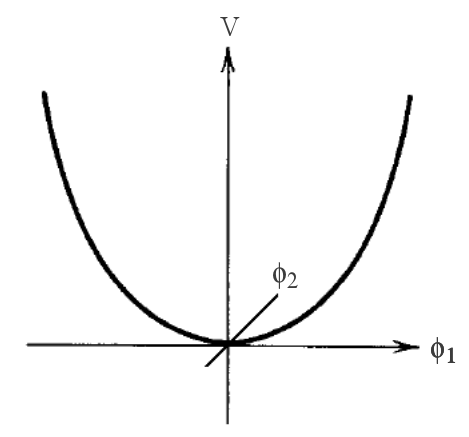
\includegraphics[scale=0.4]{ChapterTheory/figs/mu_pos.png}} \quad \quad
\subfloat[$\mu^2 < 0$]{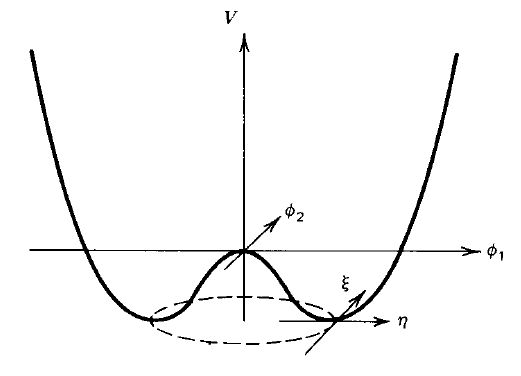
\includegraphics[scale=0.34]{ChapterTheory/figs/mu_neg.png}}
\source{Adapted from \cite{bib:halzen-martin-1984}, p. 322 and 325.}
\label{fig:muPotencial}
\end{figure}

Considering now one of those vacuum states (in terms of $\phi_1$ and $\phi_2$) and making the expansion around the chosen state, one has

\begin{eqnarray}
\langle \phi \rangle &=& \left(\begin{aligned} v \\ 0 \end{aligned} \right) \\ \phi' &\equiv& \phi - \langle \phi_0 \rangle \quad \rightarrow \quad \langle \phi \rangle = \left(\begin{aligned} v +& \eta \\ \xi& \end{aligned} \right).
\end{eqnarray}

Inserting this new displaced field in the lagrangian, it becomes

\begin{equation}
\mathcal{L} = \dfrac{1}{2}[(\partial_{\mu}\eta)^2 + 2\mu^2\eta^2] + \dfrac{1}{2}(\partial_{\mu}\xi)^2 + \mathcal{O}_{sup} + const.
\end{equation}

where, $\mathcal{O}_{sup}$, representing terms of interaction and self interaction of the fields, and the constant are not important in this discussion.

The lagrangian obtained contains two particles: one ($\eta$) with mass $m_{\eta} = \sqrt{-2\mu^2} = \sqrt{2\lambda v^2}$ and one massless particle ($\xi$). The massless particle is a consequence of the lagrangian SO(2) invariance and its origins is stated by the Goldstone Theorem. According to this theorem, a massless scalar arises every time a continuous symmetry is broken, or more specifically, for each generator of the original symmetry group broken there will arise a massless and spinless particle \cite{bib:halzen-martin-1984,bib:griffiths-2008,bib:quigg-1983}. The Higgs mechanism is an extension of the process showed here: an application of the spontaneous symmetry breaking in locally gauge invariant theories.


\subsection{The Brout-Englert-Higgs Mechanism}
In 1963, Phill Andreson proposed that symmetries broken spontaneously would provide a base to explain the massive gauge bosons in non-relativistic systems and later, these ideas were studied in the context of quantum field theories. It was shown that a complex scalar field whose potential is particularly chosen can spontaneously break the gauge symmetry. Peter Higgs suggested that this indicated the existence of a new massive scalar particle. Glashow, Weinberg and Salam showed that the Higgs mechanism could be used to break the gauge symmetry of the electroweak theory and produce the known electroweak interactions. They were even able to predict accurately the mass of the $Z$ boson which has been observed directly in 1983 \cite{bib:PhysLettB-126-1983, bib:EurophysNews-14-10-1983}.

The Higgs boson is the quantum of a scalar field which breaks the electroweak symmetry (EWSSB - \textit{Electroweak Spontaneous Symmetry Breaking}) generating the mass of the $W^{\pm}$ and $Z$ vectorial bosons, providing yet a reasonable base to explain the origin of the leptons and quarks mass \footnote{In the case of neutrinos, in modern theories (since the SM does not include mass for them), it is believed that the Higgs mechanism is not entirely responsible for the neutrinos mass \cite{bib:PhysRevD-86-1-2012}.} \cite{bib:JPhys-447-1-2013}. The understanding of the electroweak symmetry breaking mechanism is one of the most fundamental problems in the Particle Physics and the Higgs discovery is one of the bases for it. 

Exemplifying the Higgs mechanism in the SM be the following lagrangian

\begin{equation}
\mathcal{L} = (\partial_{\mu}\phi)^{*}(\partial^{\mu}\phi) - \mu^2 \phi^{*}\phi - \lambda(\phi^{*}\phi)^2 - \dfrac{1}{4}F_{\mu\nu}F^{\mu\nu}
\label{eq:Lagrangiana_U1}
\end{equation} 

where, $\phi$ is the complex field

\begin{equation}
\phi = \dfrac{\phi_1 \pm i\phi_2}{\sqrt{2}}.
\end{equation}

In order that this lagrangian be invariant under local gauge transformation, that is, $\phi~\rightarrow~e^{iq\alpha(x)}~\phi$, the ordinary partial derivative, $\partial_{\mu}$, needs to be replaced by the so called \textit{covariant} derivative $D_{\mu} = \partial_{\mu} + iqA_{\mu}$ (this is the process in which the interactions are introduced). The gauge field $A_{\mu}$ must also transform as $A_{\mu} \rightarrow A_{\mu} - \partial_{\mu}\theta$ to complete the invariant lagrangian. Considering $\mu^2 < 0$ (condition for the symmetry breaking) the potential has a continuum of degenerated vacuum states at $\langle \vert \phi_0 \vert^2 \rangle = -\mu^2/2\vert \lambda \vert = v^2/2$. Again, by the formalism of the theory, the field $\phi$ must be expanded in terms of a particular vacuum state. Choosing, for instance, $\langle \phi_0 \rangle = v/\sqrt{2}$, the field $\phi$ is conveniently parameterized as

\begin{equation}
\phi = \dfrac{e^{i\xi /v}(v + \eta)}{\sqrt{2}} \simeq \dfrac{(v + \eta + i\xi)}{\sqrt{2}}
\label{eq:phi_SSB}
\end{equation}

which inserted in Eq.~\ref{eq:Lagrangiana_U1} and considering the covariant derivative and the field $A_{\mu}$ transformation, gives

\begin{equation}
\mathcal{L} = \dfrac{1}{2}[(\partial_{\mu}\eta)^2 + 2\mu^2\eta^2] + \dfrac{1}{2}(\partial_{\mu}\xi)^2 - \dfrac{1}{4}F_{\mu\nu}F^{\mu\nu} + qvA_{\mu}\partial^{\mu}\xi + \dfrac{q^2v^2}{2}A_{\mu}A^{\mu} + \mathcal{O}_{sup} + const.
\label{eq:Lagrangiana_SSB}
\end{equation} 

As expected from the Goldstone theorem in the lagrangian of Eq.~\ref{eq:Lagrangiana_SSB} there is a massless field, $\xi$. The term $qvA_{\mu}\partial^{\mu}\xi$ does not have a clear interpretation. Terms like that, bilinear in two different fields, indicate that the fundamental particles of the theory were not correctly identified. Also, note that the lagrangian of Eq.~\ref{eq:Lagrangiana_U1} has four degrees of freedom: two coming from the scalar field $\phi$ and two from the vectorial field $A_{\mu}$. The lagrangian of Eq.~\ref{eq:Lagrangiana_SSB}, however, presents five degrees of freedom: two from the scalar field and three from the vectorial field due to its mass acquisition. Such non-conservation of the degrees of freedom means that exist non-physical fields in the lagrangian. This can be handled by applying the gauge symmetry. Note that the terms involving the fields $\xi$ and $A_{\mu}$ can be written as the combination

\begin{equation}
\dfrac{q^2v^2}{2} \left( A_{\mu} + \dfrac{1}{qv}\partial_{\mu}\xi \right) \left( A^{\mu} + \dfrac{1}{qv}\partial^{\mu}\xi \right)
\end{equation}

which clearly suggests the gauge transformation

\begin{equation}
A_{\mu} \rightarrow A_{\mu}' = A_{\mu} + \dfrac{1}{qv}\partial_{\mu}\xi
\end{equation}

such that,

\begin{eqnarray}
&&\partial_{\mu}A_{\nu}' - \partial_{\nu}A_{\mu}'= \partial_{\mu}A_{\nu} - \partial_{\nu}A_{\mu}
\\ 
&&A_{\mu}'A^{'\mu} = A_{\mu}A^{\mu} + \dfrac{2}{ev}A^{\mu}\partial_{\mu}\xi + \dfrac{1}{e^2v^2}(\partial_{\mu}\xi)^2.
\end{eqnarray}

Note that, this also corresponds to a phase rotation over the field $\phi$ parameterized from Eq.~\ref{eq:phi_SSB} (called unitary gauge)

\begin{equation}
\phi \rightarrow \phi' = e^{-i\xi(x)/v}\phi(x) = (v + \eta)/ \sqrt{2}
\label{eq:gauge_unitario}
\end{equation}

and, as the lagrangian is invariant under local gauge transformations, it is possible to rewrite it as following 

\begin{equation}
\mathcal{L} = \dfrac{1}{2}[(\partial_{\mu}\eta)^2 + 2\mu^2\eta^2] - \dfrac{q^2v^2}{2}A_{\mu}'A^{'\mu} - \dfrac{1}{4}F_{\mu\nu}F^{\mu\nu} + \mathcal{O}_{sup} + const.
\label{eq:hg_lagrangian}
\end{equation}

The Eq.~\ref{eq:hg_lagrangian} summarizes the Higgs mechanism. The terms between the brackets form a Klein-Gordon field associated to a massive particle while the other two terms represent a vectorial field associated to a massive gauge boson. It is interesting to observe as the gauge boson appears in the lagrangian. The original field $A_{\mu}$ has just two degrees of freedom (as the photon has just two polarizations). However, the Goldstone boson, also without mass and which appears from the spontaneous continuous symmetry breaking, combines with the gauge field in order to give it a longitudinal degree of freedom: the mass. Note that, the Goldstone does not disappear from the theory, it just is not explicitly apparent anymore due to the new gauge (Eq.~\ref{eq:gauge_unitario}) used in the lagrangian. The remaining component of the parameterized field $\phi$, that is, the scalar field $\eta$, is the so called Higgs boson. This phenomenon of a gauge boson acquiring mass by "absorbing" a Goldstone boson is the Higgs mechanism: a combination of local gauge invariance and the spontaneous symmetry breaking \cite{bib:griffiths-2008,bib:halzen-martin-1984,bib:quigg-1983,bib:das-2008}.


\subsection{The Higgs Mechanism and Electroweak Symmetry Breaking}
The elementary particles interacting weakly are described by multiplets belonging to the weak isospin group SU(2). Furthermore, only the components left-handed of the fermionic fields participates in the electroweak interactions, so that, the isospin group is often identified as $SU_{L}(2)$. This means that only such components are modified on symmetry transformations. Experimentally it is observed that the weak interactions violate the weak isospin and hipercharge symmetries. In other words, the particles do not conserve the quantum numbers associated to these symmetries in process guided by weak interactions. The hipercharge is a quantum number associated to the symmetry group U(1), which combined to the third component of the isospin, as $Q = I_3 + Y/2$, comports the values of electric charge of each particle weakly interacting \cite{bib:das-2008,bib:seiden-2008}. 

As already mentioned, the theories involved in the SM are locally gauge invariants, which contains massless fields. However, the weak processes are marked by interactions of short range, what is translated in the existence of an associated massive boson as the mediator of the interaction. In such way, the Higgs mechanism is associated to the breaking of the isospin and hipercharge symmetries, and the theory is constructed over the symmetry group $SU_L(2) \times U(1)_Y$. Additionally, the breaking of the symmetry must occur in such way that the electroweak symmetry survives, keeping a massless gauge field (the photon). Schematically the electroweak symmetry breaking is, then, represented as $SU_L(2) \times U_Y(1) \rightarrow U_{em}(1)$. The gauge fields, that are expected to result in mediators, are determined by the structure of the local symmetry of the theory. Thus, three vectorial fields are introduced for the $SU_L(2)$ symmetry and a vectorial field for the $U_Y(1)$ symmetry (for instance, $W_{\mu}^a \quad (a=1,2,3)$ and $Y_{\mu}$, respectively) \cite{bib:ellis-2003}. The electroweak lagrangian can, then, be written as

\begin{equation}
\mathcal{L} = \left( \partial^{\mu}\phi^{\dagger} + ig W^{\mu}.T\phi^{\dagger} + \dfrac{1}{2}ig' Y^{\mu}\phi^{\dagger} \right) \left( \partial_{\mu}\phi - ig W_{\mu}.T\phi - \dfrac{1}{2}ig' Y_{\mu}\phi \right) + \mu^{2}\phi^{\dagger}\phi - \lambda(\phi^{\dagger}\phi)^{2}
\end{equation}

where, $g$ and $g'$ correspond to the coupling constants for the gauge interactions associated to the symmetry groups $SU_L(2)$ and $U_Y(1)$, respectively. These constants have the following relation with the Weinberg angle (electroweak mixture angle)

\begin{equation}
\textrm{sen}^{2}~\theta_W = \dfrac{g'^{2}}{g^{2}+g'^{2}} \approx 0.23
\end{equation}

The Higgs field is also described by a multiplet of $SU(2)$, whose minimum configuration capable to generate the expected symmetry breaking is given by the doublet of complex fields

\begin{equation}
\phi = \left(\begin{aligned} \phi^{+} \\ \phi^{0} \end{aligned} \right) = \sqrt{\dfrac{1}{2}} \left(\begin{aligned} \phi_1 + i\phi_2 \\ \phi_3 + i\phi_4 \end{aligned} \right)
\label{eq:Higgs_dubleto}
\end{equation}

where, the field $\phi^{+}$ has charge $Q=1$ and the field $\phi^{0}$ has charge $Q=0$. As exemplified in the previous sections, the mass of the gauge bosons is identified after the symmetry breaking done by the choice of a particular vacuum state to expand the field $\phi$. In this procedure, the gauge freedom is used again in order to write the lagrangian containing only physical fields, which is often achieved by using the gauge

\begin{equation}
\phi = \sqrt{\dfrac{1}{2}} \left( \begin{aligned} 0 \quad \quad \\ v+h(x) \end{aligned} \right)
\end{equation}

In the end, the massive gauge bosons arise through the combination of the fields $W_{\mu}^{1,2}$ (for the bosons $W^{\pm}$) and of the fields $Y_{\mu}$ and $W_{\mu}^3$ (for the bosons $Z$ and $\gamma$ - the photon) through the expressions

\begin{eqnarray}
\left. \begin{aligned} &W_{\mu}^{\pm} = \dfrac{(W^1 \mp iW^2)}{\sqrt{2}},& \quad &M_W = \dfrac{vg}{2}&\\[0.1cm]
&Z_{\mu} = \dfrac{gW_{\mu}^3 - g' Y_{\mu}}{\sqrt{g^2+g^{'2}}},& \quad &M_Z = \dfrac{v\sqrt{g^2+g^{'2}}}{2}& \end{aligned} \right\} (\textrm{electroweak vector bosons})
\end{eqnarray}

\begin{eqnarray}
\left. A_{\mu} = \dfrac{g'W_{\mu}^3 + gY_{\mu}}{\sqrt{g^2+g^{'2}}}, \quad \quad \quad M_{\gamma} = 0 \quad \right. (\textrm{photon})
\end{eqnarray}

where, the parameter $v \approx 246$ GeV is the expected vacuum value of the Higgs field. It is interesting to note that, in order to generate the leptons and quarks mass (Yukawa sector) the same Higgs doublet (Eq.~\ref{eq:Higgs_dubleto}) can be used. For the leptons the application is immediate, while for the quarks, which have the fields in the up part of the doublets also massive\footnote{The lepton doublets are composed by a lepton and its respective neutrino, which in the SM is considered massless.}, it is needed a new doublet obtained from the Eq.~\ref{eq:Higgs_dubleto} \cite{bib:halzen-martin-1984}.


\section{The Higgs Boson at the LHC}
The standard model (SM) of electroweak interactions relies on the existence of the Higgs boson, the scalar particle associated with the field responsible for spontaneously breaking electroweak symmetry \cite{bib:PhysRev22-579-1961,bib:PhysRevLett19-1264-1967}. The ATLAS and CMS collaborations reported in 2012 for the first time the discovery of a new boson consistent with the SM Higgs [3-8] by observing proton-proton (pp) collisions from the LHC at $\sqrt{s}=$ 7 and 8 TeV. Several studies carried out by CMS and ATLAS, and the combination of these results, have shown so far that the properties of the observed scalar boson is consistent with the SM expectations \cite{bib:CMS-PAS-HIG-14-038,bib:ATLAS-CONF-2015-004,bib:JPhys-455-1-2013,bib:CMS-HIG-13-002,bib:PhysRevLett110-081803-2013,bib:PhysRevD89-092007-2014}. 

At the LHC, the Higgs boson can be produced in four main modes (the most significant in terms of their cross section). These modes are \cite{bib:ellis-2003}:

\begin{flushleft}
	\quad a) Gluon fusion: $gg \rightarrow H$;
	
	\quad b) Vector boson fusion (VBF): $qq \rightarrow Hqq$;
	
	\quad c) Vectorial boson association (Higgstrahlung): $q \overline{q} \rightarrow WH/ZH$;
	
	\quad d) Top quark association: $gg/q \overline{q} \rightarrow t \overline{t} H$.
\end{flushleft}

\begin{figure}[htbp]{15cm}
	\caption{The main Higgs (represented by the dotted line) production modes at the LHC.}
	\subfloat[Gluon fusion]{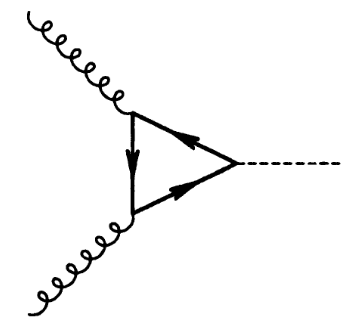
\includegraphics[scale=0.3]{ChapterTheory/figs/ggH.png}}
	\subfloat[Vector boson fusion]{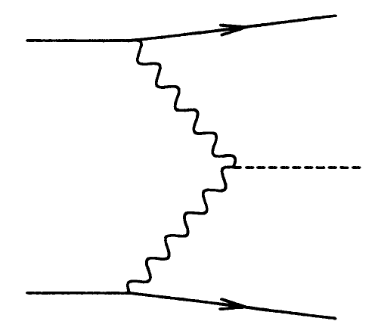
\includegraphics[scale=0.3]{ChapterTheory/figs/VBF.png}}
	\subfloat[Higgs-strahlung]{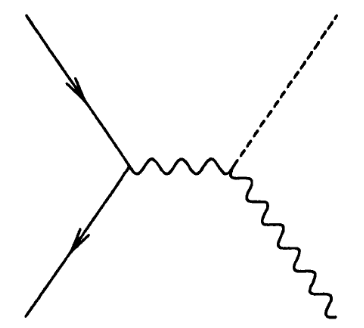
\includegraphics[scale=0.3]{ChapterTheory/figs/AssWZ.png}}
	\subfloat[Associated production with top quark]{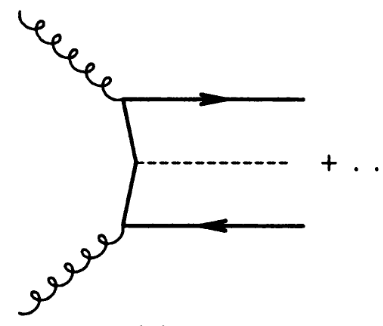
\includegraphics[scale=0.3]{ChapterTheory/figs/Ass_tt.png}}
	\source{Reference \cite{bib:ellis-2003}, p. 398.}
	\label{fig:Higgs_pro_mechanisms}
\end{figure}

The Feynman diagrams at LO (\textit{leading-order}) for each of this processes are shown in Fig.~\ref{fig:Higgs_pro_mechanisms}. The gluon fusion is the production mode in which the Higgs is produced through a loop of top quarks induced by the interaction of gluons in the initial state. This is the production mode with the highest probability to happen, presenting a cross section of about 43.9 pb for $m_{H} = $ 125GeV at $\sqrt{s} = $13TeV \cite{bib:LHC-Higgs-XSWG-2018}. 

The second most important production mode is the vector boson fusion. In this production mode the Higgs is created by the fusion of weak vectorial bosons ($Z$, $W^{\pm}$) which arises during the scattering of quarks in the colliding protons. The main characteristic of this mode is the presence of two energetic jets in the final state and separated by a pseudorapidity gap. Its cross section at 13TeV for $m_{H} = $125GeV is about 3.7 pb \cite{bib:LHC-Higgs-XSWG-2018,bib:IFAE-14-2008,bib:PhysRevD98-030001-2018}.

The cross section of the Higgs production associated to vectorial bosons is even smaller, but they are useful for observing the Higgs decaying into $b\bar{b}$ or $\gamma\gamma$ since the decay can be tagged by the presence of the bosons $W/Z$. The production of Higgs up to $M_{H} \sim 400~GeV$ associated to quark top is the smallest one between the main production modes. This process is similar to the Higgstrahlung, but the Higgs in this case is emitted from top quarks through $gg$ or $q\bar{q}$ interactions \cite{bib:ellis-2003}.

The Higgs can decay in several final states and each of them presents advantages and disadvantages. The decaying channel $ZZ \rightarrow 4l$, handled in this analysis, is one of the best ones. This channels is actually called "the golden channel" because all the decay products can be fully reconstructed in the CMS detector and it also has relatively small backgrounds at the signal region. However, the branching ratio (BR) into $ZZ \rightarrow 4l$ is small, about 3.3x10$^{-6}$ for $m_{H} = $125GeV at 13TeV \cite{bib:LHC-Higgs-XSWG-2018}. The Fig.~\ref{fig:Higgs_XSBR} shows in (a) the Higgs cross sections for different center-of-mass energies and in (b) its branching ratios at 13TeV (the energy in which this analysis have been done).

\begin{figure}[htbp]{15cm}
	\caption{Higgs production cross section and branching ratios.}
	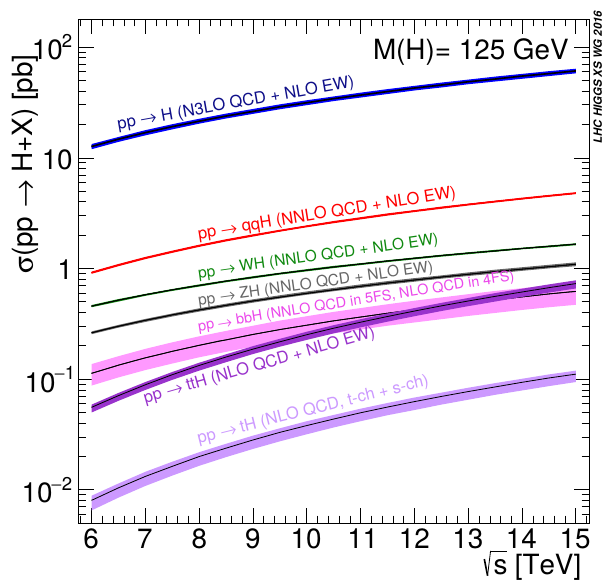
\includegraphics[scale=0.4]{ChapterTheory/figs/Higgs_XS_vs_S.png}
	\quad
	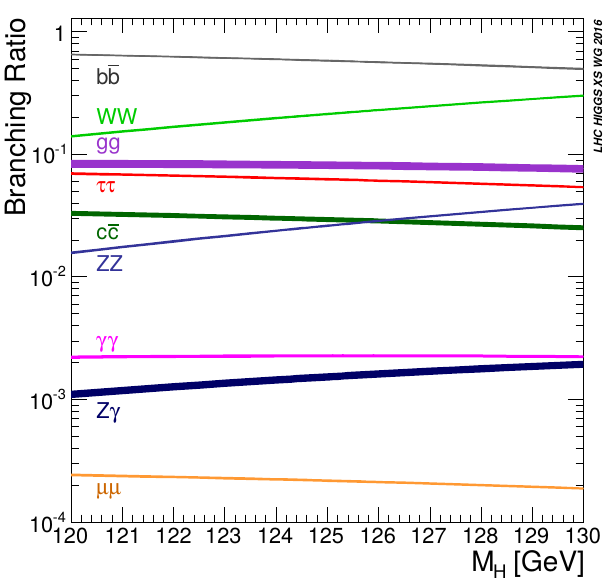
\includegraphics[scale=0.4]{ChapterTheory/figs/Higgs_BRs.png}
	\source{Reference \cite{bib:PhysRevD98-030001-2018}, p. 184.}
	\label{fig:Higgs_XSBR}
\end{figure}

\section{The Higgs VBF Production Mode \label{sec:vbf_theory}}
Many measurements of the properties of the Higgs boson are still statistics limited, and there is still significant room for beyond standard model effects in the Higgs sector. A particularly sensitive channel for observing non-standard model effects is the cross section for Higgs boson production through the Vector Boson Fusion (VBF) mode. There are some special features about this production mode. It has the largest cross section between the processes that involves tree-level production of the Higgs boson. It is also the second largest among all the processes. Its signature of two energetic forwarded jets makes possible to tag events and identify Higgs decays that normally have large backgrounds. Another feature is that the Higgs $p_{T}$ is nonzero, even at lowest order, facilitating searches of invisible decay modes. The VBF mode also has a particular sensitivity to the charge-parity properties of the Higgs boson and non-standard Higgs interactions via  the angular correlations between the jets \cite{bib:Dittmaier_et_al_2011,bib:Dittmaier_et_al_2012,bib:Dittmaier_et_al_2013,bib:CMS-PAS-HIG-14-038,bib:ATLAS-CONF-2015-004,bib:PhysRev88-051801-2002}.

\subsection{The Higgs VBF LO Cross Section and its Kinematics}
\begin{figure}[htbp]{15cm}
	\caption{Feynman diagram for the Higgs production via vector boson fusion. The initial state quarks (or anti-quarks) are $p_{1}$ and $p_{2}$, while the momentum at final state are $p_{1}'$ and $p_{2}'$, respectively.}
	\begin{overpic}
		[scale=0.35]{ChapterTheory/figs/VBF}
		\put(-5,80){$p_{1}$}
		\put(-5,10){$p_{2}$}
		\put(100,85){$p_{1}'$}
		\put(100,5){$p_{2}'$}
		\put(100,45){$H$}
		\put(60,55){$V$}
		\put(60,20){$V$}
	\end{overpic}
	\source{Adapted from \cite{bib:PhysLettB136-3-1984}, p. 196.}
	\label{fig:vbf_labeled_diagram}
\end{figure}

Assuming the Higgs production via the VBF mode as shown in Fig.~\ref{fig:vbf_labeled_diagram}, the matrix element for this process, in terms of the momentum of the involved particles, can be expressed as \cite{bib:PhysLettB136-3-1984}

\begin{equation}
\mathcal{M} = g_{VVH}~\frac{\bar{u}(p_{1}')\gamma^{\lambda}(g_{V}+g_{A}\gamma_{5})\bar{u}(p_{1})~\bar{u}(p_{2}')\gamma_{\lambda}(g_{V}'+g_{A}'\gamma_{5})\bar{u}(p_{2})}{(q_{1}^{2}-M_{V}^{2})~(q_{2}^{2}-M_{V}^{2})},
\end{equation}

where for,

\begin{multicols}{2}
$V = W$:
\begin{eqnarray}
g_{VVH} \rightarrow g_{WWH} = gM_{W}\\
g_{V} = -g_{A} = \frac{e}{2\sqrt{2}~sin~\theta_{W}}
\end{eqnarray}
$V = Z$:
\begin{eqnarray}
g_{VVH} \rightarrow g_{ZZH} = \frac{gM_{W}}{cos^{2}\theta_{W}}\\
g_{V} = \frac{g(T_{3L}/2 - Q~sin^{2}\theta_{W})}{cos~\theta_{W}}\\
g_{A} = - \frac{gT_{3L}}{2~cos~\theta_{W}}.
\end{eqnarray}
\end{multicols}

The term $g = e/sin~\theta_{W}$ is the weak SU(2) gauge coupling and the terms $T_{3L}$ and $Q$ stand for the third component of the weak isospin and the quark charge\footnote{For quarks and leptons $T_{3L} \pm 1/2$.}, respectively. Now, using $g_{L} = (g_{V}-g_{A})/2$ and $g_{L} = (g_{V}+g_{A})/2$ the average squared matrix element becomes \cite{bib:PhysLettB136-3-1984,bib:PhysRep457-1-2005,bib:NuclPhysB287-1987}

\begin{equation}
|\mathcal{M}|^{2} = 64~g_{VVH}^{2}~\frac{C_{1}(p_{1}.p_{2})(p_{1}'.p_{2}') + C_{2}(p_{1}.p_{2}')(p_{1}'.p_{2})}{(q_{1}^{2}-M_{V}^{2})^{2}~(q_{2}^{2}-M_{V}^{2})^{2}}
\end{equation}

where $C_{1} = g_{L}^{2}g_{L}^{'2} + g_{R}^{2}g_{R}^{'2}$ and $C_{1} = g_{L}^{2}g_{R}^{'2} + g_{R}^{2}g_{L}^{'2}$. The differential cross section at LO is, then, given by \cite{bib:PhysRep457-1-2005}

\begin{equation}
d\hat{\sigma}_{LO} = \frac{1}{72}\frac{1}{(2\pi)^{5}}\frac{1}{\hat{s}}~|\mathcal{M}|^{2}~\frac{d^{3}p_{H}}{2dE_{H}}~\frac{d^{3}p_{1}'}{2dE_{1}'}~\frac{d^{3}p_{2}'}{2dE_{2}'}~\delta^{4}(p_{1}+p_{2}-p_{1}'-p_{2}'-p_{H})
\end{equation}

in which the integration over the variables $p_{1}'$ and $p_{2}'$ is conveniently performed in the rest frame of the final-state quarks ($\vec{p}_{1}' + \vec{p}_{2}' = 0$), leading to \cite{bib:PhysRep457-1-2005}

\begin{equation}
\frac{d\hat{\sigma}_{LO}}{dE_{H}~dcos~\theta} = \frac{G_{F}^{3}M_{V}^{8}}{9\sqrt{2}\pi^{3}\hat{s}}~\frac{p_{H}}{32s_{1}s_{2}}~(C_{1}\mathcal{H}_{1} + C_{2}\mathcal{H}_{2})
\label{eq:vbf_dxs_lo}
\end{equation}

where $\hat{s} = (p_{1}+p_{2})^{2}$ is the energy at the CM (\textit{center of mass}), $G_{F}$ is the Fermi constant, $s_{1,2} = \sqrt{\hat{s}}[(\sqrt{\hat{s}}-E_{H}) \pm p_{H}cos~\theta]$, with $p_{H}$ being the Higgs momentum and $\theta$ the final-state parton scattering angle\footnote{Do not confuse that with the $\theta_{W}$, which is the weak-mixing angle (Weinberg angle).}. The $\mathcal{H}_{1,2}$ are terms depending on $s_{1,2}$, $\hat{s}$, $p_{H}$, $\theta$ and $M_{V}$. For the interested reader, please see \cite{bib:PhysRep457-1-2005}.

The total partonic cross section of the Higgs produced via VBF is obtained by integrating the Eq.~\ref{eq:vbf_dxs_lo}, which can properly be done in terms of the Higgs transverse momentum and rapidity as

\begin{equation}
\hat{\sigma}_{LO}(qq \rightarrow Hqq) = \int_{y-}^{y+}dy~\int_{0}^{p_{T}^{max}}dp_{T}~(2\pi p_{T})~\frac{d^{2}\hat{\sigma}_{LO}}{dydp_{T}}.
\label{eq:vbf_xs_lo}
\end{equation}

The integration on $y$ and $p_{T}$ on Eq.~\ref{eq:vbf_xs_lo} can not be done analytically and numerical integration is used to get physical results \cite{bib:PhysRep457-1-2005,bib:NuclPhysB287-1987}. As reported on this previous references, the results show that the quarks at the final state present large energies while their transverse momentum is usually $p_{T} \sim M_{V}$ but, varying with $m_{H}$ (see Fig.~3.14 of \cite{bib:PhysRep457-1-2005} and Fig.~6 of \cite{bib:NuclPhysB287-1987}, for instance). The relatively small transverse momentum of the final-state partons can be translated into a small scattering angles, which in terms of pseudorapidity ($\eta$), means that, the rising jets are forward (a well known signature of VBF).


\subsubsection{Corrections of Higher Orders}
Through the past years considerable enhancements have been achieved in the phenomenological interpretation of the Higgs VBF production mode. Computations for the total cross section and differential distributions to Higgs produced via VBF and including NLO QCD and EW corrections were presented by \cite{bib:Phys46-203-1998,bib:PhysRevLett69-3274-1992} and are available in flexible parton-level Monte Carlo (MC) generators. Partial NNLO QCD corrections have also been presented by \cite{bib:PhysRevD77-053010-2008,bib:PhysRevLett105-011801-2010}, which reduces the uncertainties on the inclusive VBF cross section from 5-10$\%$ to 1-2$\%$, making VBF the theoretically most accurate production mode at hadron colliders \cite{bib:ChinPhysC-38-9-2014}. 

The most recent developments done on the VBF theory formalism comes from the application of the so called \textit{structure function approach}, which is based on the description, in very good approximation, of the VBF process as a double deep-inelastic scattering process (DIS), see Fig.~\ref{fig:vbf_DIS_approx}. In such approximation the two virtual vector bosons $V*_{1,2}$ are independently emitted from the hadronic initial states and fuse into the Higgs boson. 

\begin{figure}[htbp]{15cm}
	\caption{Sketch of the Higgs VBF production description through the structure function approach.}
	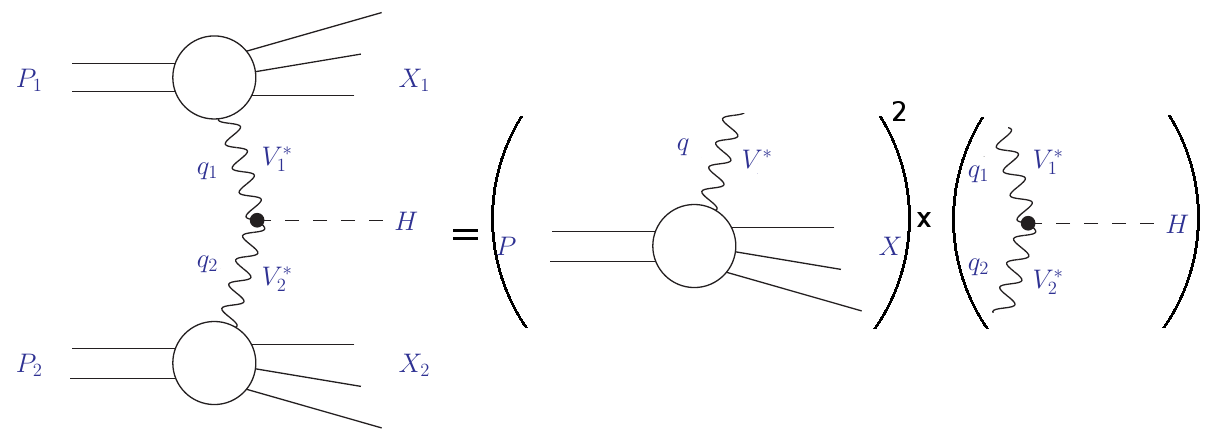
\includegraphics[scale=0.4]{ChapterTheory/figs/vbf_DIS_approximation}
	\source{Adapted from \cite{bib:PhysRevLett105-011801-2010}, p. 3.}
	\label{fig:vbf_DIS_approx}
\end{figure}

This approximation builds on the absence (or smallness) of QCD interference between the two inclusive final states $X_{1}$ and $X_{2}$. The total cross section is given as a product of the matrix element $\mathcal{M}^{\mu\nu}$ for VBF ($V_{1}^{\mu}V_{2}^{\nu} \rightarrow H$) and the DIS hadronic tensor $W_{\mu\nu}$, giving a VBF differential cross section of the form \cite{bib:PhysRevLett105-011801-2010,bib:PhysRevLett69-3274-1992},

\begin{eqnarray}
\nonumber
d\sigma = \frac{1}{2s}2G_{F}^{2}~M_{V_{1}}^{2}M_{V_{2}}^{2}~\frac{1}{(Q_{1}^{2}+~M_{V_{1}}^{2})^{2}}~\frac{1}{(Q_{2}^{2}+~M_{V_{2}}^{2})^{2}}\times\\
\nonumber
W_{\mu\nu}(x_{1},Q_{1}^{2})\mathcal{M}^{\mu\rho}\mathcal{M}^{*\nu\sigma}W_{\rho\sigma}(x_{2},Q_{2}^{2})\times\\ \frac{d^{3}P_{X_{1}}}{(2\pi)^{3}2E_{X_{1}}}~\frac{d^{3}P_{X_{2}}}{(2\pi)^{3}2E_{X_{2}}}~ds_{1}ds_{2}~\frac{d^{3}P_{H}}{(2\pi)^{3}2E_{H}}
(2\pi)^{4}~\delta^{4}(P_{1}+P_{2}-P_{X_{1}}-P_{X_{2}}-P_{H}),
\label{eq:vbf_dis_differential_XS}
\end{eqnarray}

where, $s$ stands for the center-of-mass energy of the collider, $G_{F}$ is the Fermi's constant, $Q_{1}^{2} = -q_{i}^{2}$ and $x_{i} = Q_{i}^{2}/(2P_{i}.q_{i})$ are the usual DIS variables, $M_{V_{i}}$ stands for the vector boson mass. The hadronic tensor $W_{\mu,\nu}$ represents the unknown physics at the $V_{\mu,\nu}^{1,2}$-parton vertexes. This function depends on the four-momentum of both vector boson and the parton. 

The theoretical discussion about the full computation of the total cross section exceeds the scope of this analysis and it will not be presented here. For the reader interested in more details, please have a look on \cite{bib:PhysRep457-1-2005}, \cite{bib:PhysRevLett69-3274-1992} and \cite{bib:PhysRevLett105-011801-2010}.


\section{The Physics Scenario of this Analysis}
The VBF production mode, as presented on previous sections, is a key process for precision measurements of Higgs properties since it is a clean channel with very distinctive kinematics. Such features provide good scenario for measurements of Higgs couplings \cite{bib:PhysRevD62_013009_2000}. The VBF channel is a direct probe of the coupling between vector bosons and the Higgs boson, and hence directly probes the electroweak sector of the standard model.

Additionally, the $H \rightarrow ZZ \rightarrow 4l$ (l = e, $\mu$) decay channel has a large signal-to-background ratio because it is possible to completely reconstruct the final state leptons, which presents excellent momentum resolution. This feature makes this decay channel one of the most important for the studies of the Higgs boson properties. Several different measurements have been performed with the data collected during the LHC RunI using this channel
\cite{bib:PhysRevLett110-081803-2013,bib:PhysRevD89-092007-2014,bib:PhysLettB-736-64-2014,bib:PhysRevD92-012004-2015,bib:PhysRevD92-072010-2015}. This decay channel, thus, presents a good frame to measure Higgs VBF production.

This analysis presents a measurement of the Higgs boson VBF production cross-section obtained in the $H \rightarrow ZZ \rightarrow 4l$ decay channel using data collected at $\sqrt{s}=$ 13TeV. The data accounts for 35.9$fb^{-1}$ of pp collision collected with the CMS detector at the LHC RunII in 2016. This analysis uses similar requirements as the CMS $HZZ4L$ 2016 analysis \cite{bib:CMS-AN-16-442} and \cite{bib:CMS-AN-16-328}, relying essentially on the reconstruction, identification and isolation of leptons and requiring the presence of jets and Missing Energy Transverse (MET). The specific selection and analysis requirements will be discussed in more detail in the following sections.

As it will also be shown, the main processes in this analysis, besides the VBF itself, are the $gg \rightarrow H$ Higgs production mode and the reducible SM background $q\bar{q} \rightarrow ZZ$ (which in the context of the present analysis become a non-reducible background). In a smaller, but still significant, contribution appears the remaining Higgs production modes, Higgs-strahlung (VH) and associated with top quark ($t\bar{t}H$), and the SM background $gg \rightarrow ZZ$. The tree-level Feynman diagrams for each of these processes are shown in Fig.~\ref{fig:processes_feynman}.

\begin{figure}[htbp]{16cm}
	\caption{Main processes in this analysis: Higgs production modes (a) vector boson fusion (VBF), (b) gluon-fusion (ggH), (c) Higgsstrahlung (VH), (d) production associated to top quark, and the main SM backgrounds (e) and (f) ZZ. Additionally there is the $Z+X$ background which is derived via the Fake Rate \textit{data-driven} method and will be presented later.}
	\centering
	\subfloat[$q\bar{q} \rightarrow Hq\bar{q}$]{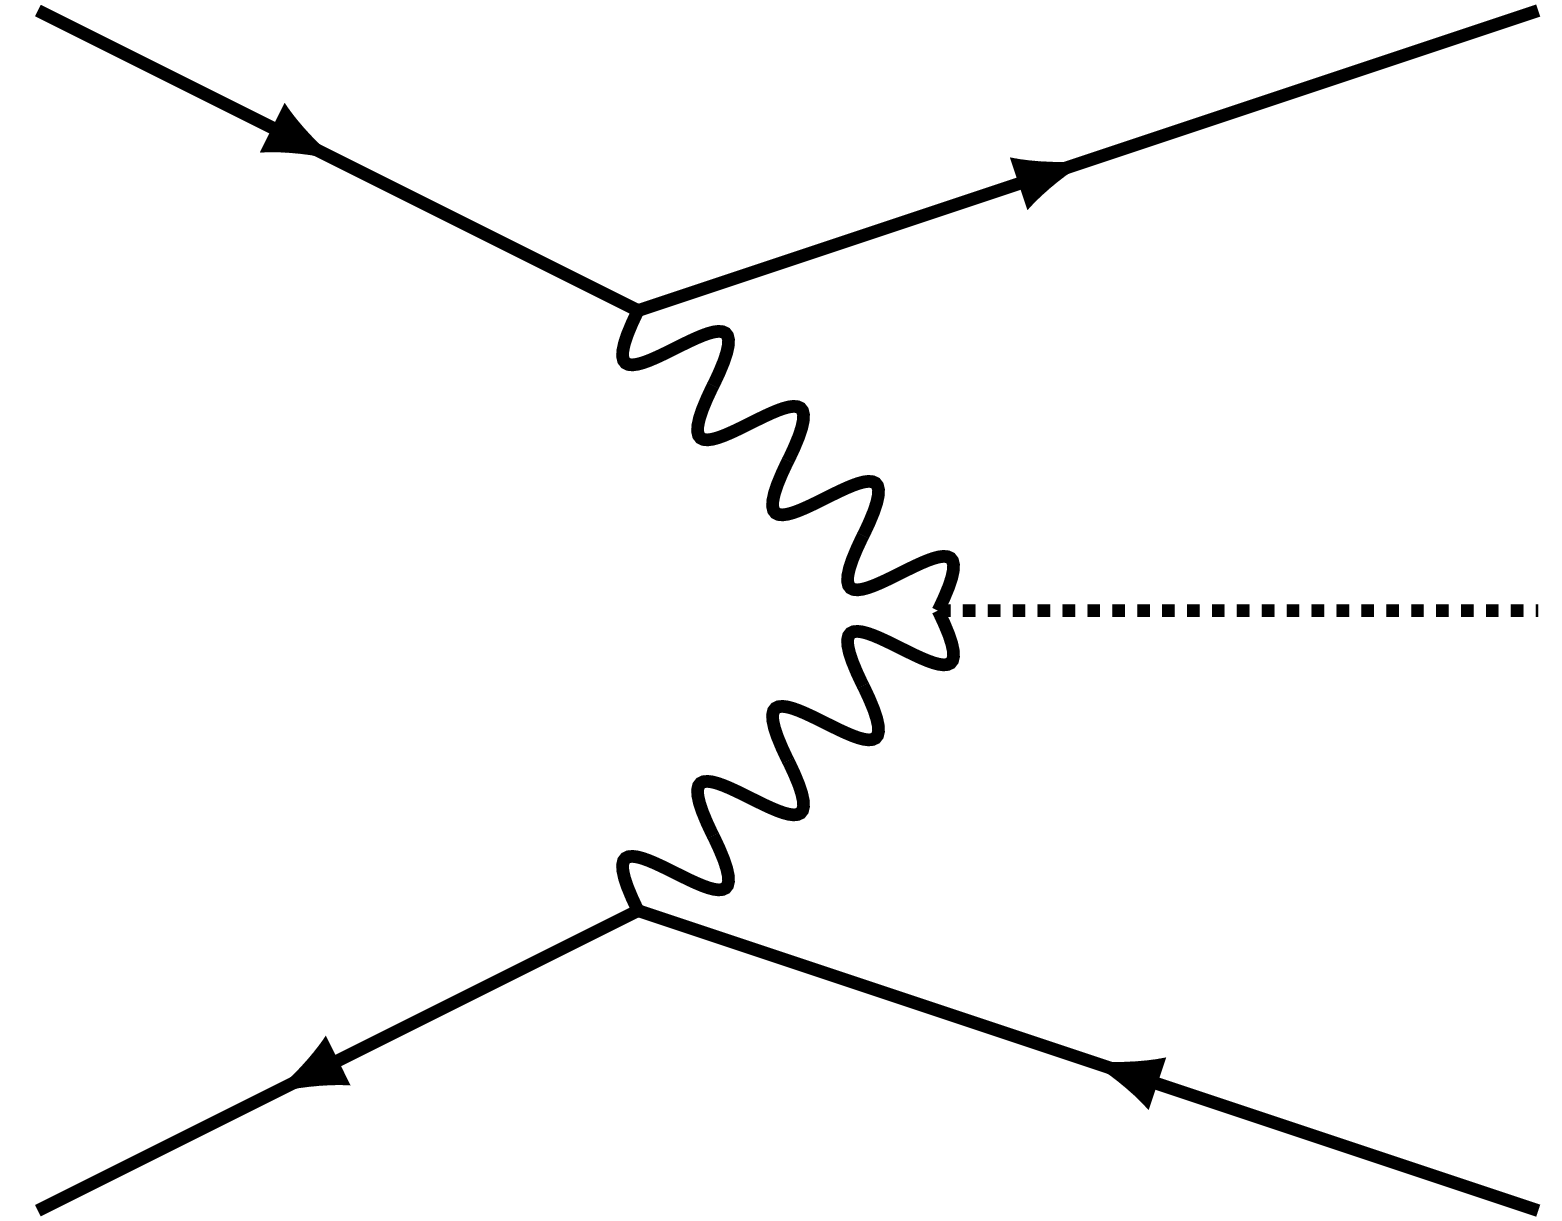
\includegraphics[scale=0.08]{ChapterAnalysis/figs/vbf_diagram}}
	\quad\quad
	\subfloat[$gg \rightarrow H$]{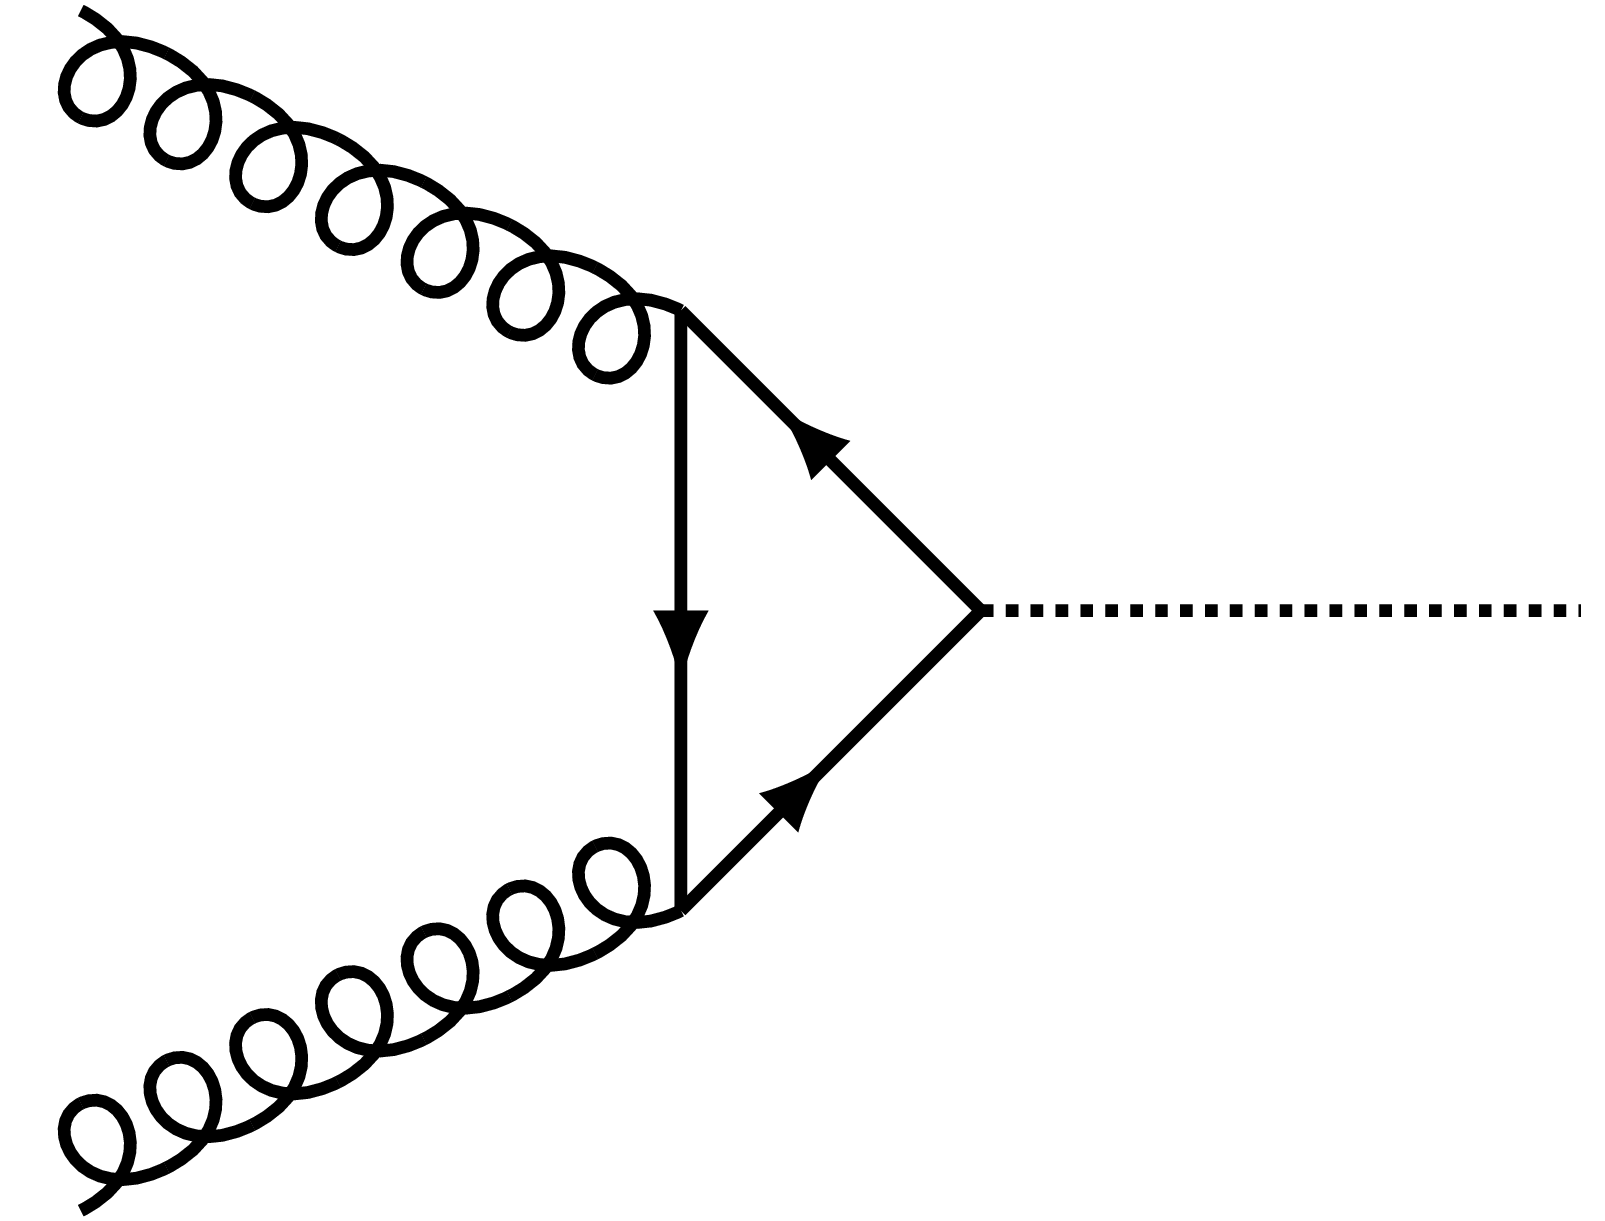
\includegraphics[scale=0.08]{ChapterAnalysis/figs/ggh_diagram}}
	\quad\quad
	\subfloat[$q\bar{q} \rightarrow VH$]{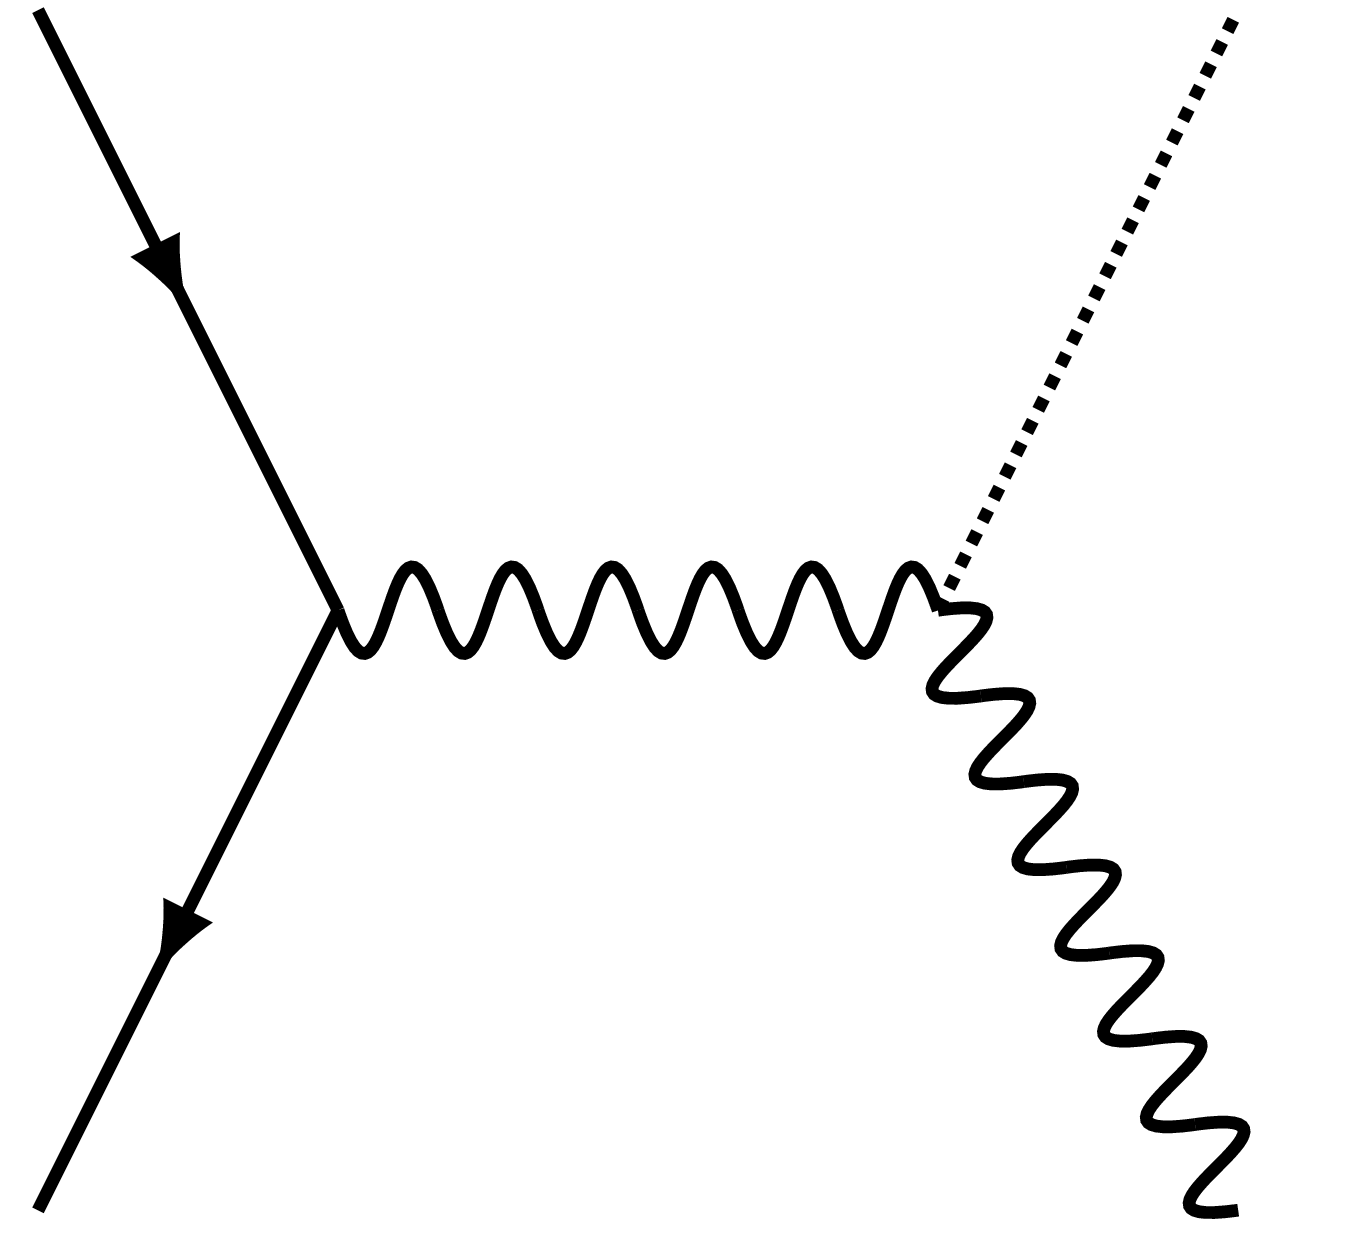
\includegraphics[scale=0.08]{ChapterAnalysis/figs/vh_diagram}}\\
	\subfloat[$gg \rightarrow t\bar{t}H$]{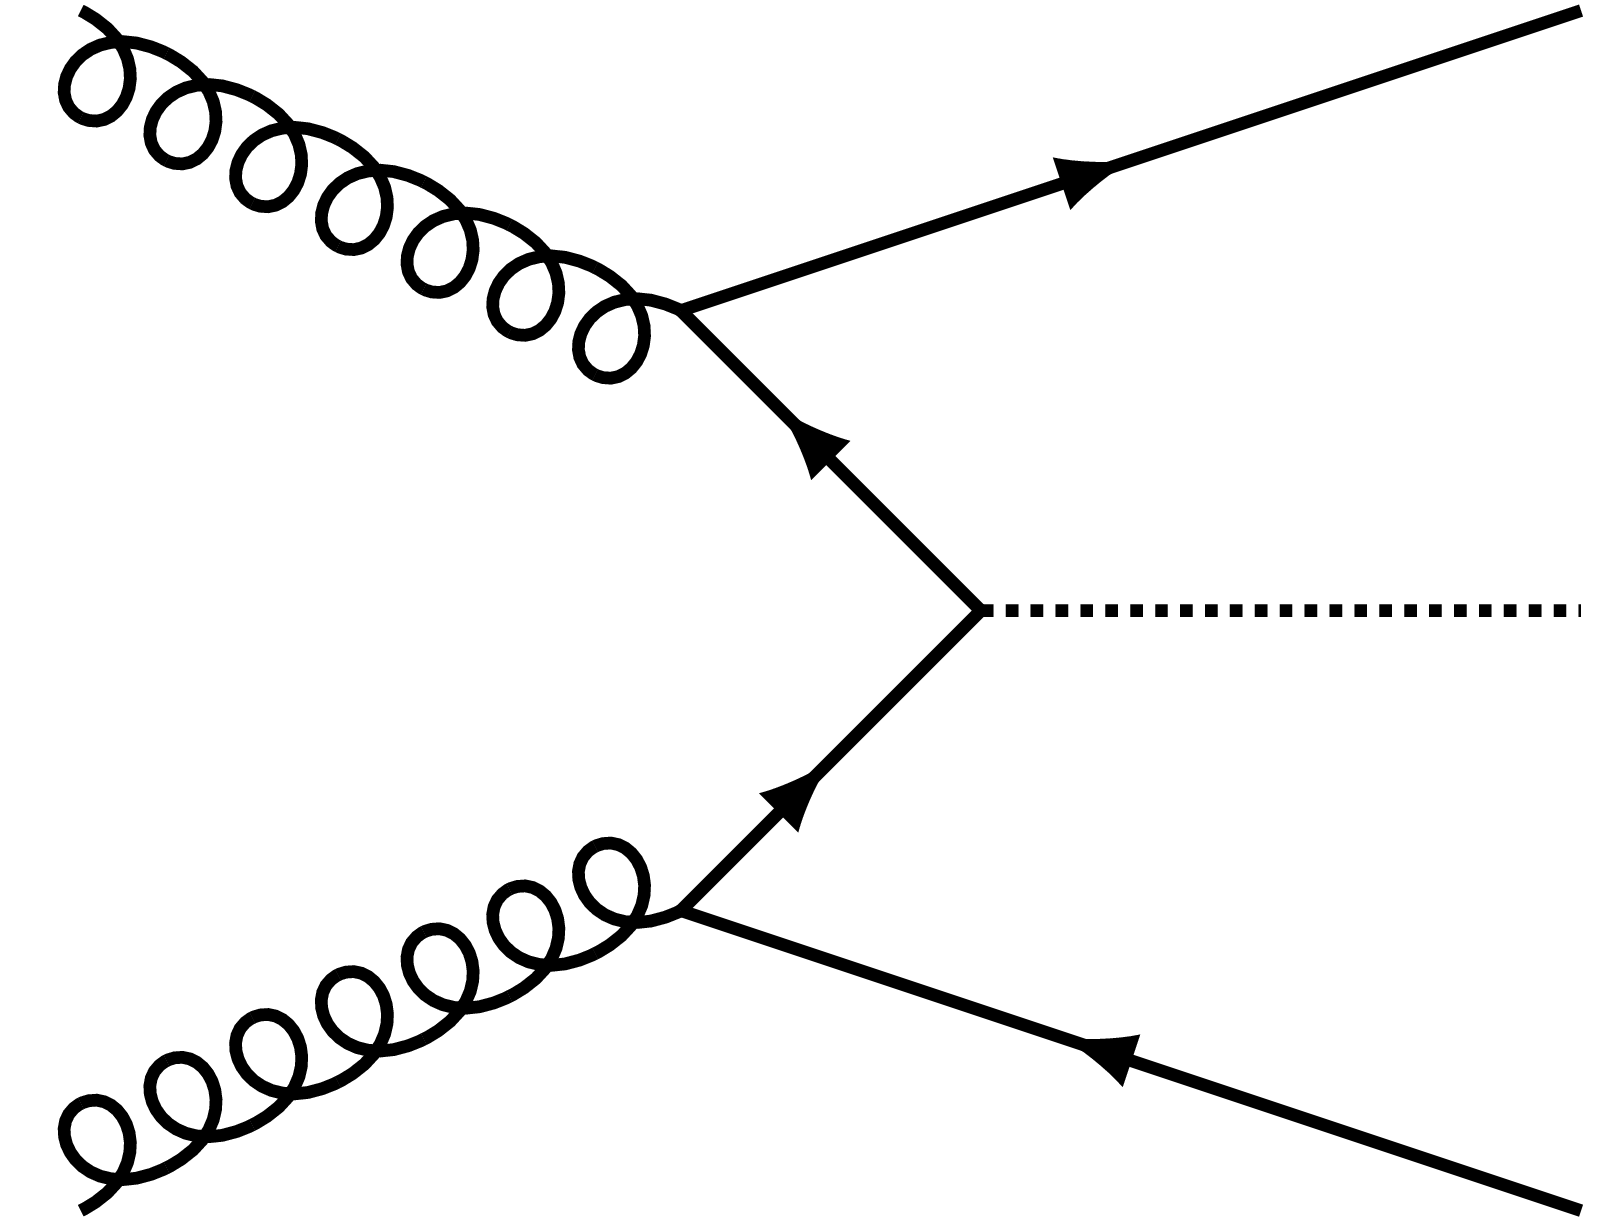
\includegraphics[scale=0.08]{ChapterAnalysis/figs/tth_diagram}}
	\quad\quad
	\subfloat[$q\bar{q} \rightarrow ZZ$]{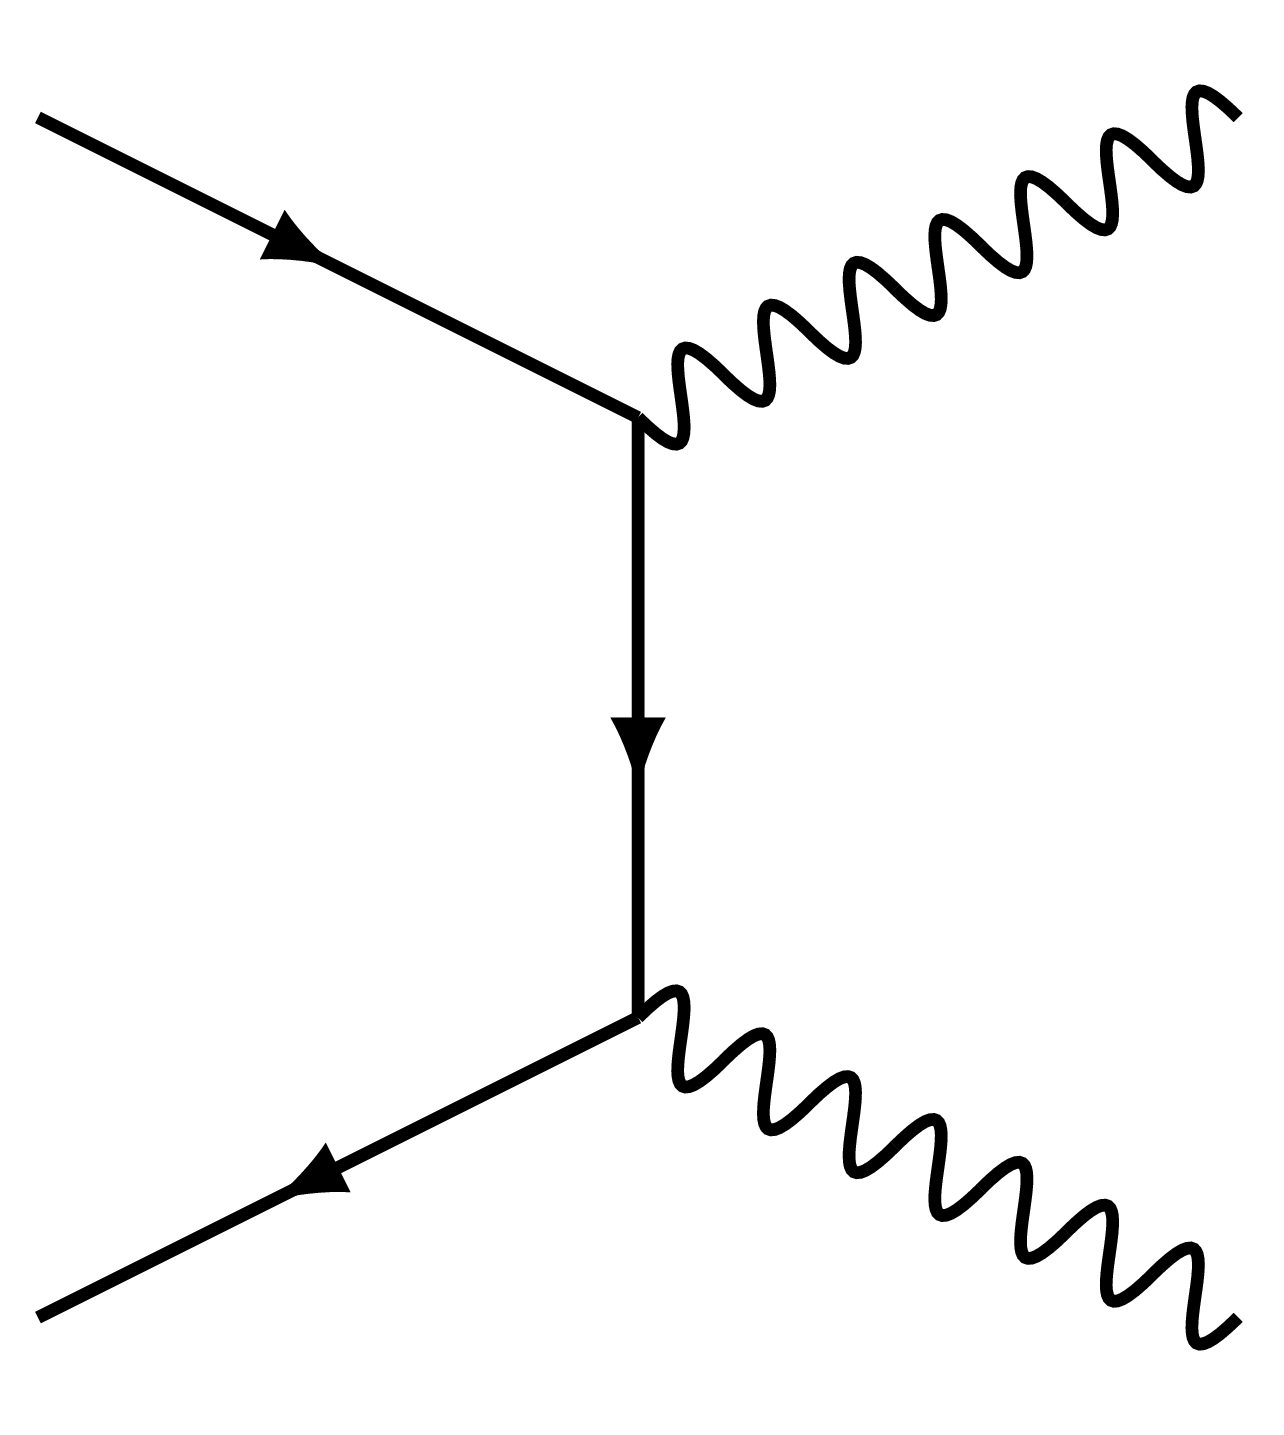
\includegraphics[scale=0.08]{ChapterAnalysis/figs/qqzz_diagram}}
	\quad\quad
	\subfloat[$gg \rightarrow ZZ$]{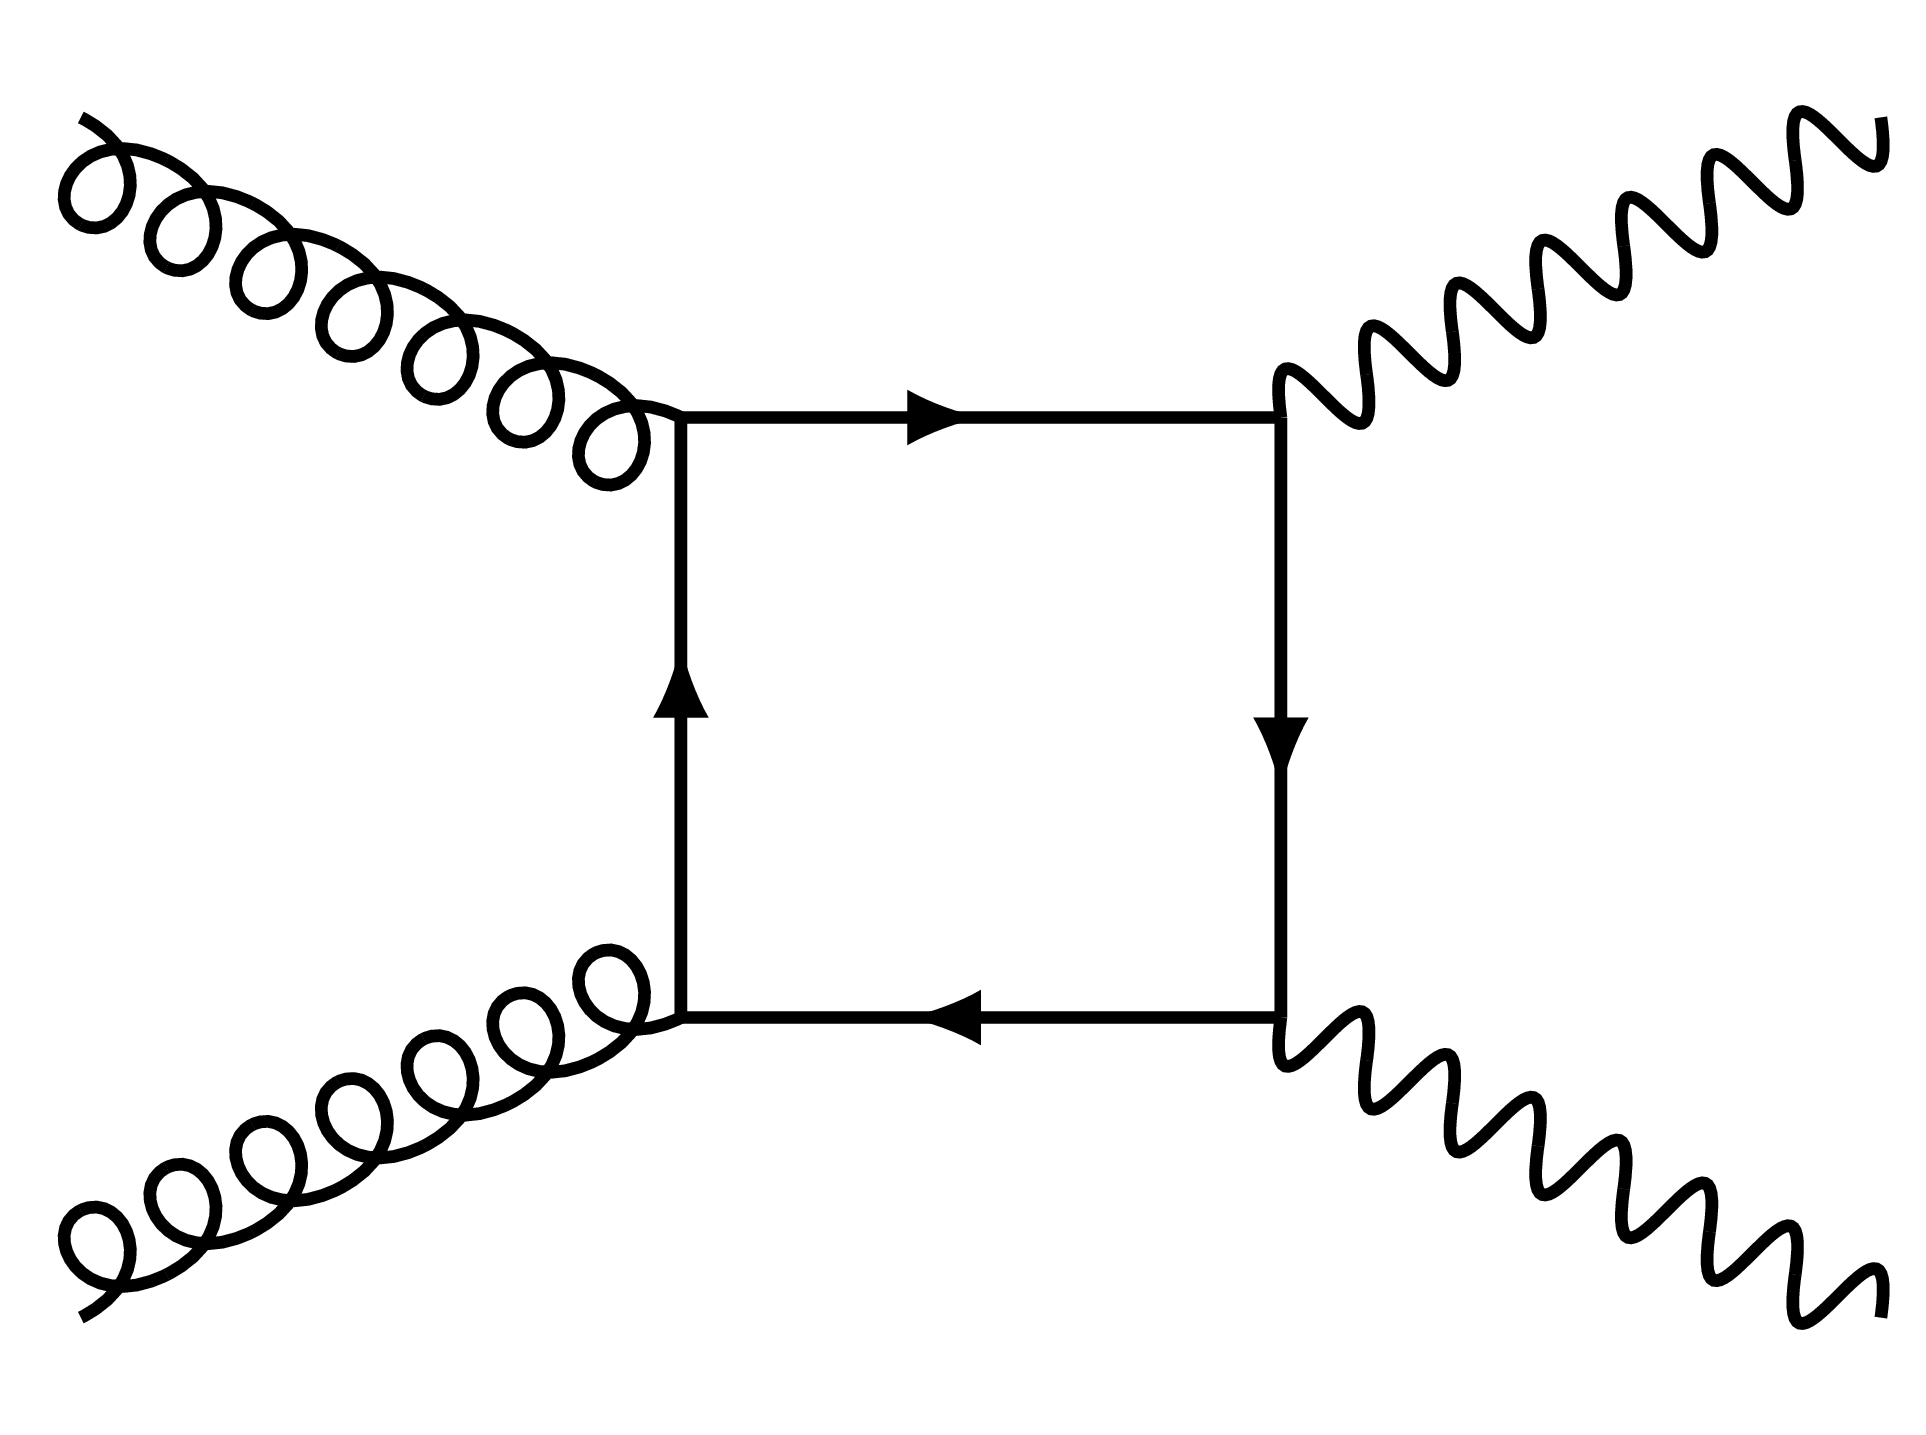
\includegraphics[scale=0.08]{ChapterAnalysis/figs/ggzz_diagram}}
	\label{fig:processes_feynman}
	\source{The AUTHOR, 2018.}
\end{figure}

%======================================================================================
\chapter{The LHC and the CMS Experiment}
%======================================================================================

\section{The Accelerators at CERN}
The CERN (\textit{European Organization for Nuclear Research}) it is a scientific complex created in 1954 and designed mainly for Particle Physics research. Its name derives from the original French acronym \textit{Conseil Européen pour la Recherche Nucléaire}, which was proposed by the funding group at 1952, aiming to create an international organization for research in fundamental Physics\footnote{Back to that time, only physicists from Nuclear Physics integrated the group, what justifies its name.}. The research lines developed nowadays at CERN goes far beyond the atomic nucleon and the group of scientists associated to it, is very diversified. The main instrumentation used at CERN are the particle accelerators and their associated detectors, which allow the scientists to access informations about the Physics in the very small world. The biggest of those accelerators is the LHC (\textit{Large Hadron Collider}) which started to be build in 1994 and was activated for the first time in September of 2008. On its first official operation phase for data collection, period from 2011 to 2013, the LHC achieved 7 and 8TeV of energy, resulting in a integrated luminosity of $\mathcal{L} = 5.051$ and $19.712~fb^{-1}$, respectivamente \cite{bib:web-cern}.

The LHC it is a hadronic collider - collides protons and lead ions (Pb) - projected by CERN to operate in a energy up to $\sqrt{s}=14$TeV in the center of mass (frame in which the total momentum of the colliding particles is null). The main motivation for its construction is the elucidation of the nature of the Electroweak Symmetry breaking (EWSB). Also, though the SM has been consistent so far with the observations, it is an effective theory. The LHC allows the test of the present theories in such way never done before. The conditions (energy density and temperature, for instance) created during the collisions are estimated to be similar to the ones existing few moments after the so called Big Bang \cite{bib:lhc-guide}. Added to this, there is the possibility to observe process related to Dark Matter, including mechanisms involving Higgs decays, for instance. 


The hadronic colliders have an increased potential to discover new particles, since they make the collisions in a range of energy (since the partons inside the protons can carry different fractions of the proton total energy). Also, the energy in the collision is higher than in a linear collider since both colliding objects are moving against each other ($E = E_{beam1} + E_{beam2}$). Another advantage is that, the protons are relatively heaviest and loss less energy while being accelerated in an intense magnetic field \cite{bib:Nature-448-2017}.

The LHC was constructed in a tunnel of $\sim$27~km. Such tunnel is located at 100~m underground and is located in the frontiers between France and Switzerland. The accelerator is approximately circular, being composed by eight main arcs in which there are 154 magnetic dipoles used to keep the particle beams in the curve trajectory. Each arc has an internal structure (Fig.~\ref{fig:lhc_cs}) divided into layers: the inner layer, which supports the beam pipes and magnetic dipoles, is constituted of iron and the outer layers are used to create a high vacuum region, being coated by a radiation and thermic shielding. Such configuration enhances the magnetic field and the system cooling made with liquid He inside the tube. The particle acceleration is done by eight (for each beam) super-conductive radio-frequency cavities disposed along the arcs, which outputs up to 2~MV at 400~MHz. Tab.~\ref{tab:lhc_parameters} shows some parameters of the LHC operation.

\begin{table}[htbp]{15cm}
\caption{Some parameters of the LHC.}
\begin{tabular}{p{10cm}p{4cm}}
\hline \hline
Parameter									&	Value					    \\
\hline
Exact circumference						    &	26 659 m					\\
Dipoles operation temperature 			    &	1.9 K (-271.3$^{\circ}$C)	\\
Number of magnets                           &	9593						\\
Number of main dipoles          			&	1232						\\
Number of main quadrupoles                  &	392							\\
Number of RF cavities (per beam)			&	8        					\\
Dipoles maximum magnetic field  			&	8.33 T						\\
Minimum distance between the bunches 		&	$\sim$7 m					\\
Projected Luminosity 						&	$10^{34}$ cm$^{-2}s^{-1}$	\\
Bunches per beam 					        &	2808						\\
Protons per bunch (at the beginning)        &	$1.1*10^{11}$				\\
Cycles in the ring by a beam    			&	11 245/s					\\
Number of collisions						&	6.e$^{8}$ /s		        \\
Energetic consuming						    &	$\sim$120 MW$^{*}$			\\
Pressure in the beam pipes          		&	10$^{-13}$ atm				\\
Beam energy        (at $\sqrt{s} = 14$ TeV)	&	350 MJ$^{**}$				\\
\hline
$^{*}$230 MW needed to supply all CERN.		&								\\
$^{**}$Equivalent to a 500 ton train at 150km/h. &					\\
\hline
\end{tabular}
\source{Adapted from \cite{bib:lhc-guide}, p. 30.}
\label{tab:lhc_parameters}
\end{table}

\begin{figure}[htbp]{15cm}
\caption{Simplified transverse section of the LHC.}
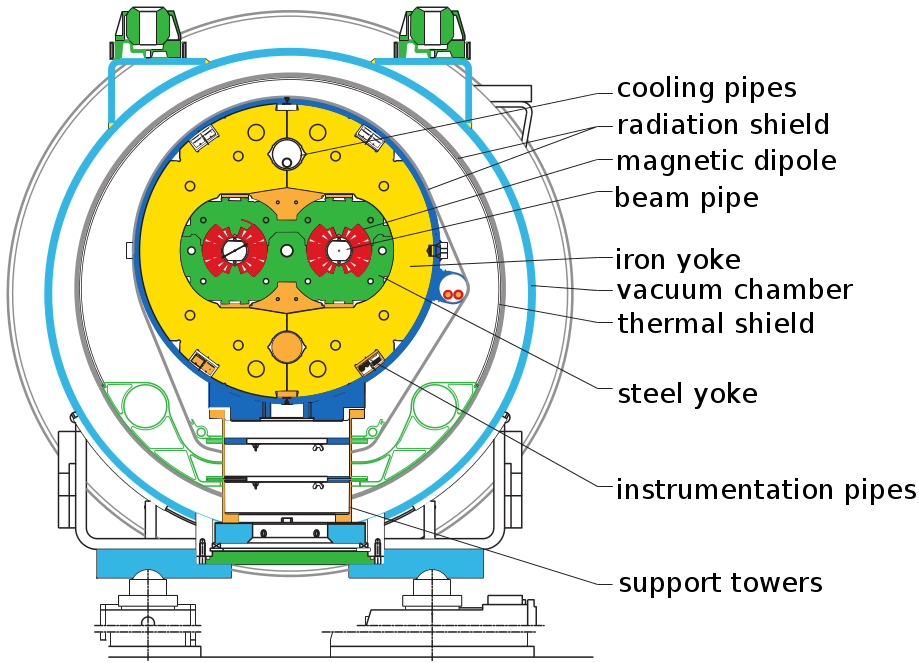
\includegraphics[scale=0.4]{ChapterCMS/figs/lhc_csp.png}
\source{Adapted from bib:Nature-448-2017, p. 286.}
\label{fig:lhc_cs}
\end{figure}

The LHC operation was structured on the already existent accelerators at CERN. These accelerators are nowadays used to make the initial particle acceleration at smaller energies. The Tab.~\ref{fig:acel_compare} summarizes the energies and velocities achieved by a proton in each accelerator up to the LHC and Fig.~\ref{fig:LHC_parts} shows an scheme of the accelerators.

\begin{table}[htbp]{15cm}
\caption{Comparison between the energy and velocity achieved by a proton in the different accelerators located at CERN.}
\begin{tabular}{p{3cm}cc}
\hline \hline
Accelerator  & Kinetic energy (K)   & Velocity ($\%$c)	    \\
\hline
Linac 2		 & 50 MeV				& 31.4					\\
PS Booster	 & 1.4 GeV				& 91.6					\\
PS			 & 25 GeV				& 99.93 				\\
SPS			 & 450 GeV				& 99.9998				\\
LHC			 & 7 TeV				& 99.9999991			\\
\hline \hline
\end{tabular}
\source{Refference \cite{bib:lhc-guide}, p. 5.}
\label{fig:acel_compare}
\end{table}

At the LHC there are four main experiments (big detectors): ALICE (\textit{A Large Ion Collider Experiment}), ATLAS (\textit{A Toroidal LHC Apparatus}), CMS (\textit{Compact Muon Solenoid}), LCHb (\textit{Large Hadron Collider beauty}). These experiments are located on the beams collision points and each of them have a complex computing system, which the main frame is called Trigger system. The Trigger is responsible to combine the information coming from the sub-detectors in each experiment and identify the particles in a fast way in order to decide if a given event is interesting to be stored and further processed (in a more refined way). Such system is very important since, at 14TeVm the bunches composing the beams are spaced by 25~ns and generates $\sim$4.e$^{7}$ crossings every second, waht can lead up to $\sim$1~G events/s \cite{bib:JINST-3-362-2008, bib:lhc-guide}. In fact, there will be upgrades on this system for future collision scenarios as it is discussed at Appendix~\ref{app:cmsl1tt}.

\begin{figure}[htbp]{15cm}
\caption{Accelerators composing the LHC at CERN.}
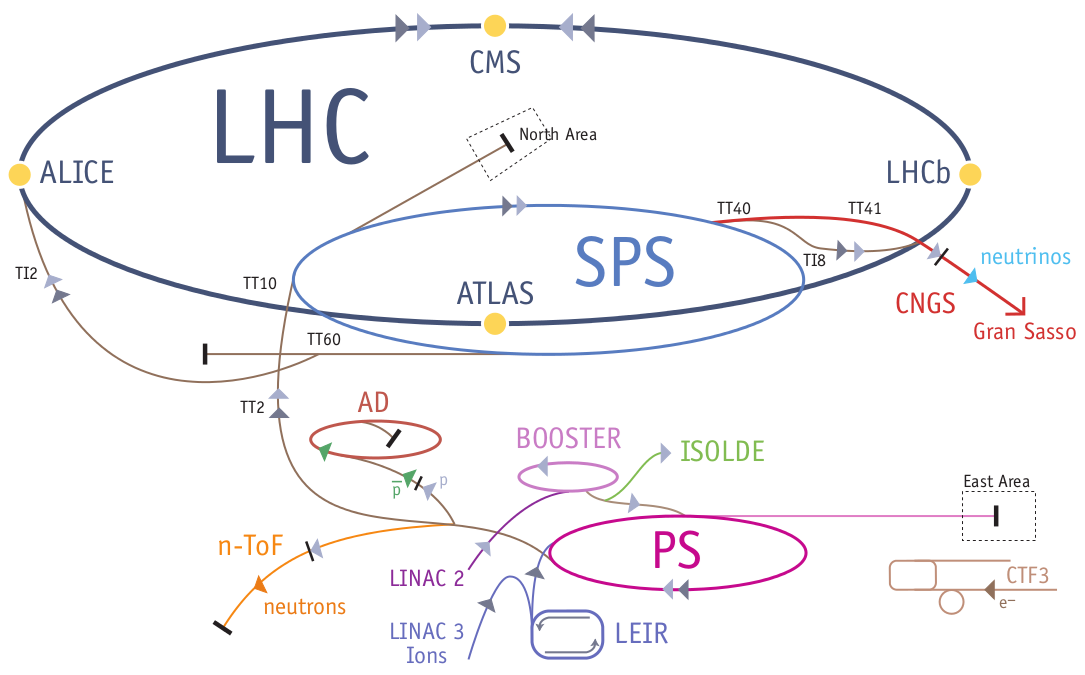
\includegraphics[scale=0.35]{ChapterCMS/figs/lhc_parts.png}
\source{Refference \cite{bib:lhc-guide}, p. 13.}
\label{fig:LHC_parts}
\end{figure}

\section{The CMS Experiment at the LHC}
The CMS is a general purpose experiment, which has similar physics goals as the ATLAS detector and both are used to look for different Physics topics. Different from ATLAS, the CMS has different detection techniques and a different magnetic system profile. Its construction is based on the traditional barrel model with two endcaps. As the name suggests, it was constructed to provide a good detection and resolution of muons. It has a giant cylindric coil made of super-conducting material, being able to generate a 3.8~T field (which is about 80 thousand times larger the the earth magnetic field). The CMS has 21~m of length, 15~m of diameter, weigh about 12500 tons and its construction cost is about R$\$$ 1,317 billions \cite{bib:lhc-guide,bib:cms-page}.

The construction of the CMS follows some requirements needed to the Physics goal in the TeV energy scale. Between them, is the good identification and resolution in the muons transverse momentum and charge, good reconstruction efficiency of the tracks from the tracker systems, good resolution in the energy deposited on the calorimeters and good resolution on the detection of missing energy transverse (MET).The coordinates system adopted in CMS has the origin in the beams collision point, while the 
\textbf{y} axis is in the vertical direction (positive to up) and the \textbf{x} axis points radially to the center of LHC circumference. Thus, the \textbf{z} axis is in the beams moving direction. The azimuthal angle $\phi$ is on the plane \textbf{xy}, being measured from the \textbf{x} axis and the polar angle $\theta$ is measured from the \textbf{z} axis. Usually, due to Lorentz invariance, the angle $\theta$ is replaced by the pseudorapidity which is defined as $\eta=-ln[tan(\theta/2)]$ \cite{bib:lhc-guide,bib:cms-page}.

The CMS experiment is composed by several sub-detectors distributed in radial layers (onion-like) around the beam pipe and each sub-detector is specialized in the detection of specif types of particles. The Fig.~\ref{fig:cms_fig1} show a sectioned view of the experiment and Fig.~\ref{fig:cms_fig2} how each type of particle interacts with each sub-detector. The main parts of the CMS are the tracker, the superconducting solenoid, the calorimeters, the muon chambers and the frontal detectors.

\begin{figure}[htbp]{16cm}
\caption{General view of CMS layers.}
\centering
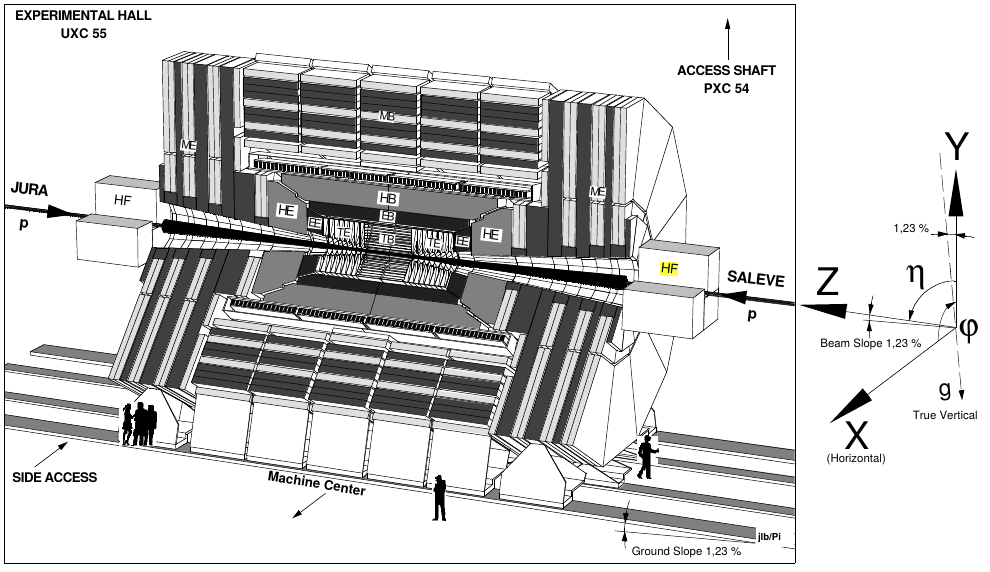
\includegraphics[scale=0.9,angle=90]{ChapterCMS/figs/cms_coordinates_system.png}
\source{Refference \cite{bib:CMS-PTDR-2006}, p. 5.}
\label{fig:cms_fig1}
\end{figure}

\begin{figure}[htbp]{16cm}
	\caption{Transverse section view showing the detection that each sub-detector does.}
	\centering
	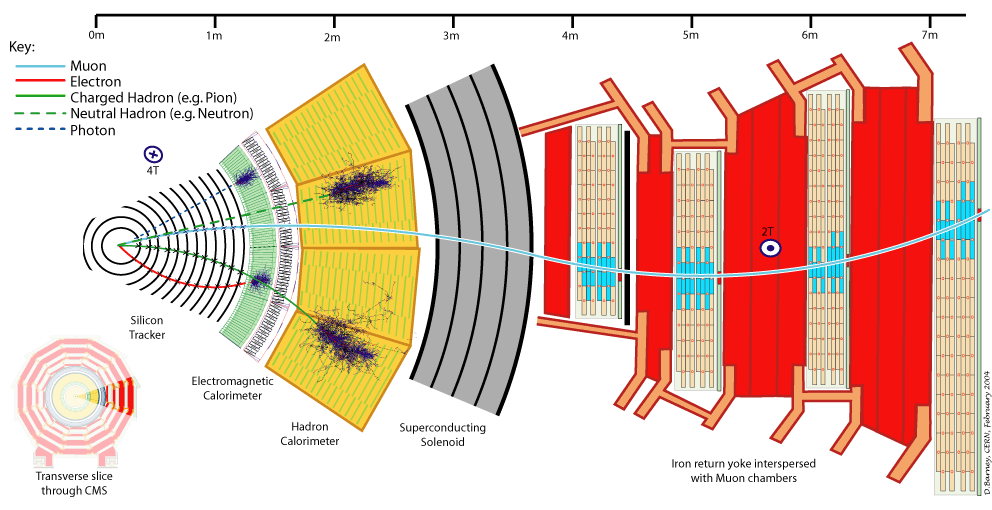
\includegraphics[scale=0.65,angle=90]{ChapterCMS/figs/cms_deteccao.png}
	\source{Refference \cite{bib:cms-page}.}
	\label{fig:cms_fig2}
\end{figure}

\subsection{The Tracker System}
The tracker system is composed by two set of detectors (Pixels and Strips) disposed radially around the beam pipe and has a total length of $\sim$5.40 m and total radius of $\sim$1.10 m. Each set presents a specific resolution but both of them detect the charged particles trajectory. The detectors used in the tracker are projected to support high radiation doses, since they are the ones closest to the collision point. Summing both set of detectors, the CMS tracker has $\sim$200 m$^{2}$ de active silicon ($SiO_{2}$). Its working principle is based on the ionization of silicon solid state sensors and in the collection of the generated charges by an electric field. This detectors stand out of the gas chambers due their higher density, which promotes absorption os higher energy particles \cite{bib:JINST-3-362-2008,bib:CMS-PTDR-2006,bib:grupen-2008}. Note, however, that this detector does not have the purpose to stop the particles, this is done by the calorimeters.

\subsubsection{The Silicon Pixels Detector}
The pixels detector comprehend the inner section of the tracker system and is projected to identify with high precision the particles trajectories in that region. It has great importance in the reconstruction of secondary vertices and in the measurement of small impact parameters, which are relevant for the identification of particles associated to heavy flavor quarks. This detector is composed by three cylindric layers, located around the beam pipe, and two discs (endcaps) located in the beam pipe transverse plane (Fig.~\ref{fig:pixel_detector}). The complete detector has 1~m$^{2}$ of silicon with 66 millions of pixels. The layers in the barrel extend for 53~cm and are disposed radially at 4.4, 7.3, 10.2~cm from the \textbf{z} axis. In the barrel there are 768 pixels with area 100$\times$150~$\mu$m$^{2}$ and disposed in a half-stair fashion way. In the discs exist 672 pixels disposed in helice and rotated by 20$^{\circ}$ around the radial direction. The pixel detector has a coverage of $|\eta| < 2.5$ and presents a resolution of about 10~$\mu$m in the \textbf{r-$\phi$} and 20~$\mu$m in the \textbf{z} direction.

\begin{figure}[htbp]{15cm}
\caption{Scheme of the pixel detector.}
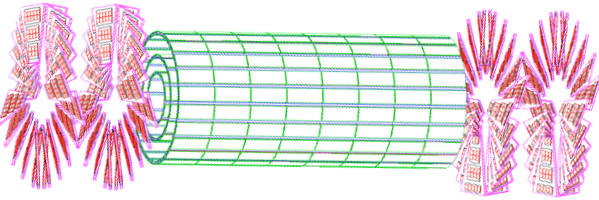
\includegraphics[scale=0.5]{ChapterCMS/figs/pixel_detector.png}
\source{bib:CMS-PTDR-2006, p. 20.}
\label{fig:pixel_detector}
\end{figure}

\subsubsection{The Silicon Strips Detector}
The silicon strips detector is the tracking system positioned around the pixels detector, being divide into two parts identified as: the Tracker Inner Barrel (TIB) and the Tracker Outer Barrel (TOB). The TIB is composed by four layers of silicon sensors with thickness of 320~$\mu$m and cover the region for $|\textbf{z}| < 65$~cm. The TOB has 6 layers, also of $SiO_2$, with average length of $|\textbf{z}| < 110$~cm. The silicon strips detector also has endcaps, which are divided into two categories: Tracker EndCaps (TEC) and Tracker Inner Discs (TID). Each TEC is composed by 9 discs which are disposed in the region $120 < |\textbf{z}| < 280$~cm and each TID is composed by 3 small discs which fill the space between the TIBs and the TECs. Both TID and TEC are organized in rings around the beam pipes and the sensors that constitute them have thickness of 320~$\mu$m (the entire TID and the 3 inner layers of the TEC) and 500~$\mu$m (remaining TEC layers). This entire detector has the length of 5.8 m and diameter of 2.6 m, containing about 10 million $SiO_{2}$ fibers. Its main designation is the track reconstruction from muons, isolated electrons and hadrons with high transverse momentum, keeping an efficiency higher than 98$\%$ in the interval $|\eta| < 2.5$.

\subsection{The Calorimeters}
A calorimeter is a system in which the particles are totally absorbed in order to measure their energy, that is, the particle is stopped. There are two types of calorimeters in the CMS: the Electromagnetic Calorimeter (ECAL) and the Hadronic Calorimeter (HCAL). The ECAL is designed to measure the energy of particles which interacts mainly electromagnetically with its material, such as electrons and photons. At high energy, the electrons loss their energy almost exclusively by the \textit{bremsstrahlung} process. The photoelectric effect and Compton also happen. The HCAL is built to measure the energy of particles which interacts through the strong and weak interactions, the case of hadrons such as pions, kaons and so on. The particles interacting with the calorimeters usually produces shower of other particles which appears from the decay of the first ones. The precision on the measurement of the energy deposited in a calorimeter is given by $\Delta E/E \propto 1/ \sqrt{E}$, and thus, the LHC can measure the particles energy with higher precision than the previous colliders.

\subsubsection{The Electromagnetic Calorimeter (ECAL)}
The ECAL is a hermetic\footnote{Capable to detect all the products of a decay by covering a big area around it (in other words, maximum coverage in the solid angle).} and homogeneous calorimeter, composed by 61200 $PbWO_4$ crystals disposed over the central barrel (EB) and by 7324 crystals in each endcap (EE). Between the properties which lead to the choice of the $PbWO_4$ as the material for the calorimeter scintillators, are the short radiation wave length ($\chi=0.89$~cm) and the short Molière radius (2.2~cm). This allowed the construction of a compact calorimeter. The Molière is a radial measurement of a cylinder, around the shower axis, which contains about 95$\%$ of its total energy, being almost independent of the energy of the incident particle. Additionally, the $PbWO_4$ scintillators are fast such that about 80$\%$ of the produced light is emitted in the interval of 25 ns \cite{bib:JINST-3-362-2008,bib:grupen-2008}.

In the barrel, the ECAL-EB covers a region of $|\eta| < 1.479$, with granularity of 1 crystal for each 1$^{\circ}$ in $\phi$. These crystals measure 23 cm in length and have faces with 22$\times$22~mm$^{2}$ (front) e 26$\times$26~mm$^{2}$ (back, where the photo-multipliers are coupled), forming a total volume of 8.14 m$^{3}$ (and weighting 67.4 tons). The $PbWO_4$ crystals are supported by a aluminum structure that keeps them spaced from each other by 0.35 mm and grouped in sub-modules. Such sub-modules are grouped in modules containing from 400 to 500 crystals. Finally, a trapezoidal structure groups four modules in so called super-modules, which form a half angular section of the barrel containing 1700 crystals (Fig.~\ref{fig:ecal}). In order to form half arc of the barrel, 18 super-modules are needed, each covering 20$^{\circ}$. On each sub-module the crystals are positioned forming a small angle with respect to the collision point in order to have coincidence between the crystal axis and the radial axises from the coordinates system.

The ECAL endcaps cover a region with $1.479 < |\eta| < 3.0$ and are installed 314 cm away from the CMS coordinates system.In that region the endcap is composed by crystals grouped in 5$\times$5 unities (called super-crystals or SCs) by a structure made of carbon fiber. Each crystal has 22 cm in length and present faces of 8.4 cm$^{2}$ (front) and 9 cm$^{2}$ (back). On each endcap, the ECAL is divided in two halves (called \textit{Dees}) which contain 3662 crystals each one. The crystals and the SCs are organized in a rectangular grid (\textbf{xy}) pointing to the origin of the CMS coordinates system. The two endcaps together comprehend a volume of 290 cm$^{3}$ and weigh 24 tons. In front the scintillators, on each endcap, there is also a shower detector (called \textit{preshower}). This detector is composed of two planes of silicon trips. The main goal of the preshower is to identify neutral pions in the region $1.653 < |\eta| < 2.6$, which allows the suppression of significant backgrounds in the $H \rightarrow \gamma\gamma$ channel \cite{bib:JINST-3-362-2008,bib:CMS-PTDR-2006}.

\begin{figure}[htbp]{15cm}
\caption{Illustration of a super-module and the entire ECAL.}
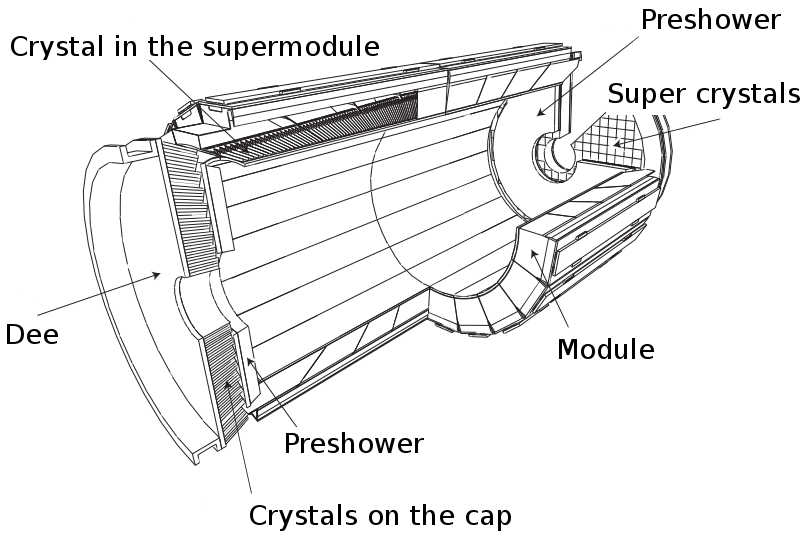
\includegraphics[scale=0.4]{ChapterCMS/figs/ecal_sched.png}
\source{Adapted from \cite{bib:JINST-3-362-2008}, p. 93 e 95.}
\label{fig:ecal}
\end{figure}

\subsubsection{The Hadronic Calorimeter (HCAL)}
Hadronic calorimeters are particularly important to the detection of jets and particles that leads to unbalance of the total energy (MET). The HCAL is installed around the ECAL in the CMS and its profile was strongly guided by the behavior of the magnetic field (since the biggest part of the HCAL is inside the solenoid). An important requirement for this detector is the enhancement on the resolution of the energy deposited on it and provide good hermecity for correct measurement of MET. This is achieved by the addition of an extra layer positioned after the solenoid, such that, the CMS HCAL can be divided in three parts: the barrels inside (HB~-~\textit{Hadron Barrel}) and outside (HO~-~\textit{Hadron Outer}) of the solenoid and, the endcaps (HE~-~\textit{Hadron Endcap}). In the barrel the HCAL goes radially from the ECAL ($R = 1.77$ m) up to the solenoid ($R = 2.95$~m).

The HB is composed by 36 towers divided in two halves with respect to the \textbf{z} axis (Fig.~\ref{fig:hcal_hb}) and covers the region with $|\eta|<1.3$. The towers are made of absorbent brass, constituted of 70$\%$ of Cu and 30$\%$ of Zn (density of 8.53~g/cm$^{3}$). There are inner and outer plates made of stainless steel that holds the towers. The complete HB towers have, then, the following structure: a steel plate with thickness of 4 cm, followed by eight brass plates with thickness of 5.1 cm and six brass plates of 5.7 cm, finishing with another steel plate with 7.5 cm. The effective HB thickness increases with the polar angle (since the particle trajectory increases) and the presence of the ECAL before the HCAL adds about 1.1~$\lambda_I$ de material \cite{bib:JINST-3-362-2008,bib:CMS-PTDR-2006}.

\begin{figure}[htbp]{15cm}
\caption{Scheme of the positions of the HB towers.}
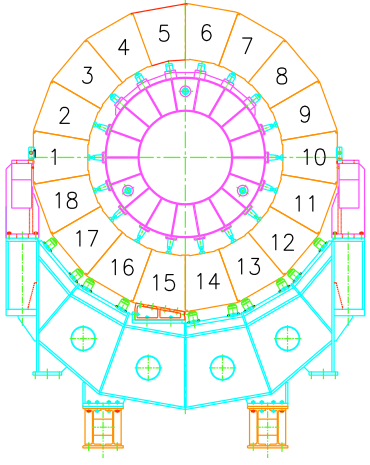
\includegraphics[scale=0.4]{ChapterCMS/figs/hcal_hb.png}
\source{Refference \cite{bib:JINST-3-362-2008}, p. 125.}
\label{fig:hcal_hb}
\end{figure}

The HE covers a region with $1.3 < |\eta| < 3$, which contains in general about 34$\%$ of the particles produced as final states. The material used on its construction was constrained by the conditions of high luminosity, the capacity of high rates counting and the high magnetic field. The chosen material for this detector was the so called C26000, which is a compound also based in brass. Each HE is coupled to the support of the muon detection system in the CMS endcaps and constitutes 36 towers positioned behind the EE (Fig.~\ref{fig:hcal_he}). The geometry used in the HE construction has the goal to reduce the discontinuities between it and the HB, besides aiming a better energy resolution of a single particle. The used brass plates have thickness of 7.9 cm and present between them plastic scintillators with $\sim$9 mm.

\begin{figure}[htbp]{15cm}
\caption{Scheme of the hadronic calorimeter in the endcaps, annexed to the muon detection system.}
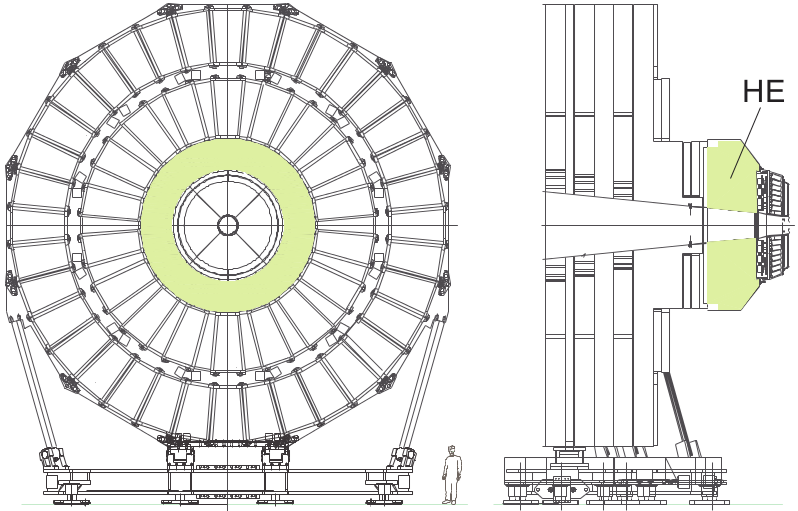
\includegraphics[scale=0.4]{ChapterCMS/figs/hcal_he.png}
\source{Refference \cite{bib:JINST-3-362-2008}, p. 131.}
\label{fig:hcal_he}
\end{figure}

Because of the radial limitation associated to the solenoid there is an additional HCAL layer positioned behind it. This is needed since the combined absorption power of the EB and the HB is not enough to fully handle the some hadronic showers. The HO covers a region of $|\eta| < 1.3$ and uses the solenoid as additional material, being able to detect showers with retarded start and thus, the reminiscent energy after the HB. The physical impact of the HO has been studied in CMS simulation. Without it one observes an excess in the ratio E$_{medida}$/E$_{incidente} < 1$ (Fig.~\ref{fig:hcal_ho_sim}), which means that, part of the total energy is lost in the reconstruction (showers "leakage" - the showers are not completely reconstructed). Such effect has a direct impact on the measure of MET and thus, the HO is an important detector for the study of processes involving strong interactions \cite{bib:JINST-3-362-2008,bib:hcal-tdr-1997}.

\begin{figure}[htbp]{15cm}
\caption{Scheme of the positions of HO in the muon detection systema and its effect on the measurement of the energy from hadronic showers.}
\subfloat[HO transverse section.]{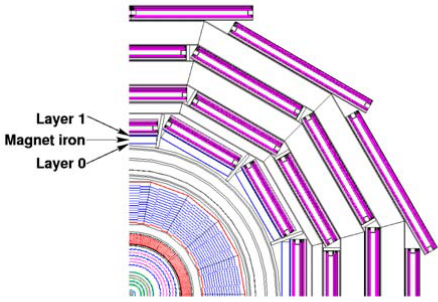
\includegraphics[scale=0.7]{ChapterCMS/figs/hcal_ho.png}} \hspace{0.5cm}
\subfloat[HO effect on the balance of energy measured in the CMS.]{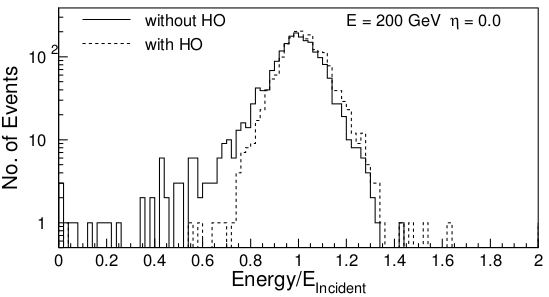
\includegraphics[scale=0.6]{ChapterCMS/figs/ho_sim.png}}
\source{Refference \cite{bib:JINST-3-362-2008}, p. 138 e 140.}
\label{fig:hcal_ho}
\label{fig:hcal_ho_sim}
\end{figure}

In the forward CMS directions there are also the HFs (Hadron Forward detectors). The HFs are calorimeters which receives very high fluxes of particles (on average 760 GeV per pp interaction is deposited into the two forward calorimeter - very small compared to the 100 GeV for the rest of CMS). Also, such energy is not uniformly distributed but increases with higher pseudorapidities. The HFs are essentially a cylindrical steel absorber structure composed by 5 mm thick grooved plates. Quartz Optical fibers are inserted in such grooves. The detector are functionally divided into two longitudinal segments. Half of the fibers run over the full depth of the absorber (165 cm) while the other half starts at a depth of 22 cm from the front of the detector. These two set of fiver have separated read out systems. Such arrangement makes it possible to distinguish between showers generated by electrons and photons (which deposit a large fraction of their energy in the first 22 cm), from the showers generated by hadrons (which produce nearly equal signals in both calorimeter segments). The HFs are located at about 11.2 m from the collision point and their inner radius is at 12.5 cm from the beam line center. The outer radius goes up to 130.0 cm. The total coverage of the HFs comprehend the region $3.0 < |\eta| < 5.0$ \cite{bib:JINST-3-362-2008,bib:hcal-tdr-1997}. Fig.~\ref{fig:hcal_hf} shows a scheme of a quadrant of the HF detector and the grooves where the optical fibers sit.

\begin{figure}[htbp]{15cm}
	\caption{An HF quadrant showing the modules of steel plates with grooves where optical fibers sit.}
	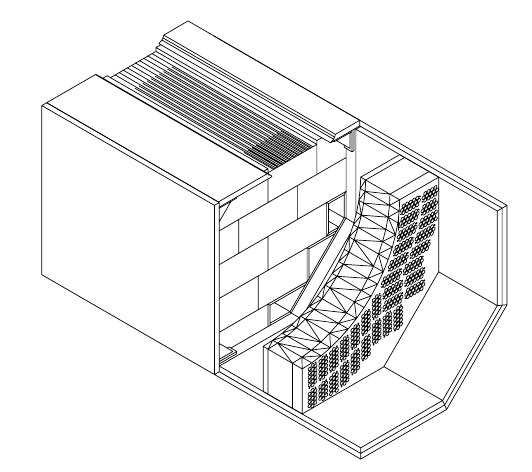
\includegraphics[scale=0.5]{ChapterCMS/figs/hcal_hf.png}
	\source{Refference \cite{bib:hcal-tdr-1997}, p. 138 e 140.}
	\label{fig:hcal_hf}
\end{figure}


\subsection{The Magnetic System}
The CMS magnetic system has the main goal the efficiency in the detection muon system and thus, also the power to bend such particles in the momentum range of $\sim$1 TeV in order to distinguish their charge. That requires a resolution of $\Delta p/p \sim10\%$ at this given momentum. For this reason, the CMS Collaboration choice was a big superconducting solenoid with 12.9 m of length, consisting of 5 rings of 5.9 m of inner radius (Fig.~\ref{fig:cms_solenoid}). Because of the huge number of wire turns need to achieve the required magnetic field, the solenoid coil is composed by 4 layers, differing from the usual one and two layers, as for Aleph and Delphi and, ZEUS and BaBar experiments, respectively. In total CMS has 2168 wire turns. The solenoid and the wires are made of NbTi and aluminum of high purity. Due to the huge magnetic field, a big part of the solenoid has structural functionality.

Because of physical reasons the radial extension of the solenoid is relatively small ($\Delta R/R \sim 0.1$) but even so, its mass is about 220 tons and it can holds up to 2.6 GJ of energy. In order to keep the solenoid superconducting a huge cryogenic system is needed. This system was constructed with a cooling capacity of 800 W at 4.45 K and 4500 W between 60-80 K and, simultaneously for a liquefaction capacity of 4 g/s. Associated to it, there is also a vacuum system capable of produce good isolation for a volume of 40 m$^{3}$. In order to assure the return of the magnetic field generated by the solenoid, a big structure made of iron (\textit{yoke}) is used in the external region around the solenoid. Such structure is composed of 11 big sections: 6 discs (endcaps) and 5 cylinders (barrel region), whith masses that vary between 400 and 1920 tons. For a precise moving of such structures (during the CMS maintenances, for instance), they sit over platforms that float over air or oil (\textit{heavy-duty air pads} and \textit{grease pads}). Because of this system the alignment of the parts composing the \textit{yoke} was done in such a good way that the final accuracy was of 2 mm of difference from the ideal center (the center of the coordinates system) \cite{bib:JINST-3-362-2008}.

\begin{figure}[htbp]{15cm}
\caption{The CMS magnetic system.}
\subfloat[Scheme of the CMS solenoid.]{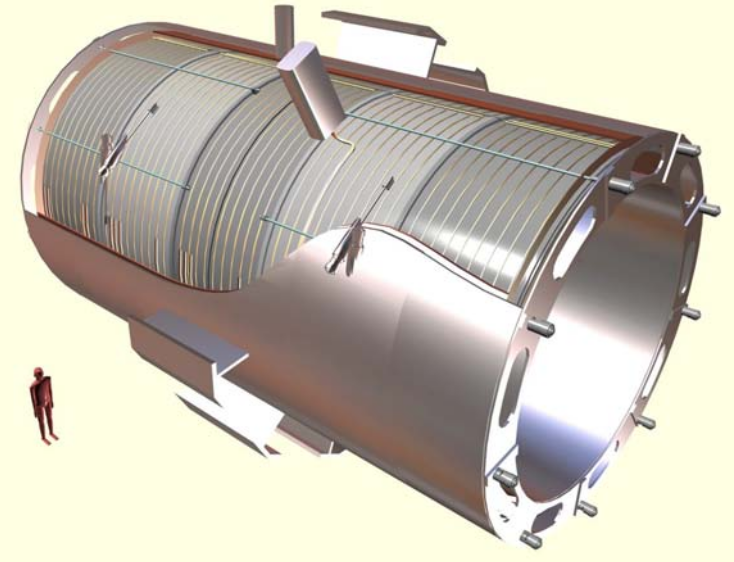
\includegraphics[scale=0.5]{ChapterCMS/figs/solenoid.png}}\quad
\subfloat[Mapping of the magnetic field created by the solenoid.]{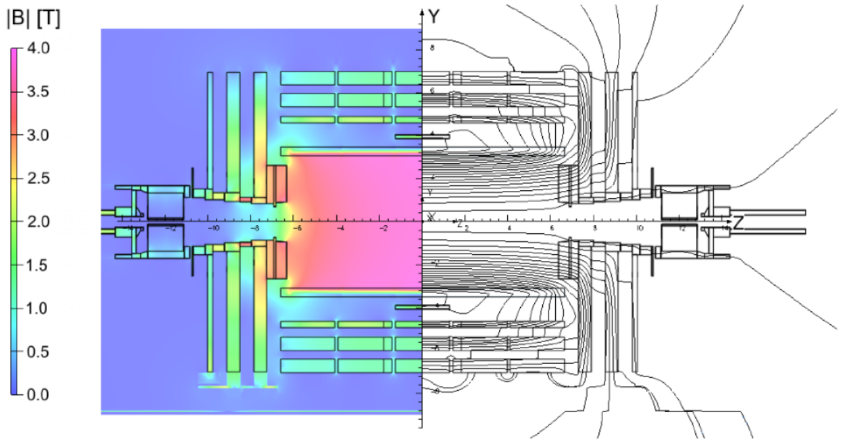
\includegraphics[scale=0.65]{ChapterCMS/figs/cms_magnetic_field_map}}
\source{Refference \cite{bib:JINST-3-362-2008} p. 7 and \cite{} p. 30.}
\label{fig:cms_solenoid}
\end{figure}

\subsection{The Muon Chambers}
This is the last and outermost set of detectors in the CMS experiment. It is constituted of 4 radial stations inserted in cavities of the \textit{yoke} and is responsible for identify and measure the transverse momentum of muons. The muon chambers are divided in three categories: the drift tube chambers (DTCs), the Cathode Strip Chambers (CSCs) and the Resistive Plate Chambers (RPCs). The DTCs are located in the barrel region, while the CSCs in the endcaps and the RPCs are installed in both barrel and endcaps. Such detectors covers the region of $0 < |\eta| < 2.4$. In the barrel the DTs cover $0 < |\eta| < 1.3$ while in the endcaps the CSCs cover $0.9 < |\eta| < 2.4$. The measurement of the muons transverse momentum using only the muon chambers is determined essentially by the curvature angle of the muons coming out of the solenoid and is not efficient as the tracker system. However, the combination of the tracker with the muon chambers can increases the resolution on the transverse momentum measurement by a factor of up to 10x (Fig.~\ref{fig:preso_detectors}) \cite{bib:CMS-PTDR-2006,bib:CMS-MSTDR-1997}.

\begin{figure}[htbp]{16cm}
\caption{Comparison of the resolution on the muon transverse momentum measurement obtained by using the muon chambers and the tracker separated and combined, left. Scheme of the muon chambers position in the CMS, right}
\centering
\subfloat[Resolutions on the measruement of the muons transverse momentum.]{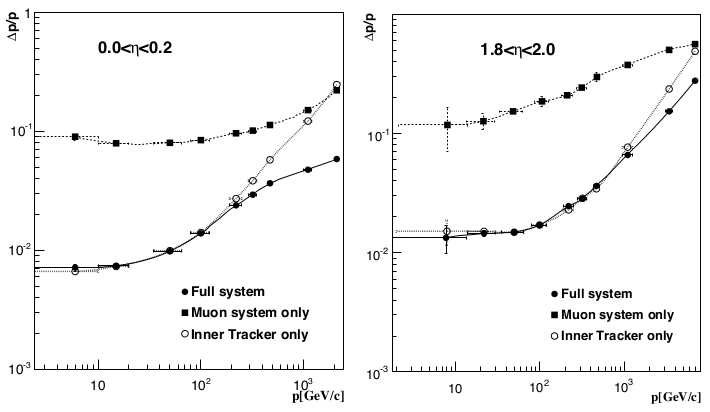
\includegraphics[scale=0.6]{ChapterCMS/figs/pmu_reso.png}}\\
\subfloat[Location of the muon chambers in a section of the CMS detector.]{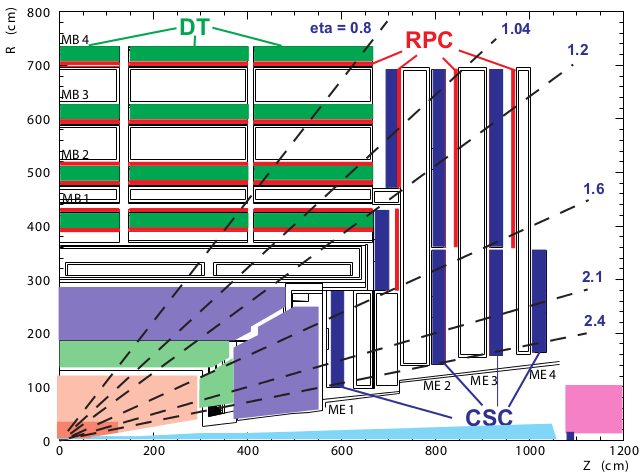
\includegraphics[scale=0.6]{ChapterCMS/figs/sist_muon_position.png}}
\source{Refference \cite{bib:CMS-PTDR-2006}, p. 11 and 12.}
\label{fig:preso_detectors}
\end{figure}

In the CMS barrel region, the muon chambers are composed by 4 stations that form concentric cylinders positioned radially at 4.0, 4.9, 5.9 and 7.0 m of the beam line center (totalizing 250 chambers). The geometry of the \textit{yoke} presents 12 sectors covering 30$^{\circ}$ in \textbf{$\phi$} and the chambers are disposed in such a way that a high momentum muon produced close to the borders of adjacent sectors crosses at least 3 or 4 chambers. There are 12 chambers in each of the 3 inner stations, while in the fourth station, the sectors above and below (hemispherically) hold 2 chambers. Each station was designed to produce a spacial vector associated to the muons with a precision em \textbf{$\phi$} better than 100 $\mu$m. The muon chambers in the endcaps is constituted of 468 CSCs in trapezoidal shape and are superposed between each other, covering the full azimuthal region (orthogonal to the beam axis). The chambers in that region has thickness of 60-10 cm, and each one covers about 10$^{\circ}$ (radially outer chambers) and 20$^{\circ}$ (radially inner chambers). All RPCs installed in the endcaps cover 20$^{\circ}$.

Although there are structural differences between the technologies used in each type of chamber, all of them work in similar way (cathode-anode principle). The DTCs are made of tubes containing gas ($Ar+CO_2$) in which there is a conducting wire Fig.~\ref{fig:sist_muon_detectors}(a). A potential difference created between the tube and the wire creates electric field such that, any charged particle crossing the tube ionizes the gas and produces a bunch of electrons (which can produce even more electrons - avalanche process) that are drifted to the wire and produces an excess of current in the detector (the signal). The distance between the particle and the wire is a function of the velocity and the time associated to the electrons in order to achieve the wire. Each DTC is composed of 12 layers of aluminum organized in 3 groups of 4, containing up to 60 tubes each one. Each layer measures in average 2$\times$2.5~m$^{2}$ and each tube is 4 cm wide. The CSCs consist of wires perpendicularly positioned to cooper fibers inserted in a gas Fig.~\ref{fig:sist_muon_detectors}(c). The difference from the DTCs are basically the higher resolution due to the use of cathodes in strip shape, which allows higher precision on the estimation of the electrons avalanche position. The RPCs are detectors composed by two parallel plates made of a plastic material with high electric resistivity and separated by gas Fig.~\ref{fig:sist_muon_detectors}(b). The plates are transparent to the electrons generated in the ionization process and those are collected by metallic fibers located after the plates. RPCs are detectors that combine a good spatial and temporal (1 ns) resolution and, because of that they are used to trigger the presence of particles in the muon detection system \cite{bib:CMS-PTDR-2006,bib:CMS-MSTDR-1997,bib:grupen-2008}.

\begin{figure}[htbp]{16cm}
\caption{Types of detectors used in the muon detection system.}
\begin{multicols}{2}
\subfloat[DTC scheme.]{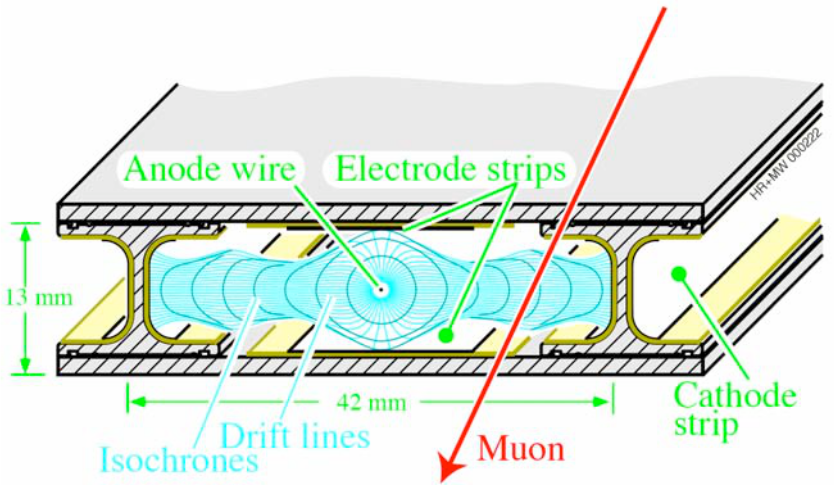
\includegraphics[scale=0.23]{ChapterCMS/figs/dtc.png}}\\
\subfloat[RPC scheme.]{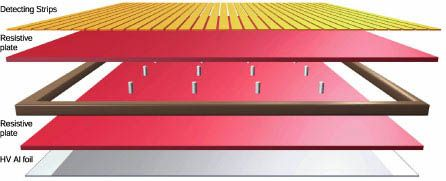
\includegraphics[scale=0.44]{ChapterCMS/figs/rpc.jpg}}\\
\subfloat[CSC scheme.]{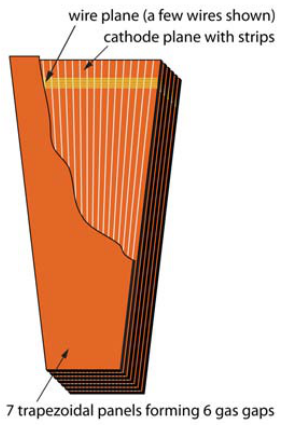
\includegraphics[height=7cm,width=5.5cm]{ChapterCMS/figs/csc.png}}
\end{multicols}
\source{Refference \cite{bib:JINST-3-362-2008}, p. 169 and \cite{bib:CMS-PTDR-2006}, p. 94.}
\label{fig:sist_muon_detectors}
\end{figure}


\subsection{The Trigger and Data Acquisition System}
The trigger system and data acquisition (TriDAS~-~\textit{Trigger and Data Acquisition System}) in a hadronic collider has a very important function, since, both the collision rates and the amount of data produced are much larger than the speed and size which can be handled. At the LHC, about 1 MB of data can be produced every crossing of the proton bunches. In such way a system that reduces the amount of data at the moment of the collision is needed. Much of what is produced in the LHC is already known Physics and very efficient filters need to be applied in order to store the Physics potentially new. Since the event rate is very high ($\mathcal{O}(10^{6})$), the filtering is divided into two stages: the level-1 trigger (L1T) and the high level trigger (HLT) \cite{bib:JINST-3-362-2008,bib:CMS-DAS-TDR-2002}. 

The L1T is composed by custom programmed hardware in (or very close to) the sub-detectors and is designed to reduce the event rate to 100 kHz. This trigger can be divide into local, regional and global components, which use informations coming from calorimeters and muon chambers to identify and organize specific objects (\textit{trigger object} - such as the EG candidates) according to their energy/momentum and the quality of such informations (which constitutes the confidence level). In 2016 there was a list (L1 trigger menu) of about 200 requirements (L1 seeds), which constitute specifications that an event should satisfy. In order to be forward for further analysis, an event has to fire the L1 seeds. If that happens then the event is sent to the next level, the HLT \cite{bib:JINST-3-362-2008,bib:CMS-DAS-TDR-2002}.

The HLT is a more complex filter based on pure software. It filters the events using a set of algorithms running on a computer farm. These algorithms are a simplified version of the algorithms used for event offline reconstruction. The HLT is designed to reduce the event rate to 100 Hz. In order to be stored an event needs to satisfy at least one of the HLT requirements (trigger paths). When that happens the event is marked for permanent storage and it is transferred to the CERN T0. Once an event is triggered by the HLT and stored in the CERN T0 it follows to the full event reconstruction. This processing is done offline (no time constraints) using the complete resolution and full information of the CMS sub-detectors and, takes at least 48h to be complete. After that, the event is ready for Physics analysis \cite{bib:JINST-3-362-2008,bib:CMS-DAS-TDR-2002}.
%%==========================================================================
\chapter{Data and Monte Carlo Samples}
\label{sec:datasets}
%%==========================================================================
\section{Data}
The data samples used in this analysis were recorded during 2016 and correspond to 35.9fb$^{-1}$ of certified data (JSON\footnote{The JSON file contains the official runs and luminosity section which should be consider when processing the datasets for a physics analysis.}: {\footnotesize Cert\_271036-284044\_13TeV\_23Sep2016ReReco\_Collisions16\_JSON.txt}).
The list of datasets is in Tab.~\ref{tab:datasets_list} along with the integrated luminosity. The analysis relies on five different primary datasets (PDs), DoubleEG, DoubleMuon, MuEG, SingleElectron, and SingleMuon, each of them combines a certain collections of HLT paths. In order to avoid duplicate events from different PDs, the events are taken:

\begin{itemize}
	\item from DoubleEG if they pass the diElectron or triElectron triggers;
	\item from DoubleMuon if they pass the diMuon or triMuon triggers and fail the diEle and triEle triggers;
	\item from MuEG if they pass the MuEle or MuDiEle or DiMuEle triggers and fail the diEle, triEle, diMuon and triMuon triggers;
	\item from SingleElectron if they pass the singleElectron trigger and fail all the triggers above;
	\item from SingleMuon if they pass the singleMuon trigger and fail all the triggers above.
\end{itemize}

The High Level Trigger (HLT) paths used are listed in Tab.~\ref{tab:hlt_triggers} together with their L1 seed, prescale value and the associated PD. The trigger efficiency measured using $4l$ events is found to be larger than $99\%$ for each of the three final states \cite{bib:CMS-AN-16-328}. 

\begin{table}[htbp]{15cm}
	\caption{Datasets used in the analysis.}
	\footnotesize
	\centering
	\begin{tabular}{c|c|c}
		\hline
		\rowcolor{light_gray}
		Run range & Datasets & Integ. luminosity\\
		\hline
		& Global Tag: 80X\_dataRun2\_2016SeptRepro\_v7 &\\
		\hline 
        & /DoubleMuon/Run2016B-03Feb2017\_ver2-v2/MINIAOD &\\
		& /DoubleEG/Run2016B-03Feb2017\_ver2-v2/MINIAOD	&\\
		273150-275376 & /MuonEG/Run2016B-03Feb2017\_ver2-v2/MINIAOD	& 5.892 fb$^{−1}$\\
		& /SingleMuon/Run2016B-03Feb2017\_ver2-v2/MINIAOD &\\
		& /SingleElectron/Run2016B-03Feb2017\_ver2-v2/MINIAOD &\\
		\hline
		& /DoubleMuon/Run2016C-03Feb2017-v1/MINIAOD &\\
		& /DoubleEG/Run2016C-03Feb2017-v1/MINIAOD &\\
		275656-276283 & /MuonEG/Run2016C-03Feb2017-v1/MINIAOD & 2.646 fb$^{-1}$\\
		& /SingleMuon/Run2016C-03Feb2017-v1/MINIAOD &\\
		& /SingleElectron/Run2016C-03Feb2017-v1/MINIAOD &\\
		\hline
		& /DoubleMuon/Run2016D-03Feb2017-v1/MINIAOD &\\
		& /DoubleEG/Run2016D-03Feb2017-v1/MINIAOD &\\
		276315-276811 & /MuonEG/Run2016D-03Feb2017-v1/MINIAOD & 4.353 fb$^{-1}$\\
		& /SingleMuon/Run2016D-03Feb2017-v1/MINIAOD &\\
		& /SingleElectron/Run2016D-03Feb2017-v1/MINIAOD &\\
		\hline
		& /DoubleMuon/Run2016E-03Feb2017-v1/MINIAOD &\\
		& /DoubleEG/Run2016E-03Feb2017-v1/MINIAOD &\\
		276831-277420 & /MuonEG/Run2016E-03Feb2017-v1/MINIAOD & 4.117 fb$^{-1}$\\
		& /SingleMuon/Run2016E-03Feb2017-v1/MINIAOD &\\
		& /SingleElectron/Run2016E-03Feb2017-v1/MINIAOD &\\
		\hline
		& /DoubleMuon/Run2016F-03Feb2017-v1/MINIAOD &\\
		& /DoubleEG/Run2016F-03Feb2017-v1/MINIAOD &\\
		277932-278808 & /MuonEG/Run2016F-03Feb2017-v1/MINIAOD & 3.186 fb$^{-1}$\\
		& /SingleMuon/Run2016F-03Feb2017-v1/MINIAOD &\\
		& /SingleElectron/Run2016F-03Feb2017-v1/MINIAOD &\\
		\hline
		& /DoubleMuon/Run2016G-03Feb2017-v1/MINIAOD &\\
		& /DoubleEG/Run2016G-03Feb2017-v1/MINIAOD &\\
		278820-280385 & /MuonEG/Run2016G-03Feb2017-v1/MINIAOD & 7.721 fb$^{-1}$\\
		& /SingleMuon/Run2016G-03Feb2017-v1/MINIAOD &\\
		& /SingleElectron/Run2016G-03Feb2017-v1/MINIAOD &\\
		\hline
		& Global Tag: 80X\_dataRun2\_Prompt\_v16 &\\
		\hline
		& /DoubleMuon/Run2016H-03Feb2017\_ver2-v1/MINIAOD
		&\\
		& /DoubleEG/Run2016H-03Feb2017\_ver2-v1/MINIAOD
		&\\
		& /MuonEG/Run2016H-03Feb2017\_ver2-v1/MINIAOD
		&\\
		& /SingleMuon/Run2016H-03Feb2017\_ver2-v1/MINIAOD
		&\\
		281207-284068 & /SingleElectron/Run2016H-03Feb2017\_ver2-v1/MINIAOD
		& 8.857 fb$^{-1}$\\
		& /DoubleMuon/Run2016H-03Feb2017\_ver3-v1/MINIAOD
		&\\
		& /DoubleEG/Run2016H-03Feb2017\_ver3-v1/MINIAOD
		&\\ 
		& /MuonEG/Run2016H-03Feb2017\_ver3-v1/MINIAOD
		&\\
		& /SingleMuon/Run2016H-03Feb2017\_ver3-v1/MINIAOD
		&\\
		& /SingleElectron/Run2016H-03Feb2017\_ver3-v1/MINIAOD
		&\\
		\hline
	\end{tabular}
	\source{CMS COLLABORATION, 2016, p. 12. Adapted by the author.}
	\label{tab:datasets_list}
\end{table}

\begin{table}[hbtp]{15cm}
	\caption{Trigger paths used in 2016 collision data.}
	\scriptsize
	\begin{tabular}{l|l|c|l}
		\hline
		\rowcolor{light_gray}
		HLT path & L1 seed & Prescale & Primary dataset\\
		\hline
		HLT\_Ele17\_Ele12\_CaloIdL\_TrackIdL\_IsoVL\_DZ & L1\_DoubleEG\_15\_10 & 1 & DoubleEG\\
		HLT\_Ele23\_Ele12\_CaloIdL\_TrackIdL\_IsoVL\_DZ & L1\_DoubleEG\_22\_10 & 1 & DoubleEG\\
		HLT\_DoubleEle33\_CaloIdL\_GsfTrkIdVL & (Multiple) & 1 & DoubleEG\\
		HLT\_Ele16\_Ele12\_Ele8\_CaloIdL\_TrackIdL & L1\_TripleEG\_14\_10\_8 & 1 & DoubleEG\\
		HLT\_Mu17\_TrkIsoVVL\_Mu8\_TrkIsoVVL & L1\_DoubleMu\_11\_4 & 1 & DoubleMuon\\
		HLT\_Mu17\_TrkIsoVVL\_TkMu8\_TrkIsoVVL & L1\_DoubleMu\_11\_4 & 1 & DoubleMuon\\
		HLT\_TripleMu\_12\_10\_5 & L1\_TripleMu\_5\_5\_3 & 1 & DoubleMuon\\
		HLT\_Mu8\_TrkIsoVVL\_Ele17\_CaloIdL\_TrackIdL\_IsoVL & L1\_Mu5\_EG15 & 1 & MuonEG\\
		HLT\_Mu8\_TrkIsoVVL\_Ele23\_CaloIdL\_TrackIdL\_IsoVL & L1\_Mu5\_EG20 & 1 & MuonEG\\
		HLT\_Mu17\_TrkIsoVVL\_Ele12\_CaloIdL\_TrackIdL\_IsoVL & L1\_Mu12\_EG10 & 1 & MuonEG\\
		HLT\_Mu23\_TrkIsoVVL\_Ele12\_CaloIdL\_TrackIdL\_IsoVL & L1\_Mu20\_EG10 & 1 & MuonEG\\
		HLT\_Mu23\_TrkIsoVVL\_Ele8\_CaloIdL\_TrackIdL\_IsoVL & L1\_SingleMu* & 1 & MuonEG\\
		HLT\_Mu8\_DiEle12\_CaloIdL\_TrackIdL & L1\_Mu6\_DoubleEG10 & 1 & MuonEG\\
		HLT\_DiMu9\_Ele9\_CaloIdL\_TrackIdL & L1\_DoubleMu7\_EG7 & 1 & MuonEG\\
		HLT\_Ele25\_eta2p1\_WPTight & L1\_SingleEG* & 1 & SingleElectron\\
		HLT\_Ele27\_WPTight & L1\_SingleEG* & 1 & SingleElectron\\
		HLT\_Ele27\_eta2p1\_WPLoose\_Gsf & L1\_SingleEG* & 1 & SingleElectron\\
		HLT\_IsoMu20 OR HLT\_IsoTkMu20 & L1\_SingleMu* & 1 & SingleMuon\\
		HLT\_IsoMu22 OR HLT\_IsoTkMu22 & L1\_SingleMu* & 1 & SingleMuon\\
		\hline
	\end{tabular}
	\source{CMS COLLABORATION, 2016, p. 13.}
	\label{tab:hlt_triggers}
\end{table}

\section{Simulated Samples}
In this analysis Higgs bosons produced via (VBF) are the signal, while the other production modes and SM backgrounds constitute the total background. The simulation of the SM Higgs is obtained via POWHEG V2 \cite{bib:JHEP_07_2008_060,bib:JHEP_11_2007_070} generator for the five main production modes: gluon fusion (ggH) including quark mass effects \cite{bib:JHEP_02_2012_088}, vector boson fusion (VBF) \cite{bib:JHEP_02_2010_037}, and associated production (WH, ZH, and ttH \cite{bib:PhysRev_D91_2015_9_094003}). For ggH its MiNLO HJJ extension is used, while in the case of WH and ZH the MiNLO HVJ is used \cite{bib:JHEP_10_2013_083}. Higgs boson decay into ZZ and subsequentially into four leptons is obtained via the JHUGEN generator \cite{bib:PhysRev_D81_2010_075022}. In the case of WH, ZH, and ttH, the Higgs boson is allowed to decay as $H \rightarrow ZZ \rightarrow 2l2X$ such that 4-lepton events where two leptons originate from the decay of associated Z or W bosons (or yet top quarks) are also taken into account in the simulation. The SM Higgs boson is also simulated when produced through ggH, VBF and associated production (WH, ZH, $b\bar{b}$H), while decaying as $H \rightarrow WW \rightarrow 2l2\nu$ (in the case of $b\bar{b}$H the MadGraph5 (aMC@NLO) generator is used). The parton showering and the hadronization are carried out by PYTHIA 8. All samples are generated with the NNPDF 3.0 NLO parton distribution functions (PDFs) \cite{bib:JHEP_04_2015_040}. The list of SM Higgs samples and their cross sections is shown in Tab.~\ref{tab:simulated_samples_list}.

The ZZ production via $q\bar{q}$ annihilation is generated at NLO using POWHEG V2 \cite{bib:EurPhysJ_C74_2014_1_2702} and PYTHIA 8, with the same settings as for the Higgs signal. As this simulation covers a large range of ZZ invariant masses, dynamical QCD factorization and renormalization scales have been chosen to be equal to $m_{ZZ}$.

The $gg \rightarrow ZZ$ process is simulated at LO with MCFM \cite{bib:NuclPhysProcSuppl_205_2010_10, bib:JHEP_04_2014_060}. In order to match the $gg \rightarrow H \rightarrow ZZ$ transverse momentum spectra predicted by POWHEG at NLO, the showering for MCFM samples is performed with different PYTHIA 8 settings, allowing only emissions up to the parton-level scale ("wimpy" shower).

Additional MC samples of WZ, Drell-Yan+jets, $t\bar{t}$, $t\bar{t}$V, and $VVV$ are generated using MadGraph5 either inclusively or merging several jet multiplicities. Tab.~\ref{tab:simulated_samples_list} summarizes the MC simulated samples used in this analysis. All samples are processed through GEANT4 \cite{bib:NuclInstrumMeth_A506_2003_250, bib:IEEETransNuclSci_53_2006_270} simulating the CMS detector and then, reconstructed through the official production chain. The Monte Carlo samples are also re-weighted to match the pileup distribution observed in 2016 data.

\begin{landscape}
\begin{table}[hbtp]{16cm}
	\caption{MC simulated samples and their respective cross section.}	
	\scriptsize
	\centering
	\begin{tabular}{l|l|l}
		\hline
		\rowcolor{light_gray}
		Process & Dataset Name & $\sigma . BR~(fb)$\\
		\hline
		& \hspace{2.5cm}\textbf{SM Higgs MC Samples} &\\
		\hline
		$gg \rightarrow H \rightarrow ZZ \rightarrow 4l$ & [1] GluGluHToZZTo4L\_M125\_13TeV\_powheg2\_minloHJJ\_JHUgenV6\_pythia8 & 12.180\\
		$q\bar{q} \rightarrow Hq\bar{q} \rightarrow ZZq\bar{q} \rightarrow 4lq\bar{q}$ & [1] VBF\_HToZZTo4L\_M125\_13TeV\_powheg2\_JHUgenV6\_pythia8 & 1.044\\
		$q\bar{q} \rightarrow W^{+}H \rightarrow W^{+}ZZ \rightarrow 4l+X$ & [1] WplusH\_HToZZTo4L\_M125\_13TeV\_powheg2-minlo-HWJ\_JHUgenV6\_pythia8 & 0.232\\
		$q\bar{q} \rightarrow W^{-}H \rightarrow W^{-}ZZ \rightarrow 4l+X$ & [1] WminusH\_HToZZTo4L\_M125\_13TeV\_powheg2-minlo-HWJ\_JHUgenV6\_pythia8 & 0.147\\
		$q\bar{q} \rightarrow ZH \rightarrow ZZZ \rightarrow 4l+X$ & [1] ZH\_HToZZ\_4LFilter\_M125\_13TeV\_powheg2-minlo-HZJ\_JHUgenV6\_pythia8 & 0.668\\
		$gg \rightarrow t\bar{t}H \rightarrow t\bar{t}ZZ \rightarrow 4l+X$ & [1] ttH\_HToZZ\_4LFilter\_M125\_13TeV\_powheg\_JHUgen\_pythia8 & 0.393\\
		$gg \rightarrow H \rightarrow WW \rightarrow 2l2\nu$ & [1] GluGluHToWWTo2L2Nu\_M125\_13TeV\_powheg\_JHUgen\_pythia8 & 1101.790\\
		$q\bar{q} \rightarrow Hq\bar{q} \rightarrow WWq\bar{q} \rightarrow 2l2\nu$ & [1] VBFHToWWTo2L2Nu\_M125\_13TeV\_powheg\_JHUgen\_pythia8 & 85.776\\
		$q\bar{q} \rightarrow W^{+}H \rightarrow W+WW \rightarrow l\nu2l2\nu$ & [1] HWplusJ\_HToWWTo2L2Nu\_WToLNu\_M125\_13TeV\_powheg\_pythia8 & 2.138\\
		$q\bar{q} \rightarrow W^{-}H \rightarrow W^{-}WW \rightarrow l\nu2l2\nu$ & [1] HWminusJ\_HToWWTo2L2Nu\_WToLNu\_M125\_13TeV\_powheg\_pythia8 & 1.357\\
		$q\bar{q} \rightarrow ZH \rightarrow Z WW \rightarrow 2l2l2\nu$ & [1] HZJ\_HToWWTo2L2Nu\_ZTo2L\_M125\_13TeV\_powheg\_pythia8 & 2.029\\
		$gg \rightarrow b\bar{b}H \rightarrow b\bar{b}WW \rightarrow 2l2\nu+X$ & [1] bbHToWWTo2L2Nu\_M-125\_4FS\_yb2\_13TeV\_amcatnlo & 11.068\\
		\hline
		& \hspace{2cm}\textbf{SM Backgrounds MC Samples} &\\
		\hline		
		$q\bar{q} \rightarrow ZZ \rightarrow 4l$ & [2] ZZTo4L\_13TeV\_powheg\_pythia8 & 1256.000\\
		$q\bar{q} \rightarrow ZZ \rightarrow 4l$ & [2] ZZTo4L\_13TeV-amcatnloFXFX-pythia8 & 1212.000\\
		$q\bar{q} \rightarrow ZZ \rightarrow 4l + jets (EWK)$ & [2] ZZJJTo4L\_EWK\_13TeV-madgraph-pythia8/
		 & 4.404\\
		$gg \rightarrow ZZ \rightarrow 4e$ & [2] GluGluToContinToZZTo4e\_13TeV\_MCFM701 & 1.590\\
		$gg \rightarrow ZZ \rightarrow 4\mu$ & [2] GluGluToContinToZZTo4mu\_13TeV\_MCFM701 & 1.590\\
		$gg \rightarrow ZZ \rightarrow 4\tau$ & [2] GluGluToContinToZZTo4tau\_13TeV\_MCFM701 & 1.590\\
		$gg \rightarrow ZZ \rightarrow 2e2\mu$ & [2] GluGluToContinToZZTo2e2mu\_13TeV\_MCFM701 & 3.190\\
		$gg \rightarrow ZZ \rightarrow 2e2\tau$ & [2] GluGluToContinToZZTo2e2tau\_13TeV\_MCFM701 & 3.190\\
		$gg \rightarrow ZZ \rightarrow 2\mu2\tau$ & [2] GluGluToContinToZZTo2mu2tau\_13TeV\_MCFM701 & 3.190\\
		\hline
		$Z \rightarrow ll + jets$ & [2] DYJetsToLL\_M-10to50TuneCUETP8M1\_13TeV-amcatnloFXFX-pythia8 & 6.104$e^{6}$\\
		& [2] DYJetsToLL\_M-50\_TuneCUETP8M1\_13TeV-amcatnloFXFX-pythia8 & 1.861$e^{7}$\\
		\hline
		$t\bar{t}$ & [2] TTJets\_TuneCUETP8M1\_13TeV-amcatnloFXFX-pythia8 & 815.96$e^{5}$\\
		$t\bar{t} \rightarrow 2l2\nu2b$ & [2] TTTo2L2Nu\_13TeV-powheg & 8.731$e^{4}$\\
		$WZ \rightarrow 3l\nu$ & [2] WZTo3LNu\_TuneCUETP8M1\_13TeV-powheg-pythia8 & 4430\\
		$ZZZ$ & [2] ZZZ\_TuneCUETP8M1\_13TeV-amcatnlo-pythia8 & 13.980\\
		$WWZ$ & [2] WWZ\_TuneCUETP8M1\_13TeV-amcatnlo-pythia8 & 165.100\\
		$WZZ$ & [2] WZZ\_TuneCUETP8M1\_13TeV-amcatnlo-pythia8 & 55.650\\
		$t\bar{t}W$ & [2] TTWJetsToLNu\_TuneCUETP8M1\_13TeV-amcatnloFXFX-madspin-pythia8 & 204.300\\
		$t\bar{t}Z$ & [2] TTZToLLNuNu\_M-10\_TuneCUETP8M1\_13TeV-amcatnlo-pythia8 & 252.900\\
		\hline
	\end{tabular}
	\begin{flushleft}
		[1] RunIISummer16MiniAODv2-PUMoriond17\_80X\_mcRun2\_asymptotic\_2016\_TrancheIV\_v6-v1/
		\newline
		[2] RunIISummer16MiniAODv2-PUMoriond17\_80X\_mcRun2\_asymptotic\_2016\_TrancheIV\_v6-v1/		
	\end{flushleft}
	\source{CMS COLLABORATION, 2016 p. 14 and 15. Adapted by the author.}
	\label{tab:simulated_samples_list}
\end{table}
\end{landscape}

%%==========================================================================
\chapter{Physics Objects Selections}
\label{sec:physics_objects_selections}
%%==========================================================================
The present analysis is based on the following physics objects: electrons, muons, missing transverse energy ($E_{T}^{miss}$), and jets. In the following subsections the main selection criteria for such object is presented while a detailed and complete description can be found in \cite{bib:CMS-AN-16-442,bib:CMS-AN-16-217}. The selection (reconstruction, identification and isolation) of objects is the same as in the SM $H \rightarrow ZZ \rightarrow 4l$ analysis.

\section{Electrons}
Electrons are required to have transverse momentum $p_{T}>$ 7GeV, $|\eta|<$ 2.5, and to satisfy a loose primary vertex (PV) constraint defined as $|d_{xy}|<$ 0.5cm and $|d_{z}|<$ 1cm. Such electrons are referred to as \textit{loose electrons}. The early runs in 2016 data-taking exhibit a tracking inefficiency originating from a reduced hit reconstruction efficiency in the strip detector ("HIP" effect). The resulting data-MC discrepancy is corrected using scale factors as it is done for the electron selection with efficiencies measured in data using the same tag-and-probe technique outlined later. These studies are carried out by the Electron Gamma Physics Object Group (EGM POG) and electron reconstruction (tracking) scale factors as a function of the super cluster $\eta$ are derived and used for this analysis (it was shown that the $p_{T}$ dependence of the scale factor is negligible). More details on electron reconstruction can be found in \cite{bib:JINST-10-2015-P06005}.

Reconstructed electrons are identified by means of a Gradient Boosted Decision Tree (GBDT) multivariate classifier algorithm, which exploits observables from the electromagnetic cluster, the matching between the cluster and the electron track as well as observables based exclusively on tracking measurements. The BDT has been retrained using $CMSSW\_8\_0\_X$ samples\footnote{CMSSW stands for the software used by the CMS collaboration in order to process events simulating the conditions of the CMS detector.}. The classifier is trained on a $DY$+jets MC sample for both signal and background. Tab.~\ref{tab:electron_classifier_vars} summarizes the full list of observables used as input to the classifier and Tab.~\ref{tab:bdt_minimum_score_electron} lists the cut values applied to the BDT score for the chosen working point. For the analysis, we define tight electrons as the loose electrons that pass this MVA identification working point.

\begin{table}[hbtp]{15cm}
	\caption{Overview of input variables to the electron identification classifier. Variables not used in the RunI MVA are marked with *.}	
	\footnotesize
	\centering
	\begin{tabular}{c|p{11.5cm}}
		\hline
		Observable & Observable name\\
		\hline
		Cluster shape & RMS of the energy-crystal number spectrum along $\eta$ and $\phi$; $\sigma_{i\eta i\eta}$, $\sigma_{i\sigma i\sigma}$\\
		& super cluster width along $\eta$ and $\phi$\\
		& ratio of the hadronic energy divided by the supercluster energy, H/E\\
		& circularity $(E_{5×5}−E_{5×1})/E_{5×5}$\\
		& sum of the seed and the 9 adjacent crystals divided by the supercluster energy, $R_{9}$\\
		& for Endcap training bins: energy fraction in pre-shower, $E_{PS}/E_{raw}$\\
		\hline
		Track-cluster & energy-momentum agreement $E_{tot} /p_{in}$, $E_{ele}/p_{out}$, $1/E_{tot}−1/p_{in}$\\
		matching & position matching $\Delta\eta_{in}$, $\Delta\phi_{in}$, $\Delta\eta_{seed}$\\
		\hline
		Tracking & fractional momentum loss $f_{brem}=1−p_{out}/p_{in}$\\
		& number of hits of the KF and GSF track $N_{KF}$, $N_{GSF}$ *\\
		& reduced $\chi^{2}$ of the KF and GSF track $\chi^{2}_{KF}$, $\chi^{2}_{GSF}$\\
		& number of expected but missing inner hits *\\
		& probability transform of conversion vertex fit $\chi^{2}$ *\\
		\hline
	\end{tabular}
	\source{CMS COLLABORATION, 2016, p. 16.}
	\label{tab:electron_classifier_vars}
\end{table}

\begin{table}[hbtp]{15cm}
	\caption{Minimum BDT score required for passing the electron identification.}
	\centering
	\begin{tabular}{c|c|c|c}
		\hline
		Minimum BDT score & $|\eta| < 0.8$ & $0.8 < |\eta| < 1.479$ & $|\eta| > 1.479$\\
		\hline
		$5 < p_{T} < 10 GeV$ & -0.211 & -0.396 & -0.215\\
		$p_{T} > 10 GeV$	 & -0.870 & -0.838 & -0.763\\
		\hline
	\end{tabular}
	\source{CMS COLLABORATION, 2016, p. 16.}
	\label{tab:bdt_minimum_score_electron}
\end{table}

Electrons are required to be isolated and the relative isolation is defined as

\begin{equation}
RelPFiso = \frac{\left( \sum_{charged} p_{T} + \sum_{neutral}^{corr} p_{T} \right)}{p_{T}^{lepton}}
\end{equation}

where the corrected neutral component of isolation is computed using the formula

\begin{equation}
\sum_{neutral}^{corr} p_{T} = max( \sum_{neutral}^{uncorr} p_{T} - \rho \times A_{eff}, 0 )~GeV
\end{equation}

and the mean pile-up contribution to the isolation cone is obtained by

\begin{equation}
PU = \rho \times A_{eff}
\end{equation}

where $\rho$ is the mean energy density in the event and $A_{eff}$ the effective area which is defined as the ratio between the slope of the average isolation and the slope of $\rho$ as a function of the number of vertices. The electron isolation working point was optimized in \cite{bib:CMS-AN-15-277} and was chosen as $RelPFiso(\Delta R = 0.3) < 0.35$.

Electrons in data are also corrected for features in ECAL energy scale in bins of $p_{T}$ and $|\eta|$. Corrections are calculated on a $Z \rightarrow ee$ sample to align the di-electron mass spectrum in the data to the one in simulation and to minimize the width of the distribution.

The $Z \rightarrow ee$ mass resolution in simulation is made to match data by applying a pseudo-random Gaussian smearing to electron energies, with Gaussian parameters varying in bins of $p_{T}$ and $|\eta|$. This has the effect of convolving the electron energy spectrum with a Gaussian. The electron energy scale is measured in data by fitting a Crystal-Ball function to the di-electron mass spectrum around the Z peak in the Z+jets control region.

\subsection{Electron Efficiency Measurements}
The tag-and-probe (T$\&$P) study was performed on the single electron primary datasets listed in Tab.~\ref{tab:datasets_list} using a JSON corresponding to 36.8$fb^{-1}$. More details on the tag-and-probe method can be found in \cite{bib:CMS-AN-15-277}. Tagged electrons need to satisfy the following quality requirements:

\begin{itemize}
	\item trigger matched to HLT\_Ele27\_eta2p1\_WPTight\_Gsf\_v*;
	\item $p_{T} > 30$GeV, super cluster (SC) $|\eta| < 2.1$ but on in EB-EE gap ($1.4442 < |\eta| < 1.566$);
	\item "tight" working point of the Spring16 cut-based electron ID\footnote{Spring16 stands for the set of standard cuts/selections used by the CMS collaboration for analyzing the data collected during the Spring in 2016.}.
\end{itemize}

Probe electrons only need to be reconstructed as GsfElectron. The Final State Radion (FSR) recovery algorithm used in the main analysis is used consistently throughout the efficiency measurement: the isolation is calculated after removing any FSR photon matched to the electron and the electron $p_{T}$ itself, and the di-electron invariant mass is estimated by including the FSR photons (if any). The nominal MC efficiencies are evaluated from the LO MadGraph DY sample, while the NLO systematics use the 0 and 1 jet MadGraph\_AMCatNLO sample listed in Tab.~\ref{tab:simulated_samples_list}.

In contrast to previous efficiency measurements, a template fit is used here. The $m_{ee}$ signal shape of the passing and failing probes is taken from MC and convoluted with a Gaussian. The data are then fitted with the convoluted MC template and a CMSShape (an error-function with a one-sided exponential tail). This change follows from the usage of the new T$\&$P tool developed by the EGM POG. The electron selection efficiency is measured as a function of the probe electron $p_{T}$ and $\eta$, and separately for electrons falling in the ECAL gaps. Fig.~\ref{fig:electron_selection_efficiency} shows the $p_{T}$ turn-on curves measured in data; final scale factors for the efficiencies are derived and used within the analysis. The EGM recommendations on the evaluation of tag-and-probe uncertainties for efficiency measurements are followed.

\begin{figure}[hbtp]{16cm}
	\caption{Electron selection efficiencies measured using the tag-and-probe technique.}
	\centering
	\subfloat[]{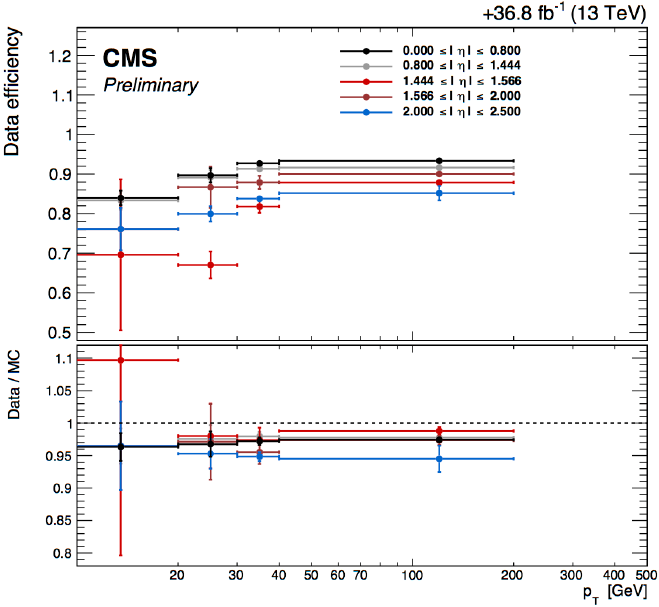
\includegraphics[scale=0.6]{ChapterAnalysis/figs/electron_selection_efficiencies_ingap}}\\
	\subfloat[]{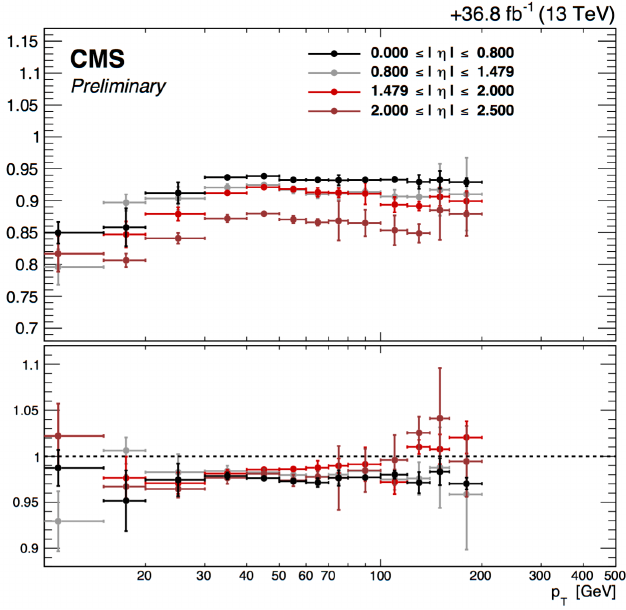
\includegraphics[scale=0.6]{ChapterAnalysis/figs/electron_selection_efficiencies_nongap}}
	\legend{(a) gap electrons; (b) non-gap electrons.}
	\source{CMS COLLABORATION, 2016, p. 18.}
	\label{fig:electron_selection_efficiency}
\end{figure}


\section{Muons}
Further details on muon reconstruction can be found in \cite{bib:CMS-AN-16-328}. Two types of selection are performed. We define \textbf{loose muons} as the muons satisfying $p_{T}>$ 5GeV, $|\eta|<$ 2.4, $d_{xy}<$ 0.5cm and $d_{z}<$ 1cm, where $d_{xy}$ and $d_{z}$ are defined with respect to the primary vertex (PV) and using the \textit{muonBestTrack}. Muons have to be reconstructed by either the \textit{GlobalMuon} or \textit{TrackerMuon} algorithm. Standalone muon tracks reconstructed only in the muon system are rejected. Muons with \textit{muonBestTrackType} == 2 (standalone) are also discarded, even if they are marked as global or tracker muons. Loose muons with $p_{T}<$ 200GeV are considered \textit{tight muons} if they also pass the PF muon ID (note that the naming convention used for these IDs differs from the muon POG naming scheme, in which the "tight ID" used here is called the "loose ID"). Loose muons with $p_{T}>$ 200GeV are considered tight muons if they pass the PF ID or the Tracker High-$p_{T}$ ID, the definition of which is shown in Tab.~\ref{tab:mu_tracker_highpTID_requirements}.

\begin{table}[hbtp]{16cm}
	\caption{The requirements for a muon to pass the tracker high-$p_{T}$ ID. Note that these are equivalent to the Muon POG high-$p_{T}$ ID with the global track requirements removed.}
	\centering
	\begin{tabular}{l|p{9cm}}
		\hline
		Plain-text description     & Technical description\\
		\hline
		Muon station matching      & Muon is matched to segments in at least two muon stations\\
		Good $p_{T}$ measurement   & $p_{T}/\sigma_{p_{T}} < 0.3$\\
		Vertex compatibility (x-y) & $d_{xy} < 2mm$\\
		Vertex compatibility (x)   & $d_{z}<5mm$\\
		Pixel hits                 & At least one pixel hit\\
		Tracker hits               & Hits in at least six tracker layers\\
		\hline
	\end{tabular}
	\source{CMS COLLABORATION, 2016, p. 18.}
	\label{tab:mu_tracker_highpTID_requirements}
\end{table}

An additional "ghost-cleaning" step is performed to deal with situations when a single muon can be incorrectly reconstructed as two or more muons:
\begin{itemize}
	\item Tracker Muons that are not Global Muons are required to be "arbitrated", i.e. associated to the segments in the outer muon detectors;
	\item If two muons are sharing 50$\%$ or more of their segments, the muon with lower quality is removed.
\end{itemize}

Muons are required to be isolated similarly as described for electrons. The pileup contribution subtraction is performed in a different way for muons. A correction $\Delta \beta = \frac{1}{2}(\sum_{PU}^{charged~had.} p_{T})$, that gives an estimate of the energy deposit from neutral particles coming from pileup vertices, is applied. The relative muon isolation is then defined as 

\begin{equation}
RelPFiso = \frac{\sum^{charged~had.} p_{T} + max(\sum^{neutral~had.} E_{T} + \sum^{photon} E_{T} - \Delta \beta, 0)}{p_{T}^{lepton}}
\end{equation}

The muon isolation was optimized in \cite{bib:CMS-AN-15-277} and the working point is chosen to be equal to the one for electrons, that is, RelPFiso$(\Delta R = 0.3)<$ 0.35.

\subsection{Muon Efficiency Measurements}
Muon efficiencies are also measured with the T$\&$P method, which is then performed on $Z \rightarrow \mu\mu$ and $J/\psi \rightarrow \mu\mu$ events in bins of $p_{T}$ and $\eta$. More details on the methodology can be found in \cite{bib:CMS-AN-15-277}. The Z sample is used to measure the muon reconstruction and identification efficiency at high $p_{T}$, and the efficiency of isolation and impact parameter at $p_{T}$. The $J/\psi$ sample is used to measure the reconstruction efficiency at low $p_{T}$ as it benefits from a better purity in such kinematic regime. Events are collected using HLT\_Mu7p5\_Track2\_Jpsi\_v* when probing the reconstruction and identification efficiency in the muon system. For probing the muon tracking efficiency HLT\_Mu7p5\_L2Mu2\_Jpsi\_v* is used.

Muon reconstruction and identification efficiency for $p_{T}>$ 20GeV have been derived by the Muon POG. The probe in this measurement are tracks reconstructed in the inner tracker, and the passing probes are those that are also reconstructed as a global or tracker muon and passing the Muon POG Loose muon identification. For low $p_{T}$ muons $J/\psi$ events have been used, with the same definitions of
"probe" and "passing probe". The systematic uncertainties are estimated by varying the analytical signal and background shape models used to fit the di-muon invariant mass. Details on the procedure can be found in \cite{bib:CMS-AN-15-277}. The efficiency and scale factors used for low $p_{T}$ muons
are the ones derived using single muon prompt-Reco dataset\footnote{These are datasets created by CMS when collecting data. They have the first reconstruction of the events in the collected data.}. The efficiencies in data and in simulation are shown in Fig.~\ref{fig:muon_reco_id_efficiency}.

\begin{figure}[hbtp]{16cm}
	\caption{Muon reconstruction and identification efficiencies.}
	\centering
	\subfloat[]{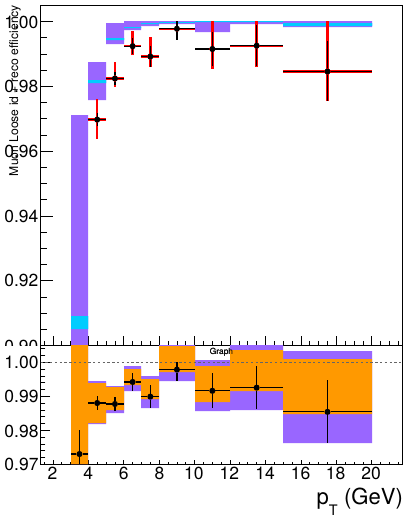
\includegraphics[scale=0.45]{ChapterAnalysis/figs/muon_reco_id_eff_barrel}}
	\quad
	\subfloat[]{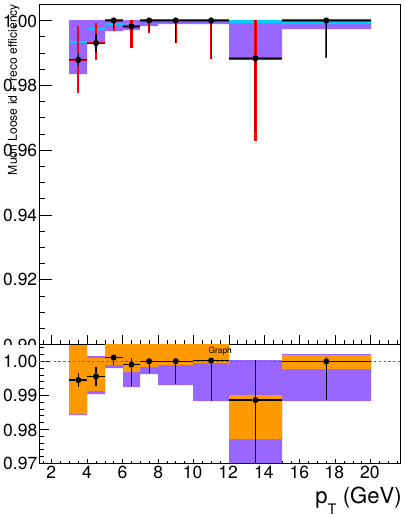
\includegraphics[scale=0.45]{ChapterAnalysis/figs/muon_reco_id_eff_endcap}}
	\quad
	\subfloat[]{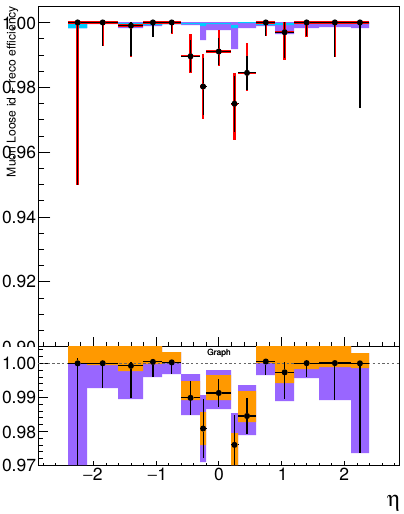
\includegraphics[scale=0.45]{ChapterAnalysis/figs/muon_reco_id_eff_eta}}
	\legend{(a) efficiency for $p_{T}<$ 20 GeV as a function of $p_{T}$ in the barrel and (b) endcaps; (c) efficiency as a function of $\eta$ for $p_{T}>$ 7 GeV. In the upper panel the cyan (black) error bars show only the statistical uncertainty and the red (violet) ones represent the total uncertainty from MC (data). In the ratio plot of the two efficiencies, the black error bars represent the statistical uncertainty, the orange ones the systematical uncertainty, and the violet ones the total uncertainty.}
	\source{CMS COLLABORATION, 2016, 20.}
	\label{fig:muon_reco_id_efficiency}
\end{figure}

The requirements for the impact parameter is studied using Z events selected with the trigger HLT\_IsoMu20\_v* or HLT\_IsoMu22\_v*. For this measurement, the probe is a muon passing the POG "loose" identification criteria, and it is considered a "passing" probe if it satisfies the $SIP_{3D}$, $d_{xy}$ and $d_{z}$ cuts\footnote{$SIP_{3D} = IP/\sigma_{IP}$ is the significance of the impact parameter (a ratio between the impact parameter in 3D - distance from collision center - and its associated uncertainty), $d_{xy}$ is the distance to the beam in the \textbf{xy} plane and $d_{z}$ is the distance in the \textbf{z} direction to the primary vertex (that is, the collision point).} of this analysis. The results are shown in Fig.~\ref{fig:muon_sip_efficiency}.

\begin{figure}[hbtp]{16cm}
	\caption{Efficiency of the muon impact parameter requirements as a function of $p_{T}$.}
	\centering
	\subfloat[]{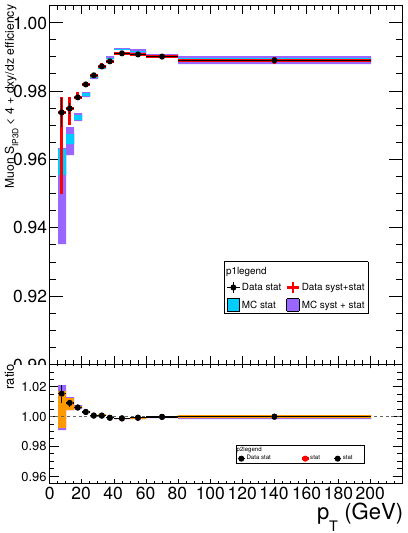
\includegraphics[scale=0.45]{ChapterAnalysis/figs/muon_sip_eff_barrel}}
	\quad
	\subfloat[]{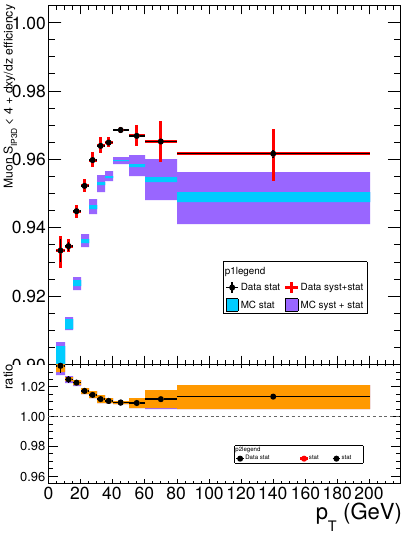
\includegraphics[scale=0.45]{ChapterAnalysis/figs/muon_sip_eff_endcap}}
	\quad
	\subfloat[]{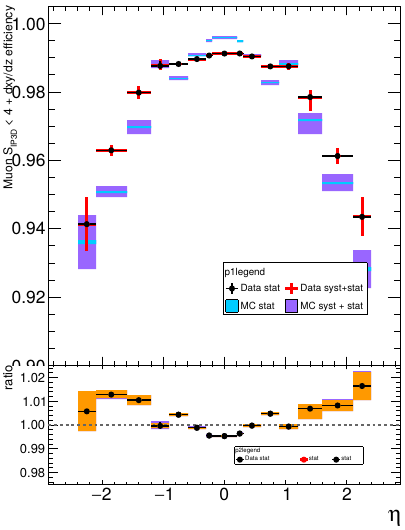
\includegraphics[scale=0.45]{ChapterAnalysis/figs/muon_sip_eff_eta}}
	\legend{(a) electrons in the barrel; (b) electrons in the endcaps; (c) as a function of $\eta$ for $p_{T}>$ 20GeV. In the upper panel the cyan (black) error bars show only the statistical uncertainty and the red (violet) ones represent the total uncertainty from MC (data). In the ratio plot the black error bars are for the statistical uncertainty, the orange ones for the systematical uncertainty and the violet ones include both uncertainties.}
	\source{CMS COLLABORATION, 2016, p. 20.}
	\label{fig:muon_sip_efficiency}
\end{figure}

The muon isolation efficiency is measured using events from the Z decay at any $p_{T}$. The events are selected with the same triggers as for the SIP study. The isolation of the muons are calculated after recovery of the FSR photons and subtracting their contribution from the isolation cone of the muons. More detailed description of the method can be found in \cite{bib:CMS-AN-16-328}. Results are shown in Fig.~\ref{fig:muon_iso_efficiency}.

\begin{figure}[hbtp]{16cm}
	\caption{Efficiency of the muon isolation requirement as a function of $p_{T}$.}
	\centering
	\subfloat[]{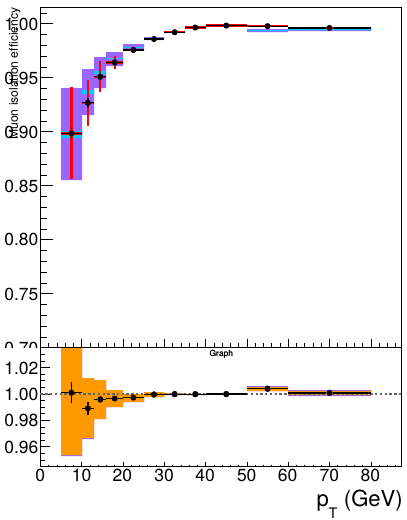
\includegraphics[scale=0.45]{ChapterAnalysis/figs/muon_iso_eff_barrel}}
	\quad
	\subfloat[]{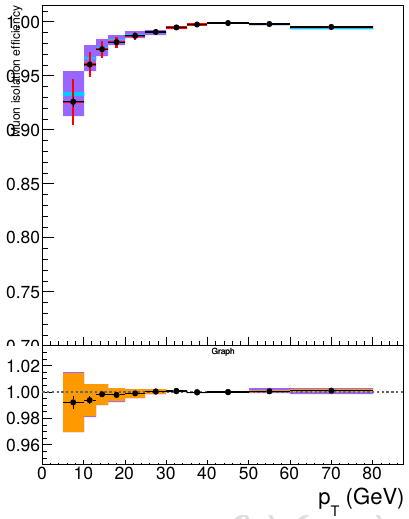
\includegraphics[scale=0.45]{ChapterAnalysis/figs/muon_iso_eff_endcap}}
	\legend{(a) muons in the barrel; (b) muons in the endcaps. In the upper panel the cyan (black) error bars show only the statistical uncertainty and the red (violet) ones represent the total uncertainty from MC (data). In the ratio plot the black error bars are for the statistical uncertainty, the orange ones for the systematical uncertainty and the violet ones for the total uncertainty.}
	\source{CMS COLLABORATION, 2016, p. 21.}
	\label{fig:muon_iso_efficiency}
\end{figure}

The efficiency to reconstruct a muon track in the inner detector is measured using tracks reconstructed only in the muon system. The method for measuring the tracking efficiency is the same as in \cite{bib:CMS-AN-15-215} and the results on 2016 data are briefly discussed here. The efficiency and data-to-simulation scale factors are measured from Z events as a function of $\eta$. The values of data-to-simulation scale factors used are from the ReReco version\footnote{That means a previous reconstructed version of the data collected by CMS have been reprocessed using new settings in the CMS simulation.} of the full dataset collected in 2016. The tracking efficiency in data and in simulation as a function of $\eta$ is shown in Fig.~\ref{fig:muon_tracking_efficiency}.

\begin{figure}[hbtp]{16cm}
	\caption{Tracking efficiency in data and simulation.}
	\centering
	\subfloat[]{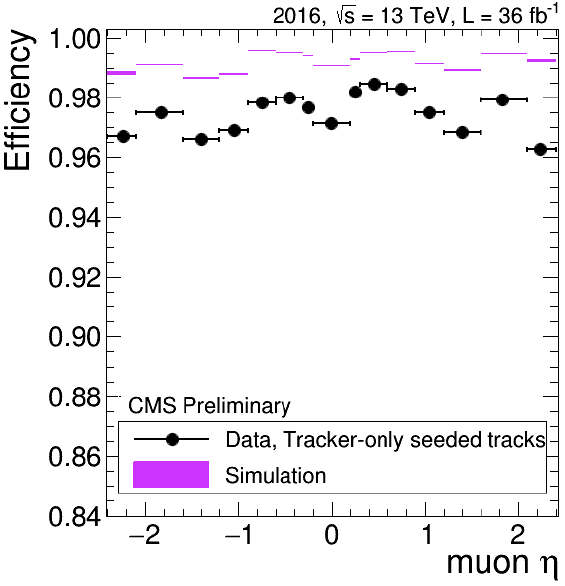
\includegraphics[scale=0.3]{ChapterAnalysis/figs/muon_tracking_eff_ptless10}}
	\quad
	\subfloat[]{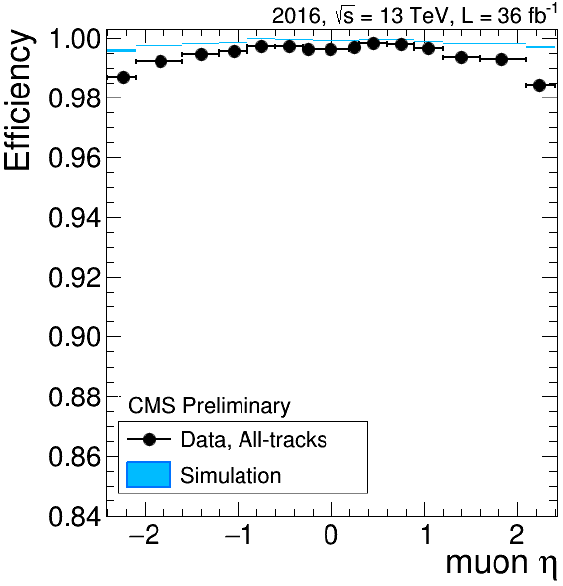
\includegraphics[scale=0.3]{ChapterAnalysis/figs/muon_tracking_eff_ptabove10}}
	\legend{(a) efficiency as a function of $\eta$ for muon $p_{T}<$ 10 GeV and (b) $p_{T}>$ 10 GeV.}
	\source{CMS COLLABORATION, 2016, p. 22.}
	\label{fig:muon_tracking_efficiency}
\end{figure}

The product of all data-to-simulation scale factors for muon tracking, reconstruction, identification, impact parameter and isolation requirements is used in the analysis.

\section{Photons and FSR Recovery}
The FSR recovery algorithm was considerably simplified with respect to what was done in RunI, while maintaining a similar performance. The selection of FSR photons is now only done per-lepton and no longer depends on any Z mass criteria, which significantly simplifies the building and selection of ZZ candidates. In the association of photons and leptons the rectangular cuts on $\Delta R(\gamma,l)$ and $E_{T,\gamma}$ have been replaced by a cut on $\Delta R(\gamma,l)/E_{T,\gamma}^{2}$.

Starting from the collection of photons provided by the PF algorithm (PF photons), the selection of photons and their association to a lepton proceeds as follows:
\begin{itemize}
	\item[1] The pre-selection of PF photons is done by requiring $p_{T}^{\gamma}>$ 2GeV, $|\eta^{\gamma}|<$ 2.4, and a RelPFiso$(\Delta R=0.3)<$ 1.8. The RelPFiso computation uses a threshold of 0.2GeV on charged hadrons, with a veto cone of 0.0001, and 0.5GeV on neutral hadrons and photons, with a veto cone of 0.01, also including the contribution from pileup vertices (with the same radius and threshold as per-charged isolation);
	\item[2] Supercluster veto: we remove all PF photons that match with any electron passing both the loose ID and SIP cuts. The matching is performed by directly associating the two PF candidates;
	\item[3] Photons are associated to the closest lepton in the event among all those that pass both the loose ID and SIP cuts;
	\item[4] Photons that do not satisfy $\Delta R(\gamma,l)/E_{T,\gamma}^{2}<$ 0.012 and $\Delta R(\gamma,l)<$ 0.5 are discarded;
	\item[5] If more than one photon is associated to the same lepton, we select the one with lowest $\Delta R(\gamma,l)/E_{T,\gamma}^{2}$;
	\item[6] Each selected FSR photon is removed from the isolation sum of all the leptons in the event that pass both the loose ID and SIP cuts. This concerns the photons that are in the isolation cone and outside the isolation veto of said leptons ($\Delta R<$ 0.4 AND $\Delta R>$ 0.01 for muons, and $\Delta R<$ 0.4 AND ($\eta^{SC}<$ 1.479 OR $\Delta R>$ 0.08) for electrons).
\end{itemize}

More details about the photon FSR optimization can be found in \cite{bib:CMS-AN-15-277,bib:CMS-AN-16-442}.


\section{Jets}
Jets are reconstructed through the anti-$k_{T}$ clustering algorithm using PF\footnote{Particle Flow: a set of algorithms developed by the CMS collaboration. It combine the signals coming from every CMS sub-detector in order to reconstruct the particle flow through CMS.} candidates after rejecting the charged hadrons that are associated to a pileup primary vertex. We use a distance parameter $R$ = 0.4. To reduce instrumental background, the loose working point for the jet identification suggested by the JetMET POG is applied. Jets are required to have $p_{T}>$ 30GeV and $|\eta|<$ 4.7 and are cleaned from any tight leptons and FSR photons by a separation criterion of $\Delta R(jet,l/\gamma)>$ 0.4. Since the calorimeter response to particles is not linear, Jet Energy Corrections (JEC) are needed to translate the measured jet energy to the true particle/parton energy. Standard JEC are applied on reconstructed jets, which consist of L1 Pileup, L2 Relative Jet Correction, L3 Absolute Jet Correction for both MC samples and data, and also residual calibration for data. For the purpose of reducing the background coming from $t\bar{t}$ events, the \textit{Combined Secondary Vertex} (CSV) algorithm is used as b-tagging algorithm. It combines information about the SIP, the secondary vertex (SV) and jet kinematics. These variables are combined through a likelihood ratio technique to compute the b-tag discriminator. In this analysis, a jet is considered to be b-tagged if the discriminator \textit{pfCombinedInclusiveSecondaryVertexV2BJetTags} $>$ 0.8484 (i.e. the jet passes the \textit{CSVv2M} "medium" working point). Data-to-simulation scale factors for b-tagging efficiency are provided for this working point for the full dataset as a function of jet $p_{T}$, $\eta$ and flavour. Such scale factors are applied to simulated jets by downgrading (upgrading) the b-tagging status of a fraction of the b-tagged (untagged) jets that have a scale factor smaller (larger) than one \cite{bib:CMS-AN-15-277,bib:CMS-AN-16-442}.

\section{Missing Transverse Energy}
The missing transverse energy (MET), $E_{p_{T}}^{miss}$, of an event
consists of the imbalance in the transverse plane with respect to the beam axis. Since the sum of momentum in the transverse plan must be zero, any imbalance is attributed to undetected particles (such as neutrinos) escaping the CMS detector. Raw $E_{T}^{miss}$ (PFMET) is defined as the magnitude of the negative vectorial sum of all reconstructed PF particles $p_{T}$,

\begin{equation}
\vec{E}_{T}^{miss} = - \sum_{j\epsilon all} \vec{p}_{T,i}
\end{equation}

An alternative definition of MET, which is called Type-I corrected $E_{p_{T}}^{miss}$, takes into account the JEC, correcting the MET for detector inefficiencies and non-linear responses in the calorimeters. The Type-I corrected MET is given by

\begin{equation}
\vec{E}_{T}^{miss} = - \left( \sum_{jets} \vec{p}_{T,jet}^{JEC} + \sum_{i \epsilon uncl.} \vec{p}_{T,i} \right)
\end{equation}

where the contribution of jets ($\vec{p}_{T,jet}^{JEC}$) and the remaining unclustered objects ($\vec{a}_{T,i}$) are accounted separately.

In order to improve signal-to-noise ratio several filters developed in the JETMET POG \cite{bib:CMS-AN-16-442} are used to select the events in this analysis. Such filters are presented in Tab.~\ref{tab:jetmet_filters}.

\begin{table}[hbtp]{16cm}
	\caption{Filters from JETMET POG used to improve signal-to-noise ratio.}
	\centering
	\begin{tabular}{p{6cm}|p{9cm}}
		\hline
		Filter & Description\\
		\hline
		HBHENoiseFilter \hspace{3cm} HBHENoiseIsoFilter & remove noisy events from the HCAL, where the HBHE scintillator produces anomalous signals with pulse shapes and pixel multiplicities discrepant from those from a clean signal\\
		\hline
		EcalDeadCellTriggerPrimitiveFilter & removes events with non-functioning ECAL data links, comparing the sum of energy deposited in each supercluster cell to the energy saturation of the trigger primitive\\
		\hline
		goodVertices & filter events with noisy vertex reconstruction (due to pileup effects) by requiring the reconstruction of at least one good vertex full filling the following criteria: high number of degree of freedom ($NPV>$ 4), collisions restricted along the z−axis ($zPV<$ 24cm) and small radius of the PV ($rPV<$ 2cm)\\
		\hline
		eeBadScFilter & removes events with noisy ECAL endcap superclusters\\
		\hline
		globalTightHalo2016Filter & removes events with enhanced MET from beam-halo particles which are in time with the beam\\
		\hline
		BadPFMuonFilter \hspace{3cm} BadChargedCandidateFilter & remove events with mis-reconstructed muon and charged hadron PF candidates\\
		\hline
	\end{tabular}
	\source{CMS COLLABORATION, 2016, p. 24. Adapted by the author.}
	\label{tab:jetmet_filters}
\end{table}


%%==========================================================================
\chapter{Event Selection}
\label{sec:event_selection}
%%==========================================================================
The selections performed in this analysis are designed to reconstruct a final state with four charged leptons ($4\mu$, $4e$ or $2e2\mu$) and MET. The four-lepton system must satisfy the SM Higgs selections described in \cite{bib:CMS-AN-16-442}. 

\section{Preselection}
The events must have fired at least one of the HLT paths presented in Chapter~\ref{sec:datasets}. They are also required to pass the MET filters described in Chapter~\ref{sec:physics_objects_selections}.

\section{Selection of the ZZ System}
The events with four lepton candidates are selected from what is called \textit{selected leptons}, which are the tight leptons defined in Chapter~\ref{sec:physics_objects_selections}. Such leptons have $SIP_{3D} <$ 4 as a vertex constraint and isolation cuts, where the FSR photons are removed from the isolation cone. A lepton cross cleaning, which discards leptons with $\Delta R \leq$ 0.05 from each other, is applied.

The building of a ZZ system from four candidate leptons proceeds according to the following sequential steps:
\begin{itemize}
	\item [1] \textbf{Z candidates}: are built from a pair of selected leptons of opposite charge and same flavor ($e^{+}e^{-}$, $\mu^{+}\mu^{-}$), having invariant mass satisfying $12 < m_{ll(\gamma)}<$ 120GeV, where the Z candidate mass takes into account (if any) a selected FSR photon;
	\item [2] \textbf{ZZ candidates}: are built from a pair of Z candidates which do not have common leptons (non-overlapping). The Z with closest $m_{ll(\gamma)}$ to the nominal Z boson mass is denoted as $Z_{1}$ and the second one is the $Z_{2}$. The built ZZ system must satisfy the following requirements:
	\begin{itemize}
		\item \textbf{Ghost removal}: any two leptons must have $\Delta R(\eta,\phi) > 0.02$;
		\item \textbf{Lepton $p_{T}$}: at least two out of the four leptons must have $p^{i}_{T} > 10$ and $p^{i}_{T} > 20$ GeV;
		\item \textbf{QCD suppression}: all opposite-sign lepton pair that can be built out of the four leptons (regardless of lepton flavor) must satisfy $m_{ll} > 4$ GeV. Here, the selected FSR photons are not included in the mass computation, since QCD-induced low mass dilepton (e.g. $J/\Psi$) may have photons nearby (e.g. from $\pi^{0}$);
		\item \textbf{$Z_{1}$ mass}: $m_{Z_{1}} > 40$ GeV;
		\item \textbf{Smart cut}: defining $Z_{a}$ and $Z_{b}$ as the mass-sorted alternative pairing Z candidate ($Z_{a}$ being the closest one to the nominal Z mass), require NOT($|m_{Z_{a}}-m_{Z}| < |m_{Z_{1}}-m_{Z}|$ AND $m_{Z_{b}} < 12$). Selected FSR photons are included in the $m_{Z}$'s computation. This cut discards 4$\mu$ and 4e candidates which have the alternative pairing similar to an on-shell Z + a low-mass pair $l^{+}l^{-}$;
		\item \textbf{Four-lepton invariant mass}: $m_{4l} > 70$ GeV;
		\item \textbf{Choice of the best ZZ candidate}: if more than one ZZ candidate survives the previous selections, the one with the highest four leptons $p_{T}$ scalar sum is chosen.
	\end{itemize}
	\item [3] \textbf{SM Higgs selection}: events containing at least one ZZ system satisfying all the previous selections are then used to tag the Higgs decaying into four lepton final state, as it is done for the SM Higgs analysis \cite{bib:CMS-AN-16-442};
	\item [4] \textbf{Signal region (SR)}: in order to enhance the presence of VBF events over the other SM Higgs production modes and the SM backgrounds, additional cuts are applied as discussed in the next section.
\end{itemize}

\section{VBF Signal Region (VBF-SR)}
\label{subsec:vbf_sr}
In order to optimize the analysis for the VBF production mode few additional requirements are imposed to the events selected after the steps described above (until step 3). These additional selections are:
\begin{itemize}
	\item \textbf{Number of jets}: events must have,
	\begin{itemize}
		\item EITHER, two or three jets from which at most one b-tagged jet;
		\item OR, more than three jets with no b-tagged jet;
	\end{itemize}
	\item \textbf{Four-lepton invariant mass}: events must have $118 \leq m_{4l} \leq 130$ GeV since the significant fraction of VBF yields is contained within that range. This $m_{4l}$ range is equal to the SM Higgs signal region adopted by CMS collaboration \cite{bib:JHEP11_047_2017}.
\end{itemize} 

Note that these VBF-SR requirements are similar to the standard ones used by CMS Collaboration defining the VBF category \cite{bib:JPhys-447-1-2013,bib:CMS-AN-16-442}. The difference, since the Artificial Neural Networks (ANNs) are the discriminants of interest in this analysis, is that the CMS MELA discriminant for VBF 2-jets category (denoted by $D_{qqH,2j}^{MELA}$ in the text) is not used to categorize events. The Tab.~\ref{tab:sm_higgs_yields} and Tab.~\ref{tab:vbf_sr_yields} show the yields for each process after the SM Higgs and VBF-SR selections, respectively. The Fig.~\ref{fig:control_plots} shows $m_{4l}$ distributions for such events. Note that those tables don't include yet the contribution coming from the reducible background (Z+X) that will be discussed in detail in Chapter~\ref{sec:zx_estimation}.

\begin{table}[hbtp]{16cm}
	\footnotesize
	\caption{Number of expected events for background and signal, with statistical uncertainty reported, and number of observed events after the SM Higgs selections.}
	\centering
	\begin{tabular}{c|c|c|c|c}
		\hline
		\rowcolor{light_gray}
		Process                     & 4$\mu$          & 4e              & 2e2$\mu$        & 4l\\
		ggH                         &  19.34$\pm$0.14 &  11.02$\pm$0.11 &  25.99$\pm$0.16 &   56.35$\pm$0.24\\
		VH                          &   1.45$\pm$0.01 &   0.92$\pm$0.01 &   2.14$\pm$0.01 &    4.51$\pm$0.01\\
		ttH                         &   0.36$\pm$0.00 &   0.23$\pm$0.00 &   0.48$\pm$0.00 &    1.07$\pm$0.01\\
		qqZZ+ZZJJ                   & 387.01$\pm$1.67 & 234.64$\pm$1.31 & 538.35$\pm$1.97 & 1160.00$\pm$2.90\\
		ggZZ                        &  65.81$\pm$0.09 &  43.85$\pm$0.08 & 102.32$\pm$0.13 &  211.98$\pm$0.18\\
		\hline
		$\sum$ backgrounds          & 473.97$\pm$1.68 & 290.66$\pm$1.31 & 669.29$\pm$1.98 & 1433.91$\pm$2.91\\
		\hline
		qqH (signal $m_{H}=125GeV$) &   1.86$\pm$0.01 &   1.10$\pm$0.01 &   2.53$\pm$0.01 &    5.49$\pm$0.02\\
		\hline
		Total expected              & 475.83$\pm$1.68 & 291.76$\pm$1.74 & 671.81$\pm$1.98 & 1433.91$\pm$2.92\\
		\hline
		Observed                    & 503             & 287             & 669             & 1459\\
		\hline
	\end{tabular}
	\source{The author, 2018.}	
	\label{tab:sm_higgs_yields}
\end{table}

\begin{table}[hbtp]{16cm}
	\footnotesize
	\caption{Number of expected events for background and signal and number of observed events after the VBF-SR selections.}
	\centering
	\begin{tabular}{c|c|c|c|c}
		\hline
		\rowcolor{light_gray}
		Process                     & 4$\mu$        & 4e            & 2e2$\mu$      & 4l\\
		ggH                         & 2.46$\pm$0.05 & 1.28$\pm$0.04 & 3.10$\pm$0.06 & 6.84$\pm$0.08\\
		VH                          & 0.34$\pm$0.00 & 0.20$\pm$0.00 & 0.46$\pm$0.00 & 1.00$\pm$0.01\\
		ttH                         & 0.05$\pm$0.00 & 0.03$\pm$0.00 & 0.06$\pm$0.00 & 0.14$\pm$0.00\\
		qqZZ+ZZJJ                   & 0.67$\pm$0.07 & 0.36$\pm$0.05 & 0.74$\pm$0.07 & 1.77$\pm$0.10\\
		ggZZ                        & 0.05$\pm$0.00 & 0.03$\pm$0.00 & 0.06$\pm$0.00 & 0.14$\pm$0.01\\
		\hline
		$\sum$ backgrounds          & 3.57$\pm$0.08 & 1.90$\pm$0.06 & 4.42$\pm$0.09 &  9.89$\pm$0.13\\
		\hline
		qqH (signal $m_{H}=125GeV$) & 1.05$\pm$0.01 & 0.58$\pm$0.01 & 1.39$\pm$0.01 &  3.02$\pm$0.02\\
		\hline
		Total expected              & 4.62$\pm$0.08 & 2.48$\pm$0.06 & 5.81$\pm$0.09 & 12.91$\pm$0.13\\
		\hline
		Observed                    & 5             & 2             & 10            & 17\\
		\hline
	\end{tabular}
	\source{The author, 2018.}	
	\label{tab:vbf_sr_yields}
\end{table}

\begin{figure}[hbtp]{16cm}
	\caption{Control plots of four-lepton invariant mass.}
	\centering
	\subfloat[]{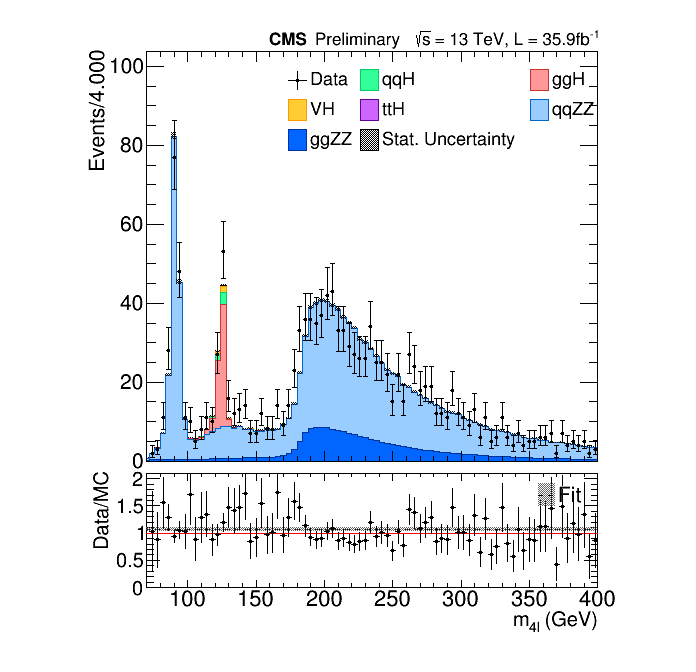
\includegraphics[scale=0.4,trim={2cm 0cm 2cm 0cm},clip]{ChapterAnalysis/figs/histo_mass4l_full_range}}
	\subfloat[]{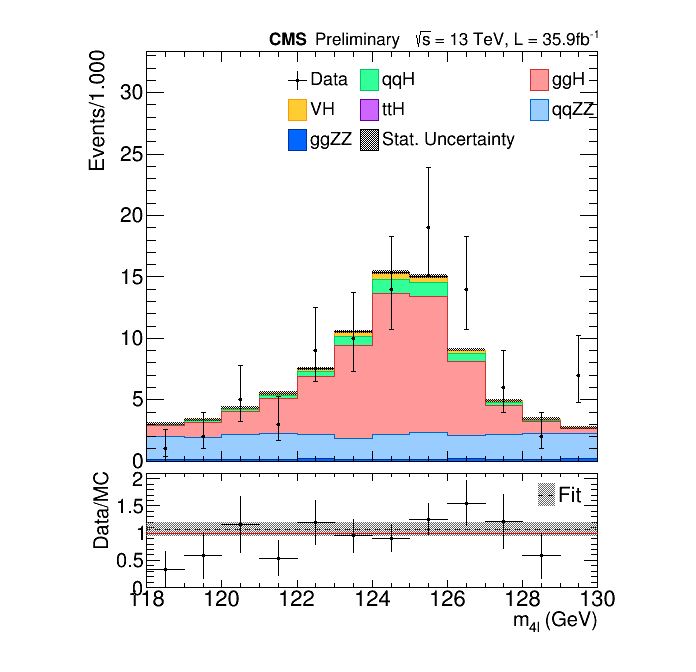
\includegraphics[scale=0.4,trim={2cm 0cm 2cm 0cm},clip]{ChapterAnalysis/figs/histo_mass4l_higgs_sr}}\\
	\subfloat[]{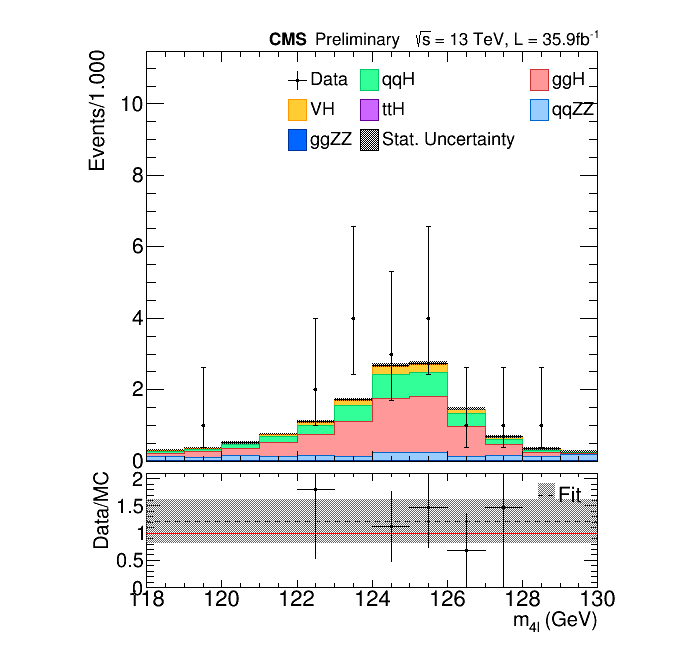
\includegraphics[scale=0.4,trim={2cm 0cm 2cm 0cm},clip]{ChapterAnalysis/figs/histo_mass4l_vbf_sr}}
	\legend{(a) events passing the SM Higgs selection; (b) events in the $m_{4l} = [118,130]$ GeV range; (c) events in the VBF signal region.}
	\source{The author, 2018.}	
	\label{fig:control_plots}		
\end{figure}


%%==========================================================================
\chapter{Neural Networks}
\label{sec:neural_networks}
%%==========================================================================
As shown on previous sections the Higgs VBF signal is quite small compared to its main background (the main Higgs production mode $ggH$). In order to enhance the signal efficiency this analysis was meant to be based on Artificial Neural Networks (ANNs) instead of applying rectangular cuts as usual. 

An ANN is an interconnected assembly of small processing units usually called neurons (also activations or nodes). Each of these units performs individual operations and communicates between themselves their results. Such a design was motivated by analogy with
the brain, which can be thought as a highly complex, nonlinear and parallel computer. It is estimated that the human brain has 100 billion neurons and each one of them typically receives thousands of connections from other neurons. The inter-neuron connections are mediated by electrochemical junctions, the so called synapses, which happens on branches of the cell called dendrites. These thousand of signals are then combined and depending of the result of this combination the neuron outputs a signal to its neighborhood \cite{bib:SimonHaykin,bib:KevinGurney}.

Similar to the brain, ANNs have the capability to learn from patterns and generalize the modeling of such patterns. This generalization means the possibility to correct identification of a pattern that was not seen before by the ANN during the learning process. The neurons contain a function which can receives also several arguments (inputs) and combine them into a single output value (Fig.~\ref{fig:nn_neuron_example}). There are several types of functions that can be used in the neurons and the choice of the best one might depend on each type of problem. The way the neurons are assembled also can be done in several ways, such that there are different architecture for the connections of the neurons. But a typical and well representative ANN architecture can be seen in Fig.~\ref{fig:neuron_and_dnn}. This kind of ANN is usually called Deep Neural Network (DNN) due to its many layers. Such ANN has shown capability to learn very complex tasks and its success comes from relatively recent improvements in the Machine Learning (ML) field \cite{bib:GlorotAndBendio2010,bib:NairAndHinton2010,bib:Zeiler_et_al2013}.

\begin{figure}[hbtp]{16cm}
	\caption{Illustration of an ANN neuron and a fully connected ANN.}
	\centering
	\subfloat[]{
		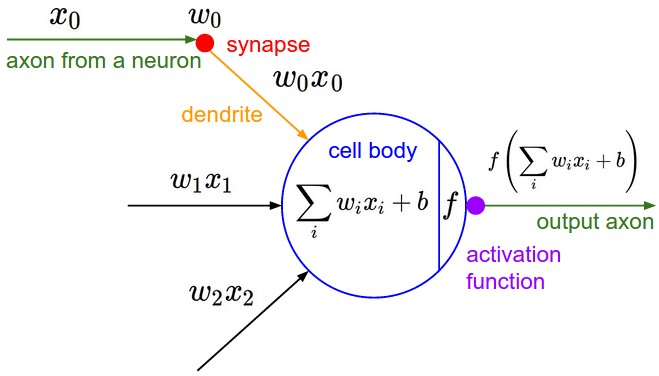
\includegraphics[width=0.56\textwidth]{ChapterAnalysis/figs/nn_neuron_example}
		\label{fig:nn_neuron_example}
	}
	\quad
	\quad
	\quad
	\subfloat[]{
		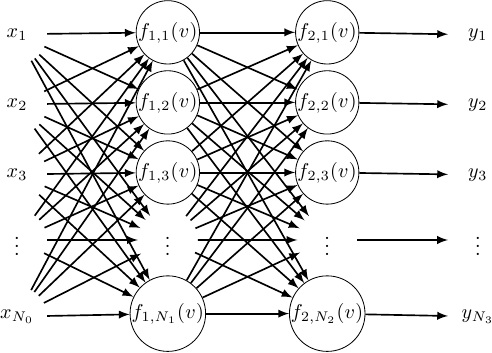
\includegraphics[width=0.62\textwidth]{ChapterAnalysis/figs/dnn_example}
		\label{fig:dnn_example}
	}
	\legend{(a) graphical representation of a neuron. Each input \textit{$x_i$} (from user or from the hidden neurons) is weighted by \textit{$w_i$} and summed to a bias \textit{b}. The sum is passed to a function (the activation function - neuron type) which outputs a vector of values (one for each input). (b) Graphical representation of a ANN with three hidden layers. In this type of ANN the outputs of all neurons from a previous layer are fed into the neurons of a next layer.}
	\source{JORDAN, 2018.}	
	\label{fig:neuron_and_dnn}
\end{figure}

Nowadays there are many different flavors of ANNs: Fully Connected Neural Networks (FC-NNs), Convolutional Neural Networks (CNNs), Long Short Term Memory Neural Networks (LSTM-NNs), etc \cite{bib:SimonHaykin}. In principle any of these types of ANNs can be used in any application but each one of them has some particular structure and workflow that benefits differently each application. In the present analysis the FC-NN was chosen. In a fully connected neural network the outputs from all the neurons in a previous layer are passed to all neurons in the next layer and this process happens across the entire ANN in a sequential way (Fig.~\ref{fig:dnn_example}).

\section{The Learning Process}
The way ANNs can be trained allows one to classify the learning process basically in two types: unsupervised and supervised. The former stands for the case when one doesn't know if a given dataset contains some pattern, in other words, if it is not possible to label the objects (read signal/background events) in the dataset. The ANN can be still trained to find out possible patterns existing in the dataset. The supervised procedure is the opposite situation in which one knows that the dataset contains patterns and such patterns are known. The ANN is then trained to correctly assign a given label to a given example. The labels can arbitrarily be chosen and usually for classification task of two classes one uses 0 or 1 for labeling the examples. In order to verify the performance of labels assignment there is a function, usually called \textit{loss} (or cost/risk), which measures the error between the ANN response and what is expected \cite{bib:SimonHaykin}. The output of the \textit{loss} function is the main input used to modify the ANN parameters in order to evolve the modeling of the data. The modification in the ANN parameters (Fig.~\ref{fig:nn_neuron_example}) is done by an algorithm called \textit{back-propagation} which consists basically of an application of the chain rule for partial derivatives.

Exemplifying such process, let's assume a neuron $j$ in a intermediate layer of a neural network. Calling $w_{ji}$ as the weight assigned by that neuron $j$ to an input $y_{i}(n)$ at a given iteration $n$, then such neuron produces a \textit{local field} given by

\begin{equation}
v_{j}(n) = \sum_{i=1}^{m} w_{ji}(n)y_{i}(n) + b_{j}(n)
\label{neuron_local_field}
\end{equation}

in which $m$ stands for the total number of inputs received by the neuron and $b_{j}(n)$ is the so called bias (which is just one value per neuron). This \textit{local field} is then given as an argument to an activation function (represented by $\mathit{f}$ in Fig.~\ref{fig:neuron_and_dnn}) which produces the \textit{signal function} $y_{j}(n)$ of the neuron $j$ at iteration $n$,

\begin{equation}
y_{j}(n) = \mathit{f}[v_{j}(n)]
\end{equation}

It is possible to compute an instantaneous error for the neuron $j$ (Eq.~\ref{eq:instant_error}) using its \textit{signal error} $e_{j}(n)$ which is defined as the difference between the neuron \textit{signal function} $y_{j}(n)$ (its output after the activation function) and the expected \textit{response} $d_{j}(n)$. Note that, the expected response $d_{j}(n)$ can be the label identifying a training example - for neurons in the output layer - or an actual response that a hidden neuron - in the intermediate layers - should have based on the example label. The Eq.~\ref{eq:instant_error} is the core of the so called \textit{loss} or \textit{empirical risk} and it is an example of \textit{loss} function used here in order to exemplify the ANN learning process but, be aware that there are other types. Summarizing, the processes described so far can be graphically represented as shown in Fig.~\ref{fig:neuronj_signal_flow}.

\begin{equation}
\label{eq:instant_error}
\mathcal{E}(n) = \frac{1}{2} e_{j}^{2}(n), ~~\mathrm{with}~~ e_{j}(n) = d_{j}(n) - y_{j}(n)
\end{equation}

\begin{figure}[hbtp]{16cm}
	\caption{The flow of signal through the neuron $j$ up to its instantaneous error $e_{j}$.}
	\centering
	\includegraphics[scale=0.5]{ChapterAnalysis/figs/neuronj_signal_flow}
	\source{HAYKIN, 2009, p. 129. Adapted by the author.}
	\label{fig:neuronj_signal_flow}
\end{figure}

Now, taking the partial derivative of the \textit{loss} by application of the chain rule one gets,

\begin{equation}
\frac{\partial \mathcal{E}(n)}{\partial w_{ji}} = \frac{\partial \mathcal{E}(n)}{\partial e_{j}(n)} ~ \frac{\partial e_{j}(n)}{\partial y_{j}(n)} ~ \frac{\partial y_{j}(n)}{\partial v_{j}(n)} ~ \frac{\partial v_{j}(n)}{\partial w_{ji}(n)}.
\end{equation}

and replacing the derivatives accordingly like so,

\begin{equation}
\frac{\partial \mathcal{E}(n)}{\partial e_{j}(n)} = e_{j}(n)
\end{equation}

\begin{equation}
\label{eq:signal_error_partial}
\frac{\partial e_{j}(n)}{\partial y_{j}(n)} = -1
\end{equation}

\begin{equation}
\frac{\partial y_{j}(n)}{\partial v_{j}(n)} = \mathit{f}'[v_{j}(n)]
\end{equation}

\begin{equation}
\frac{\partial v_{j}(n)}{\partial w_{ji}(n)} = y_{i}(n)
\end{equation}

one reaches to

\begin{equation}
\label{eq:loss_partial}
\frac{\partial \mathcal{E}(n)}{\partial w_{ji}} = -e_{j}(n) ~ \mathit{f}'[v_{j}(n)] ~ y_{i}(n).
\end{equation}

Finally, the correction applied to the weights $w_{ji}$ is given by the \textit{delta rule} as

\begin{equation}
\label{eq:error_correction}
\Delta w_{ji}(n) = - \eta \frac{\partial \mathcal{E}(n)}{\partial w_{ji}}
\end{equation}

where the signal "-" accounts for the descending gradient in the weights space (that is, it seeks for a direction in which the weight change leads to decreasing of $\mathcal{E}(n)$). The $\eta$ term is the so called \textit{learning rate} of the back-propagation algorithm. The Eq.~\ref{eq:error_correction} is the core of the synaptics ($w_{ji}$) update within the neural network. Replacing the Eq.~\ref{eq:loss_partial} into Eq.~\ref{eq:error_correction} yields

\begin{equation}
\label{eq:error_correction_simplified}
\Delta w_{ji}(n) = \eta ~ \delta_{j}(n) ~ y_{i}(n), ~~\mathrm{with}~~\delta_{j}(n) = \frac{\partial \mathcal{E}(n)}{\partial v_{j}(n)}
\end{equation}

The term $\delta_{j}(n)$ is the \textit{local gradient}. From this point there are two situations now:
\begin{itemize}
\item [1] When the neuron is located in the output layer: in such case that neuron is supplied by the labels classifying the examples (which is its \textit{expected response} $v_{j}$) and thus, by Eq.~\ref{eq:instant_error}, one has the error and can compute the \textit{local gradient} $\delta_{j}(n)$;
\item [2] When the neuron is in a hidden layer some complications arise but still Eq.~\ref{eq:error_correction} holds. The Fig.~\ref{fig:hidden_neuronj_signal_flow} showns a scheme of the signal flow in this case. According to Eq.~\ref{eq:error_correction_simplified} and Eq.~\ref{eq:signal_error_partial} it is possible to redefine the \textit{local gradient} for a hidden neuron $j$ as

\end{itemize}
\begin{figure}[hbtp]{16cm}
	\caption{The flow of signal through a hidden neuron $j$ up to its \textit{signal function} $y_{j}(n)$ which is forwarded as an input to an neuron $k$ in an output layer. Note that, the \textit{activation function} can now be different between the layers and they are represented as $f_{j}$ and $f_{k}$ for the neurons $j$ and $k$, respectively.}
	\centering
	\includegraphics[scale=0.4]{ChapterAnalysis/figs/hidden_neuronj_signal_flow}
	\source{HAYKIN, 2009, p. 132. Adapted by the author.}	
	\label{fig:hidden_neuronj_signal_flow}
\end{figure}

\begin{equation}
\label{eq:local_gradient_hidden}
\delta_{j}(n) = - \frac{\partial \mathcal{E}(n)}{\partial y_{j}(n)} ~ \frac{\partial y_{j}(n)}{\partial v_{j}(n)} = - \frac{\partial \mathcal{E}(n)}{\partial y_{j}(n)} ~ \mathit{f}'[v_{j}(n)].
\end{equation}

From Eq.~\ref{eq:instant_error} and Fig.~\ref{fig:hidden_neuronj_signal_flow} it is clear that $\mathcal{E}(n) = (1/2) \sum_{(k~\epsilon~C)} e_{k}^{2}(n)$. Differentiating this expression with respect to $y_{j}(n)$ one has

\begin{equation}
\label{eq:loss_partial_hidden_neuron}
\frac{\partial \mathcal{E}(n)}{\partial y_{j}(n)} = \sum_{k~\epsilon~C} e_{k}(n) ~ \frac{\partial e_{k}(n)}{\partial y_{j}(n)} \equiv \sum_{k~\epsilon~C} e_{k}(n) ~ \frac{\partial e_{k}(n)}{\partial v_{k}(n)} ~ \frac{\partial v_{k}(n)}{\partial y_{j}(n)}
\end{equation}

Now, from Fig.~\ref{fig:hidden_neuronj_signal_flow} and the previous discussions one sees that,

\begin{eqnarray}
e_{k}(n) &=& d_{k}(n) - y_{k}(n) \equiv d_{k}(n) - \mathit{f}_{k}'[v_{k}(n)] \\
\label{eq:ek_partial}
\frac{\partial e_{k}(n)}{\partial v_{k}(n)} &=& -\mathit{f}_{k}'[v_{k}(n)]\\
v_{k}(n) &=& \sum_{j=1}^{m} w_{kj}(n) y_{j}(n) + b_{k}(n)\\
\label{eq:vk_partial}
\frac{\partial v_{k}(n)}{\partial y_{i}(n)} &=& w_{kj}(n)
\end{eqnarray}

and, using Eq(s).~\ref{eq:ek_partial} and \ref{eq:vk_partial} into \ref{eq:loss_partial_hidden_neuron} one has

\begin{eqnarray}
\label{eq:dedj_hidden}
\nonumber
\frac{\partial \mathcal{E}(n)}{\partial y_{j}(n)} &=& - \sum_{k~\epsilon~C} e_{k}(n) ~ \mathit{f}_{k}'[v_{k}(n)] ~ w_{kj}(n)\\
                                                  &=& - \sum_{k~\epsilon~C} \delta_{k}(n) ~ w_{kj}(n)
\end{eqnarray}

where the definition of \textit{local gradient} has been used. Finally, using Eq.~\ref{eq:dedj_hidden} in \ref{eq:local_gradient_hidden} one finds that the \textit{back-propagation} formula for the hidden neuron $j$ is

\begin{equation}
\label{eq:local_gradient_hidden_final}
\delta_{j}(n) = \mathit{f}_{j}'[v_{j}(n)] ~ \sum_{k~\epsilon~C} \delta_{k}(n) ~ w_{kj},~~\mathrm{neuron}~j~\mathrm{is~hidden}.
\end{equation}

Note that, the sum in Eq.~\ref{eq:local_gradient_hidden_final} is over all the neurons in the output layer. Also note that, $e_{k}(n)$ can be extended to internal layers, such that, it will correspond to the signal errors coming from neurons in the forward hidden layers.


\section{Developing and Training the Neural Networks}
\label{sec:developing_training_neural_networks}
In this analysis the base software used to build up and train the ANNs
is Keras \cite{bib:KerasWebPage}. Keras is a widely used and powerful set of python libraries that allows one to quickly create any type of known ANN. It contains sets of modules that simplify much of the coding needed by the user. Keras has recently been integrated into TMVA \cite{bib:JPhysConfSer_898_072046_2017} and the user has the flexibility to either prepare a C++ code version or to transfer a python version to TMVA which plugs it into Keras. Note however that in the beginning of this analysis that wasn't available and an entire Keras-python framework was developed to make the studies. Using recent version of TMVA cross-checks were made comparing the results got by Keras-python and Keras-TMVA, and the results are in agreement.

\section{Preparation of the Datasets}
\label{subsec:datasets_preparation}
The Neural Networks have been trained using the simulated samples described in Chapter~\ref{sec:datasets} and only with the events passing the selections defining the VBF-SR. As it will be discussed later the variables used into the final ANNs are the leptons and jets three-momentum (that is, $p_{T}$, $\eta$ and $\phi$). The distribution of such variables, for both MC and Data, is shown in Fig.~\ref{fig:ann_input_variables} as a cross-check of the variables shape and Data-MC agreement (the low binning has been chosen due to the low statistic available for Data at the VBF-SR). The Z+X background on those pictures is derived via a stablished CMS data-driven method, which is described in Chapter~\ref{sec:zx_estimation}.

\begin{figure}[hbtp]{16cm}
	\caption{Monte Carlo and Data distribution of the variables used as inputs to train the ANNs in this analysis (continue).}
	\centering
	\subfloat[]{
		\includegraphics[scale=0.23,trim={2cm 1cm 2cm 1cm},clip]{ChapterAnalysis/figs/vbf_l1_pt}
	}
	\subfloat[]{
		\includegraphics[scale=0.23,trim={2cm 1cm 2cm 1cm},clip]{ChapterAnalysis/figs/vbf_l1_eta}
	}
	\subfloat[]{
		\includegraphics[scale=0.23,trim={2cm 1cm 2cm 1cm},clip]{ChapterAnalysis/figs/vbf_l1_phi}
	}\\
	\subfloat[]{
		\includegraphics[scale=0.23,trim={2cm 1cm 2cm 1cm},clip]{ChapterAnalysis/figs/vbf_l2_pt}
	}
	\subfloat[]{
		\includegraphics[scale=0.23,trim={2cm 1cm 2cm 1cm},clip]{ChapterAnalysis/figs/vbf_l2_eta}
	}
	\subfloat[]{
		\includegraphics[scale=0.23,trim={2cm 1cm 2cm 1cm},clip]{ChapterAnalysis/figs/vbf_l2_phi}
	}\\
	\subfloat[]{
		\includegraphics[scale=0.23,trim={2cm 1cm 2cm 1cm},clip]{ChapterAnalysis/figs/vbf_l3_pt}
	}
	\subfloat[]{
		\includegraphics[scale=0.23,trim={2cm 1cm 2cm 1cm},clip]{ChapterAnalysis/figs/vbf_l3_eta}
	}
	\subfloat[]{
		\includegraphics[scale=0.23,trim={2cm 1cm 2cm 1cm},clip]{ChapterAnalysis/figs/vbf_l3_phi}
	}\\
	\subfloat[]{
		\includegraphics[scale=0.23,trim={2cm 1cm 2cm 1cm},clip]{ChapterAnalysis/figs/vbf_l4_pt}
	}
	\subfloat[]{
		\includegraphics[scale=0.23,trim={2cm 1cm 2cm 1cm},clip]{ChapterAnalysis/figs/vbf_l4_eta}
	}
	\subfloat[]{
		\includegraphics[scale=0.23,trim={2cm 1cm 2cm 1cm},clip]{ChapterAnalysis/figs/vbf_l4_phi}
	}
\end{figure}
\begin{figure}[hbtp]{16cm}
	\setcounter{figure}{30}
	\ContinuedFloat
	\caption{Monte Carlo and Data distribution of the variables used as inputs to train the ANNs in this analysis (conclusion).}
	\centering
	\subfloat[]{
		\includegraphics[scale=0.23,trim={2cm 1cm 2cm 1cm},clip]{ChapterAnalysis/figs/vbf_j1_pt}
	}
	\subfloat[]{
		\includegraphics[scale=0.23,trim={2cm 1cm 2cm 1cm},clip]{ChapterAnalysis/figs/vbf_j1_eta}
	}
	\subfloat[]{
		\includegraphics[scale=0.23,trim={2cm 1cm 2cm 1cm},clip]{ChapterAnalysis/figs/vbf_j1_phi}
	}\\
	\subfloat[]{
		\includegraphics[scale=0.23,trim={2cm 1cm 2cm 1cm},clip]{ChapterAnalysis/figs/vbf_j2_pt}
	}
	\subfloat[]{
		\includegraphics[scale=0.23,trim={2cm 1cm 2cm 1cm},clip]{ChapterAnalysis/figs/vbf_j2_eta}
	}
	\subfloat[]{
		\includegraphics[scale=0.23,trim={2cm 1cm 2cm 1cm},clip]{ChapterAnalysis/figs/vbf_j2_phi}
	}\\
	\subfloat[]{
		\includegraphics[scale=0.23,trim={2cm 1cm 2cm 1cm},clip]{ChapterAnalysis/figs/vbf_j3_pt}
	}
	\subfloat[]{
		\includegraphics[scale=0.23,trim={2cm 1cm 2cm 1cm},clip]{ChapterAnalysis/figs/vbf_j3_eta}
	}
	\subfloat[]{
		\includegraphics[scale=0.23,trim={2cm 1cm 2cm 1cm},clip]{ChapterAnalysis/figs/vbf_j3_phi}
	}
	\legend{First lepton (a) $p_{T}$, (b) $\eta$ and (c) $\phi$; second lepton (d) $p_{T}$, (e) $\eta$ and (f) $\phi$; third lepton (g) $p_{T}$, (h) $\eta$ and (i) $\phi$; forth lepton (j) $p_{T}$, (k) $\eta$ and (l) $\phi$; first jet (m) $p_{T}$, (n) $\eta$ and (o) $\phi$; second jet (p) $p_{T}$, (q) $\eta$ and (r) $\phi$;  third jet (s) $p_{T}$, (t) $\eta$ and (u) $\phi$.}
	\source{The author, 2018.}
	\label{fig:ann_input_variables}
\end{figure}


In order to optimize the analysis and properly handle the usage of the third jet in the events, two jet-based categories have been defined and are labeled as \textbf{Njet2} and \textbf{Njet3} from now on. The \textbf{Njet2} category comprehend the events with exactly two jets while the \textbf{Njet3} category are composed by the events with at least three jets. For each of this category a ANN was developed.

Assuring an adequate distribution of the events when splitting them, forming the exclusive training and testing sets, the following procedure was adopted for the VBF-SR events in each jet-based category:
\begin{itemize}
	\item[1] Each simulated process has three samples one for each final state ($4\mu$, $4e$ and $2e2\mu$). Those three samples were merged into just a single sample with the events from each final state being randomized, such that the final states randomly populated the merged sample;
	\item[2] The merged and randomized samples for each process were divided into two parts: one containing $80\%$ of the total events and one containing the remaining $20\%$;
	\item[3] The first and second parts from each process were merged and once more the events were randomized in order to randomly populate each process inside the two parts;
\end{itemize}

The merged first parts constitutes the training set, that is the set of events used to train the ANN. The merged second parts constitute the testing set which is used to test the trained ANNs. Note that the two sets are completely independent such that the ANN was tested with completely new (and thus unseen by the ANN) events. As explained in Chapter~\ref{sec:neural_networks} the ANN training is very similar to a fit procedure and thus few examples (points) produces fits with large errors.

\section{Scaling Events Contribution in the Training}
\label{subsec:scale_train}
In the beginning of this analysis the ANN trainings were carried out without taking into account any kind of event weight. In such way all events are seen by the ANN in an equal basis. Keras has some features that allows one to include scale factor (a weight for each example event) which are in general used to balance the training when the number of events from different classes are very different. In the physics scenario one could use the individual MC event weights ($\sigma.\epsilon.BR$) or yet the sum of those weights (which constitutes the expected yields). The advantage of the first approach is that some events, from signal or background, crossing the classes zones defined by the ANN could have small weights and would be worthy to allow them to come in with the benefit to possibly improve  the final discrimination. The disadvantage is that the individual weights might not keep the hierarchical contribution of each process since the expected cross-section is divided by the number of events (such that if one have a large number of events the weights might become smaller for important processes than the ones for other small processes).

Both approaches were tested. The weight is used by Keras as a scale factor for the \textit{loss} function such that during the training each example is seen by the ANN with a different importance. That affects the direction in which the \textit{minimizer} computes the gradients of the \textit{loss} function. The advantage of doing so is that even if a process has few events, which is very frequent in many analysis, it will be properly taken into account with respect to the other process having more events. The Fig.~\ref{fig:scaling_training_effect} shows the impact of scaling the \textit{loss}. In the beginning of the analysis the sample ggH-minlo was produced slightly different from the other samples: the leptons were sorted by $p_{T}$ in the $4\mu$ final state. Without weighting the events during the training the typical ROC curves\footnote{ROC stands for Receive and Operative Curve which is a figure of merit commonly used in fields like medicine and shows a discriminant efficiency for filtering out signal versus background.} observed were like the one showed in Fig.~\ref{fig:nn_no_scale_roc}. Once the weights were introduced the discrimination of VBF and ggH processes increased significantly as showed in Fig.~\ref{fig:nn_scale_roc}. Although this is not a physical property and thus had to be fixed, this shown the big importance of scaling the events contribution. It shows that the ANN may not learn some features from a process if a scaling is not applied. As seen in Tab.~\ref{tab:vbf_sr_yields} ggH has the biggest yield and has a relatively good number of events but still without weighting it the small difference was not taken into account by the ANN. Since there all the further developed studies were done with the events weighted.

\begin{figure}[hbtp]{16cm}
	\caption{ROC curves comparing the performance of a trained ANN, the VBF MELA discriminant and $D_{jet}$.}
	\centering
	\subfloat[]{
		\includegraphics[width=0.35\textwidth]{ChapterAnalysis/figs/3jets_pt_eta_phi_no_weight_vbf_vs_all_leptons_sorting_issue}
		\label{fig:nn_no_scale_roc}
	}
	\quad
	\quad
	\subfloat[]{
		\includegraphics[width=0.35\textwidth]{ChapterAnalysis/figs/3jets_pt_eta_phi_weight_sum_vbf_vs_all_leptons_sorting_issue}
		\label{fig:nn_scale_roc}
	}
	\legend{(a) the performance of ANN without scaling the \textit{loss}; (b) performance after scaling the \textit{loss}.}
	\source{The author, 2018.}
	\label{fig:scaling_training_effect}
\end{figure}

\section{The Training Procedure}
\label{subsec:training_procedure}
Training MVA methods is a procedure that always need to be done in multiple fronts. It is hard to guarantee that for a set of inputs a set of MVA training parameters are the optimal choice, since there is an infinity of combinations that one can build. Those configurations (including the training dataset) can strongly affect the evolution of the MVA training. 

In the same time one needs to be careful when doing the training since crucial issues can occur and lead to a very bad MVA model. An ANN training commonly leads (or present them while on going) to one of three main situations: 
\begin{itemize}
\item \textbf{underfit}: occurs when an ANN has too few parameters (the $w_i$'s and $b_i$'s), making it not capable to model the training data. This behavior can be identified by looking the ANN loss curve not decreasing. Such issue can be, tentatively, solved by increasing the number of parameters (that is, using more neurons) and the training time. Notice though that the ANN will always reach some level where it can not learn more features from the training data, that is the ANN learning limit;
\item \textbf{goodfit}: this is the ideal situation. The ANN has a sufficient number of parameters and have been enough trained such that it properly models the training data and become able to make correct predictions on unseen data (that means the ANN is well generalized);
\item \textbf{overfit}: occurs when an ANN has too many parameters or is trained too much. In this situation the ANN starts to model the noise on the training data, that is, its variance (which is pretty common to happen in measured quantities). This usually makes the ANN very good in the modeling of the training data but it becomes very bad on making predictions for unseen data. This can be noticed by looking the training and the validation/testing loss diverging from each other and, usually the validation loss reaches a minimum and then starts to increase again. The best solution for this issue is the increasing of the training data set, which is not always possible. So, the other two tentative procedures are the reduction of the number of parameters and the reduction of the training time.
\end{itemize}

A good example of these three cases is show in Fig.~\ref{fig:training_issues}, which represents the situation of using an ANN to model a set of data distributed like sine/cosine shape. In Fig.~\ref{fig:training_issues}(a) the ANN had too few parameters and thus can't model the data distribution, while in (b) is has enough parameters such it can describe with good agreement the data. Fig.~\ref{fig:training_issues}(c) shows the extreme case when the ANN has too many parameters and thus has too many degrees of freedom to fit all data points. Since the loss is computed based on the difference between the ANN prediction and the original data, it goes very close to zero and one could think the ANN is perfect. However, as one let more data appear (which would be around the sine/cosine shape) it will see the ANN can't correctly predict such unseen data. Remember that on CMS collected data one does not know which physics process produced each event and thus is very important to have an ANN that can make right predictions on unseen Monte Carlo events.

\begin{figure}[hbtp]{16cm}
	\caption{Example of the three main situations that can occur during an ANN training.}
	\centering
	\subfloat[]{\includegraphics[scale=0.8]{Slides/figs/underfit}}
	\quad
	\subfloat[]{\includegraphics[scale=0.8]{Slides/figs/goodfit}}
	\quad
	\subfloat[]{\includegraphics[scale=0.8]{Slides/figs/overfit}}
	\legend{(a) the underfit; (b) the goodfit; (c) the overfit.}
	\source{JORDAN, 2018.}
	\label{fig:training_issues}
\end{figure}

The underfit, goodfit and overfit can also be seen by looking the training and the validation/testing losses. This is a good thing when one can not compare the expectations to the ANN predictions as shown in Fig.~\ref{fig:training_issues}. A common recommendation found in the literature \cite{bib:SimonHaykin,bib:KevinGurney,bib:GlorotAndBendio2010,bib:NairAndHinton2010,bib:Zeiler_et_al2013,bib:glouppe-ESWB-2018-1} is represented in Fig.~\ref{fig:learning_curves} which shows the loss variation during an ANN training. The loss is the what is called "error" in the figure. As one can see the underfit and the overfit are two extremes situations in which the ANN are not good. It can either poorly model the data or poorly make reasonable predictions. The ideal point where to stop an ANN training is when the validation loss starts to increase and diverges from the training loss behavior.

\begin{figure}[hbtp]{16cm}
	\caption{The underfit, goofit and overfit seen from the training and validation/testing loss curves.}
	\centering
	\includegraphics[scale=0.8,trim={2cm 0cm 0cm 2cm},clip]{Slides/figs/early_stop}
	\source{JORDAN, 2018.}
	\label{fig:learning_curves}
\end{figure}

In order to optimize the studies with the ANN in this analysis a framework was developed in python. It has the feature to build up through Keras different ANN architectures and perform multiple parallel scans. These scans can run over different sets of inputs and the several parameters that needs to be configured for the training. The result of each ANN training can be retrieved to produce plots which are used to validate and classify the quality of each training (one can check if over-fitting happened, for instance). 

The set of tested inputs includes combinations of the leptons and jets kinematic variables ($p_{T}$, $\eta$, $\phi$ and $E$), MET, Njets and Nbjets. The scanned ANN parameters are summarized in the Tab.~\ref{tab:training_parameters_summary}. These parameters are:
\begin{itemize}
	\item \textbf{Pre-processing}: it is a usual practice in Machine Learning field to apply some operation in the ANN inputs in order to standardize them (keep them in the same range of values for instance). In the scans done the pre-processing showed negligible effects and it was decided to not adopt such procedure for further studies. Note that, when pre-processing is applied in the training it will be need to also apply the same procedure when using the trained ANN (otherwise the results will be mistaken, since the ANN are expecting preprocessed inputs). One also should note that preprocessing changes the input variables what may destroy the possibility of the ANN reconstruct some important property(e.g. invariant masses);
	\item \textbf{Topology}: the architecture of the ANN, that is, the number of hidden layers, neurons and the neuron type. In Keras there are several types of neuron which even includes possible learning parameters (during training). The \textit{Rectified Linear Unity} (ReLU) is the most recommended due to its property of non-vanishing gradient;
	\item \textbf{Batch size}: the number of events in a subset from the training set used to compute the gradients and update the \textbf{$w_{i}$}'s and \textbf{$b$} in each neuron;
	\item \textbf{Epochs}: the number of iterations over the full training set. The total number of iterations is a combination of the size of the training set, the batch size and the number of epochs. For instance, setting a training of 10 epochs and a batch size of 10 for a training set size of 100 means that Keras performs $10^{2}$ updates on the \textbf{$w_{i}$}'s and \textbf{$b$}'s;
	\item \textbf{Early stop}: a parameter to set the number of epochs which Keras should wait if not improvement in the loss function is observed. If still not improvement is seen after that number of epochs the training is stopped;
	\item \textbf{Minimizer}: is the method to compute the gradients. There are several options in Keras (SGD, Adam, RMSprop, etc.) and after testing most of them it was decided to keep Adam. Adam stands for Adaptive Momentum and has the property of fast convergence due to a ANN updating directed towards the loss function minimum. This minimizer is widely applied in ML studies;
	\item \textbf{Scaling}: Keras allows one to scale the loss function by some weight that can be independent for each training example or the same for a entire class (signal or background, for instance). It was tested the impact of using the expected yield (cross section) of each process and the individual weights of each event ($\sigma.\epsilon.BR$);
	\item \textbf{Dropout}: it is a procedure in which keras randomly sets a fraction of the input units (literally the ANN input variables or then neurons outputs - which are inputs for forward neurons in the net) to zero at each update during the ANN training. This mechanism helps to prevent the over-fitting issue and also can build up more complex models. Keras allows one to apply this procedure in each layer independently (so one can apply it just on the first layer and not in the other ones);
\end{itemize}

\begin{table}[hbtp]{16cm}
	\centering
	\caption{Summary of the scanned parameters during ANN trainings.}
	\begin{tabular}{c|l}
		\hline
		\rowcolor{light_gray}
		Parameter      & Tested options\\
		\hline
		Inputs         & leptons/jets($p_{T}$,$\eta$,$\phi$), MET\\
		\hline
		Pre-processing & none, normalization, standardization\\
		\hline
		Topologies     & 7:5:3, 9:7:5, 11:9:7, 15:10:5, 21:13:8, 10:10:10:10,\\
		               & 30, 100, 100:100:50, 1000\\
		\hline
		Early stop     & 100, 600, 3000\\
		\hline
		Minimizer      & SGD, Adam, Adagrad, Adadelta, RMSprop\\
		\hline
		Batch size     & 1, 5, 32, 64, 128, 786\\
		\hline
		Neuron         & ReLU, SeLU\\
		\hline
		Loss Scaling   & cross section, $\sigma.\epsilon.BR$ (event weight)\\
		\hline
		Dropout        & none, 0.1, 0.3, 0.5, 0.7, 0.9, 0.99, 0.3:0.4:0.2, 0.5:0.25:0.1\\
		\hline
	\end{tabular}
	\source{The author, 2018.}	
	\label{tab:training_parameters_summary}	
\end{table}

The ANNs achieved through these trainings are produced together with some plots which are used to validate the choice of the best ANN architecture. These plots comprehend the metrics adopted (ROCs, $\epsilon_{s}.\pi$, $\sigma$) and the ANN distributions for the training and test sets, which helps to check if there was over-fitting for a given configuration. Fig.~\ref{fig:nn_training_outputs} shows these plots. The ROCs curve from training and test sets are also used to check if there was over-fitting. The plots in Fig.~\ref{fig:nn_training_outputs} show a example in which the ANN is considered good.

\begin{figure}[hbtp]{16cm}
	\caption{Example of checking plots produced during ANNs training.}
	\centering		
	\subfloat[]{
		\includegraphics[scale=0.35]{ChapterAnalysis/figs/MELAOvertrainingCheck_example}
		\label{}
	}
	\subfloat[]{
		\includegraphics[scale=0.35]{ChapterAnalysis/figs/NNOvertrainingCheck_example}
		\label{}
	}\\		
	\subfloat[]{
		\includegraphics[scale=0.34]{ChapterAnalysis/figs/ComparisonMCsEffPurity_example}
		\label{}
	}
	\subfloat[]{
		\includegraphics[scale=0.34]{ChapterAnalysis/figs/ComparisonMCsSignificance_example}
		\label{}
	}\\
	\subfloat[]{
		\includegraphics[scale=0.24]{ChapterAnalysis/figs/FinalTrainTestROCs_example}
		\label{}
	}
	\subfloat[]{
		\includegraphics[scale=0.24]{ChapterAnalysis/figs/ComparisonMCsROC_example}
		\label{fig:separated_rocs}
	}	
	\legend{(a) $D_{qqH, 2j}^{MELA}$ (for reference); (b) ANN distributions; (c) $\epsilon_{s}.\pi$ vs $\epsilon$; (d) signal significance; (e) ROC curves computed using all backgrounds together for training and testing sets; (f) ROC areas computed separately for each background using the testing set (the filled lines are for the ANN and the dotted ones are for $D_{qqH, 2j}^{MELA}$).}
	\source{The author, 2018.}	
	\label{fig:nn_training_outputs}
\end{figure}


\section{NNs Training Performances}
In order to better visualize the results from the several scannings and choose the best ANN configuration, the metric $\epsilon_{s}.\pi$ were chosen to be the one representing the ANNs performance score. The Fig.~\ref{fig:nn_mela_scannings} shows a summary of those scannings. It is the difference in terms of $max(\epsilon_{s}.\pi)$ between each ANN and the $D_{qqH, 2j}^{MELA}$ applied to the same testing set.

From those several ANN trainings, some observations were drawn:
\begin{itemize}
	\item[1] As expected the jets are the objects which have almost all the discrimination power for VBF against the backgrounds. This is clear by noticing that when only the leptons are used the ANNs performance are very low (for any configuration). And also, noticing that with only the jets there were ANNs with performance similar to $D_{qqH,2j}^{MELA}$;
	\item[2] $p_{T}$, $\eta$ and $\phi$ seems to be enough for the discrimination. As can be noticed adding jet energy caused some trouble and none of the attempted configuration got better performance than when not using the jet energy;
	\item[3] Additional jets lead to more discrimination power. Different from $D_{qqH,2j}^{MELA}$, the ANNs can use information from extra jets (njets $>$ 2) when those are present in the event;
	\item[4] The usage of MET, Njets and Nbjets produced an increasing in performance similar to the ones observed when extra jets are used. For the final ANNs, Njets and Nbjets were not used since it is not straightforward how to estimate their systematic uncertainty.
\end{itemize}

\begin{figure}[hbtp]{16cm}
	\caption{Summary of the results obtained with the parameters scanning. The plot shows the difference between trained ANNs and $D_{qqH,2j}^{MELA}$ in three metrics used at that moment: max($\epsilon_{s}.\pi$), ROC area and significance}
	\centering
	\subfloat[]{\includegraphics[scale=0.35,trim={1.2cm 8.5cm 0.5cm 2.1cm},clip]{ChapterAnalysis/figs/SummaryOfResults_Metrics_Njets2_test_inputs}}
	\subfloat[]{\includegraphics[scale=0.35,trim={1.2cm 8.5cm 0.5cm 2.1cm},clip]{ChapterAnalysis/figs/SummaryOfResults_Metrics_Njets2_test_topology}}\\
	\subfloat[]{\includegraphics[scale=0.35,trim={1.2cm 8.5cm 0.5cm 2.1cm},clip]{ChapterAnalysis/figs/SummaryOfResults_Metrics_Njets2_test_minimizer}}
	\subfloat[]{\includegraphics[scale=0.35,trim={1.2cm 8.5cm 0.5cm 2.1cm},clip]{ChapterAnalysis/figs/SummaryOfResults_Metrics_Njets2_test_neuron}}\\
	\subfloat[]{\includegraphics[scale=0.35,trim={1.2cm 8.5cm 0.5cm 2.1cm},clip]{ChapterAnalysis/figs/SummaryOfResults_Metrics_Njets2_test_scaletrain}}
	\subfloat[]{\includegraphics[scale=0.35,trim={1.2cm 8.5cm 0.5cm 2.1cm},clip]{ChapterAnalysis/figs/SummaryOfResults_Metrics_Njets2_test_nooutliers}}
	\legend{Efficiency times purity vs. the ANN parameters tested. (a) inputs; (b) topology; (c) minimizador da função loss; (d) neuron type; (e) loss scaling; (f) using or not the outlier events (high variant weights).}
	\source{The author, 2018.}	
	\label{fig:nn_mela_scannings}	
\end{figure}

The final ANN for each of the jet-based categories were chosen to be the one with highest $max(\epsilon_{s}.\pi)$ and are presented in Chapter~\ref{subsec:statistical_analysis}. For the seek of the reader in Appendix~\ref{app:nns_architecture} the architecture of the two final ANNs can be seen. They give an idea of the correlation between the input variables. 

\subsection{The Impact of the VBF 3$^{rd}$ Jet}
The usual VBF process is characterized by the presence of two high energetic jets with a big gap between them on $\eta$, where the particle activity is rather small or even inexistent around it. This is the LO process. However, is possible that more jets appear in a VBF process and such jets are radiative corrections (higher order diagrams - NLO) which contributes for the total VBF cross section. These extra jets can contribute for discriminate the VBF process against the backgrounds.

Looking into the number of events which has extra jets one sees that there is a significant fraction for $VBF$, $ggH$, $qqZZ$ and even the observed data events with at least 3 jets. These fractions are in Tab.~\ref{tab:3rd_jet_events}. The usage of the ANNs including a 3$^{rd}$ jet in the events indicated at the beginning of this analysis that one could improve the discrimination between VBF and the background. Fig.~\ref{fig:comparison_2j_3j} shows that the ANNs present similar behavior as the MELA for a case with only two jets, while they show a improvement when the $3^{rd}$ jet is present as an input for the ANN. This is where the motivation to use the 3$^{rd}$ jet comes from in the present analysis.

\begin{table}[hbtp]{16cm}
	\centering
	\caption{Fraction of events, after the VBF-SR selections, containing the $jet_{i}$ (i-th jet).}
	\begin{tabular}{c|c|c}
		\hline
		\rowcolor{light_gray}
		       & $j_{3}(\%)$ & $j_{4}(\%)$\\
		\hline
		$qqH$  & 21.3        & 5.0\\
		\hline
		$ggH$  & 28.8        & 7.1\\
		\hline
		$qqZZ$ & 19.5        & 2.9\\
		\hline
		$Data$ & 18.0        & 0.0\\
		\hline
	\end{tabular}
	\source{The author, 2017.}
	\label{tab:3rd_jet_events}
\end{table}

\begin{figure}[htbp]{16cm}
	\caption{Performance of VBF discrimination against the backgrounds for the ANN, MELA and Djet discriminants.}
	\centering
	\begin{overpic}
		[scale=0.5]{ChapterAnalysis/figs/2jets_dnn_mela_djet_rocs_hjj}
		\put(12,85){\color{red}2jets}
		\put(45,26){\includegraphics[height=3.5cm,width=3.5cm]{ChapterAnalysis/figs/2jets_sb_seff}}
		\put(50,-15){(a)}
	\end{overpic}
	\quad
	\begin{overpic}
		[scale=0.5]{ChapterAnalysis/figs/3jets_split0p8_norm_roc_djet_mela_dnn_hjj}
		\put(12,85){\color{red}3jets}
		\put(45,26){\includegraphics[height=3.5cm,width=3.5cm]{ChapterAnalysis/figs/3jets_sb_seff}}
		\put(50,-15){(b)}
	\end{overpic}
	\legend{(a) the ANN performance when considering only 2 jets per event; (b) the performance when considering up to 3 jets per event.}
	\source{The author, 2017.}
	\label{fig:comparison_2j_3j}
\end{figure}
	

%==========================================================================
\chapter{Background Estimation}
\label{sec:bkg_estimation}
%==========================================================================
In this analysis the backgrounds are composed by the three SM Higgs production modes, gluon fusion ($ggH$), associated vector ($WH$, $ZH$) and $t\bar{t}H$, and the SM backgrounds $q\bar{q} \rightarrow ZZ$, $gg \rightarrow ZZ$ and $Z+X$.

%==========================================================================
\section{Estimation of the SM Higgs Production Modes}
\label{sec:smhiggs_other_modes}
%==========================================================================
The SM Higgs production modes are estimated from MC by normalizing the yields according to the cross sections times the branching ratio fractions ($\sigma~.~BR$) as computed by the LHC Higgs Cross Section Working Group \cite{bib:CMS-AN-16-328}.

%==========================================================================
\section{Modeling of $q\bar{q} \rightarrow ZZ$}
\label{sec:qqzz_modeling}
%==========================================================================
The $q\bar{q} \rightarrow ZZ$ background events are generated at NLO. The fully differential cross section, which is not yet available in a partonic level event generator, is computed at NNLO. NNLO/NLO \textit{k}-factors are then applied to the $q\bar{q} \rightarrow ZZ$ NLO POWHEG sample. The inclusive cross sections obtained using the same PDF, as well the renormalization and factorization scales, as the POWHEG LO, NLO and NNLO are used. The NNLO/NLO \textit{k}-factors are applied as function of $m_{ZZ}$ \cite{bib:CMS-AN-16-328, bib:CMS-AN-16-442}.

Additional NLO electroweak corrections, which depend on the initial state quark flavor and kinematics, are also applied in the mass range of $m_{ZZ} >$ $2m_{Z}$, where the corrections have been computed \cite{bib:CMS-AN-16-442}.

%==========================================================================
\section{Modeling of $gg \rightarrow ZZ$}
\label{sec:ggzz_modeling}
%==========================================================================
The $gg \rightarrow ZZ$ background is generated at LO with the generator MCFM 7.0 \cite{bib:NPPS-10-205}. This background does not have exact calculation beyond LO. However, it has been shown that the soft collinear approximation is able to describe such background cross section and the interference term at NNLO \cite{bib:PhysRevD-88-2013-034032}. Also, the k-factors are very similar at NLO for signal (Higgs) and background \cite{bib:PhysLettB-774-2015-43} and, at NNLO for signal and the interference terms \cite{bib:JHEP-1508-2015-065}. Because of that, the same k-factor is used for signal and background. The k-factor at NNLO for the signal is obtained as a function of $m_{4l}$ using the HNNLO v2 MC program by calculating the NNLO and LO $gg \rightarrow H \rightarrow 2l2l$ cross sections at the small H boson decay width of 4.07 MeV and taking their ratios \cite{bib:PhysRevLett-98-2007-222002, bib:JHEP-02-2008-043, bib:JHEP-09-2013-129}. The NNLO, as well the NLO, k-factors and the cross sections are reported in \cite{bib:CMS-AN-16-442} along with the NNLO, NLO and LO cross sections at the SM Higgs boson decay width.

%==========================================================================
\section{Estimation of Z+X Background}
\label{sec:zx_estimation}
%==========================================================================
The commonly called Z+X background is a reducible background in the $H \rightarrow ZZ \rightarrow 4l$ analysis and originates from processes which contain one or more non-prompt leptons in the four-lepton final state. Non-prompt leptons are mainly non-isolated leptons which can originate from the heavy-flavor mesons decay, mis-reconstructed jets (usually coming from light-flavor quarks) and electrons from $\gamma$ conversions. Such non-prompt leptons are usually called "fake" leptons.

The estimation of such background in the $H \rightarrow ZZ \rightarrow 4l$ analysis is done by measuring the $f_{e}$ ($f_{\mu}$) probability of fake electrons (fake muons) passing the loose selection criteria (described in Chapter~\ref{sec:event_selection}) to also pass the final selection criteria (the \textit{tight} selection described in Chapter~\ref{sec:event_selection}). These probabilities are called as fake ratios or fake rates and are applied into two defined control regions (CRs) in order to extract the expected Z+X yield in the signal region.

In the following sections the steps needed for the estimation of Z+X yields and shape in this analysis are described.

\subsection{Measuring the Fake Rates}
\label{subsec:fr_method}
The measurement of the lepton fake rates requires a selection of samples of $Z_{ll}+e$ and $Z_{ll}+\mu$ events. Such events are expected to be dominated by a Z boson and a fake lepton. The leptons forming the $Z$ must be opposite sign, same flavor and have $p_{T} >$ 20(10) GeV. The third lepton ($e/\mu$) has to pass the loose selection and is used as the probe to compute the $f_{e}$ and $f_{\mu}$ probabilities. The invariant mass given by the fake lepton and the opposite-sign tight lepton composing the Z is required to be $m_{ll} >$ 4GeV to reduce QCD contamination. Also, in order to suppress contamination from $\gamma$ conversions to electrons the invariant mass of the two leptons composing the $Z$ must satisfy $|m_{Z_{ll}}-m_{Z}| <$ 7GeV. The remaining events are expected to also contain contribution from $WZ$ and $t\bar{t}$, which are reduced by requiring $E_{T}^{miss} <$ 25GeV.

The fake rate is parameterized in terms of the probe lepton $p_{T}$ and $\eta$. It has been shown in \cite{bib:CMS-AN-16-328} that there is no dependence between the fake rate and the probe lepton charge. Fig.~\ref{fig:fake_rates} shows the fake rate estimation separately for electrons and muons in terms of $p_{T}$ and $\eta$.

There are two FR distributions in Fig.~\ref{fig:fake_rates}. The points with solid error bars are the fake rates computed directly from data through the procedure described above. But, since $WZ$ background potentially contributes with three real leptons and such background is already included in the analysis via MC, it is then subtracted from data (separately in the numerator and in the numerator used to compute the FR's). The resulting FR after this subtraction is shown by the points with dotted error bars in Fig.~\ref{fig:fake_rates}. 

\begin{figure}[htbp]{16cm}
	\caption{Fake rates in terms of the lepton probe $p_{T}$ and $\eta$. The $p_{T}$ distributions (barrel and endcap) corresponds to the regions defined by $|\eta| <$ 1.479 (1.2) for electrons (muons). The background $WZ$ from MC has been subtracted.}
	\centering
	\includegraphics[scale=0.5]{ChapterAnalysis/figs/fake_rate_1D_pt_eta}
	\source{The author, 2018.}	
	\label{fig:fake_rates}
\end{figure}

Now, as one can see, there is a significant dependence between the FR's and the ($p_{T}$, $\eta$) of the loose leptons. For this reason the final parameterization of the FR's is made as a function of these two variables and it is shown in the Fig.~\ref{fig:fake_rates_2d}. The binning used for such distributions have been chosen in order to control the statistical uncertainty across the bins and avoid large uncertainties on the FR's. The muon case is worse than electron due to low statistics in data.

\begin{figure}[htbp]{16cm}
	\caption{Fake rates as a function of the probe lepton $p_{T}$ and $\eta$. The background $WZ$ from MC has been subtracted. This is the mapping for fake rates applied into the control regions.}
	\centering
	\includegraphics[scale=0.37]{ChapterAnalysis/figs/fake_rate_2D_maps_corrected}
	\source{The author, 2018.}	
	\label{fig:fake_rates_2d}
\end{figure}

\subsection{Building Control Regions}
\label{subsec:os_method}
In order to apply the fake rates described previously, two control regions are defined requiring events with two leptons passing the selection of the first Z (tight leptons) and additionally a pair of loose leptons of same flavor, opposite charge and passing the $SIP_{3D}$ cut. These events also must satisfy all the kinematic cuts applied for the Higgs phase space selection (See section \ref{sec:event_selection}). 

The first control region is then built by requiring that the two loose leptons do not pass the final identification and isolation criteria. This control sample is nominated as "2Prompt + 2Fail" (being referred as 2P2F from now on) and it is expected to be populated by events that have only two prompt leptons: mostly $DY$ (Drell Yan) with a small fraction of $t\bar{t}$ and $Z\gamma$. 

The second control region is obtained by requiring that just one of the four leptons does not pass the final identification and isolation criteria. The remaining three leptons in the event should pass those selections. This control region is then nominated "3Prompt + 1Fail" (being referred as 3P1F from now on). The events appearing in this control region are the same present in the 2P2F, with different relative proportions though, plus WZ events that are expected to have three prompt leptons.

These two control regions, which are enriched by fake leptons, are orthogonal to the Higgs signal region and are used to estimate the yields and shape of the Z+X background in the signal region. The four lepton invariant mass for the 2P2F and 3P1F control regions, as obtained for data and simulation separated by final state, can be seen in the Fig.~\ref{fig:m4l_2p2f} and Fig.~\ref{fig:m4l_3p1f}.

The expected number of reducible background events in the 3P1F control region can be computed by weighting each event observed in the 2P2F control region with the factor ($\frac{f_{i}}{1-f_{i}}+\frac{f_{j}}{1-f_{j}}$), in which the $f$'s correspond to fake rates as derived from the map shown in Fig.~\ref{fig:fake_rates_2d} using ($p_{T}$, $\eta$) of each loose lepton. This estimation of 3P1F events from the 2P1F control region is shown in Fig.~\ref{fig:m4l_3p1f}. 

\begin{figure}[htbp]{16cm}
	\caption{Four-lepton invariant mass distribution of the events selected in the 2P2F control region in the 13TeV dataset.}
	\centering
	\subfloat[]{\includegraphics[scale=0.3]{ChapterAnalysis/figs/m4l_2p2f_4mu_smhiggs}}
	\subfloat[]{\includegraphics[scale=0.3]{ChapterAnalysis/figs/m4l_2p2f_4e_smhiggs}}\\
	\subfloat[]{\includegraphics[scale=0.3]{ChapterAnalysis/figs/m4l_2p2f_2mu2e_smhiggs}}
	\subfloat[]{\includegraphics[scale=0.3]{ChapterAnalysis/figs/m4l_2p2f_2e2mu_smhiggs}}
	\legend{(a) 4$\mu$; (b) 4e; (c) 2$\mu$2e; (d) 2e2$\mu$.}
	\source{The author, 2018.}
	\label{fig:m4l_2p2f}
\end{figure}

\begin{figure}[htbp]{16cm}
	\caption{Four-lepton invariant mass distribution of the events selected in the 3P1F control region in the 13TeV dataset.}
	\centering
	\subfloat[]{\includegraphics[scale=0.3]{ChapterAnalysis/figs/m4l_3p1f_4mu_smhiggs}}
	\subfloat[]{\includegraphics[scale=0.3]{ChapterAnalysis/figs/m4l_3p1f_4e_smhiggs}}\\
	\subfloat[]{\includegraphics[scale=0.3]{ChapterAnalysis/figs/m4l_3p1f_2mu2e_smhiggs}}
	\subfloat[]{\includegraphics[scale=0.3]{ChapterAnalysis/figs/m4l_3p1f_2e2mu_smhiggs}}
	\legend{(a) 4$\mu$; (b) 4e; (c) 2$\mu$2e; (d) 2e2$\mu$.}
	\source{The author, 2018.}
	\label{fig:m4l_3p1f}
\end{figure}

The discrepancy observed in the 2P2F control region for $Z_{1}+\mu\mu$ is related specially to the limited statistics of $Z+b\bar{b}$ and $Z+c\bar{c}$ events in the inclusive Z+jets sample (Drell Yan) as has been pointed previously in \cite{bib:CMS-AN-12-367,bib:CMS-AN-13-108}. The $Z_{1}+ee$ channels are better described by the available MC simulation. The discrepancies also arise because the fake rates do not properly take into account the background composition of 2P2F as detailed in Chapter~7.2 of \cite{bib:CMS-AN-16-442}.

In order to correct those discrepancies and correctly estimate the Z+X background, one needs two components:

\begin{itemize}
	\item a component directly from 2P2F, computed by weighting each observed event in the 2P2F control region using the factor ($\frac{f_{i}}{1-f_{i}}~\frac{f_{j}}{1-f_{j}}$), in which the $f$'s are the fake rates of loose leptons as explained before;
	\item a component from 3P1F, obtained by the difference between the observed events in 3P1F ($N_{3P1F}$), the expected contribution from 2P2F and from ZZ in the signal region ($N^{ZZ}_{3P1F}+N^{bkg}_{3P1F}$). The ZZ contribution is taken from the MC simulated events selected in the 3P1F control region. The $N^{bkg}_{3P1F}$ is the 3P1F extrapolation from 2P2F as discussed above.
\end{itemize}

the final expression for the estimation of Z+X can be then symbolically represented as,

\begin{equation}
N^{bkg}_{SR} = \sum \frac{f^{i}_{a}}{(1-f^{i}_{a})}(N_{3P1F}-N^{bkg}_{3P1F}-N^{ZZ}_{3P1F}) + \sum \frac{f^{i}_{b}}{(1-f^{i}_{b})} \frac{f^{j}_{c}}{(1-f^{j}_{c})} N_{2P2F}
\label{eq:zx_formula1}
\end{equation}

which is more conveniently expressed as,

\begin{equation}
N^{bkg}_{SR} = (1 - \frac{N^{ZZ}_{3P1F}}{N_{3P1F}}) \sum^{N_{3P1F}}_{i} \frac{f^{i}_{a}}{(1-f^{i}_{a})} - \sum^{N_{2P2F}}_{j} \frac{f^{j}_{b}}{(1-f^{j}_{b})} \frac{f^{j}_{c}}{(1-f^{j}_{c})}.
\label{eq:zx_formula2}
\end{equation}

The Eq.~\ref{eq:zx_formula2} represents what has been done to estimate the Z+X background contribution in this analysis. In order to get the appropriate yields and their statistical uncertainties the Eq.~\ref{eq:zx_formula2} is computed using histograms. The two sums are represented by two separated histograms with weights given by the fake rate fractions from the loose leptons. Then, the histogram representing the first sum (left one) is scaled by the multiplying term seen in Eq.~\ref{eq:zx_formula2}. In that term, $N^{ZZ}_{3P1F}$ and $N_{3P1F}$ are, respectively, the number of expected ZZ events (from MC) and the number of observed events selected in the 3P1F control region. Finally, the histogram representing the second sum (right one) is subtracted from the scaled histogram. This procedure is convenient to get not only the yields (which corresponds to the integral of the resulting histogram) and the statistical uncertainties correctly but, also the shape of Z+X. The yields computed in this way are shown in Tab.~\ref{tab:zx_os_yields} and the derived $m_{4l}$ shapes are shown in Fig.~\ref{fig:m4l_zx_os_shapes} for events after (a) SM Higgs and (b) VBF-SR selections.

\begin{table}[hbtp]{16cm}
	\centering
	\caption{Yields estimated for Z+X in the signal region from the measurements on data using the fake rate method with opposite-sign (OS) leptons. Estimates reported with statistical uncertainties comparing Higgs signal SR and after applying the cuts defining the VBF-SR.}
	\begin{tabular}{c|c|c|c|c}
		\hline
		\rowcolor{light_gray}
		Selection & 4$\mu$         & 4e             & 2e2$\mu$       & 4l\\
		\hline
		SM Higgs  & 24.28$\pm$0.60 & 27.80$\pm$1.81 & 56.90$\pm$2.11 & 108.99$\pm$2.84\\
		VBF-SR    &  2.03$\pm$0.18 &  0.33$\pm$0.20 &  2.72$\pm$0.17 &   5.08$\pm$0.32\\
		\hline
	\end{tabular}
	\source{The author, 2018.}
	\label{tab:zx_os_yields}
\end{table}

\begin{figure}[htbp]{16cm}
	\caption{Four-lepton mass distribution of Z+X.}
	\centering
	\subfloat[]{\includegraphics[scale=0.26]{ChapterAnalysis/figs/m4l_zx_4l_smhiggs}}
	\subfloat[]{\includegraphics[scale=0.26]{ChapterAnalysis/figs/m4l_zx_4l_vbf}}
	\legend{(a) Z+X in the SM Higgs region; (b) Z+X in the VBF-SR region. The shapes are shown for each separate channel and for their combination into $4l$ final state.}
	\source{The author, 2018.}
	\label{fig:m4l_zx_os_shapes}
\end{figure}


\subsection{Uncertainties on the Estimation of Z+X}
The statistical uncertainty on the Z+X estimation comes from the limited number of events selected in the control regions where one measures and applies the fake ratio methods. Such uncertainty is typically in the range of 2-7$\%$ (SM Higgs) and 8-61$\%$ (VBF-SR). The systematic uncertainty arises because the composition of reducible backgrounds in the control regions where one measures and applies the fake ratios are usually not the same. This is the main source of systematic uncertainty of the fake ratio method. This uncertainty is estimated in three steps. First, one measures the fake rates for each background process ($DY$, $t\bar{t}$, WZ, ZZ, Z$\gamma$) using MC and applying the selections explained in the Chapter~\ref{subsec:fr_method} to obtain samples of $Z+l$. Then, one defines the fake rates for MC (simulation) by computing the weighted average of those individual fake rates. Second, one reweights the individual fake rates using the expected yields of the reducible backgrounds selected in the 2P2F control region. Then, one applies the average and the re-weighted fake rates in order to get the final yields of Z+X and finally, the difference between them is used as an estimation of the uncertainty on the measurement of fake rates. The average and the re-weighted fake rates are shown in Tab.~\ref{tab:fake_rate_overall_systematic}.

\begin{table}[hbtp]{16cm}
	\centering
	\caption{The fake ratios for individual background processes, the average fake ratio and the fake ratio reweighed according to the composition of backgrounds in 2P2F control region.}
	\scriptsize
	\begin{tabular}{c|c|c|c|c|c|c|c}
		\hline
		\rowcolor{light_gray}
		FR    & $ZZ,~Z\gamma*$  & $WZ$            & $t\bar{t}+jets$ & $Z+jets$        & Average & Reweighed & Uncertainty ($\%$)\\
		\hline
		$e$   & 0.750$\pm$0.005 & 0.848$\pm$0.014 & 0.077$\pm$0.008 & 0.039$\pm$0.001 & 0.040$\pm$0.001 & 0.051$\pm$0.001  & 27.5\\
		$\mu$ & 0.899$\pm$0.007 & 0.963$\pm$0.017 & 0.165$\pm$0.020 & 0.114$\pm$0.002 & 0.118$\pm$0.002 & 0.134$\pm$0.003  & 13.3\\
		\hline
	\end{tabular}
	\source{The author, 2018.}	
	\label{tab:fake_rate_overall_systematic}	
\end{table}


The fake rates versus $p_{T}$ and $\eta$ computed for each reducible background are shown in Fig.~\ref{fig:fr_pt_eta_1D_systematics} and the 2D maps used to apply the fake rates can be seen in Fig.~\ref{fig:fr_pt_eta_1D_systematics}. The final yields for Z+X along with the statistical, systematic and combined uncertainties are shown in Tab.~\ref{tab:final_zx_estimation}.

\begin{landscape}
\begin{figure}[htbp]{23cm}
	\caption{Fake rate for each reducible background ($DY$, $t\bar{t}$, WZ, ZZ, Z$\gamma$), the average and the re-weighted distributions for electrons and for muons.}
	\centering
	\includegraphics[scale=0.5]{ChapterAnalysis/figs/fake_rate_1D_pt_eta_for_systematics}
	\source{The author, 2018.}
	\label{fig:fr_pt_eta_1D_systematics}
\end{figure}
\end{landscape}

\begin{figure}[htbp]{16cm}
	\caption{Fake rate versus $p_{T}$ and $\eta$ for the average and the re-weighted distributions for electrons and for muons.}
	\centering
	\includegraphics[scale=0.5]{ChapterAnalysis/figs/fake_rate_2D_maps_for_systematics}
	\source{The author, 2018.}	
	\label{fig:fr_pt_eta_2D_systematics}
\end{figure}


\subsection{Same-Sign Cross-checking and Final Z+X Estimation}
A cross-checking procedure (see \cite{bib:CMS-HIG-13-002,bib:CMS-AN-16-328}) is applied in order to verify the Z+X estimation from OS method by applying the selections used in the Same-Sign (SS) method. The SS method requires similar selections to get the 2P2F and 3P1F control regions explained in Chapter~\ref{subsec:os_method}. The events are obtained as a subset of the events satisfying the first step of the selection, which correspond to the first Z selection composed by two opposite-sign and same-flavor (SF) leptons. Additionally, one requires a pair of loose leptons same-sign (avoiding signal contamination) and same-flavor. The SS-SF leptons are requested to pass the $SIP_{3D}$ requirement (as previously in the OS method) and, now, also to pass both the identification and isolation criteria, which are imposed to the signal events. As for the SM Higgs selections one requires that $m_{ll} > 4$GeV (the QCD suppression cut between any two leptons), $12 < m_{ll} < 120$GeV and the $m_{4l} > 70$GeV. The observed events passing this selections provide a good estimate of the reducible background. The estimates of Z+X applying the OS method (OS-OS) and the SS method (OS-SS) are shown in Tab.~\ref{tab:final_zx_estimation} for each final state after the SM Higgs and VBF-SR selections and, they are compatible within the uncertainties. Additionally, it has been computed the ratio between the $m4l$ distribution in each final estate for the $Z+X$ estimated by the OS and SS procedures. That ratio ($m_{4l}^{OS}/m_{4l}^{SS}$) is also shown in Tab.~\ref{tab:final_zx_estimation} for the events passing the SM Higgs selections, showing the agreement between the two procedures within the uncertainties. Additionally, one also can see that the estimation of Z+X is in agreement with the central HZZ4L analysis by looking at Tab.~20 (SM Higgs) and Tab(s).~15-19 (VBF) of \cite{bib:CMS-AN-16-442}.

\begin{table}[hbtp]{16cm}
	\centering
	\caption{Final yields estimated for Z+X in the signal region from the measurements on data using the fake rate methods of opposite-sign (OS-OS) and same-sign (OS-SS) leptons. The estimates are reported with the total uncertainty for each final state after the SM Higgs and VBF-SR selections. The $m_{4l}^{OS}/m_{4l}^{SS}$ is the ratio between the $m4l$ distribution for each final state obtained for Z+X in the OS and SS procedures (it is not computed for VBF-SR due to the very few Z+X events estimated there).}
	\begin{tabular}{c|c|c|c|c}
		\hline
		\rowcolor{light_gray}
		Z+X                       & 4$\mu$         & 4e                & 2e2$\mu$       & 4l\\
		\hline
		                          &                & \textbf{SM Higgs} &                &\\
		\hline
		OS-OS                     & 24.28$\pm$7.79 & 27.80$\pm$1.84    & 56.90$\pm$6.71 & 108.99$\pm$10.33\\
		OS-SS                     & 24.00$\pm$4.90 & 36.00$\pm$6.00    & 64.00$\pm$8.00 & 124.00$\pm$11.14\\
		$m_{4l}^{OS}/m_{4l}^{SS}$ &  0.75$\pm$0.31 &  0.88$\pm$0.33    &  0.98$\pm$0.35 &   0.85$\pm$ 0.33\\
		\hline
		                          &                & \textbf{VBF-SR}   &                &\\
		\hline
		OS-OS                     & 2.03$\pm$0.49  & 0.33$\pm$0.20     & 2.72$\pm$0.42  & 5.08$\pm$0.68\\
		OS-SS                     & 1.00$\pm$1.00  & 1.00$\pm$1.00     & 0.00$\pm$0.00  & 2.00$\pm$1.41\\
		\hline
	\end{tabular}
	\source{The author, 2018.}
	\label{tab:final_zx_estimation}	
\end{table}


\subsection{Z+X Neural Network Output Shape}
The samples of events created in the Z+X analysis for the control regions have four leptons, all possible jets and the MET passing the requirements specified in Chapter~\ref{sec:physics_objects_selections} and Chapter~\ref{sec:event_selection}. In this way, the events composing the 2P2F and 3P1F control regions can be used as input to a ANN and produce the correct shape of the output discriminant. Then, in order to get the final yields and shapes one follows the procedure described in the previous subsections. The yields of course will not change as far as a cut is not applied to the ANN discriminant. So, the full shape of the ANN gives the same yields reported in Tab.~\ref{tab:final_zx_estimation} for VBF-SR. The Z+X shape derived in such way is the one used for the final statistical analysis. The statistical and systematic uncertainty are automatically included by the procedure described above and additionally by the systematic uncertainty from each object used as input to the ANN discriminant as it will be discussed in Chapter~\ref{subsec:discriminants_shape_uncertainties}.


%%==========================================================================
\chapter{Systematic Uncertainties}
\label{sec:systematic_uncertainties}
%==========================================================================
The systematic uncertainties and their treatment in this analysis is discussed in this section. The general strategy is first to rely on the studies done for the SM HZZ4L search, since the selections applied in the present analysis are based on it. Then, the uncertainties associated directly to the signal and background modeling by the Neural Network, due to the uncertainties associated to the objects used as inputs, is discussed and follows similar strategy to what has been done for the MELA discriminants by the CMS Collaboration \cite{bib:CMS-AN-15-277}.

\section{Experimental Uncertainties}
\label{subsec:experimental_uncertainties}
The first source of experimental uncertainties, which affect both signal and background, is the uncertainty on the integrated luminosity, equals to 2.6$\%$, and the uncertainty on lepton identification and reconstruction efficiency, which variates from 2.5 to 9$\%$ on overall event yield for the $4\mu$ and $4e$ channels, respectively. The uncertainty on the lepton energy scale is estimated by measuring the difference between the position of $Z \rightarrow ll$ peak reconstructed from data and simulation, as described in Chapter~9 of \cite{bib:CMS-AN-16-442}, and has been determined to be 0.04$\%$ (0.3$\%$) for the $4\mu$ ($4e$) channel. The uncertainty on the $4l$ mass resolution, coming from the uncertainty on each lepton energy resolution, is estimated to be 20$\%$ as described in Chapter~5 of \cite{bib:CMS-AN-16-442}. Experimental uncertainties in the fake rate method are the ones used to estimate the $Z+X$ background uncertainty, as described in Chapter~\ref{sec:zx_estimation}. This uncertainty is introduced in the analysis by using the $Z+X$ shapes from the average and reweight procedures and it amounts from 6$\%$ ($4e$) to 23$\%$ ($4\mu$).


\begin{table}[hbtp]{16cm}
	\label{tab:experimental_systematic_uncertainties}
	\caption{Summary of experimental systematic uncertainties accounted into this analysis.}
	\centering
	\begin{tabular}{lcr}
		\hline
		\rowcolor{light_gray}
		Source                        && Magnitude ($\%$)\\
		\hline
		Luminosity                    && 2.6\\
		Lepton $\epsilon_{ID/Reco}$   && 2.5-9\\
		Lepton energy scale           && 0.04-0.30\\
		$m_{4l}$ resolution           && 20\\
		Jet energy scale              && 3.3\\
		$E_{T}^{miss}$                && 7-26\\
		b-tagging                     && 1\\
		$Z+X$                         && 6-23\\
		\hline
	\end{tabular}
	\source{The author, 2018.}
\end{table}

\section{Theoretical Uncertainties}
\label{theoretical_uncertainties}
The theoretical uncertainties, affecting both signal and background estimation, include the renormalization and factorization scales and the choice of the Parton Density Function (PDF) set. The variation of these scales between 0.5 and 2 times their nominal value, while keeping their ratio between 0.5 and 2, provides the uncertainty on the normalization and factorization scales. The uncertainty from the PDF set is determined by taking the root mean square of the variation when using different replicas of the default NNPDF set. An additional uncertainty of 10$\%$ on the k-factor used for the prediction of $gg \rightarrow ZZ$ is applied as described in Chapter~\ref{sec:ggzz_modeling}. Associated to the $H \rightarrow ZZ \rightarrow 4l$ BR there is $2\%$ of systematic uncertainty, which affects only the signal yields (VBF and the others).

\begin{table}[hbtp]{16cm}
	\label{tab:theorical_systematic_uncertainties}
	\caption{Summary of theoretical systematic uncertainties accounted into this analysis.}
	\centering
	\begin{tabular}{lcr}
		\hline
		\rowcolor{light_gray}
		Source && Magnitude ($\%$)\\
		\hline
		QCD scale (VBF)                                      && +0.4/-0.3\\
		PDF set (VBF)                                        && $\pm$ 2.1\\
		\hline
		QCD scale (gg)                                       && $\pm$ 3.9\\
		PDF set (gg)                                         && $\pm$ 3.2\\
		Bkg K factor (gg)                                    && $\pm$ 10.0\\
		QCD scale (WH)                                       && +0.5/-0.7\\
		PDF set (WH)                                         && $\pm$ 1.9\\
		QCD scale (ZH)                                       && +3.8/-3.1\\
		PDF set (ZH)                                         && $\pm$ 1.6\\
		QCD scale ($t\bar{t}H$)                              && +5.8/-9.2\\
		PDF set ($t\bar{t}H$)                                && $\pm$ 3.6\\
		QCD scale ($q\bar{q} \rightarrow ZZ$)                && +3.2/4.2\\
		PDF set ($qq \rightarrow ZZ$)                        && +3.1/-3.4\\
		Electroweak corrections ($q\bar{q} \rightarrow ZZ$)  && $\pm$ 0.1\\
		BR($H \rightarrow ZZ \rightarrow 4l$)                && 2.0\\
		\hline
	\end{tabular}
	\source{CMS COLLABORATION, 2016, p. 43. Adapted by the author.}
\end{table}


\section{Discriminants Shape Uncertainties}
\label{subsec:discriminants_shape_uncertainties}
The systematic uncertainties in data classification using the ANNs were estimated by checking the impact of systematic uncertainties in the input variables on the shape of the ANN output. The main types of systematic uncertainties are the ones that changes the values of the ANN output, which can cause event migration across the signal and background regions defined by the discriminant. That is an issue one should take into account when applying some specific cut in the discriminant. For shape analysis the effect is amplified since, for binned analysis, the bins will shift up and down due to the uncertainties. Also, the bin width has some impact: a smaller bin width increase the probability of event migration across the bins and one would expect larger fluctuations than in the case with larger bin width.

The procedure to estimate the uncertainties propagated through the ANNs was based on similar procedure adopted by \cite{bib:CMS-AN-12-141, bib:CMS-PAS-HIG-16-022, bib:ATLAS-CONF-2017-041}. The systematic uncertainties of the objects used as inputs for the ANNs were applied to the nominal input value. Those are the uncertainty in the leptons and jet energy and the uncertainty in the MET measurement (for the cases where it is used). The leptons energy uncertainty comes from Particle Flow (muon calibrator and calorimeter-based - for electrons). The uncertainty on jet energy comes from the jet energy correction procedure. The MET uncertainties come from the $1\sigma$ shift up and down of the energy/resolution of different PF objects used to compute the MET.

The ANNs were fed with the nominal inputs (no systematic uncertainty shifts applied) and with $\pm 1 \sigma$ shifts from the nominal inputs. These shifts are done one variable at a time such that after all shifts have been done there are $N_{(Inputs)} \times [1+2 \times N_{(InputUncertainties)}]$ output values for each event (and thus the same amount of ANN distributions). Fig.~\ref{fig:nn_systematic_shifts} shows the impact of the systematic uncertainties on the shape of a ANN. The error bars in each bin shows the maximum oscillation (up/down) of the yield in that bin due to the shifting of the inputs $\pm 1 \sigma$ from their nominal values. %Tab.~\ref{tab:ann_systematic_uncertainties} shows, for reference of the reader, an estimate of the propagated systematic uncertainty on the ANNs shape. Those numbers are the mean variation of a gaussian function fitted to the cumulative distributions of the difference between the nominal ANNs distribution and the ones obtained by shifting $\pm1 \sigma$ (their systematic uncertainty) each input. Fig.~\ref{fig:ann_syst_means} shows graphically an example of the procedure adopted to obtain the numbers on Tab.~\ref{tab:ann_systematic_uncertainties}.

\begin{landscape}
\begin{figure}[hbtp]{23cm}
	\caption{Effect of systematic uncertainties in the shape of one of the trained ANNs for each of the processes and lepton channels. In this plot the histograms show the nominal distribution of the ANN and the error bars indicate the maximum yield oscillation (up/down) per bin due to the systematic uncertainties of the inputs.}
	\centering
	\includegraphics[scale=0.55]{ChapterAnalysis/figs/nn_shape_systematic_uncertainty_per_proc_channel}
	\source{The author, 2018.}
	\label{fig:nn_systematic_shifts}
\end{figure}
\end{landscape}

%\begin{table}[hbtp]{16cm}
%	\label{tab:ann_systematic_uncertainties}
%	\caption{Summary of systematic uncertainties propagated into ANNs from their inputs.}
%	\centering
%	\begin{tabular}{lcc}
%		\hline
%		\rowcolor{light_gray}
%		Source       & ANN Njets2 ($\%$) & ANN Njets3 ($\%$)\\
%		\hline
%		${l1}^{p_{T}}$ & 0.1-0.7           & 0.1-1.0\\
%		${l2}^{p_{T}}$ & 0.1-0.6           & 0.0-0.2\\
%		${l3}^{p_{T}}$ & 0.1-0.7           & 0.3-1.9\\
%		${l4}^{p_{T}}$ & 0.1-0.7           & 0.1-1.2\\
%		${j1}^{p_{T}}$ & 0.1               & 0.2-0.3\\
%		${j2}^{p_{T}}$ & 0.0-0.2           & 0.2-0.3\\
%		${j3}^{p_{T}}$ & -                 & 0.1\\
%		\hline
%	\end{tabular}
%	\source{The AUTHOR, 2019.}		
%\end{table}

%\begin{figure}[hbtp]{16cm}
%	\caption{Graphical illustration of the procedure adopted to derive an numeric estimate of the impact on the ANNs shape due to the systematic uncertainty from their inputs. A gaussian function fits a histogram filled with the differences between the nominal ANN shape and its variation due to the systematic uncertainty from each input.}
%	\centering
%	\includegraphics[width=7cm,height=7cm,trim={3cm 0cm 0cm 1cm},clip]{ChapterAnalysis/figs/k57nj2_uncertainty_j1pt}
%	\source{The AUTHOR, 2019.}	
%	\label{fig:ann_syst_means}
%\end{figure}

\subsection{Systematic Uncertainty on the $3^{rd}$ Jet}
As mentioned in Chapter~\ref{subsec:datasets_preparation}, two jet-based categories have been defined in this analysis. One of the reasons for it is the possibility to properly handle the systematic uncertainty associated to the usage of the third jet. This uncertainty arises because the third jet in the VBF sample (see Chapter~\ref{sec:datasets}) is generated at LO. Currently there is a better description of that jet at NLO (VBF-H3J), implemented in the Powheg-Box V2 MC generator. However, its available version is not a MiNLO as it is for the gluon-fusion process (which, by the way we are using in this analysis in replacement of the standard gluon-fusion sample used in the HZZ4L central analysis). Due to that, the cross-section of the VBF-H3J as computed by the generator is not inclusive for the other categories and thus, it can not replace the present VBF sample (VBF-H2J) used in this analysis.

For that reason, the third jet of the VBF-H3J is used and a procedure to estimate the uncertainty on it, affecting the ANN, were made using a private VBF-H3J sample\footnote{This procedure was adopted since it was concluded, after some discussion with MC generators experts, that a merging procedure between the two samples is not straightforward.}. This sample was producing using the Powheg-Box V2 MC generator and the events were processed through the complete CMS simulation chain adopted for RunII 2016.

The events in the \textbf{Njets3} category from each sample were fed into the ANN and the ratio between their shapes gives an uncertainty in both normalization and shape variation between the two process. This was done for each four-lepton final state separately. Fig.~\ref{fig:systematic_3rd_jet} shows the ANN distribution from the two samples and their ratio.

\begin{figure}[hbtp]{16cm}
	\caption{NN distributions and their ratio in the \textbf{Njets3} category from VBF-H2J and VBF-H3J.}
	\centering
	\subfloat[]{\includegraphics[scale=0.4,trim={2cm 1cm 2.5cm 1cm},clip]{ChapterAnalysis/figs/k24nj3_3rdJetUncertainty_4mu}}
	\subfloat[]{\includegraphics[scale=0.4,trim={2cm 1cm 2.5cm 1cm},clip]{ChapterAnalysis/figs/k24nj3_3rdJetUncertainty_4e}}\\
	\subfloat[]{\includegraphics[scale=0.4,trim={2cm 1cm 2.5cm 1cm},clip]{ChapterAnalysis/figs/k24nj3_3rdJetUncertainty_2e2mu}}
	\legend{Distributions for: (a) $4\mu$, (b) $4e$ and (c) $2e2\mu$.}
	\source{The author, 2018.}	
	\label{fig:systematic_3rd_jet}
\end{figure}

The fit of the ratio smooth down the statistical variation bin by bin, since the VBF-H2J has less events. Using the linear function derived from that ratio, and uncertainty (up and down) is introduced around the distribution given by the VBF-H2J sample, which is the nominal one. Such uncertainty is introduced in the statistical analysis following the procedure for shape analysis as it will be explained in Chapter~\ref{subsec:statistical_analysis}.

%==========================================================================
\chapter{Results}
%==========================================================================
In this section are summarized the yields and distributions obtained after the analysis selection showing the inputs that are used into the statistical analysis for the estimation of the limit on the Higgs VBF production mode. 

\section{Yields and Distributions}
The number of estimated events from signal and background, as well as the number of observed events after the full selection for SM Higgs, as explained in Chapter~\ref{sec:event_selection}, are reported in Tab.~\ref{tab:sm_higgs_final_yields}, for $m_{4l} > 70$ GeV. Tab.~\ref{tab:vbf_sr_final_yields} shows the same for the events selected through the VBF-SR selections, which combines the SM Higgs selections and the extra requirements explained in Chapter~\ref{subsec:vbf_sr}. The quoted uncertainties include both statistical and systematic sources and, have been derived (as pre-fit statistics) through the statistical tool explained in Chapter~\ref{subsec:statistical_analysis}. The Fig.(s)~\ref{fig:smhiggs_m4l_distributions} and \ref{fig:vbf_m4l_distribution} show the distribution of the events accounted in the mentioned tables for the SM Higgs and VBF-SR regions.

\begin{table}[hbtp]{16cm}
	\caption{Number of expected events from background and signal, with total (statistical+systematic) uncertainty reported, and number of observed events after the SM Higgs selections in the mass range $m_{4l} > 70$ GeV.}
	\centering
	\begin{tabular}{c|c|c|c|c}
		\hline
		\rowcolor{light_gray}
		Process                     & 4$\mu$           & 4e               & 2e2$\mu$         & 4l\\
		ggH                         &  19.34$\pm$3.73  &  11.02$\pm$2.34  &  25.99$\pm$5.20  &   56.35$\pm$6.81\\
		VH                          &   1.45$\pm$0.21  &   0.92$\pm$0.14  &   2.14$\pm$0.32  &    4.51$\pm$0.41\\
		ttH                         &   0.36$\pm$0.08  &   0.23$\pm$0.05  &   0.48$\pm$0.11  &    1.07$\pm$0.14\\
		qqZZ+ZZJJ                   & 387.01$\pm$24.48 & 234.64$\pm$24.81 & 538.35$\pm$43.61 & 1160.00$\pm$55.83\\
		ggZZ                        &  65.81$\pm$7.43  &  43.85$\pm$6.14  & 102.32$\pm$12.60 &  211.98$\pm$15.86\\
		Z+X                         &  24.28$\pm$7.71  &  27.80$\pm$8.09  &  56.90$\pm$17.09 &  108.99$\pm$20.42\\
		\hline
		$\sum$ backgrounds          & 498.25$\pm$26.98 & 318.46$\pm$26.91 & 726.18$\pm$48.78 & 1542.89$\pm$61.90\\
		\hline
		qqH (signal)                &   1.86$\pm$0.36  &   1.10$\pm$0.24  &   2.53$\pm$0.52  &    5.49$\pm$0.68\\
		\hline
		Total expected              & 500.11$\pm$26.98 & 319.56$\pm$26.91 & 728.71$\pm$48.78 & 1548.38$\pm$61.90\\
		\hline
		Observed                    & 503              & 287              & 669              & 1459\\
		\hline
	\end{tabular}
	\source{The author, 2018.}
	\label{tab:sm_higgs_final_yields}
\end{table}

\begin{table}[hbtp]{16cm}
	\caption{Number of expected events from background and signal, with total uncertainty (statistical+systematic), and the number of observed events after the VBF-SR selections (see Chapter~\ref{subsec:vbf_sr}).}
	\centering
	\begin{tabular}{c|c|c|c|c}
		\hline
		\rowcolor{light_gray}
		Process                     & 4$\mu$        & 4e            & 2e2$\mu$      & 4l\\
		ggH                         & 2.46$\pm$0.53 & 1.28$\pm$0.30 & 3.10$\pm$0.69 & 6.84$\pm$0.92\\
		VH                          & 0.34$\pm$0.05 & 0.20$\pm$0.03 & 0.46$\pm$0.07 & 1.00$\pm$0.09\\
		ttH                         & 0.05$\pm$0.01 & 0.03$\pm$0.01 & 0.06$\pm$0.01 & 0.14$\pm$0.02\\
		qqZZ+ZZJJ                   & 0.67$\pm$0.04 & 0.36$\pm$0.04 & 0.74$\pm$0.06 & 1.77$\pm$0.08\\
		ggZZ                        & 0.05$\pm$0.01 & 0.03$\pm$0.01 & 0.06$\pm$0.01 & 0.14$\pm$0.02\\
		Z+X                         & 2.03$\pm$0.83 & 0.33$\pm$0.04 & 2.72$\pm$0.76 & 5.08$\pm$1.12\\
		\hline
		$\sum$ backgrounds          & 5.60$\pm$0.99 & 2.23$\pm$0.31 & 7.14$\pm$1.03 & 14.97$\pm$1.46\\
		\hline
		qqH (signal) & 1.05$\pm$0.22 & 0.58$\pm$0.13 & 1.39$\pm$0.30 &  3.02$\pm$0.39\\
		\hline
		Total expected              & 6.65$\pm$1.01 & 2.81$\pm$0.34 & 8.53$\pm$1.07 & 17.99$\pm$1.51\\
		\hline
		Observed                    & 5             & 2             & 10            & 17\\
		\hline
	\end{tabular}
	\source{The author, 2018.}	
	\label{tab:vbf_sr_final_yields}
\end{table}

\begin{figure}[hbtp]{16cm}
	\caption{Final four-lepton mass distributions for the SM Higgs.}
	\centering
	\subfloat[]{\includegraphics[scale=0.4,trim={2cm 1cm 2cm 1cm},clip]{ChapterAnalysis/figs/m4l_smhiggs_4mu_full_range}}
	\subfloat[]{\includegraphics[scale=0.4,trim={2cm 1cm 2cm 1cm},clip]{ChapterAnalysis/figs/m4l_smhiggs_4e_full_range}}\\
	\subfloat[]{\includegraphics[scale=0.4,trim={2cm 1cm 2cm 1cm},clip]{ChapterAnalysis/figs/m4l_smhiggs_2e2mu_full_range}}
	\subfloat[]{\includegraphics[scale=0.4,trim={2cm 1cm 2cm 1cm},clip]{ChapterAnalysis/figs/m4l_smhiggs_4l_full_range}}
	\legend{Distributions for channels: (a) $4\mu$, (b) $4e$, (c) $2e2\mu$ and (d) their combination ($4l$ final state). The distributions are show for $70 < m_{4l} < 400$ GeV and include the $Z+X$ background estimated by the data-driven method explained in Chapter~\ref{sec:zx_estimation}.}
	\source{The author, 2018.}
	\label{fig:smhiggs_m4l_distributions}
\end{figure}

\begin{figure}[hbtp]{16cm}
	\caption{Final four-lepton mass distributions.}
	\centering
	\subfloat[]{\includegraphics[scale=0.4,trim={2cm 1cm 2cm 1cm},clip]{ChapterAnalysis/figs/m4l_smhiggs_4l_118_130GeV}}
	\subfloat[]{\includegraphics[scale=0.4,trim={2cm 1cm 2cm 1cm},clip]{ChapterAnalysis/figs/m4l_vbf_4l_118_130GeV}}
	\legend{Distributions for: (a) SM Higgs and (b) VBF-SR regions, with the three final states combined. The distributions are show for $118 < m_{4l} < 130$ GeV (SM Higgs signal region defined by CMS Collaboration) and include the $Z+X$ background estimated by the data-driven method explained in Chapter~\ref{sec:zx_estimation}.}
	\source{The author, 2018.}
	\label{fig:vbf_m4l_distribution}
\end{figure}

Since it is proposed in this analysis the usage of up to three jets, differing of the standard VBF category in which one takes only two jets, an extra categorization has been implemented as mentioned previously. The events selected in the VBF-SR (Chapter~\ref{subsec:vbf_sr}) were split into two categories accordingly to the number of jets passing the selections. Such categories, labeled as \textbf{Njets2} and \textbf{Njets3}, are orthogonal since they are mutually exclusive. The discriminant from each category will be from now on referred as $D_{qqH,2J}^{NN}$ and $D_{qqH,3J}^{NN}$ for simplicity.

The Fig(s).~\ref{fig:final_nn_shapes_prefit}(a), (b) show the distribution of the final neural networks chosen to be the discriminant in the \textbf{Njets2} and \textbf{Njets3} categories, while the Fig.~\ref{fig:final_nn_shapes_prefit}(c) shows their combination. This distributions include the three four-lepton final states. The $Z+X$ estimation follows the same procedure explained in Chapter~\ref{sec:zx_estimation} and the shape has been derived by feeding the ANNs with the events selected in the two CRs that are used to make the estimation. The statistical analysis is performed for each separated category and also for the combined case.

\begin{figure}[hbtp]{16cm}
	\caption{Pre-fit distributions of the neural networks developed in this analysis.}
	\centering
	\subfloat[]{\includegraphics[scale=0.4,trim={2.6cm 1cm 2.6cm 1cm},clip]{ChapterAnalysis/figs/k57nj2_shapes_prefit}}
	\subfloat[]{\includegraphics[scale=0.4,trim={2.6cm 1cm 2.6cm 1cm},clip]{ChapterAnalysis/figs/k24nj3_shapes_prefit}}\\
	\subfloat[]{\includegraphics[scale=0.4,trim={2.6cm 1cm 2.6cm 1cm},clip]{ChapterAnalysis/figs/k57nj2_k24nj3_shapes_prefit}}
	\legend{ANN for: (a) \textbf{Njets2} and (b) \textbf{Njets3} categories. In (c) is the distribution resulting from the combination of the two categories.}
	\source{The author, 2018.}	
	\label{fig:final_nn_shapes_prefit}
\end{figure}


\section{Statistical Analysis}
\label{subsec:statistical_analysis}
The discriminants $D_{qqH,2J}^{NN}$ and $D_{qqH,3J}^{NN}$ (Fig.~\ref{fig:final_nn_shapes_prefit}), as well their statistical and systematic uncertainties, derived for signal, background and observed data as explained in previous sections, constitute the inputs (in form of histograms) to perform the statistical analysis. Such analysis is carried out by using the HiggsAnalysis-CombinedLimit package, which assembles a collection of RooStats-based software \cite{bib:HiggsCombineToolWebPage,bib:PoS-ACAT2010-057}. The HiggsAnalysis-CombinedLimit package returns the expected and observed upper limits on the cross section of the VBF process times the branching ratio at 95$\%$ confidence level (CL). The one and two sigma deviations from the expected limits are also calculated. The VBF signal strength ($\mu_{qqH}$), which is the ratio between the observed and the theoretical cross sections are also computed.

As recommended by the LHC Higgs Combination Group \cite{bib:HiggsCombineToolWebPage} the so called HybridNew method, which computes fully frequentist limits, is the one used in this analysis. Also, because the number of background and signal events in certain categories and/or four-lepton final state do not satisfy the requirements needed to apply the AsymptoticLimits method \cite{bib:HiggsCombineToolFNALWorkshop2018}. The statistical and systematic uncertainties are properly taken into account by defining log-normal and shape uncertainties that affects the shape analysis of the discriminants.

In order to extract the VBF signal strength $\mu_{qqH}$ a multi-dimensional likelihood fit is performed on the discriminants $D_{qqH,2J}^{NN}$ and $D_{qqH,3J}^{NN}$. The systematic uncertainties enter in such likelihood as nuisance parameters, which are left to float during the fit. The likelihood implemented within the Higgs Combine tool is a function of the probabilities related to the parameters of interest (POIs) and the systematic uncertainties in the measurements (the nuisance parameters). It can, thus, be expressed as \cite{bib:HiggsCombineToolFNALWorkshop2018},

\begin{equation}
\mathcal{L}(\vec{\mu},\vec{\theta}) \sim p(Data | \vec{\mu},\vec{\theta})~.~ \pi(\vec{\theta})
\end{equation}

where the $\vec{\mu}$ stands for the POIs and $\vec{\theta}$ for the values of the nuisance parameters. The POI in the present case is the $\mu_{qqH}$. The essence of this likelihood analysis is based on the number of observed events ($n$) such that the probability term is just a \textit{Poisson} probability which has the simplest form of

\begin{equation}
p(n | \lambda) = \frac{\lambda^{n} e^{-\lambda}}{n!}
\end{equation}

where the $\lambda = \mu.s + b$, being $s$ and $b$ the representation of the expected yields for signal and background, respectively. In the case of a binned shape analysis (the present one), the probability $p(n | \lambda)$ becomes the product of the individual bin probabilities (product rule of probability), and thus,

\begin{equation}
p \rightarrow \prod_{i} p_{i} = \frac{\lambda_{i}^{n_i} e^{-\lambda_{i}}}{n_i!}
\end{equation}

For the uncertainties present in this analysis the probability function is

\begin{equation}
\pi(\vec{\theta}) = e^{-\frac{1}{2}~\theta^{2}}
\end{equation}

which is known as a \textit{log-normal} nuisance parameter distribution. So, for instance, taking $L$ as the luminosity and supposing it is known to 10$\%$ then, this systematic uncertainty affects $L$ by $L.(1 + 0.1)^{\theta}$. The nominal case (no systematic uncertainty) corresponds to $\theta = 0$ and, $\theta = \pm1$ is identified as the $\pm1 \sigma$ uncertainty on a given quantity that affects the analysis.

Now, the value of a likelihood itself does not have any meaning (it can be larger than 1, so it clearly can not be a probability). However, the relative values of likelihoods are useful and one usually computes the so called likelihood ratio. This ratio is computed between the likelihood maximum value and its variation as one goes over different values of the POIs. In order to avoid very small or very large values of the likelihoods one takes their negative logs and thus, the maximum likelihood value means the minimum negative log likelihood. Mathematically,

\begin{equation}
\label{eq:likelihood_ratio}
-ln~\mathcal{L}(\mu) - [-ln~\mathcal{L}(\hat{\mu})] = -\frac{\mathcal{L}(\mu)}{\mathcal{L}(\hat{\mu})}
\end{equation}

where $\hat{mu}$ is the POI value which maximizes the likelihood. Eq.~\ref{eq:likelihood_ratio} is usually represented as $-2\Delta~ln~\mathcal{L}(\mu)$ in likelihood scan plots. The interesting point of the likelihood ratios comes from Wilk's theorem \cite{bib:MIT-650,bib:UCBerkeley-26-2018}, which states that a 68$\%$ CL interval can be found for the POI by looking at the region for which $-\Delta~ln~\mathcal{L}(\mu) < 0.5$ (or $-2\Delta~ln~\mathcal{L}(\mu) < 1.0$). The minimum value of the likelihood ratio gives the best estimation of a given POI. Fig.~\ref{fig:vbf_best_fits} shows (a) the likelihood ratio profiles and (b) the summary of the minimum likelihood ratio values and the $68\%$ CL obtained in this analysis for each category and their combination.

\begin{figure}[hbtp]{16cm}
	\caption{The best fit value found, given the observed data, for $\mu_{qqH}$.}
	\centering
	\subfloat[]{\includegraphics[scale=0.3,trim={0cm 0cm 0cm 0cm},clip]{ChapterAnalysis/figs/LikelihoodScans}}
	\quad
	\subfloat[]{\includegraphics[scale=0.3,trim={0cm 0cm 0cm 0cm},clip]{ChapterAnalysis/figs/ChannelsCompatibility}}
	\legend{(a) shows the compatibility between the channels from each category of number of jets; (b) shows the likelihood ratio profiles of the two categories and their combination.}
	\source{The author, 2018.}	
	\label{fig:vbf_best_fits}
\end{figure}

In this case, for the signal strength estimation, the likelihood ratio is performed with $\mu = 1$ (VBF signal expected from SM) and $\hat{\mu}$ is left to float during the fit on the observed events (VBF signal estimated from observed data). In this analysis the Higgs VBF signal strength have been measured to be $\mu_{qqH} = \sigma_{Obs}^{qqH}/\sigma_{SM}^{qqH} = 1.28_{+1.24}^{-0.84}$, based on the SM Higgs boson with mass 125GeV and the collected 2016 data which accounts 35.9fb$^{-1}$. Tab.~\ref{tab:vbf_signal_strengths} summarizes the signal strengths measured in each category and channel and their combination.

\begin{table}[hbtp]{16cm}
	\caption{Expected and observed signal strength modifiers from each category and four-lepton channel for 35.9fb$^{-1}$ of observed data at $\sqrt{s}=$ 13TeV.}
	\centering
	\begin{tabular}{c|c|c|c|c|c|c|c}
		\hline
		\rowcolor{light_gray}
		& $\mu_{qqH}^{4\mu,2J}$ & $\mu_{qqH}^{4e,2J}$ & $\mu_{qqH}^{2e2\mu,2J}$ & $\mu_{qqH}^{4\mu,3J}$ & $\mu_{qqH}^{4e,3J}$ & $\mu_{qqH}^{2e2\mu,3J}$ & $\mu_{qqH}^{4l,2J+3J}$\\
		\hline
		Expected & 1.00$^{+2.13}_{-1.49}$ & 1.00$^{+3.11}_{-1.00}$ & 1.00$^{+1.83}_{-0.96}$ & 3.13$^{+5.79}_{-1.00}$ & 1.00$^{+8.24}_{-1.00}$ & 1.00$^{+4.67}_{-1.00}$ & 1.00$^{+1.08}_{-0.70}$ \\
		\hline
		Observed & 0.00$^{+1.36}_{-0.00}$ & 0.00$^{+1.36}_{-0.00}$ & 3.10$^{+2.69}_{-1.79}$ & 3.13$^{+6.47}_{-2.98}$ & 0.00$^{+3.78}_{-0.00}$ & 1.10$^{+4.77}_{-1.14}$ & 1.28$^{+1.24}_{-0.84}$ \\ 
		\hline
	\end{tabular}
	\source{The author, 2018.}
	\label{tab:vbf_signal_strengths}
\end{table}

The Fig.~\ref{fig:vbf_pre_post_fit}(a), (b) and (c) show the distributions of the $D_{qqH,2J}^{NN}$ and $D_{qqH,3J}^{NN}$ discriminants and their combination, respectively, after fitting the model \textbf{s+b} to the observed data. The histograms shown the estimated yields and the associated uncertainty in each bin. Tab.~\ref{tab:yields_uncertainties_postfit} summarizes the total post-fit yields and total uncertainties for each process.

\begin{figure}[hbtp]{16cm}
	\caption{Post-fit ANN distribution. The fit is done with the assumption of S+B hypothesis ($\mu_{VBF} = 1$ a priori).}
	\centering
	\subfloat[]{\includegraphics[scale=0.4,trim={2.6cm 1cm 2.6cm 1cm},clip]{ChapterAnalysis/figs/k57nj2_shapes_fit_s}}
	\subfloat[]{\includegraphics[scale=0.4,trim={2.6cm 1cm 2.6cm 1cm},clip]{ChapterAnalysis/figs/k24nj3_shapes_fit_s}}\\
	\subfloat[]{\includegraphics[scale=0.4,trim={2.6cm 1cm 2.6cm 1cm},clip]{ChapterAnalysis/figs/k57nj2_k24nj3_shapes_fit_s}}
	\legend{ANN for: (a) \textbf{Njets2} and (b) \textbf{Njets3} categories. In (c) is the distribution resulting from the combination of the two categories.}
	\source{The author, 2018.}
	\label{fig:vbf_pre_post_fit}
\end{figure}

\begin{table}[hbtp]{16cm}
	\caption{Background and signal estimations, with total uncertainty (statistical+systematic), derived from fitting the \textbf{s+b} model to the observed data, accounting 35.9fb$^{-1}$ at $\sqrt{s}=$ 13TeV.}
	\centering
	\begin{tabular}{c|c|c|c|c}
		\hline
		\rowcolor{light_gray}
		Process                     & 4$\mu$        & 4e            & 2e2$\mu$      & 4l\\
		\hline
		ggH                         & 2.48$\pm$0.34 & 1.29$\pm$0.19 & 3.14$\pm$0.44 & 6.91$\pm$0.59\\
		VH                          & 0.34$\pm$0.03 & 0.20$\pm$0.02 & 0.46$\pm$0.04 & 1.00$\pm$0.06\\
		ttH                         & 0.05$\pm$0.01 & 0.03$\pm$0.00 & 0.06$\pm$0.01 & 0.14$\pm$0.01\\
		qqZZ+ZZJJ                   & 0.67$\pm$0.04 & 0.36$\pm$0.03 & 0.75$\pm$0.05 & 1.77$\pm$0.07\\
		ggZZ                        & 0.05$\pm$0.01 & 0.03$\pm$0.00 & 0.06$\pm$0.01 & 0.14$\pm$0.01\\
		Z+X                         & 1.74$\pm$0.34 & 0.29$\pm$0.06 & 2.35$\pm$0.44 & 4.37$\pm$1.34\\
		\hline
		$\sum$ backgrounds          & 5.34$\pm$0.49 & 2.19$\pm$0.20 & 6.81$\pm$0.63 & 14.34$\pm$0.82\\
		\hline
		qqH (signal $m_{H}=125GeV$) & 1.35$\pm$0.77 & 0.76$\pm$0.42 & 1.79$\pm$1.01 &  3.90$\pm$1.34\\
		\hline
		Total estimated              & 6.69$\pm$0.91 & 2.95$\pm$0.47 & 8.60$\pm$1.19 & 18.24$\pm$1.57\\
		\hline
	\end{tabular}
	\source{The author, 2018.}	
	\label{tab:yields_uncertainties_postfit}
\end{table}

The Higgs Combine toolkit allows one to also compute the impact of each systematic uncertainty on the signal strength estimation. The procedure leaves just one systematic uncertainty floating, while the other ones are kept fixed at their expected values (given by the user in the datacards), during the likelihood scan and retrieves how the estimated signal strength changes due to the floating systematic uncertainty. The impact of the systematic uncertainties present in this analysis over the VBF signal strength, combining the \textbf{Njets2} and \textbf{Njets3} categories, is shown in Fig.~\ref{fig:vbf_impact_plot}. It shows that the resolution in the $m_{4l}$ is the dominant uncertainty, which was also observed in the analysis reported in \cite{bib:CMS-AN-16-328} (which used the same selections as the present analysis until the SM Higgs step - differing only by the extra requirements defining the VBF-SR).

\begin{figure}[hbtp]{16cm}
	\caption{Post-fit nuisances impact plot obtained with the combination of the two categories of number of jets. This plot shows the effect of each systematic uncertainty on the estimation of the VBF signal strength ($\mu_{qqH}$).}
	\centering
	\includegraphics[scale=1,angle=90]{ChapterAnalysis/figs/impacts_obs_4l_combination}
	\source{The author, 2018.}	
	\label{fig:vbf_impact_plot}
\end{figure}

Additionally to the estimation of the Higgs VBF signal strength, 95$\%$CL limits have been also calculated as well the significance of the analysis for each category and four-lepton channel. The limits and significance calculation follows the HybridNew method within Combine tool, which tosses MC toys to compute the distribution of a test statistic.

As usual, the limits are computed through the \textit{Frequentist} CLs criterion (Neyman-Pearson's intervals construction \cite{bib:GlenCowan,bib:Eilam-ESWB-2018-1,bib:Eilam-ESWB-2018-2}), which in the \textbf{s+b} exclusion case, when $CL_{s} \equiv CL_{s+b}/CL_{b} \leq 0.05$, gives the 95$\%$CL exclusion of a given signal hypothesis. The $CL_{s+b}$, probability of \textbf{s+b} given the value of a test statistic $q_{\mu}$, is computed as

\begin{equation}
\label{eq:clsb}
CL_{s+b} \equiv p_{\mu} \equiv P(q_{\mu} \geq q_{\mu} | ~s+b) = \int_{q_{\mu}^{obs}}^{+\infty} \mathit{f}(q_{\mu}^{obs} | \mu, \hat{\theta}_{\mu}^{obs}) ~dq_{\mu}
\end{equation}

and $CL_{b}$ as

\begin{equation}
\label{eq:clb}
CL_{b} \equiv 1-p_{b} \equiv P(q_{\mu} \geq q_{\mu}^{obs} | ~b-only) = \int_{q_{\mu=0}^{obs}}^{+\infty} \mathit{f}(q_{\mu} | \mu=0, \hat{\theta}_{\mu=0}^{obs}) ~dq_{\mu}
\end{equation}

where, $\mu$ can be set as the unity, case in which one computes the expected limit, or left to float when fitting observed data, giving the observed limit. As one can notice from Eq(s).~\ref{eq:clsb} and \ref{eq:clb}, the expected limit is computed trying to exclude with 95$\%$CL the expected signal hypothesis ($\mu = 1$) against the background-only hypothesis. The observed limit follows the same idea but $\mu$ is derived from the likelihood calculation on the observed data. The test-statistic $q_{\mu}$ adopted by the LHC community (and implemented within Combine tool \cite{bib:HiggsCombineToolFNALWorkshop2018,bib:Eilam-ESWB-2018-1,bib:Eilam-ESWB-2018-2}) is defined in the following way

\begin{equation}
q_{\mu} = -2ln~\left[ \frac{\mathcal{L}(data|\mu,\hat{\theta}_{\mu})}{\mathcal{L}(data|\hat{\mu},\hat{\theta})} \right]
\end{equation}

where, the variables with "$\hat{}$" stand for maximum likelihood estimators. Therefore, this test-statistic demands two fits: one for a fixed value of signal strength ($\mu = \hat{\mu}$) and one floating the signal strength. Also, the systematic uncertainties are handled accordingly: in the numerator the uncertainties are the ones which maximize the likelihood for a given $\mu$ (which is floating during the fit), while in the denominator the uncertainties are the ones which maximizes the likelihood for the given $\mu$ estimator. 

Fig.~\ref{fig:vbf_limits_significances}(a) shows the expected and observed limits obtained for the categories defined in this analysis as well their combination. In a limit plot, the solid black line (observed limit) indicates the ratio between the observed and expected (from SM) cross sections. The dotted line indicates the expected limit without the presence of given signal, that is, the background-only case. The green and yellow bands indicate the $\pm1$ and $\pm2\sigma$ uncertainty bands on the expected limit, respectively. As it can be seen in Fig.~\ref{fig:vbf_limits_significances}(a), the solid black line goes above the $2\sigma$ background-only expectation. That can be a hint for the presence of Higgs VBF production, or it could be a sign of background processes or even of systematic uncertainties that were not well understood. The conclusion drawn from the limit is that the VBF Higgs expected SM cross section can not be excluded given the observed data in this analysis. Additionally, this analysis sets $\mu_{qqH}^{obs} < 3.79$ and $\mu_{qqH}^{exp} < 1.66$.

In order to quantify the observation in each category and from their combination, the significance have been computed. In this case, one wants to exclude the background-only hypothesis. Similarly to the limits, a test-statistic is implemented within Combine tool and is defined as

\begin{equation}
q_{0} = -2ln ~\left[ \frac{\mathcal{L}(\mu=0,\hat{\theta}_{\mu=0})}{\mathcal{L}(\hat{\mu},\hat{\theta})} \right].
\end{equation}

The p-value, probability of the background fluctuate in such way to give a certain excess over the expected, is computed as the cumulative region of the background-only test-statistic distribution as follow

\begin{equation}
P_{0} = \int_{q_{0}^{obs}}^{+\infty} \mathit{f}(q_{0}|\mu=0)~dq_{0}.
\end{equation}

Fig.~\ref{fig:vbf_limits_significances}(b) shows the expected and observed significances for the two jet-based categories and their combination. As expected, based on the limits, the significance observed in the two jet-based categories is not enough to state the presence of VBF Higgs events\footnote{For an statement of VBF Higgs observation it is needed $p_{0} \leq 2.87e^{-6}$, which corresponds to 5$\sigma$.}. As noticed from the limits, the combination of the two jet-based categories produces an excess over the background-only expectation and thus the significance is higher than the ones observed for each category alone. Even though, that significance ($Z_{qqH}^{obs}$ = 1.9, $Z_{qqH}^{exp}$ = 1.8) is still not sufficient to state an observation. Even though, this significance is about 2.6x higher than the significance that can be obtained by looking at the $m_{4l}$ distribution. In the next section, a projection of the significance for this analysis in future luminosity scenarios is presented.

\begin{figure}[hbtp]{16cm}
	\caption{Limits and significances obtained in this analysis.}
	\centering
	\subfloat[]{\includegraphics[width=8cm,height=8cm,trim={0.6cm 0cm 0.8cm 0cm},clip]{ChapterAnalysis/figs/Limits}}
	\quad
	\subfloat[]{\includegraphics[width=8cm,height=8cm,trim={0.6cm 2cm 0.8cm 0cm},clip]{ChapterAnalysis/figs/Pvalues}}
	\legend{(a) observed and expected 95$\%$ CL upper limit on the ratio of the Higgs VBF production cross section to the SM expectation, for the two jet-based categories and their combination. The expected 1$\sigma$ (2$\sigma$) ranges of the expectation for the background-only hypothesis are also shown by the green (yellow) bands; (b) the observed significance of the local excess with respect to the SM background expectation for the two categories and their combination.}
	\source{The author, 2018.}	
	\label{fig:vbf_limits_significances}
\end{figure}

\section{Projection for Future Luminosity Scenarios}
In this section it is presented a simple projection of some results for the future planned luminosities to be achieved by the LHC. The systematic uncertainties have not been fixed, however, none approach to scale them was applied since that demands a more dedicated study of the systematic uncertainties dependences (which goes beyond the scope of this analysis). The Fig.~\ref{fig:vbf_signal_strengths_150fb} shows a comparison between the expected signal strength modifiers for the present luminosity and the projection for 150fb$^{-1}$ scenario. The reduction in the uncertainty of the combined signal strength measurement is expected to be about 87$\%$.

\begin{figure}[hbtp]{16cm}
	\caption{Comparison of the expected VBF Higgs signal strength best fits, and their uncertainties, between the present luminosity and the future 150fb$^{-1}$.}	
	\centering
	\includegraphics[scale=0.3,trim={0.6cm 0cm 0.8cm 0cm},clip]{ChapterAnalysis/figs/ChannelsCompatibility_39fb_vs_150fb}
	\source{The author, 2018.}	
	\label{fig:vbf_signal_strengths_150fb}
\end{figure}

The significance evolution of the present analysis with the future luminosities planned to be achieved at the LHC (and also some intermediary ones) have also been computed. The same procedure adopted for the systematic uncertainties on the expected signal strength estimation above have been used. According to this projection, it is expected that with a luminosity 10x larger than the present one (35.9fb$^{-1}$) the VBF Higgs signal will have enough significance through using the ANN-based discriminants constructed in this analysis.

\begin{table}[hbtp]{16cm}
	\caption{Comparison of the expected VBF significance between the present luminosity (35.9fb$^{-1}$) and future scenarios at the LHC.}
	\centering
	\begin{tabular}{c|c|c|c|c|c|c|c}
		\hline
		\rowcolor{light_gray}
		Luminosity (fb$^{-1}$) & 35.9 & 150.0 & 300.0 & 359.0 & 1077.0 & 1795.0 & 3000.0\\
		\hline
		\rowcolor{light_gray}
		Factor                 & 1.00 & 4.18  & 8.36  & 10.00 & 30.00  & 50.00  & 83.57\\
		\hline
		$Z_{exp.}$  & 1.8  & 3.4   & 4.7   & 5.1   & 8.6    & 10.9   & 14.0\\
		\hline
	\end{tabular}
	\source{The author, 2018.}	
	\label{tab:vbf_significance_vs_luminosities}
\end{table}


\section{Briefly Comparison Between Njets2 and Njets2+Njets3}
A last question stays at this point: whether this approach of having two jet-based categories (Njets2+Njets3) performs better than a single VBF category with all events having only two jets?

In order to investigate that, the signal strength and the significances have been computed via a 1D shape analysis using all events presented before into a single category. Only the two highest $p_{T}$ jets, selected as described before, were used. For that, the ANN created for the \textbf{Njets2} sub-category was used for the shape analysis and the present luminosity of 35.6fb$^{-1}$ was considered. Fig.~\ref{fig:k57nj2_njets2all_shapes_prefit} shows the ANN distributions for the combination of \textbf{Njets2} and \textbf{Njets3} on (a) and for all events as only \textbf{Njets2} (that is, events with three jets were included in the \textbf{Njets2} category using only two jets) on (b).

\begin{figure}[hbtp]{16cm}
	\caption{ANN distributions for the combination of \textbf{Njets2} and \textbf{Njets3} and, for \textbf{Njets2} only.}
	\centering
	\subfloat[]{\includegraphics[scale=0.35,trim={0.6cm 0cm 0.8cm 0cm},clip]{ChapterAnalysis/figs/k57nj2_k24nj3_shapes_prefit}}
	\subfloat[]{\includegraphics[scale=0.35,trim={0.6cm 0cm 0.8cm 0cm},clip]{ChapterAnalysis/figs/k57nj2_njets2all_shapes_prefit}}
	\legend{(a) distribution obtained by combining the events from categories \textbf{Njets2} and \textbf{Njets3}; (b) distribution for all available events, treated as only having two jets (that is, events with three jets were included in the \textbf{Njets2} category using only two jets).}
	\source{The author, 2019.}	
	\label{fig:k57nj2_njets2all_shapes_prefit}
\end{figure}

The statistical analysis described in details before was applied on the distribution shown in Fig.~\ref{fig:k57nj2_njets2all_shapes_prefit}(b) (along with its respective uncertainties). From that it has been found that the signal strength for a case where all the events are used into the \textbf{Njets2} sub-category is $\mu_{qqH} = 0.73_{-0.69}^{+1.09}$. This result presents small uncertainty as one can compare from what has been found for the previous case with two jet-based categories. One of the main issues for that is the relative big systematic uncertainty coming from the difference between the two VBF samples, which has been used as a way to estimate an uncertainty on the modeling of the 3$rd$ jet.

The second important result on this comparison is the significance, which was estimated via Combine tool as being $z_{qqH}^{Exp} = 1.6$ and $z_{qqH}^{Obs} = 1.2$. When compared to the significance coming from the combination of the two jet-based categories one sees that the sub-categorization based on the number of jets makes the analysis more sensitive to the VBF detection. 

From this, it is possible to conclude that the sub-categorization into two jet-based sub-categories introduces an extra uncertainty not present in the case of two-jets only. Which comes from the limitation on the present VBF-HJJJ Monte Carlo sample. But, at the same time, this approach increases the sensitivity of the analysis with respect to the VBF Higgs production mode (since the significances are large according to Higgs Combine tool).
\chapter{The CMS L1 Tracking Trigger (CMSL1TT) Project}
\label{app:cmsl1tt}
The CMS Level 1 tracking trigger is a project proposed for the upgrade of the CMS detector during the third stop period of the LHC operation, which is planned to occur around 2020 and goes until around 2025, when should be started the era of the High Luminosity LHC (HL-LHC) Fig.~\ref{fig:lhc_calendar}. 

\begin{figure}[htbp]{16cm}
	\caption{The calendar for the upgrades of the LHC and its detectors.}
	\centering
	\includegraphics[scale=0.9,angle=90]{AppendixCMSL1TT/figs/Schedule_HLLHC}
	\source{\url{https://project-hl-lhc-industry.web.cern.ch/content/project-schedule}.}
	\label{fig:lhc_calendar}
\end{figure}

In the scenario of the HL-LHC the expected instantaneous luminosity to be provided will be $\sim 10 ^{34} cm^{2}s^{-1}$ (integrated luminosity of 3000fb$^{-1}$) with collisions at the nominal energy at which the LHC was projected, 14TeV. The occurrence of PU has been estimated to be of about 140/200 in average per event \cite{bib:vertex-2017}. Which is a critic condition for the detector operation and for selection of the primary vertices. Since there were some larger PU occurrence (<50> PUs) than the expected one (<30> PUs), the simulation studies also take into account possible extreme scenarios of 250, 300 and 400 PUs. 

The main idea behind the CMSL1TT project is based on the hardware configuration for the phase II upgrade (LS3 in Fig.~\ref{fig:lhc_calendar}). The idea is to include the tracker the information coming from the CMS tracker into the L1 trigger. However, there some significant challenges for such approach. A reasonable estimation of the amount of data given by the tracker is about 600 Gb/s \cite{bib:vertex-2017}. Additionally, the decision returned by the L1 trigger must still be fast (5$\mu s$).

In order to enhance the filtering of PU contribution the hardware of the tracker after phase II will be enhanced. Each tracker layer will be composed of two silicon sensors, back-to-back and interconnected, such that, every time a particle crosses the layer it will produce an object called as \textit{stub}. The stub is a kind of vector which links the centroids of sensor (or cluster of them) in each of the detector layer. Additionally, the distance between those centroids ($SW$ in Eq.~\ref{eq:pt_stub_relation} and $\Delta S$ in Fig.~\ref{fig:stub_definition}), taken orthogonally to the sensors, can be correlated to the $p_{T}$ o the crossing particle. The relation is usually expressed as

\begin{equation}
p_{T} = 0.57 ~ \frac{q . r . \epsilon}{SW . p} ~ \sqrt{1+\frac{sin \theta_{0}}{cos(\theta_{0}-\alpha)}}
\label{eq:pt_stub_relation}
\end{equation}

where, $q$ stands for the charge of the particle, $r$ stands for the average distance of the sensors to the detector coordinates origin (\textbf{xy}), $\epsilon$ stands for the distance between the sensors back-to-back, $\theta_{0}$ is the angle between the particle trajectory and the beam axis and, $p$ is the strip pitch in millimeters \cite{bib:CMS-TDR-17-001}. The Fig.~\ref{fig:stub_definition} shows schematically the idea of the stub. With this approach, it is easy to apply threshold in the $p_{T}$ of the detected particles and remove in a fast way PU particles, which have in average $p_{T} <$ 2GeV. This is the core working principle of the CMSL1TT project.

\begin{figure}[htbp]{16cm}
	\caption{Scheme of the sensors in a layer of the CMS detector after the phase II upgrade. An object called \textit{stub} is defined in terms of the distance between the centroids of back-to-back sensors (or cluster of them) activated when a particle cross the layer.}
	\centering
	\includegraphics[scale=0.6]{AppendixCMSL1TT/figs/stub_definition}
	\source{Adapted from \cite{bib:CMS-DN-15-025}.}
	\label{fig:stub_definition}
\end{figure}

\section{The Three CMSL1TT Approaches}
At the time the author was cooperating with Fermilab, there were three groups carrying different approaches on how to deal with the track information extraction within the CMSL1TT. These three approaches were: the Associative Memory (AM) + FPGA, the FPGA-based Hough Transform and the FPGA-based Tracklet. As it is clear from their names, the three of the approaches uses FPGAs\footnote{Field Programmable Gate Array (FPGA) is a semicondutor device (a special chip), which can be programmable with routines at hardware level (and not software level) and allows one to create several logic circuits inside just one chip. Different from usual chips, usually called ASIC (Application Specific Integrated Circuits) which are fabricated for specific purposes, the FPGAs can be used for any application. More details see \cite{bib:fpga_xilinx}.}.

The three approaches treat the CMS detector in similar way. In order to properly process the signals coming from the CMS, the detector is divided into small regions called \textit{trigger towers}. Each of these trigger towers are handled separately but using the same idea of the give approach. This first step is usually called \textit{data formatting}. Then, the second step is to find coarse patterns across the hits left by particles in the detector. This step is usually called \textit{pattern recognition} and is here where the three approaches start to go over different paths. The name of the approaches also explains this step for each of them. The AM+FPGA is the one developed by the Fermilab group and the one the author got involved. So, it will be discussed in more details in the next sections. More details about all these approaches can be found in \cite{bib:CMS-TDR-17-001}.


\section{The AM+FPGA CMSL1TT Approach}
The AM+FPGA approach makes the pattern recognition by using the so called Associative Memory. This method runs a parallel matching of the hits found in the detector and the hits found in simulated patterns. This patterns are the so called \textit{roads}, which are coarse track patterns. These roads are composed by what have been called in this approach as \textit{super-strips}, which are the cluster of activated silicon strips in detector layers. Fig.~\ref{fig:pattern_match} illustrates these nomenclatures. Once the number of fired super-strips is achieved for a given pattern, that pattern is triggered and the hits observed in the detector are saved for a most robust fit in order to extract the adequate track properties.

\begin{figure}[htbp]{16cm}
	\caption{Scheme of the partition adopted in the CMSL1TT AM+FPGA for the cluster of strips activated in the silicon sensors in the detector layers.}
	\centering
	\includegraphics[scale=0.4]{AppendixCMSL1TT/figs/road_example}
	\label{fig:pattern_match}
\source{The AUTHOR, 2016.}
\end{figure}

After the pattern recognition step, the triggered hits coming from the detector are given to a module called \textit{combination builder}, which builds up all the possible tracks by combining those hits. The combinations are then given to another module, called \textit{track fitter}, which performs a fit based on a linearized $\chi^{2}$. In this step one gets the tracks with good resolution parameters. To enhance the selection of tracks and random combination that still looks like a good track, it was developed the procedure called \textit{duplicate removal} (which will be discussed in the following sections). Finally, the tracks that pass the duplicate removal steps are the ones that should be give ot the L1 trigger.

In the following sections the work developed by the author inside the CMSL1TT AM+FPGA approach is presented. For full details, refer to the author presentations (\cite{bib:miqueias-cmsl1tt-19-01-16,bib:miqueias-cmsl1tt-14-04-16,bib:miqueias-cmsl1tt-19-04-16,bib:miqueias-cmsl1tt-27-04-17,bib:miqueias-cmsl1tt-17-08-17}) about these studies.


\subsection{The Simulation Studies for the CMSL1TT AM+FPGA}
In the simulation side, a couple of studies and implementations have been done through the AM simulation package maintained by Fermilab, Florida and TAMU working groups \cite{bib:cmsl1tt_fnal_package}. In the next sections, each study will be described in separated sections and full relevant details about them will be shown. Such studies comprehend synthetic efficiency, duplicate removal, stub bending, roads and combinations truncation, road sorting effect under truncation and track fitter $\chi^{2}$. Synthetic efficiency is designed to quantify track reconstruction efficiency based on track parameters, which can be linked to the analytic efficiency (based on stubs) as will be presented here. Once the AM + FPGA approach produces replicated tracks a duplicate removal (DR) method is needed in order to mitigate those redundant tracks. The stub bending information ($\Delta S $) was used to reduce the number of roads and combinations coming out from AM in order to reduce processing time latency and reduce truncation effects (being very important for busy environment cases such $\mu + PU200$). Good results were achieved using DR and $\Delta S$, keeping track reconstruction efficiency in an acceptable level. Also, when truncation is applied the road ordering has significant impact on the pattern match efficiency. The results presented here were obtained over different event samples which were: ($\mu$/$\pi$/$e$) + PU(140,200,300,400), $\nu$ + PU(140, 200, 250), $t\bar{t}$ + PU200 and jet($p_{T}=250GeV$) + PU200. Jet sample had 2k events and all the others had 10k.

\subsubsection{Roads and Combinations Truncation}
Some of the results presented in these notes concern to simulations in which truncation on roads and combinations was applied. The standard truncation limits were 200 roads and 500 combinations. In order to make the truncation easily modifiable in case of need, one extra flag was implemented in the AM package. The flag for road truncation is \textbf{$--$maxRoads} (implemented on \textbf{PatternMatcher.cc} and \textbf{TrackFitter.cc} modules) and it can act either during the pattern recognition (pattern match) or tracking fitting stage. The combination truncation were previously implemented to truncate combinations per road but, the adequate one is a truncation in combinations per event. For that, the flag \textbf{$--$maxCombsPreCB} was implemented. It works only in the track fitting stage and it essentially counts how many simple combinations are being generated in a given event. Simple combination means that, for each road the number of combinations is the product of the number of stubs per layer. Note that, the advanced combination builder builds extra combinations from 6/6 and it was decided to not account them for the truncation. By default, no road or combination truncation is active in the package (user must specify the truncation limits in the command line).


\subsubsection{Road Sorting Effects under Truncation}
Truncation is a latency holder that needs to be carried out carefully. When truncation is applied it might throw away things it should not. One thing that can affect that is how the list of roads and combinations are handled in AM processing stages. A study was made to verify how the road sorting affect the road efficiency when truncation is applied. Fig.~\ref{fig:road_sorting} shows that for three road sorting ways in $t\bar{t}+PU200$ events: based on pattern $p_{T}$, based on pattern frequency and randomly sorted. The random sort is not straightforward to interpret since it depends on how the randomization sits the roads in the list. In order to get a more precise result it was done a sampling for each sf config. The points in Fig.~\ref{fig:road_sorting} for random sorting are the average from those runs. No big variation was seen (max of 0.003 for sf0.8). It was pointed that sorting the roads by frequency is the better way and that is confirmed by the plot. In the AM package the roads come out from the pattern match stage naturally already sorted by frequency, so no need to implement something new for that. It was also decided to remove any sorting after the pattern recognition stage (since that is not straightforward to have on hardware). Then, no track sorting by decreasing $p_{T}$ after the tracking fit stage was used. Also, in DR the track sorting based on increasing track fitter $\chi^{2}$ was removed.

\begin{figure}[htbp]{15cm}
	\caption{Road sorting effect on efficiency without truncation and with truncation in 200 roads and 500 combinations for $t\bar{t}+PU200$.}
	\centering
	\includegraphics[scale=0.6]{AppendixCMSL1TT/figs/ttbar_pu200_mu_road_sorting_comparison}
	\label{fig:road_sorting}	
\source{The AUTHOR, 2016.}
\end{figure}


\subsubsection{Stub Bending ($\Delta S$) \label{sec:stub_bending_approach}}
The stub bending is one of the core concepts of CMS L1TT being the main variable projected to allow fast cut on low $p_{T}$ tracks such as the ones coming from pile up. Stub bending is a measurement of the distance between cluster centroids of correlated silicon sensors in each of the detector layers. That distance is measured in terms of half silicon strip. A study was developed in order to investigate the usage of stub bending information as a way to avoid random pattern firing. That is, without $\Delta S$ an AM pattern is fired by random tracks that can cross the layers in very different angles. Looking at the $\Delta S$'s of combinations produced by such random tracks one can see that they are incompatible as sketched in Fig.~\ref{fig:deltaS_workway}. Now, if the stub bending can be used to build up AM pattern banks (such as with \textbf{$\phi$} or \textbf{z} segmentation) than those random tracks will not fire a pattern anymore.

\begin{figure}[htbp]{15cm}
	\caption{How the $\Delta S$ mitigate AM patterns fired by random tracks: two random tracks trigger a valid pattern and the stubs are stored for further analysis but, the stubs combination doesn't come from a real track.}
	\centering
	\includegraphics[width=5cm,height=5cm]{AppendixCMSL1TT/figs/deltaS_workway}
	\label{fig:deltaS_workway}
\source{The AUTHOR, 2016.}
\end{figure}

The $\Delta S$ encoding to create AM pattern banks was done by dividing the stub bending distribution in ranges. Each range then is identified by an integer index which one is used to define the superstrips ID (ss ID). Once the standard configuration adopted at that time was $sf1\_nz1$, which means no \textbf{z} segmentation, the same formula to build the ss ID on that case was used, with the change of the \textbf{z} segment index by the stub bending index. The formula, present on module \textbf{SuperstripArbiter.cc}, is the following

\begin{equation}
ss = i_{\Delta S}*N_{\phi} + i_{\phi}
\end{equation}

in which $i_{\Delta S}$ is the stub bending index associated to the range from which a stub belongs, $N_{\phi}$ is the number of $\phi$ segmentations (which depends on the stub fountain scale factor configuration - sf) and $i_{\phi}$ is the $\phi$ segment index associated to the stub. As one can see in Fig.~\ref{fig:deltaS_ttbar_asym} the $\Delta S$ distributions in all layers are centered in zero. The stub bending index is defined from there, that is, the region close to $\Delta S = 0$ is the central range. Then, one can divide the stub bending distribution in many different range sizes. Also, one can try to use ranges with different widths. 

\begin{figure}[htbp]{15cm}
	\caption{Stub bending distribution per detector layer for $t\bar{t}+PU200$ and the $\Delta S$ ranges for the configuration ASYM115577. In the ASYM mode only the central range can have width defined by user and $\Delta S$ always is divided only into 3 ranges.}
	\centering
	\includegraphics[scale=0.8,angle=90]{AppendixCMSL1TT/figs/ttbar_pu200_asym115577}
	\label{fig:deltaS_ttbar_asym}
\source{The AUTHOR, 2016.}
\end{figure}

\begin{figure}[htbp]{15cm}
	\caption{Stub bending distribution per detector layer for $t\bar{t}+PU200$ and the $\Delta S$ ranges for the configuration SYM115577. In the SYM mode ranges have the same width, except the outer ranges (those ones comprehending $|\Delta S|$ = 6.5).}
	\centering
	\includegraphics[scale=0.8,angle=90]{AppendixCMSL1TT/figs/ttbar_pu200_sym115577}
	\label{fig:deltaS_ttbar_sym}
\source{The AUTHOR, 2016.}
\end{figure}

On those studies two approaches were developed: one called asymmetric (ASYM) and one called symmetric (SYM). They have completely different structures but show similar performance. In the ASYM the $\Delta S$ distribution is divided always in three ranges and only the central range can have the width adjusted. The SYM was meant to produce all ranges with equal width, being possible to specify how many ranges should be produced. In the AM package that is controlled by two flags: \textbf{$--$deltaSM} that receives a string identifying the approach to be used (ASYM or SYM) and \textbf{$--$deltaS} that receives an integer number of 6 digits that specifies the configuration in each layer. So, for instance, ASYM115577 means that in the first two inner detector layers $\Delta S$ is not divided (that is, the standard way, no stub bending usage), in the two middle layers a central range with 5 $\Delta S$ values is created and in the two outer layers a central range with 7 values. For a configuration like SYM115577, the two inner layer again will not receive any operation, then the two middle layer will contain 5 ranges and the two outer layers will have 7 ranges. In order to calculate how to divide those distributions it was considered the maximum $\Delta S$ absolute value observed. It was found to be the same for $t\bar{t}+PU200$ and $jet(p_{T}=250GeV)+PU200$ (distribution on Fig.~\ref{fig:deltaS_jet250_pu200}), and is equal to 6.5. The division then was previously computed, producing the Tab.~\ref{tab:deltaS_divisions} which was encoded on \textbf{SuperstripArbiter.cc} module. An important note here: the flags specifying $\Delta S$ configuration must be used when generating pattern bank and when doing the pattern recognition step. In tracking fit stage it doesn't play any function since the ss are not used but instead the stubs properties. Also, the maximum value allowed to specify the range width or the number of ranges is 9. Additionally, the numbers must be always odd (since there's the $\Delta S = 0$ value). Any other attempt will produce an error message showing the allowed configurations.

\begin{figure}[htbp]{15cm}
	\caption{Stub bending distribution for $jet(p_{T}=250GeV)+PU200$. Different events seems to have the same limits but, as one can see the occupancy is no equal (comparing with the pictures for $t\bar{t}+PU200$).}
	\centering
	\includegraphics[scale=0.19]{AppendixCMSL1TT/figs/JetPt250_PU200_deltaS_l1}
	\includegraphics[scale=0.19]{AppendixCMSL1TT/figs/JetPt250_PU200_deltaS_l2}
	\includegraphics[scale=0.19]{AppendixCMSL1TT/figs/JetPt250_PU200_deltaS_l3}
	\includegraphics[scale=0.19]{AppendixCMSL1TT/figs/JetPt250_PU200_deltaS_l4}
	\includegraphics[scale=0.19]{AppendixCMSL1TT/figs/JetPt250_PU200_deltaS_l5}
	\includegraphics[scale=0.19]{AppendixCMSL1TT/figs/JetPt250_PU200_deltaS_l6}				
	\label{fig:deltaS_jet250_pu200}
\source{The AUTHOR, 2016.}
\end{figure}

\begin{table}[htbp]{15cm}
	\caption{Stub bending possible divisions. The SYM method uses such table to decide how to split the $\Delta S$ values based on the number of ranges requested by user. The negative related of the ranges were omitted in the table.}
	\centering
	\begin{tabular}{c|c|l}
		\hline
		\hline
		$\#$ranges & range width & $\Delta S$ values ({\color{red}[~]} central ranges)\\
		\hline
		3 & 9 & {\color{red}[}-2.0, 2.0{\color{red}]}, [2.5, ...]\\
		5 & 7 & {\color{red}[}-1.5, 1.5{\color{red}]}, [2.0, 5.5], [6.0, ...]\\
		7 & 5 & {\color{red}[}-1.0, 1.0{\color{red}]}, [1.5, 3.5], [4.0, 6.0], [6.5, ...]\\
		9 & 3 & {\color{red}[}-0.5, 0.5{\color{red}]}, [1.0, 2.0], [2.5, 3.5], [4.0, 5.0], [5.5, ...]\\
		\hline 
	\end{tabular}
	\label{tab:deltaS_divisions}
\source{The AUTHOR, 2016.}
\end{table}

Using such implementation many configurations were studied for $sf1\_nz1$. Fig.~\ref{fig:deltaS_roads_combs} shows all tested configurations in comparison with the standard case when $\Delta S$ is not used for $t\bar{t}+PU200$ and for $jet(p_{T}=250GeV)+PU200$. There are three noticeable points on those plots. First, the stub bending is a strong approach to mitigate the proliferation of roads and combinations. In average the reduction factor is about up to 10x for roads and 25x for combinations. Second, there's no big difference on the performances from ASYM and SYM approaches (except for 335577 configuration). Third, $\Delta S$ segmentation in detector inner layers has less effect than in the outer layers. That can be noticed by comparing the black circles, for instance. They represent the combinations $@95\%$. The reduction from standard $sf1\_nz1$ to ASYM115577 is about 90$\%$. Then for ASYM335577 the extra reduction is just about 6$\%$.

The next quantity to look on was the efficiency. In order to avoid the effects from other AM processing stages as tracking fit and DR, it was used the analytic efficiency from roads. Also, it was applied the standard truncation of 200 roads and 500 combinations. As showed in Fig.~\ref{fig:deltaS_trunc_eff} the stub bending has an important role when truncation is applied and the effect is even more significant in jet case. In the better situation it's possible to recover 14$\%$ and 50$\%$ of efficiency for $t\bar{t}+PU200$ and $jet(p_{T}=250GeV)+PU200$, respectively. It's noticeable that for $t\bar{t}+PU200$ the efficiency without and with truncation match for the two last stub bending configurations. Also, one can see that the difference between the ASYM and SYM approaches are more evident in terms of the efficiency. Based on Fig.~\ref{fig:deltaS_roads_combs} and Fig.~\ref{fig:deltaS_trunc_eff}, it was decided that the configuration ASYM335577 is, simultaneously for $t\bar{t}$ and $jets$, the best one.

\begin{figure}[htbp]{15cm}
	\caption{Roads and combinations average and 95 percentile per event versus different $\Delta S$ configurations at $sf1\_nz1$ for $t\bar{t}+PU200$ (left) and $jet(p_{T}=250GeV)+PU200$ (right).}
	\centering
	\includegraphics[width=7cm,height=8cm]{AppendixCMSL1TT/figs/final_plots/ttbar_pu200_smu_roads_combs_deltaS}
	\includegraphics[width=7cm,height=8cm]{AppendixCMSL1TT/figs/final_plots/jet_Pt250_pu200_roads_combs_deltaS}
	\label{fig:deltaS_roads_combs}
\source{The AUTHOR, 2016.}
\end{figure}

\begin{figure}[htbp]{15cm}
	\caption{Road efficiency versus different $\Delta S$ configurations at $sf1\_nz1$ for $t\bar{t}+PU200$ (left) and $jet(p_{T}=250GeV)+PU200$ (right).}
	\centering
	\includegraphics[width=7cm,height=8cm]{AppendixCMSL1TT/figs/final_plots/ttbar_pu200_pt_split_graph}
	\includegraphics[width=7cm,height=8cm]{AppendixCMSL1TT/figs/final_plots/jet250_pu200_pt_split_graph}
	\label{fig:deltaS_trunc_eff}
\source{The AUTHOR, 2016.}
\end{figure}

In order to make sure that the $sf1\_nz1$ configuration is the best a scan was made for the stub fountain scale factor. It was also included for such scan the ASYM115577 configuration since it looks a better choice for $t\bar{t}+PU200$. The sf scan can be seen in the Fig.~\ref{fig:deltaS_sf_scan}. That plot shows that in fact the ASYM335577 @ $sf1\_nz1$ is an appropriate configuration.

\begin{figure}[htbp]{15cm}
	\caption{Stub fountain scaler factor scan for $t\bar{t}+PU200$.}
	\centering
	\includegraphics[width=9cm,height=8cm]{AppendixCMSL1TT/figs/sf_scans_with_DS_maxRoads200_maxCombs500}
	\label{fig:deltaS_sf_scan}	
\source{The AUTHOR, 2016.}
\end{figure}


\subsubsection{$\Delta S$ Approach on $\mu$ + PU's}
Studies have been developed about the limits of AM+FPGA approach. It was showed that AM start to lose significant efficiency when PU300/400 is present \footnote{https://indico.cern.ch/event/653731} (even with Hough transform - worst without it). It was worth then to see what $\Delta S$ could do about it. Using the same samples ($\mu$ +PU140, 200, 300, 400) a similar plot was produced to see how the analytical road efficiency is affected by pile up presence when $\Delta S$ is used. The result can be seen in Fig.\ref{fig:deltaS_on_pile_up} where two original plots, without $\Delta S$ approach, were quoted beside the results with stub bending approach. As one can see, with $sf0.8\_nz1$ and 64k or even $sf0.5\_nz1$ with 256k patterns the efficiency loss is high at PU400. Using $\Delta S$ approach the efficiency is $\sim40$ and $\sim20\%$ higher than for sf0.8-64k and sf0.5-256k, respectively. Still an effect persists: low $p_{T}$ is more affected with PU increasing.

\begin{figure}[htbp]{15cm}
	\caption{Muon road efficiency versus pile up. The two first plots (left side) are the results without $\Delta S$ approach and the last plot with it (right side).}
	\centering
	\includegraphics[width=7.5cm,height=7.5cm]{AppendixCMSL1TT/luciano_mupu_sf0p8_plot}\\
	\includegraphics[width=7.5cm,height=7.5cm]{AppendixCMSL1TT/luciano_mupu_sf0p5_plot}\\
	\includegraphics[width=8cm,height=8cm]{AppendixCMSL1TT/figs/muon_road_eff_vs_pile_up_deltaS}
	\label{fig:deltaS_on_pile_up}
\source{The AUTHOR, 2016.}
\end{figure}


\subsubsection{Track Fitter $\chi^{2}$ Revision}
Before proceeding to get final results using $\Delta S$ approach, some stages in the AM package were revisited. The first of them was the track fitter. Currently the tracks $\chi^{2}$ have only a single cut equal to 14.6. However, there are two strong features in the TF $\chi^{2}$: it has two set of constants and its value has a strong dependence on track $p_{T}$ (Fig.~\ref{fig:ttbar_tfchi2_pt}). Then it was decided to redefine the TF $\chi^{2}$ cut. First, the cut should be defined separately for each logic (6/6, 5/6), keeping the cut for 6/6 tight. Also, the cut should be parameterized in terms of track $p_{T}$ for 5/6. For that 8 $p_{T}$ ranges were chosen: [3, 5], [5, 10], [10, 13], [13, 15], [15, 20], [20, 25], [25, 30], [30, $\infty$]GeV.  Then for 6/6 it was decided to take the 99$\%$ of the theoretical $\chi^{2}_{ndof=8}$ curve (Eq.~\ref{eq:chi2_eq}) being equal to 20.2. Fig.~\ref{fig:6b6_chi2_pt} shows how the all 6/6 reconstructed muon tracks (from $t\bar{t}+PU200$) behave compared to the expected distribution. Note that here no DR was used.

\begin{figure}[htbp]{15cm}
	\caption{Track fitter $\chi^{2}$ from all muon tracks in $t\bar{t}+PU200$ versus track $p_{T}$.}
	\centering
	\begin{overpic}
		[scale=0.4]{AppendixCMSL1TT/figs/tfChi2_Pt_all}
		\put(60,70){\color{blue}$t\bar{t}+PU200$}
	\end{overpic}
	\label{fig:ttbar_tfchi2_pt}
\source{The AUTHOR, 2016.}
\end{figure}

\begin{landscape}
\begin{figure}[htbp]{24cm}
	\caption{TF $\chi^{2}$ distribution for 6/6 muon tracks in each track $p_{T}$ range from $t\bar{t}+PU200$.}
	\includegraphics[scale=0.25,trim={1cm 0cm 1cm 0cm},clip]{AppendixCMSL1TT/figs/chi2_6b6_3to5_99cut}
	\includegraphics[scale=0.25,trim={1cm 0cm 1cm 0cm},clip]{AppendixCMSL1TT/figs/chi2_6b6_5to10_99cut}	
	\includegraphics[scale=0.25,trim={1cm 0cm 1cm 0cm},clip]{AppendixCMSL1TT/figs/chi2_6b6_10to13_99cut}		
	\includegraphics[scale=0.25,trim={1cm 0cm 1cm 0cm},clip]{AppendixCMSL1TT/figs/chi2_6b6_13to15_99cut}\\	
	\includegraphics[scale=0.25,trim={1cm 0cm 1cm 0cm},clip]{AppendixCMSL1TT/figs/chi2_6b6_15to20_99cut}	
	\includegraphics[scale=0.25,trim={1cm 0cm 1cm 0cm},clip]{AppendixCMSL1TT/figs/chi2_6b6_20to25_99cut}	
	\includegraphics[scale=0.25,trim={1cm 0cm 1cm 0cm},clip]{AppendixCMSL1TT/figs/chi2_6b6_25to30_99cut}	
	\includegraphics[scale=0.25,trim={1cm 0cm 1cm 0cm},clip]{AppendixCMSL1TT/figs/chi2_6b6_30toInf_99cut}
	\label{fig:6b6_chi2_pt}	
\source{The AUTHOR, 2016.}
\end{figure}
\end{landscape}

\begin{equation}
\label{eq:chi2_eq}
\chi^{2} = \frac{x^{k/2 - 1}}{2^{k/2}~.\Gamma(k/2)~.e^{x/2}},\quad k = degrees~of~freedom
\end{equation}

The normalization of the expected distribution was made by applying a scale factor to the Eq.~\ref{eq:chi2_eq} such that its maximum was equal to the maximum observed (the maximum in each histogram). As it can be seen in the plots, the distributions from some $p_{T}$ ranges are wider or tinner than the expected curve. Such behavior matches with Fig.~\ref{fig:ttbar_tfchi2_pt}. The TF $\chi^{2}$ has higher values for low $p_{T}$ tracks (<5GeV) and in the transition region (>10GeV). Also, the tail in the 6/6 $\chi^{2}$ distribution in disagreement with the expected curve shows that many bad stubs are being accepted with a cut of 14.6. 
The cut for 5/6 tracks were defined finding where the cut should be in order to get $\epsilon_{tracks} = 0.99*\epsilon{roads}$ for each $p_{T}$ range. The distributions for $t\bar{t}+PU200$ and the cuts found for it are in Fig.~\ref{fig:5b6_chi2_pt}. Those cuts were implemented in the package and used to fit tracks in the further studies.

\begin{landscape}
\begin{figure}[htbp]{24cm}
	\caption{TF $\chi^{2}$ distribution for 5/6 muon tracks in each track $p_{T}$ range from $t\bar{t}+PU200$. Vertical bars point the cuts defined.}
	\centering
	\begin{overpic}	
		[scale=0.7]{AppendixCMSL1TT/figs/ttbar_5b6_TFchi2_cuts}
		\put(7,40){\scriptsize$\chi^{2}_{TF,5/6}$ = 15.8}
		\put(33,40){\scriptsize$\chi^{2}_{TF,5/6}$ = 8.5}
		\put(57,40){\scriptsize$\chi^{2}_{TF,5/6}$ = 54.9}
		\put(83,40){\scriptsize$\chi^{2}_{TF,5/6}$ = 36.1}
		\put(7,14){\scriptsize$\chi^{2}_{TF,5/6}$ = 24.7}
		\put(33,14){\scriptsize$\chi^{2}_{TF,5/6}$ = 18.6}
		\put(57,14){\scriptsize$\chi^{2}_{TF,5/6}$ = 14.4}
		\put(83,14){\scriptsize$\chi^{2}_{TF,5/6}$ = 11.4}
	\end{overpic}
	\label{fig:5b6_chi2_pt}
\source{The AUTHOR, 2016.}
\end{figure}
\end{landscape}


\subsubsection{Synthetic Efficiency}
Currently in the AM simulation package there are two methods to compute track reconstruction efficiency: analytic and synthetic. The analytic approach is based only on stubs produced by the tracking particles. It's threshold is 5 stubs, that is, a tracking particle (MC truth track) only can be matched to reconstructed tracks (AM track) that have at least 5 stubs belonging to the tracking particle. The synthetic efficiency approach uses only the four track parameters ($q/p_{T}$, $\phi_0$, $z_{0}$ and $cot~\theta$) to determine the AM track compatibility with a MC track. That is an important way to measure the efficiency because it happens that a stub belonging to a different MC tracking particle can build up a good combination with the other stubs, producing then a track that has compatible parameters (within track resolutions) to the desired MC tracking particle. In the AM package the synthetic efficiency is encoded in the module \textbf{MCTruthAssociator.cc} and it's called during tracking fit stage after the fit. 

The base of synthetic efficiency is described by an algorithm that defines how to pair the collections of MC and AM tracks. Its current structure implemented in the AM package is the following:

\begin{itemize}
	\item [1-] Sort AM tracks with 6/6 first and 5/6 last, and in each group sort by decreasing $p_{T}$;
	\item [2-] Sort MC tracks by decreasing $p_{T}$;
	\item [3-] For each MC track, scan the collection of AM tracks to find those ones that satisfy certain cuts on all four track parameters:
	\begin{itemize}
		\item Flag the AM track that gives the best match as \textbf{good};
		\item Flag all remaining AM tracks matching to a same MC track as \textbf{duplicate};
	\end{itemize}
	\item [4-] Once all MC tracks have been scanned, flag as \textbf{fake} all remaining AM track that is not marked as \textbf{good} or \textbf{duplicate}.
\end{itemize}

From such algorithm the definition of synthetic efficiency is eminent. The denominator is the number of MC tracks. The numerator is the number of AM tracks marked as \textbf{good}. In order to measure the track compatibility and decide which one gives the best match a metric is need. Such metric was created via a $\chi^2$-like formula. Then each AM track paired to a MC track receives a rank that is computed based on the differences in the four track parameters ($\delta p_{i}$) normalized by their respective resolutions. The resolutions were determined by parameterizing the $\delta p_{i}$ in function of $q/p_{T}$. For such task only single particle (no PU) events and only 6/6 tracks were used since they are expected to reproduce the original track parameters with better precision. The $\delta p_{i}$'s in each track parameter were fitted with the same function (constant+gaussian) for different $p_{T}$ ranges, producing the points showed in Fig.~\ref{fig:resolutions}. The dependence on $q/p_{T}$ is stronger for $q/p_{T}$ and $\phi$ parameters. For $z_{0}$ and $cot~\theta$ it is small but the points can still be described with the same function. As one can see the function parameters are not too different between different event types and its shape is approximately the same, even when PU is added. Since pion tracks are the majority of tracks reaching the detector in particle collisions and a common function for all event types is appropriate to be defined, the function parameters from pions (Tab.~\ref{tab:resolution_function_parameters}) were taken.  After that a pseudo-$\chi^{2}$ (usually called $\chi^{2}_{match}$) was defined allowing one to control the tracking matching window.

\begin{figure}[htbp]{16cm}
\caption{Track parameters resolution as function of $q/p_{T}$ for single pion no PU (first column), single muon no PU (second column) and single electron no PU (last column). From top to bottom the track parameters are $q/p_{T}$, $\phi_{0}$, $z_{0}$ and $cot~\theta$.}
\centering
\begin{overpic}
[scale=0.28]{AppendixCMSL1TT/figs/r_qbpT_fit_single_pion_nopu}
\put(50,90){\color{blue}pions}
\end{overpic}
\begin{overpic}
[scale=0.28]{AppendixCMSL1TT/figs/r_qbpT_fit_single_muon_nopu}
\put(50,90){\color{blue}muons}
\end{overpic}
\begin{overpic}
[scale=0.28]{AppendixCMSL1TT/figs/r_qbpT_fit_single_electron_nopu}
\put(45,90){\color{blue}electrons}
\end{overpic}\\
\includegraphics[scale=0.28]{AppendixCMSL1TT/figs/r_phi0_fit_single_pion_nopu}
\includegraphics[scale=0.28]{AppendixCMSL1TT/figs/r_phi0_fit_single_muon_nopu}
\includegraphics[scale=0.28]{AppendixCMSL1TT/figs/r_phi0_fit_single_electron_nopu}\\
\includegraphics[scale=0.28]{AppendixCMSL1TT/figs/r_z0_fit_single_pion_nopu}
\includegraphics[scale=0.28]{AppendixCMSL1TT/figs/r_z0_fit_single_muon_nopu}
\includegraphics[scale=0.28]{AppendixCMSL1TT/figs/r_z0_fit_single_electron_nopu}\\
\includegraphics[scale=0.28]{AppendixCMSL1TT/figs/r_cotTheta_fit_single_pion_nopu}
\includegraphics[scale=0.28]{AppendixCMSL1TT/figs/r_cotTheta_fit_single_muon_nopu}
\includegraphics[scale=0.28]{AppendixCMSL1TT/figs/r_cotTheta_fit_single_electron_nopu}
\label{fig:resolutions}	
\source{The AUTHOR, 2016.}
\end{figure}

\begin{table}[htbp]{15cm}
	\caption{Track resolution function parameters from single pion no PU.}
	\centering
	Resolution function: $\Omega(q/p_{T}) = c1 + c2*Gaus(q/p_{T}, \mu, \sigma)$\\
	\begin{tabular}{c|c|c|c|c}
		\hline
		Parameter & $q/p_{T}$ & $\phi_{0}$ & $z_{0}$   & $cot~\theta$\\ 
		\hline
		\hline
		$c_{1}$   & 0.001702  & 0.000663   & 0.178339  & 0.003157\\
		$c_{2}$   & -0.001517 & -0.000559  & -0.099997 & -0.001072\\
		$\mu$     & 0.000256  & -0.000678  & 0.009426  & 0.005015\\
		$\sigma$  & 0.148572  & 0.155241   & 0.838881  & 0.268481\\
		\hline
	\end{tabular}
	\label{tab:resolution_function_parameters}
\source{The AUTHOR, 2016.}

\end{table}

The $\chi^{2}_{match}$ correlates the four track parameters through the following formula,
\begin{equation}
	\chi^{2}_{match} = \sum_{i=0}^{4} \frac{\delta^{2}p_{i}}{\Omega^{2}(q/p_{T})_{i}}, 
	\quad
	\delta p_{i} = (p_{i}^{MC}-p_{i}^{Reco})
\end{equation}
where $p^{MC}_{i}$ ($p^{Reco}_{i}$) stands for the four track parameters from MC (Reco) tracks. Just for completeness the $\chi^{2}_{match}$ is divided by the number of track parameters, that is, four. This reduced $\chi^{2}_{match}$ then gives a ruler for the synthetic efficiency. Once a cut is chosen it defines where the good, duplicate and fake tracks sit. Tracks under such threshold will be good or duplicate and tracks above it will be fake tracks.

First time the cut was chosen based on the capability of finding $99\%$ of the pion tracks, being at $\chi^{2}_{match}/ndof$ = 12.8. As one can see in Fig.~\ref{fig:match_chi2_pion_muon_distribution} it's a good cut even when PU140 is present. Also, it's good for muon case as expected since it's not a busier environment. Using such cut, a group of 4 different event types (muon, pion, electron and pure PU) with different PU levels could be characterized in terms of tracks category (good/duplicate/fake) and track reconstruction efficiency. In Fig.~\ref{fig:track_cat_eff_muon_no_pu} one can see an example. The turn-on at low $p_{T}$ range (3 to ~6GeV) in the efficiencies is associated to another effect and not due to tightness of the synthetic match cut. It has to do with trigger tower definition and will not be discussed here.

\begin{figure}[htbp]{15cm}
	\caption{$\chi^{2}_{match}$ distribution from single pion and single muon event without and with PU.}
	\centering
	\includegraphics[scale=0.23]{AppendixCMSL1TT/figs/chi2_ndof_single_pion_nopu_pu140}
	\includegraphics[scale=0.23]{AppendixCMSL1TT/figs/chi2_ndof_single_muon_nopu_pu140}
	\label{fig:match_chi2_pion_muon_distribution}
\source{The AUTHOR, 2016.}
\end{figure}

\begin{figure}[htbp]{15cm}
	\caption{AM track characterization and synthetic efficiency from single muon no PU events.}	
	\centering
	\includegraphics[scale=0.23]{AppendixCMSL1TT/figs/single_muon_nopu_tcat/am_tracks_categorization_vs_pt_allogics_nodupremoval}
	\includegraphics[scale=0.23]{AppendixCMSL1TT/figs/single_muon_nopu_tcat/am_tracks_ratio_vs_pt_allogics_nodupremoval}
	\includegraphics[scale=0.23]{AppendixCMSL1TT/figs/single_muon_nopu_tcat/am_tracks_reco_eff_vs_pt_allogics_nodupremoval}
	\includegraphics[scale=0.23]{AppendixCMSL1TT/figs/single_muon_nopu_tcat/am_tracks_categorization_vs_eta_allogics_nodupremoval}
	\includegraphics[scale=0.23]{AppendixCMSL1TT/figs/single_muon_nopu_tcat/am_tracks_ratio_vs_eta_allogics_nodupremoval}
	\includegraphics[scale=0.23]{AppendixCMSL1TT/figs/single_muon_nopu_tcat/am_tracks_reco_eff_vs_eta_allogics_nodupremoval}
	\includegraphics[scale=0.23]{AppendixCMSL1TT/figs/single_muon_nopu_tcat/am_tracks_categorization_vs_phi_allogics_nodupremoval}
	\includegraphics[scale=0.23]{AppendixCMSL1TT/figs/single_muon_nopu_tcat/am_tracks_ratio_vs_phi_allogics_nodupremoval}
	\includegraphics[scale=0.23]{AppendixCMSL1TT/figs/single_muon_nopu_tcat/am_tracks_reco_eff_vs_phi_allogics_nodupremoval}
	\label{fig:track_cat_eff_muon_no_pu}
\source{The AUTHOR, 2016.}
\end{figure}

In the track files created by AM package there are three branches that store important information from synthetic approach. Currently, the branch \textbf{AMTTTracks\_synMatchCat} stores an integer that tags AM track category: 1 for good tracks, -1 for duplicates and -2 for fakes. The branch \textbf{AMTTTracks\_synTpId} stores the tracking particle index in a event to which the AM track was matched (good or duplicate). Index equal to -1 means that the AM track is fake, that is, it could not match to any MC tracking particle then it can't have an index. The branch \textbf{AMTTTracks\_matchChi2} stores the $\chi^{2}_{match}$ value for AM tracks flagged as a good or duplicate track. For fake tracks the value is 999999999.

\subsubsection{$\chi^{2}_{match}$ Optimization and Synthetic-Analytical Methods Connection}
In order to better decide the cut to be used on the $\chi^{2}_{match}$, avoiding then random combinations of stubs but without loosing efficiency in busier event a new strategy was designed. It also allowed an unification between analytical and synthetic approaches. Such strategy consisted on scanning through different cuts on $\chi^{2}_{match}$ and observing how the synthetic efficiency and the fraction of good/duplicate/fake tracks change. It's intuitive that a very restrictive cut will cause loss of efficiency making good tracks being classified as fake. On the other direction a very loose cut will make tracks with quite different parameters to be matched, so real fake tracks will be classified as good or duplicate and duplicate tracks can be classified as good ones. 

Other quantity that was monitored through those scannings was the fraction of truth stubs in the AM tracks being classified as good or duplicate. That fraction was computed checking how many stubs the AM track had in common with the matching MC track. Both of those informations can be seen in Fig.~\ref{fig:chi2_match_optimization}. The notation used in those plots are track category and number of stubs. For instance, \textbf{GOOD 6S} stands for AM tracks flagged as good and have 6 stubs that come from the matching tracking particle (the same for the duplicates). The plots on the top show that a very restrictive cut on $\chi^{2}_{match}$ produces many fake tracks as it's too tight to compensate the track parameters resolution. Once the cut starts to increase the fraction of fake tracks quickly gets reduced while it's possible to see the fraction of duplicates and the synthetic efficiency increasing (as the fraction of good tracks also slowly increases). After that the three curves reduces their slope - the synthetic efficiency becomes actually flat. Then, on $\chi^{2}_{match} \sim$ 1k the curves start to change faster again and after 10k the fraction of good tracks increases abruptly and duplicates decrease abruptly. A last thing to notice is the flat region for synthetic efficiency in the plots for $\mu$ +PU200 and +PU400. It looks quite similar, showing no strong dependence on PU.

Looking into the bottom plots one see what happens in the previous stages through the analytical view. First thing to make clear is that, in that plot the number of stubs stated in the legends means the number of stubs belonging to the tracking particle that the AM track was matched - and not the actual number of stubs the track has. Then, the second thing to notice is that the majority of AM tracks have 5 stubs coming from the tracking particle (either good or duplicate tracks) - if the AM track is a 6/6, it means that the track has one stub from other tracking particle. In such case, that majority comes from three sources: one is that naturally there are more 5/6 than 6/6 tracks, two is that the advanced combination builder produces 5/6 combinations from all 6/6 combinations and three is that a 6/6 AM track may not have 6 stubs from the same tracking particle. In the frame of synthetic efficiency the most significant result is the fraction of tracks that don't have any stub coming from the tracking particle to which it was matched (GOOD 0S and DUPLICATE 0S). In other words, the $\chi^{2}_{match}$ cut is too loose that random combinations of stubs are being flagged as a track. So, for sure one needs to avoid that region which imposes an upper limit on $\chi^{2}_{match}$ = 100 based on the plot for jets. For $\mu$ is not so evident maybe because of the muon track is more un-like a pion track (that essentially composes the pile up). While, for jets, is more susceptible to occur that a pion track ends up reconstructed with stubs coming from other pion. Currently, an flag was developed to control the $\chi^{2}_{match}$ cut. Its default value is 40 that was agreed to be the adequate cut based on Fig~\ref{fig:chi2_match_optimization}. An user can change it during simulation actioning the flag \textbf{$--$maxChi2Match} followed by the cut value.

\begin{figure}[htbp]{16cm}
	\caption{AM tracks categories fraction and truth stub fraction versus $\chi^{2}_{match}$ cut for $\mu+PU200$ on left column and for $jet(p_{T}=250GeV) + PU200$ on right column.}
	\centering
	\includegraphics[width=7.5cm,height=6.7cm]{AppendixCMSL1TT/figs/final_plots/mupu200_synthetic_view}
	\includegraphics[width=7.5cm,height=6.7cm]{AppendixCMSL1TT/figs/final_plots/mupu200_analytic_view}\\
	\includegraphics[width=7.5cm,height=6.7cm]{AppendixCMSL1TT/figs/final_plots/mupu400_synthetic_view}
	\includegraphics[width=7.5cm,height=6.7cm]{AppendixCMSL1TT/figs/final_plots/mupu400_analytic_view}\\
	\includegraphics[width=7.5cm,height=6.7cm]{AppendixCMSL1TT/figs/final_plots/jet250pu200_synthetic_view}
	\includegraphics[width=7.5cm,height=6.7cm]{AppendixCMSL1TT/figs/final_plots/jet250pu200_analytic_view}
	\label{fig:chi2_match_optimization}
\source{The AUTHOR, 2016.}
\end{figure}


\subsubsection{Duplicate Removal (DR) Based on Stubs}
The duplicate removal was designed to mitigate tracks replicas. Those are tracks that are very similar between them, sharing equal stubs and usually having equal/similar parameters. In the level of AM work structure, those tracks arise due to stubs combinatorics (from the same road) generated (in tracking fit stage) in order to find out the appropriate group of stubs coming from a real track. A road can also have extra stubs due to secondary radiation from original tracking particle or due to different particles crossing the same detector region that comprehends an expected pattern. As mentioned, the advanced combination builder generates 5/6 combinations from 6/6. Those 5/6 combinations are also duplicates. 

The DR based on stubs is an analytical approach since it uses the stubs shared between different tracks. It's current algorithm is:

\begin{itemize}
	\item [1-] Take the first AM track and store it into a new list (unique tracks list);
	\item [2-] Then compare each remaining AM track to the tracks stored in the unique tracks list:
	\begin{itemize}
		\item If an AM track and an unique track have more equal stubs than allowed remove the AM track;
		\item Else, add the AM track into the unique tracks list;
	\end{itemize}
	\item [3-] Repeat the precess until all AM tracks have been scanned.
\end{itemize}

A scan on the DR option was made monitoring the fraction of AM track categories per event and the synthetic efficiency for three samples: $\mu$, $t\bar{t}$ and jet +PU200. The synthetic efficiency was computed using only the muons from $\mu$ and $t\bar{t}$ +PU200 samples, while for jet sample all tracks are included in the computation. The results are showed in Tab.~\ref{tab:dr_scan_tables}. From them, first important thing to notice is the ratio of synthetic efficiency and the track efficiency. The track efficiency is the analytical efficiency computed using the tracks, that is, a tracking particle is considered found if at least a combination has at least 5 stubs coming from it.  As expected the synthetic efficiency is slightly higher than the analytical efficiency due to extra stubs.

The numbers also show that the majority of the duplicate tracks have 4 stubs in common with the good tracks since DR options 5 and 4 are not effective on duplicate removal. As it can be seen DR $\leq$ 3 significantly affects the analytical track efficiency although synthetic efficiency reduces very few. That suggests a DR option even more restrictive like DR = 0 (the only one actually capable to completely remove all duplicate tracks). So, it was decided to reduce the DR option previously adopted of 2 to 0. It was also noticed that DR is also removing fake tracks. That is a new and important result since those fake tracks mean hardware latency after all. So, DR will also helps to reduce the AM processing latency. A study from where the extra stubs (that makes synthetic efficiency higher that the analytic one) come from was done. Through it, however, it was discovered that the majority of those stubs come from particle not identified by the current software (\textbf{cmssw}). And a very small fraction come from pions (which ones would be called random stubs since are not expected to be correlated to the $\mu$ - as an irradiated $\gamma$, for instance).

\begin{table}[htbp]{15cm}
	\caption{AM track categories per event versus DR configuration for $\mu+PU200$, $t\bar{t}+PU200$ and $jet(p_{T}=250GeV) + PU200$.}
	\centering
	$\mu+PU200$\\
	\begin{tabular}{c|c|c|c|c|c}
		\hline
		\hline
		DR option & Goods & Duplicates & Fakes & Track eff & Synthetic eff\\
		\hline
		None      & 1.976 &	25.785	   & 0.614 & 0.985	   & 0.989\\
		5         & 1.976 &	25.785	   & 0.614 & 0.985	   & 0.989\\
		4         & 1.976 &	8.898	   & 0.275 & 0.98	   & 0.989\\
		3         & 1.973 &	0.604	   & 0.095 & 0.964	   & 0.989\\
		2         & 1.969 &	0.065	   & 0.047 & 0.953	   & 0.989\\
		1         & 1.967 &	0.007	   & 0.039 & 0.951	   & 0.988\\
		0         & 1.966 &	0.000	   & 0.038 & 0.951	   & 0.988\\
		\hline
	\end{tabular}\\[0.5cm]
	$t\bar{t}+PU200$\\
	\begin{tabular}{c|c|c|c|c|c}
		\hline
		\hline
		DR option & Goods & Duplicates & Fakes & Track eff & Synthetic eff\\
		\hline
		None	  & 3.206 &	43.205	   & 3.252 & 0.981	   & 0.983\\
		5	      & 3.206 &	43.205	   & 3.252 & 0.981     & 0.983\\
		4	      & 3.205 &	14.993	   & 1.384 & 0.976     & 0.983\\
		3	      & 3.197 &	1.023	   & 0.400 & 0.957     & 0.98\\
		2	      & 3.183 &	0.111	   & 0.253 & 0.948     & 0.977\\
		1	      & 3.179 &	0.008	   & 0.230 & 0.945     & 0.976\\
		0	      & 3.178 &	0.000	   & 0.226 & 0.945     & 0.976\\
		\hline
	\end{tabular}\\[0.5cm]
	$jet(p_{T}=250GeV)+PU200$\\
	\begin{tabular}{c|c|c|c|c|c}
		\hline
		\hline
		DR option & Goods & Duplicates & Fakes & Track eff & Synthetic eff\\
		\hline
		None	  & 8.506 &	143.735	   & 8.924 & 0.89	   & 0.897\\
		5	      & 8.506 &	143.735	   & 8.924 & 0.89	   & 0.897\\
		4	      & 8.506 &	52.935	   & 4.109 & 0.883	   & 0.897\\
		3	      & 8.481 &	4.746	   & 1.167 & 0.823	   & 0.895\\
		2	      & 8.431 &	0.642	   & 0.597 & 0.754	   & 0.889\\
		1	      & 8.412 &	0.067	   & 0.506 & 0.738	   & 0.887\\
		0	      & 8.406 &	0.003	   & 0.482 & 0.74	   & 0.886\\
		\hline
	\end{tabular}
	\label{tab:dr_scan_tables}	
\source{The AUTHOR, 2016.}
\end{table}

The DR code is wrote in the \textbf{DuplicateRemoval.cc} module and it has the flag \textbf{$--$rmDuplicate} that can be used to set the maximum number of stubs to be shared between unique tracks. The values must be integers from 0 to 6. The default option is 0 and to set off the DR the user must pass the argument -1 to the flag. Since DR is an analytical approach it acts right after tracking fit stage and before the synthetic match stage being actioned.


\subsubsection{Final FOMs}
In the following pages will be show the common FOMs (figure of merits) usually used to characterize the final performance of AM simulation. Such plots (Fig(s).~\ref{fig:fom_ttbar_pu200}, \ref{fig:fom_jets_pu200}, \ref{fig:fom_mu_pu200}, \ref{fig:fom_mu_pu400}, \ref{fig:fom_mu_pu400}) show the synthetic efficiency for the track reconstruction and the track categories ratios in terms of the track $p_{T}$, $\eta$ and $\phi$. The plots also show the comparison between the standard $sf1\_nz1$ configuration and two chosen $\Delta S$ schemes: ASYM335577 and SYM335577. Also, truncation at 200 roads and 500 combinations is applied.

\begin{figure}[htbp]{16cm}
\caption{Track reconstruction efficiency for $t\bar{t}+PU200$ sample. The pattern bank used had 64k patterns and truncation at 200 roads and 500 combinations has been applied. Duplicate removal was applied by requiring DR=0.}
\centering
\begin{overpic}
	[scale=0.3]{AppendixCMSL1TT/figs/final_plots/ttbarPU200/ttbar_pu200_track_eff_pt_trunc}
	\put(25,45){\color{blue}\tiny$\epsilon_{synthetic}(p_{T}>3GeV)$ = 0.80}
	\put(25,40){\color{red}\tiny$\epsilon_{synthetic}(p_{T}>3GeV)$ = 0.94}
	\put(25,35){\color{violet}\tiny$\epsilon_{synthetic}(p_{T}>3GeV)$ = 0.96}
\end{overpic}
\begin{overpic}
	[scale=0.3]{AppendixCMSL1TT/figs/final_plots/ttbarPU200/ttbar_pu200_track_ratio_pt_trunc}
\end{overpic}\\

\begin{overpic}
	[scale=0.3]{AppendixCMSL1TT/figs/final_plots/ttbarPU200/ttbar_pu200_track_eff_eta_trunc}
\end{overpic}
\begin{overpic}
	[scale=0.3]{AppendixCMSL1TT/figs/final_plots/ttbarPU200/ttbar_pu200_track_ratio_eta_trunc}
\end{overpic}\\	

\begin{overpic}
	[scale=0.3]{AppendixCMSL1TT/figs/final_plots/ttbarPU200/ttbar_pu200_track_eff_phi_trunc}
\end{overpic}	
\begin{overpic}
	[scale=0.3]{AppendixCMSL1TT/figs/final_plots/ttbarPU200/ttbar_pu200_track_ratio_phi_trunc}
\end{overpic}
\label{fig:fom_ttbar_pu200}	
\source{The AUTHOR, 2016.}
\end{figure}


\begin{figure}[htbp]{16cm}
\caption{Track reconstruction efficiency for $jets(p_{T}=250GeV)+PU200$ sample. The pattern bank used had 64k patterns and truncation at 200 roads and 500 combinations has been applied. Duplication removal was applied by requiring DR=0.}
\centering
\begin{overpic}
	[scale=0.3]{AppendixCMSL1TT/figs/final_plots/jet250PU200/jet250_pu200_track_eff_pt_trunc}
	\put(25,45){\color{blue}\tiny$\epsilon_{synthetic}(p_{T}>3GeV)$ = 0.27}
	\put(25,40){\color{red}\tiny$\epsilon_{synthetic}(p_{T}>3GeV)$ = 0.78}
	\put(25,35){\color{violet}\tiny$\epsilon_{synthetic}(p_{T}>3GeV)$ = 0.71}
\end{overpic}
\begin{overpic}
	[scale=0.3]{AppendixCMSL1TT/figs/final_plots/jet250PU200/jet250_pu200_track_ratio_pt_trunc}
\end{overpic}

\begin{overpic}
	[scale=0.3]{AppendixCMSL1TT/figs/final_plots/jet250PU200/jet250_pu200_track_eff_eta_trunc}
\end{overpic}
\begin{overpic}
	[scale=0.3]{AppendixCMSL1TT/figs/final_plots/jet250PU200/jet250_pu200_track_ratio_eta_trunc}
\end{overpic}	

\begin{overpic}
	[scale=0.3]{AppendixCMSL1TT/figs/final_plots/jet250PU200/jet250_pu200_track_eff_phi_trunc}
\end{overpic}	
\begin{overpic}
	[scale=0.3]{AppendixCMSL1TT/figs/final_plots/jet250PU200/jet250_pu200_track_ratio_phi_trunc}
\end{overpic}	
\label{fig:fom_jets_pu200}
\source{The AUTHOR, 2016.}
\end{figure}

\begin{figure}[htbp]{16cm}
\caption{Track reconstruction efficiency for $\mu+PU200$ sample. The pattern bank used had 64k patterns and truncation at 200 roads and 500 combinations has been applied. Duplication removal was applied by requiring DR=0.}
\centering
\begin{overpic}
	[scale=0.3]{AppendixCMSL1TT/figs/final_plots/muPU200/mu_pu200_track_eff_pt_trunc}
	\put(25,45){\color{blue}\tiny$\epsilon_{synthetic}(p_{T}>3GeV)$ = 0.88}
	\put(25,40){\color{red}\tiny$\epsilon_{synthetic}(p_{T}>3GeV)$ = 0.97}
	\put(25,35){\color{violet}\tiny$\epsilon_{synthetic}(p_{T}>3GeV)$ = 0.98}
\end{overpic}
\begin{overpic}
	[scale=0.3]{AppendixCMSL1TT/figs/final_plots/muPU200/mu_pu200_track_ratio_pt_trunc}
\end{overpic}

\begin{overpic}
	[scale=0.3]{AppendixCMSL1TT/figs/final_plots/muPU200/mu_pu200_track_eff_eta_trunc}
\end{overpic}
\begin{overpic}
	[scale=0.3]{AppendixCMSL1TT/figs/final_plots/muPU200/mu_pu200_track_ratio_eta_trunc}
\end{overpic}	

\begin{overpic}
	[scale=0.3]{AppendixCMSL1TT/figs/final_plots/muPU200/mu_pu200_track_eff_phi_trunc}
\end{overpic}	
\begin{overpic}
	[scale=0.3]{AppendixCMSL1TT/figs/final_plots/muPU200/mu_pu200_track_ratio_phi_trunc}
\end{overpic}	
\label{fig:fom_mu_pu200}
\source{The AUTHOR, 2016.}
\end{figure}

\begin{figure}[htbp]{16cm}
\caption{Track reconstruction efficiency for $\mu+PU300$ sample. The pattern bank used had 64k patterns and truncation at 200 roads and 500 combinations has been applied. Duplication removal was applied by requiring DR=0.}
\centering
\begin{overpic}
	[scale=0.3]{AppendixCMSL1TT/figs/final_plots/muPU300/mu_pu300_track_eff_pt_trunc}
	\put(25,60){\color{blue}\tiny$\epsilon_{synthetic}(p_{T}>3GeV)$ = 0.36}
	\put(25,55){\color{red}\tiny$\epsilon_{synthetic}(p_{T}>3GeV)$ = 0.95}
	\put(25,50){\color{violet}\tiny$\epsilon_{synthetic}(p_{T}>3GeV)$ = 0.94}
\end{overpic}
\begin{overpic}
	[scale=0.3]{AppendixCMSL1TT/figs/final_plots/muPU300/mu_pu300_track_ratio_pt_trunc}
\end{overpic}

\begin{overpic}
	[scale=0.3]{AppendixCMSL1TT/figs/final_plots/muPU300/mu_pu300_track_eff_eta_trunc}
\end{overpic}
\begin{overpic}
	[scale=0.3]{AppendixCMSL1TT/figs/final_plots/muPU300/mu_pu300_track_ratio_eta_trunc}
\end{overpic}	

\begin{overpic}
	[scale=0.3]{AppendixCMSL1TT/figs/final_plots/muPU300/mu_pu300_track_eff_phi_trunc}
\end{overpic}	
\begin{overpic}
	[scale=0.3]{AppendixCMSL1TT/figs/final_plots/muPU300/mu_pu300_track_ratio_phi_trunc}
\end{overpic}	
\label{fig:fom_mu_pu300}
\source{The AUTHOR, 2016.}
\end{figure}
	

\begin{figure}[htbp]{16cm}
\caption{Track reconstruction efficiency for $\mu+PU400$ sample. The pattern bank used had 64k and truncation at 200 roads and 500 combinations has been applied. Duplication removal was applied by requiring DR=0.}
\centering
\begin{overpic}
	[scale=0.3]{AppendixCMSL1TT/figs/final_plots/muPU400/mu_pu400_track_eff_pt_trunc}
	\put(25,45){\color{blue}\tiny$\epsilon_{synthetic}(p_{T}>3GeV)$ = 0.10}
	\put(25,40){\color{red}\tiny$\epsilon_{synthetic}(p_{T}>3GeV)$ = 0.89}
	\put(25,35){\color{violet}\tiny$\epsilon_{synthetic}(p_{T}>3GeV)$ = 0.75}
\end{overpic}
\begin{overpic}
	[scale=0.3]{AppendixCMSL1TT/figs/final_plots/muPU400/mu_pu400_track_ratio_pt_trunc}
\end{overpic}

\begin{overpic}
	[scale=0.3]{AppendixCMSL1TT/figs/final_plots/muPU400/mu_pu400_track_eff_eta_trunc}
\end{overpic}
\begin{overpic}
	[scale=0.3]{AppendixCMSL1TT/figs/final_plots/muPU400/mu_pu400_track_ratio_eta_trunc}
\end{overpic}	

\begin{overpic}
	[scale=0.3]{AppendixCMSL1TT/figs/final_plots/muPU400/mu_pu400_track_eff_phi_trunc}
\end{overpic}	
\begin{overpic}
	[scale=0.3]{AppendixCMSL1TT/figs/final_plots/muPU400/mu_pu400_track_ratio_phi_trunc}
\end{overpic}	
\label{fig:fom_mu_pu400}
\source{The AUTHOR, 2016.}
\end{figure}
	

\subsubsection{Generated AM Pattern Banks}
During the studies presented here several pattern banks have been generated and for the information of the reader and even possible reference, the properties of such banks are summarized in this section through the Tab(s).~\ref{tab:banks_info_noDS}, \ref{tab:banks_info_DS} and the Fig.~\ref{fig:pattern_banks_comparison}. As presented along the text it was decided to work around the configuration $sf1\_nz1$, which has a good road efficiency (as shown in Fig.~\ref{fig:deltaS_sf_scan}) to develop the stub bending approach and that is why, in the tables, the notation for the stub bending approach only appears for that particular configuration. Fig.~\ref{fig:pattern_banks_comparison} compares the size of the banks for the standard $sf1\_nz1$ and its variants with the application of the stub bending approach. As it is expected such approach increases the number of pattern due to the extra parameter assigned to each stub (remember, that, though, does not increase the partition of the detector).

\begin{table}[htbp]{15cm}
	\caption{AM pattern banks size for different configurations and coverages. The configurations stands for the way the CMS detector is partitioned in \textit{$\phi$} and \textbf{z} directions. The coverage stand for the fraction of track reconstructed over the total number of track patterns in a given configuration.}
	\centering
	\begin{tabular}{c|c|c|c}
		\hline
		\hline
		Bank         & @90     & @95     & @99\\
		\hline
		$sf0.3\_nz1$ & 1011898 & 1408735 & 2393133\\
		$sf0.4\_nz1$ & 385610  & 527271  & 857645\\		
		$sf0.5\_nz1$ & 197421  & 265719  & 419641\\
		$sf0.6\_nz1$ & 119960  & 159487  & 246058\\
		$sf0.7\_nz1$ & 80199   & 105252  & 159175\\
		$sf0.8\_nz1$ & 57483   & 75332   & 112215\\
		$sf0.9\_nz1$ & 43718   & 56422   & 82767\\
		$sf1.0\_nz1$ & 34081   & 43874   & 64253\\
		$sf1.1\_nz1$ & 27437   & 35110   & 50834\\
		$sf1.2\_nz1$ & 22720   & 28907   & 41472\\
		$sf1.3\_nz1$ & 18930   & 24144   & 34451\\
		$sf1.4\_nz1$ & 16205   & 20560   & 29058\\
		\hline		
	\end{tabular}
	\label{tab:banks_info_noDS}		
\source{The AUTHOR, 2016.}
\end{table}

\begin{table}[htbp]{15cm}
	\caption{AM pattern banks size for different configurations and coverages. The configurations stands for the way the CMS detector is partitioned in \textit{$\phi$} and \textbf{z} directions. The coverage stand for the fraction of track reconstructed over the total number of track patterns in a given configuration. The meaning of ASYM and SYM nomenclature have been introduced in Sec.\ref{sec:stub_bending_approach}.}
	\centering
	\begin{tabular}{c|c|c|c}
	\hline
	\hline
	Pattern Bank              & @90     & @95     & @99\\
	\hline
	ASYM 111133	@ $sf1\_nz1$   & 44043   & 58323   & 89271\\
	SYM  111133 @ $sf1\_nz1$   & 44410   & 59344   & 93151\\
	ASYM 111177	@ $sf1\_nz1$   & 44141   & 58813   & 91459\\
	ASYM 111333	@ $sf1\_nz1$   & 52926   & 72009   & 115405\\
	SYM  111333 @ $sf1\_nz1$   & 51744   & 70820   & 116106\\
	ASYM 117777	@ $sf1\_nz1$   & 58407   & 80810   & 136003\\
	ASYM 115555	@ $sf1\_nz1$   & 65816   & 91351   & 153837\\
	SYM  115555 @ $sf1\_nz1$   & 58408   & 80813   & 136022\\
	ASYM 115777	@ $sf1\_nz1$   & 67069   & 94598   & 164988\\
	ASYM 331177	@ $sf1\_nz1$   & 89307   & 127762  & 227835\\
	ASYM 335555	@ $sf1\_nz1$   & 134630  & 199502  & 382805\\
	ASYM 333355	@ $sf1\_nz1$   & 140635  & 209775  & 406399\\ 
	ASYM 111777 @ $sf1\_nz1$   & 52961   & 72335   & 118083\\
	ASYM 115577 @ $sf1\_nz1$   & 67057   & 94756   & 164687\\
	SYM  115577 @ $sf1\_nz1$   & 67015   & 94120   & 163642\\
	ASYM 331155 @ $sf1\_nz1$   & 88075   & 124587  & 217815\\
	ASYM 337777 @ $sf1\_nz1$   & 120946  & 180225  & 349130\\
	ASYM 335577 @ $sf1\_nz1$   & 139533  & 211445  & 420652\\
	SYM  335577	@ $sf1\_nz1$   & 67018   & 94123   & 163645\\
	\hline
	\hline
	ASYM 115577 @ $sf0.3\_nz1$ & 2062636 & 3123107 & 6826943\\ 
	ASYM 115577 @ $sf0.4\_nz1$ & 771240  & 1143988 & 2246040\\
	ASYM 115577 @ $sf0.5\_nz1$ & 391520  & 573532  & 1078009\\
	ASYM 115577 @ $sf0.6\_nz1$ & 236785  & 342370  & 623608\\
	ASYM 115577 @ $sf0.7\_nz1$ & 157642  & 225866  & 405288\\
	ASYM 115577 @ $sf0.8\_nz1$ & 113817  & 161966  & 286350\\
	ASYM 335577 @ $sf0.8\_nz1$ & 236767  & 361991  & 739049\\
	ASYM 115577 @ $sf0.9\_nz1$ & 85933   & 121500  & 212050\\
	ASYM 335577 @ $sf0.9\_nz1$ & 178506  & 271420  & 543726\\
	ASYM 115577 @ $sf1.1\_nz1$ & 54038   & 75917   & 130618\\
	ASYM 335577 @ $sf1.1\_nz1$ & 112462  & 169536  & 333569\\
	ASYM 115577 @ $sf1.2\_nz1$ & 44862   & 62813   & 107550\\
	ASYM 335577 @ $sf1.2\_nz1$ & 93467   & 140240  & 274192\\
	ASYM 115577 @ $sf1.3\_nz1$ & 37557   & 52558   & 89299\\
	ASYM 335577 @ $sf1.3\_nz1$ & 78456   & 117559  & 227121\\
	ASYM 115577 @ $sf1.4\_nz1$ & 32166   & 44774   & 75484\\
	ASYM 335577 @ $sf1.4\_nz1$ & 66909   & 99746   & 192147\\
	\hline	
\end{tabular}
	\label{tab:banks_info_DS}	
\source{The AUTHOR, 2016.}
\end{table}

\begin{figure}[htbp]{16cm}
	\caption{Comparison between the pattern bank $sf1\_nz1$ and its variants due to the stub bending approach.}
	\includegraphics[scale=0.5]{AppendixCMSL1TT/figs/sf1_nz1_pattern_banks}
	\label{fig:pattern_banks_comparison}	
\source{The AUTHOR, 2016.}
\end{figure}
	
\subsubsection{Road Efficiency vs Truncation in $\mu+PU400$}
This section is just a extra piece of information for the reader, even more in a case of future reference in case the CMSL1TT approach starts to move forward again. After the implementation of the stub bending approach, the author had decided to have a close look on the effect of the truncation over the road find efficiency. The study was performed using a sample of single muon in a environment with 400 PU. The pattern bank used had 64k patterns, which was a standard size at that time in the CMSL1TT studies. Also, stub bending approach have been used by the requirement of configuration ASYM335577.

The conclusion drawn by the author is that the truncation and the loss of efficiency is not a linear relation. Fig.~\ref{fig:deltaS_truncation} shows the variation in the muon road finding efficiency versus the truncation in the number of combinations and roads. The blue lozenges, the red squares and the black dots represent the efficiency variation for truncation at 200, 400 and 800 roads, respectively. As it can be seen, it is better to loose the truncation in the combinations than in the roads. The efficiency increases $\sim 3\%$ doubling the threshold in the combinations, while it does not increase significantly when changing the truncation in the roads (just $\sim 0.2\%$ by increasing both the number of roads and combinations). The author calls the attention, however, to the fact that here the stub bending approach has been applied and there is not knowledge about other circumstances, so that, this behavior can be not always true.

\begin{figure}[htbp]{15cm}
	\caption{Truncation is not a linear behavior for $\Delta S$. Increasing combination is better than increasing road truncation limit. Increasing combination truncation limit to 1k increases 3$\%$ almost equally for 200/400/800 roads.}
	\centering
	\begin{overpic}
		[scale=0.6]{AppendixCMSL1TT/figs/single_muon_pu400_road_eff_vs_truncation}
	\end{overpic}
	\label{fig:deltaS_truncation}
\source{The AUTHOR, 2016.}
\end{figure}


\subsection{The Hardware work in the CMSL1TT \label{sec:hardware_work}}
With less involvement (due to lack of experience) but yet crucial task, in the hardware side, the author was part of a group with three students (guided by another experienced student in the hardware) which was responsible for checking the status of the electronic boards used in the project. Also, the group was responsible to check the quality of the communication channels of such boards and the optical cables used to interconnect them. For that some (very) few manipulation with code HVDL was carried out to program the FPGAs in the boards and make few data flow across the boards.

The hardware used in the CMSL1TT AM+FPGA is summarized in Fig.~\ref{fig:cmsl1tt_hardware}. The main component is the Pulsar IIB board, which is shown in Fig.~\ref{fig:cmsl1tt_hardware}(a). The Pulsar IIB is the responsible for organizing the data coming in and out of the tracker hits filtering process. It has a big FPGA located close to its center (under the heat sink), which holds the frame of the CMSL1TT AM+FPGA approach, such that, the boards can communicate between them (since one does not want to loose tracks happening in the boundary of the trigger towers). That FPGA takes care of organizing the hits coming from the detector, and send them to the mezzanine cards where the pattern match and further steps happen. Another feature is that, the Pulsar IIB process 8 bunch crosses per time, that is, the board receives a train with information of 8 bunch crosses and then organizes them for the full processing.

The mezzanine boards, usually called in the group as PRMs (Patter Recognition Mezzanines), shown in Fig.~\ref{fig:cmsl1tt_hardware}(c), holds two FPGAs with lower processing power. Those FPGAs, during the development and demonstration of the AM+FPGA approach were used to store the pattern banks and to hold the framework for the road matcher, the combination builder, the track fitter and the duplicate removal procedure discussed in previous sections. The track hits can flow from the Pulsar IIB board to the PRM by two ways: the LVDs or the optical connections. The ones used were the optical ones, but the LVDs were thought as a backup connection.

The author got involved in the inspection of both boards and also the cables in order to assure good connections between the boards and mezzanines and also with the crate, where there is an extra serial connection to which all the Pulsar IIB boards connect (receiving power supply and having connection between them). The inspection of the Pulsar IIB boards consisted first of checking its electronic components, such as capacitors, resistors, diodes and so on (Fig.~\ref{fig:cmsl1tt_hardware}(b)). The procedure has de goal to verify that there was no important component missing or with bad weld. In fact, about 2 boards were found to be missing capacitors and with bad weld, which was identified during the inspection of the board backend connections. Once the components were found without problems then the board was connected to a power supply and small routines were programmed within the FPGA, those which show the status of the board (if connected or not, if there was a mezzanine installed and so on).

The mezzanine inspections were similar. The main components were first visually checked and then the mezzanines were powered in order to verify the FPGAs and check the optical connections (Fig.~\ref{fig:cmsl1tt_hardware}(c) and (d)). The picture displayed in the laptop in Fig.~\ref{fig:cmsl1tt_hardware}(d) is the typical performance graph verified during the inspections and it shows the quality of data transmitted, being better as the blue area increases.

\begin{figure}[htbp]{16cm}
	\caption{Overview of the FNAL AM CMSL1TT hardware: (a) Pulsar-IIB board, (b) inspection of Pulsar-IIB components, (c) and (d) the setup for measure data transmission quality from the PRMs via optical cables, (e) crate containing Pulsar-IIB boards and PRMs (not visible since Pulsar boards sit right besides each other) with full setup ready for demonstration of the approach.}
	\centering
	\subfloat[]{\includegraphics[width=7cm,height=6cm]{AppendixCMSL1TT/fermilab/pulsar2b_photo}}
	\quad
	\subfloat[]{\includegraphics[width=7cm,height=6cm]{AppendixCMSL1TT/fermilab/20160519_5158}}\\
	\subfloat[]{\includegraphics[width=7cm,height=6cm]{AppendixCMSL1TT/fermilab/20160413_152444}}
	\quad
	\subfloat[]{\includegraphics[width=7cm,height=6cm]{AppendixCMSL1TT/fermilab/20160413_152420}}\\
	\subfloat[]{\includegraphics[width=7cm,height=6cm,trim={10cm 0cm 0cm 0cm},clip]{AppendixCMSL1TT/fermilab/IMG_5827}}
	\label{fig:cmsl1tt_hardware}
\source{The AUTHOR, 2016.}
\end{figure}
\chapter{The Fast Matrix Element (\textit{Fast}ME)}

\section{Introduction}
In this chapter it will be described a method studied during the first year of this present PhD. This method has been called \textit{Fast Matrix Element} (\textit{Fast}ME). The first studies for this method were developed using samples of simulated events of ggH and qqZZ (the SM Higgs main background), both decaying into four leptons in the final state. This events were generated using MadGraph (MC generator which produces unweighted events) and Sherpa (which produces weighted events). Later on, once the parameters associated to the method was optimized, the \textit{Fast}ME was applied to the real CMS data from LHC RunI coming from the 2015 HZZ4L analysis (the same datasets used by the author during his master). Differing from the MC generated by the author, such CMS data includes the whole CMS detector simulation and effects of PU. As it will be shown, the method didn't have significant loss of performance in that data.

The results achieved through the \textit{Fast}ME applied to the generated MC events were presented in the XXVII \textit{International Symposium on Lepton Photon Interactions at High Energies}~\cite{bib:pos-sissa-245-2016-057}. The development of the method has stopped in a stage where the codes created by the author were organized into a package that can be downloaded from \textit{GitHub}~\cite{bib:fastme_package} and compiled inside a proper \textbf{cmssw} release (similar to any of the packages developed and used by the CMS collaboration). Unfortunately, the development of \textit{Fast}ME was abandoned. First, because the method did not show the expected discrimination power when applied to separate VBF and ggH (that was the focus of this PhD) and second (the actual definitive reason) was the publication of a similar method by the TMVA team ~\cite{bib:tmva_manual}. Although that happened, the amount of developed work produced interesting results that without any doubt are worthy to be included in this thesis.

\section{Description of the \textit{Fast}ME}
The goal of the \textit{Fast}ME was to be a fast and efficient discriminating method of real events by using MC events topology. Its implementation is based on an idea started originally by Dr. Andre Sznajder and Dr. Stephen Mrenna (Computing and Simulation Division, FNAL). The theoretic motivation behind the \textit{Fast}ME was verify the capacity of retrieving the Matrix Element (ME) from MC events, which are produce through the MC generators by computing ME of the physical processes. The advantage of such approach, instead of using traditional methods as the \textit{Matrix Element Likelihood Approach}, comes from the possibility of skipping the computing latency and the possibility of using informations not implemented on them yet, as higher order corrections (NLO, NNLO, ...), for instance.

Nowadays several discriminative methods are based on the EM. Such methods assign to events their probability to be compatible with a certain theoretical model via the Eq.~\ref{eq:mem_int}, where

\begin{equation}
\mathcal{P}(x|\alpha) = \frac{1}{\sigma_{\alpha}} \int d\omega_{1} d\omega_{2} f(\omega_{1}) f(\omega_{2}) \int d\Phi(y)|\mathcal{M}_{\alpha}(y)|^{2} W(x,y)
\label{eq:mem_int}
\end{equation}

\begin{itemize}
	\item $\sigma_{\alpha}$: process cross-section;
	\item $d\Phi$: kinematic acceptance of detector/analysis;
	\item $f(\omega_{i})$: protons probability density function (PDF), where $\omega_{i}$ is a momentum fraction of incident proton;
	\item $\mathcal{M}_{\alpha}(y)$: matrix element, where y is the representation of all kinematic variables describing the process;
	\item $W(x,y)$: transference function, which describes the probability of an x state be measured as y (accounts for the expected detector effects - extracted from simulation);
\end{itemize}

The integration of the EM is not trivial due to the presence of singular functions (Breit-Wigner's and transfer functions), which forces specific parameterizations  of the phase space (which is not possible for all physical processes). Furthermore, the method of EM is a technique that depends on the theoretical model adopted. Another issue is the presence of MET which forces the integration of the EM over unknown degrees of freedom. Also, although the method of EM maximizes the quantity of theoretical information extracted from the observed data and not relies on pre-training, the computation of Eq.\ref{eq:mem_int} can take much time (Tab.~\ref{tab:mela_times}). And a last note is that the current EM methods can only make EM's at LO ~\cite{bib:cms_mela}.

\begin{table}[htbp]{15cm}
	\caption{Time to compute the weight of one event using \textit{MadWeight}5. For an usual analysis these numbers multiplies by thousand.}
	\begin{tabular}{c|c}
		\hline
		Process                    & Time/Event (s)\\
		\hline
		ZH                         & $<$5\\
		$t\bar{t}$ fully-leptonic  &   10\\
		Zbb                        &   18\\
		$t\bar{t}$ semi-leptonic   &   41\\
		$t\bar{t}$H fully-leptonic &   60\\
		\hline
	\end{tabular}
	\source{BELUFFI, 2014, p. 7.}
	\label{tab:mela_times}
\end{table}

The original scheme for the \textit{Fast}ME was similar to the EM method: one wanted to estimate the weight for a data event by association to MC events. However, this scheme has shown low performance and usually the discriminant distributions for signal and background had few separation. Because of that, the development of the studies was focused into a scheme in which the association between real data and MC events is given by a distance measurement. The metric for such distance was developed empirically through the studies and is given by Eq.~\ref{eq:fastme_metric} (a $\chi^{2}$-type),

\begin{equation}
R^{2}_{(i,j)} = \sum_{k=1}^{n}~ \left( \dfrac{\delta v_{k}}{\sigma_{v_{k}}} \right)^2,~~$with$~~\delta v_{k} = v_{k}^{(i,MC)}-v_{k}^{(j,Data)}
~~~~~~~~~~$(\textit{Fast}ME metric)$
\label{eq:fastme_metric}
\end{equation}

where, $R_{(i,j)}$ returns the distance between the particles $i$ (from MC event) and $j$ (from Data event) computing the difference between the variables $v_{k}$, which were in the beginning $p_{T}$, $\eta$ and $\phi$.
 
The Eq.~\ref{eq:fastme_events_distance} gives the distance between events (data-MC) by summing the smallest $R_{(i,j)}$ found for each particle $i$, with the constraint that $j$ for a given $R_{(i,j)}$ can not be used for other pairs\footnote{The author calls the attention here for a problem in this algorithm that have not been noticed during the development of the method. In the $R_{(i,j)}$ calculation the search for the smallest values is done towards the particle $i$ and that makes impossible that the particle $j$ can be used as pair for the remaining particles ($i+1$, $i+2$, ...) in the event. In order to correct that, the correct algorithm would be to build a matrix with all the $R_{(i,j)}$ values and then find the global minimum (in such way, the final pairing order $(i,j)$ might not follow the particles $i$).}. The $\sigma_{v}^{2}$ factor was thought to be a parameter to include the uncertainty associated to the corresponding variable (its resolution). In the carried studies, however, $\sigma$ was initially kept equal to one and later on received a value to scale the contribution of each term in the sum (it will be discussed later). Until the last studies with \textit{Fast}ME the uncertainties were not included.

The reason why the distances between the particles are computed towards the MC particles (and not the data) is due to the possibility of find proper final particles in a data sample where one has more particles than it is required. That is, one can use the MC (which has been previously filtered through an analysis selections) to select the proper data particles.

\begin{equation}
	D^{2} = \sum_{i=1}^{m}~[R^{2}_{(i,j)}]_{min},~~$with$~~j(i+1) ~!=~j(i)
	\label{eq:fastme_events_distance}
\end{equation}

In such scheme the sample of MC events serves as a pattern bank and each data event can be compared to the patterns in order to compute a compatibility between the observed event and the simulated pattern. The compatibility is computed by a discriminant given by Eq.~\ref{eq:fastme_dist_disc} where $D^{Bkg}_{Min}$ ($D^{Sig}_{Min}$) is the smallest event distance (given by Eq.~\ref{eq:fastme_events_distance}) between a data event and a signal (background) MC event (here signal and background can be a group of processes together constituting two classes one wishes to separate). 

\begin{equation}
P_{SB}^{D} = \dfrac{D^{Bkg}_{Min}}{D^{Bkg}_{Min}+D^{Sig}_{Min}}
\label{eq:fastme_dist_disc}
\end{equation}

The working structure of the \textit{Fast}ME is sketched in Fig.~\ref{fig:fastme_workway} and can be summarized in the following way:
\begin{itemize}
	\item[1] Pair each data particle to a MC particle of a given MC sample using Eq.~\ref{eq:fastme_metric};
	\item[2] Compute the event distance using those particle distances as given by Eq.~\ref{eq:fastme_events_distance};
	\item[3] Steps 1 and 2 are made for different MC processes. Then compute the probability of the data event belongs to class \textit{sig} or \textit{bkg} accordingly to Eq.~\ref{eq:fastme_dist_disc}.
\end{itemize}

\begin{figure}[htbp]{16cm}
	\caption{Illustration of the analysis process done by the \textit{Fast}ME. The MC events present a topology associated to the EM of a given physical process, such as, each particle has a correlation with the others particles in the event. An data event (black points) receives a probability of being from a kind or other (blue and red point) via the correlation of the distances (represented by the blue and red circles) between it and the MC events.}
	\hspace{-2cm}
	\begin{overpic}
		[scale=0.6,trim={0cm 0cm 0cm 0cm},clip]{AppendixFastME/figs/fastme_work_way}
		\put(60,77){\large $\phi$}
		\put(100,35){\large $\eta$}
		\put(66,30){{\color{red}$\bullet$}\hspace{0.07cm} class 1}
		\put(66,24){{\color{blue}$\bullet$}\hspace{0.07cm} class 2}
		\put(66,18){{\color{black}$\bullet$}\hspace{0.07cm} test}
		\put(65,11){{\color{red}$\bigcirc$} class 1 matches $[R^{2}_{(i,j)}]_{min}$}
		\put(65,3){{\color{blue}$\bigcirc$} class 2 matches $[R^{2}_{(i,j)}]_{min}$}
	\end{overpic}
	\source{The author, 2018}
	\vspace{0.3cm}
	\label{fig:fastme_workway}
\end{figure}

By definition, $P_{SB}$ has values in the range [0, 1] and one could intuitively think that an ideal threshold is $P_{SB} = 0.5$. However, as it will be shown in the simulation studies, the distribution of that variable usually presents asymmetry and depends on the MC's being used. This can be an effect of the phase space population since this is one strong point that introduces bias to this method based on distance. This effect was studied and it will be discussed in the next sections.

Additionally to the discriminant defined by Eq.~\ref{eq:fastme_dist_disc}, which is based on distance between the events, there was a discussion also about another ways during the development os this project. As mentioned before, the original motivation of the \textit{Fast}ME idea was the possibility to retrieve the weight of events by association with MC samples. So, one of the first discriminants thought, after the success of method based on distance, was the usage of the weight of the MC event in place of the distance (Eq.~\ref{eq:fastme_events_distance}). That is, the form of the discriminant defined by Eq.~\ref{eq:fastme_dist_disc} does not change, but the terms $D$ are replaced by the weight of the associated MC events. So, the form of the second discriminant is

\begin{equation}
P_{SB}^{W} = \dfrac{W^{Bkg}_{D_{min}}}{W^{Bkg}_{D_{min}}+W^{Sig}_{D_{min}}}
\label{eq:fastme_average_disc}
\end{equation}

where $W^{Sig}_{D_{min}}$ ($W^{Bkg}_{D_{min}}$) stands for the weight associated to the closest signal (background) MC event matched to an probe event. The shape of the discriminants $P_{SB}^{D}$ and $P_{SB}^{W}$ are quite differentiable and their performance have shown to be significantly different. The method based on weight had the main issue of cost too much the signal efficiency \cite{bib:pos-sissa-245-2016-057}, for instance. Fig.~\ref{fig:psbD_vs_psbW} shows the shape of such discriminants as obtained with private samples of $gg \rightarrow H \rightarrow 2e2\mu$ and $qq \rightarrow ZZ \rightarrow 2e2\mu$.
	
\begin{figure}[htbp]{16cm}
	\caption{Comparison between the \textit{Fast}ME discriminants distributions as defined by Eq.~\ref{eq:fastme_dist_disc} (a) and \ref{eq:fastme_average_disc} (b), obtained samples of $gg \rightarrow H \rightarrow 2e2\mu$ and $qq \rightarrow 2e2\mu$ (ZZ) generated with Powheg.}
	\begin{overpic}
		[width=14cm,height=7cm,trim={0cm 0cm 0cm 0cm},clip]{AppendixFastME/figs/psbD_vs_psbW}
		\put(25,0){(a)}
		\put(75,0){(b)}
	\end{overpic}
	\vspace{0.2cm}
	\source{The author, 2018.}
	\label{fig:psbD_vs_psbW}
\end{figure}


\section{Studies and Results}
Several studies for comprehension and optimization of \textit{Fast}ME were made. As mentioned before, the base of the method are MC events to work as pattern bank. In order to make studies each MC sample was divided into two sub-samples: one for work as pattern bank and another to work as testing events. The first studies investigated the importance of the variables to be used in Eq.~\ref{eq:fastme_metric}. Originally, the studies started with the four-momentum of the particles. Then, it was noticed that the particle energy could be omitted without loss of performance. So, it was kept only $p_{T}$, $\eta$ and $\phi$, which performances will be presented in the sequence.

\subsection{Bias due to Pattern Bank Size}
Once set those three variables as the ones for the method, the next step was to study the dependence between the discriminant and the size of the pattern banks. As one can intuitively think, the probability of an event be classified (by the \textit{Fast}ME method) as type A or B is associated to the size of the MC samples, which determines the quality of phase-space coverage and resolution.

The strategy adopted to verify the impact of the size of the pattern banks in the discrimination given by the method was to map the purity variation for signal and background, as shown in Fig.~\ref{fig:sig_bkg_purity_vs_template_size_scans}. The signal here is the ggHZZ4L and the background is the qqZZ4L processes. Note that, what is called "purity" in that plot is actually the efficiency, that is, the absolute number os events os signal (background) being correctly selected as signal (background). 

Focusing on Fig.~\ref{fig:sig_bkg_purity_vs_template_size_scans}(a) one sees that a small pattern bank for the signal leads to a high classification error rate, such that, almost all events are classified as background. As the size of the pattern bank starts to increase also the fraction of signal events being correctly classified increases. Looking at graph on Fig.~\ref{fig:sig_bkg_purity_vs_template_size_scans}(b) one sees what happens to the background events. As the size of the signal pattern bank increases the fraction of background events being mis-classified as signal also increases but much more slowly. In Fig.~\ref{fig:sig_bkg_purity_vs_template_size_scans}(c) and (d) is shown what happens when the size of the signal pattern bank is kept fixed and the background one is varied. A similar behavior as described before for the signal is seen now for the background (what of course is expected).

\begin{figure}[htbp]{16cm}
	\caption{Classification dependency for signal and background events accordingly to the size of the pattern banks used.}
	\begin{overpic}
		[width=16cm,height=7cm,trim={0cm 0cm 0cm 0cm},clip]{AppendixFastME/figs/purity_keeping_bkg_varying_sig}
		\put(25,-4){(a)}
		\put(78,-4){(b)}
	\end{overpic}\\[1cm]
	\begin{overpic}
		[width=16cm,height=7cm,trim={0cm 0cm 0cm 0cm},clip]{AppendixFastME/figs/purity_keeping_sig_varying_bkg}
		\put(25,-4){(c)}
		\put(78,-4){(d)}		
	\end{overpic}
	\vspace{0.8cm}
	\legend{On graphs (a) and (b) the size of the background pattern bank has a fixed size while the signal one is varied. On graphs (c) and (d) the opposite case is shown. Note, here "purity" is computed using the absolute number of events (without normalization).}
	\source{The author, 2018}
	\label{fig:sig_bkg_purity_vs_template_size_scans}
\end{figure}

Completing the study on the pattern bank size dependency a test sample composed of 50$\%$ signal and background was prepared ($1.e^{4}$ events from each). Then the same study was repeated to check the impact of the bank size on the classification. As it is shown in Fig.~\ref{fig:sig_bkg_purity_vs_template_size_scans2} the dependency is not trivial, such that is not possible to point the ideal size, since the classification error increased again for the bank size of 400. Fig.~\ref{fig:sig_bkg_purity_vs_template_size_scans2} also points a trending: the classification error gets smaller as the bank size increase. Note that the increasing observed after the decreasing is sequentially smaller, that is, although it can increase again the sub-sequent increasing is not bigger than the previous one. From this behavior it was decided that an "ideal" minimum bank size should be $1.e^{3}$ events, which generates for those samples an average classification error $<2\%$ (note that in that study the signal and backgrounds had the same size). It's obvious, though, that this conclusion can not be generalized to other processes, since the population of the phase space by the events can easily be different.

\begin{figure}[htbp]{16cm}
	\caption{Variation of the signal and background fractions being correctly identified in a sample with 50$\%$ of patterns from each class.}
	\begin{overpic}
		[width=10cm,height=7cm,trim={0cm 0cm 0cm 0cm},clip]{AppendixFastME/figs/sig_bkg_eff_varying_sig_and_bkg}
		\put(85.5,55){\color{red}Signal}
		\put(75,50){\color{blue}Background}
	\end{overpic}
	\source{The author, 2018.}
	\label{fig:sig_bkg_purity_vs_template_size_scans2}
\end{figure}

Based on that dependency between the classification error and the bank size a correction function was studied just as an extra complementation of the study. The correction was derived by finding the dependency between the ideal cut on the discriminant (which gives the correct classification of each class) and the ratio between the banks (signal/background) size. The ideal cuts and the found correction function is shown on Fig.~\ref{fig:fastme_cutoff_optimization}(a) and the effect of this correction on the classification of the events are shown in Fig.~\ref{fig:fastme_cutoff_optimization}(b). Note (again), the derived function would be need to found for each particular case. Also, it is interesting to notice that there are essentially two regimes for the correction ($sig < bkg$ and $sig > bkg$) and they approximately present a linear dependency.

\begin{figure}[htbp]{16cm}
	\caption{Example of parameterization of the bias observed in the \textit{Fast}ME method for some given Monte Carlo events.}
	\begin{overpic}
		[scale=0.55,trim={0cm 0cm 0cm 1.1cm},clip]{AppendixFastME/figs/correction_function_for_discrimination}
		\put(50,-7){(a)}
	\end{overpic}
	\quad
	\begin{overpic}
		[scale=0.56,trim={0cm 0cm 0cm 0cm},clip]{AppendixFastME/figs/correction_function_effect}
		\put(50,-7){(b)}
	\end{overpic}
	\vspace{0.8cm}	
	\legend{(a) scan of the ideal cut (to correct classify signal and background events) in function of the ratio between the size of the signal and background pattern banks; (b) the effect on the fraction of signal and background events being classified as so, before and after the correction on the discriminant.}
	\source{The author, 2018.}
	\label{fig:fastme_cutoff_optimization}
\end{figure}

\subsection{Impact of $\phi$ on the Discriminant}
Between the developed studies it was noticed that the contribution coming from the variable $\phi$ is not significant to the discriminant or it can even degrade its performance, which can be seen in Fig.~\ref{fig:phi_spread}. This result indicated that just the variables $p_{T}$ and $\eta$ are enough to provide good discrimination power through the method present here. Because of that, the posterior developments and studies were drove toward this principle and the variables $p_{T}$ and $\eta$ became the standard ones to be used, while $\phi$ has been kept as an optional parameter (which can be used by calling it in the \textit{Fast}ME framework configuration card). Similar to $\phi$, the energy ($E$) is a variable that did not present a substantial contribution to the discriminant performance and that is why it is not used too. Although plots have not been saved, it is mentioned here for information of the reader.

\begin{figure}[htbp]{16cm}
	\caption{Impact on the $D$ (Eq.~\ref{eq:fastme_events_distance}) distribution for signal and background due to use or not of $\phi$ in the computation of the distances between particles and events.}
	\begin{overpic}
		[scale=0.3,trim={0cm 0cm 0cm 2.3cm},clip]{AppendixFastME/figs/comparacao_psbD_using_nousing_dPhi_scaledPt70}
		\put(10,47){\color{red}Signal}
		\put(10,44){\color{blue}Background}		
	\end{overpic}
	\source{The author, 2018.}
	\label{fig:phi_spread}
\end{figure}

\subsection{Scaling of the Metric Terms \label{subsec:scale_factors}}
The metric defined by Eq.~\ref{eq:fastme_metric} allows the usage of variables with big scale variations. While $\eta$ and $\phi$ are usually limited by the analysis acceptance and geometrical detector definitions ($|\eta|<4.7$ and $|\phi|\leq\pi$), the same does not happen to $p_{T}$ (which can be up to two orders of magnitude higher). So, it is evident the needing of a scale factor to weight the contribution of each term in Eq.~\ref{eq:fastme_metric}. Note that, this factor would be combined with the uncertainty $\sigma$ on the measure property. The study of how that combination should be done was not made, since the project was stopped before such step. The study of a scaling factor for $p_{T}$, though, was carried out and it is discussed here. 

In order to determine an adequate value to scale the $\delta p_{T}$ in Eq.~\ref{eq:fastme_metric} a fixed value of 5.0 (because it is $\sim 2 \time \eta_{leptons}$) was chosen to scale the $\delta \eta$. Then, using the already mentioned MC samples, the discriminant was computed for several values of scale factors for $p_{T}$. The effect on its performance in the classification of a signal MC sample is shown in Fig.~\ref{fig:dpt_scale}. That plot shows the ratio between the amount of background being (wrongly) classified as signal and the amount of events correctly assigned as signal. As one can see, the best value in that case was around 50. Fig.~\ref{fig:dpt_scale} also shows the performance of the two methods developed: the one based on the distance - $P_{SB}(Distance)$ - and the one based on the event weight - $P_{SB}(Weight)$ - (which has much lower performance as already said).

Later it was noticed that the cumulative $p_{T}$ distribution of the MC particles has the peak around 50GeV. With the idea of automatize the way to find the scale factor, that was seen as a correlation and it was introduced in the \textit{Fast}ME codes a routine to compute the scale factor from the cumulative $p_{T}$ distribution of the particles in the MC samples. Two procedures were implemented: the arithmetic average between the particles $p_{T}$ and the value of $p_{T}$ at the distribution peak. Similarly, a procedure was introduced for $\eta$ which takes either the maximum value among all particles. Maybe instead of a fixed scale factor, a parameterized scale factor (as function of $p_{T}$ and/or $\eta$) could work better but such studies were not produced before the stop of the project.

\begin{figure}[htbp]{16cm}
	\caption{Dependency on the variation of the fraction of signal events being mis-classified as background in function of the $\delta p_{T}$ scale factor (the $\sigma_{v_{k}}$ in Eq.~\ref{eq:fastme_metric}). A fixed value of 5.0 was used as the $\delta \eta$ scale factor.}
	\begin{overpic}
		[scale=0.3,trim={0cm 0cm 0cm 0cm},clip]{AppendixFastME/figs/fastme_sensibility_vs_dpTscaleFactor}
	\end{overpic}
	\source{The author, 2018.}
	\label{fig:dpt_scale}
\end{figure}

\section{\textit{Fast}ME application on the HZZ4L Data (CMS $Run$I, 2015)}
In this chapter the results obtained by applying the \textit{Fast}ME on the official HZZ4L 2015 (RunI) CMS data will be discussed. These are the most expressive results of the method and the ones that gave the motivation to format the standalone codes developed into a package. The results presented here shows the feasibility of the method, since so far, it had not been applied to MC samples with full simulation (which contains PU and detector effects).

The events from 2015 account for 24.8$fb^{1}$ coming from collisions at $\sqrt{s}=$ 7 and 8TeV. Just as a remind, the biggest background to the SM Higgs is the $ZZ$. The background $Z+X$, as already discussed previously, is estimated by the a \textit{data-driven} method and was the second biggest background in RunI. For simplification, were taken only the Higgs signal and the $ZZ$ background MC samples (since, also, that the $Z+X$ contributed with just 2 events at the Higgs signal region). The observed data was also used in order to validate the \textit{Fast}ME distributions from MC. The MC samples of signal and background were split in order to have two sets of each source, which were used as the pattern banks and the testing events.

The Fig.~\ref{fig:fastme_comparison_to_mela} shows the performance of the \textit{Fast}ME compared to the $MELA$ CMS discriminant. Note, that is another discriminant (not the $VBF$ one) from the $MELA$ method and it is dedicated to separate SM Higgs from the $ZZ$ background. As one can see, the \textit{Fast}ME method works well for this case and even presents a better performance the $MELA$ discriminant at that time. On Fig.~\ref{fig:fastme_comparison_to_mela}(a) is shown the $m_{4l}$ distribution for observed events as classified by the \textit{Fast}ME like signal (red) and background (blue) - the stars just show the total distribution. On Fig.~\ref{fig:fastme_comparison_to_mela}(c) and (d) the distributions for MC and the observed events from \textit{Fast}ME and $MELA$ are shown. The MC normalization is arbitrary there because those were preliminary studies and there were missing some proper statistical treatment of the events (note that is also missing the error bars from the observed data points). Fig.~\ref{fig:fastme_comparison_to_mela}(e) and (f) shows the 2D distribution of each discriminant versus the $m_{4l}$ mass. Again it is clear a better separation between the signal and background MC events through the \textit{Fast}ME.

\begin{figure}[htbp]{16cm}
	\hspace{-0.5cm}
	\caption{Application of the \textit{Fast}ME method to the CMS Data from LHC RunI (2015).}
	\begin{overpic}
		[width=14cm,height=5.5cm,trim={0cm 0cm 0cm 0cm},clip]{AppendixFastME/figs/fastme_discriminant_and_m4l}
		\put(25,-3){(a)}
		\put(77,-3){(b)}
	\end{overpic}
	\\[1cm]	
	\begin{overpic}
		[width=15cm,height=5.5cm,trim={0cm 0cm 0cm 0cm},clip]{AppendixFastME/figs/fastme_disc_comparison_to_mela}
		\put(25,-3){(c)}
		\put(75,-3){(d)}
	\end{overpic}
	\\[1cm]
	\begin{overpic}
		[width=15cm,height=5.5cm,trim={0cm 0cm 0cm 0cm},clip]{AppendixFastME/figs/fastme_2D_m4l_comparison_to_mela}
		\put(25,-3){(e)}
		\put(76,-3){(f)}
	\end{overpic}
	\vspace{0.5cm}
	\legend{(a) observed events classified as signal and background by the \textit{Fast}ME; (b) the discriminant distribution (from observed data); (c) and (d) distribution of \textit{Fast}ME and $MELA$ discriminants as obtained from observed data and MC events; (e) and (f) the distribution of those discriminants versus the $m_{4l}$ mass value of the analyzed events. The distributions are not normalized by the events weight. The distribution of \textit{Fast}ME discriminant in (b) looks different from what is shown in (c) and in Fig.~\ref{fig:phi_spread} because that was the original shape. Later it was decided to re-define the discriminant as expressed by Eq.~\ref{eq:fastme_dist_disc} in order to keep it in the range [0, 1].}
	\source{The author, 2015.}
	\label{fig:fastme_comparison_to_mela}
\end{figure}

\section{The \textit{Fast}ME Package}
In the previous sections the discussion was restricted to the bases of the \textit{Fast}ME ideia, which are the core of the algorithms developed. In this section a more technical description of the package that has been created to hold the project will be discussed.

\subsection{Features of the Package}
After the performance obtained with the official HZZ4L events from CMS RunI there was a motivation to create a package that could make more flexible the usage of the \textit{Fast}ME idea and allow further improvements. The goal was the possibility to use it inside a \textbf{cmssw} release as it is for several packages used within the CMS collaboration. The main part of development of such package was carried out during the first stay of the author at Fermilab as a visiting-scientist, which was mainly supported by another researcher from the FNAL-CMS-L1TT working group. In that time the author also had some few discussions with Dr. Stephen Mrenna. 

The standalone codes were organized in such a way that each processing part has its own separated routine and all of them are actioned by a central executable that drives the flow of an analysis with the \textit{Fast}ME method. Several enhancement have been done after that and the most important was the migration of the codes to a version capable to parallelize the step of comparison between data and MC events (since one of the proposals were a short time analysis). That was done by using the \textit{c++} class \textit{TProcPool} available in ROOT (6.0 or newer versions), which allows one to easily manipulate the CPU cores in a computer. Additionally to that, a command to find out the number of available CPU cores in a computer was implemented in the package, so that, the user can optimize its analysis timing.

The \textit{Fast}ME package in its latest version can be found at the \textit{GitHub} repository of the author \cite{bib:fastme_package} (Fig.~\ref{fig:fastme_repo_view}). Some few modifications and studies were done after the stop of the project and they are not completely synchronized. On the main page of the repository one finds informations about the method and the main commands needed to run the package, including an image of it running a standard analysis flow. A \textit{shell-script} is provided inside the package to the user as a way to quickly set it up within a \textbf{cmssw} release. The code essentially creates the adequate release for a \textbf{gcc4.9.3} compiler and then, compiles the package. After concluded the installation, the used will have available the executable \textbf{fastme}, which usage will be further explained in the next sections.
\begin{figure}[htbp]{16cm}
	\caption{View of the \textit{Fast}ME repository on \textit{GitHub} created by the author.}
	\begin{overpic}
		[scale=0.6,trim={0cm 0cm 0cm 0cm},clip]{AppendixFastME/figs/fastme_github_page}
	\end{overpic}
	\source{The author, 2018.}
	\label{fig:fastme_repo_view}
\end{figure}


\subsection{The Package Workflow}
The \textit{Fast}ME package is divided essentially in six modules that execute different tasks, which might or might be not sequentially dependent. Such modules and their properties are:

\begin{itemize}
	\item \textbf{Cortana}: drives the interaction between the user and the package. Produces the object \textit{FmeSetup} which contains all the configuration parameters specified by the user in a standard format for the package. It also gives to the user the available options in the package (as the number of available CPU cores, for instance);
	\item \textbf{Librarian}: identifies and replicates the input data to be analyzed (observed data or MC), producing another files that are used by another modules (this is a security procedure, the \textit{Fast}ME does not run the analysis over the original user files);
	\item \textit{Cartographer}: it is the main module, responsible for the algorithms of particle/event pairing (that is, it computes the Eq(s).~\ref{eq:fastme_metric} and \ref{eq:fastme_events_distance}). It produces a ROOT file containing the information of the closest events from each class (signal/background). The parallelization happens in this module (if required by the user);
	\item \textbf{Scaler}: computes the scale factor, as described in Sec.~\ref{subsec:scale_factors}, that normalizes the $\delta v_{k}$'s (Eq.~\ref{eq:fastme_metric}). It is used by the \textit{Cartographer};
	\item \textbf{Arbiter}: it is the module where the discriminants are computed (Eq.~\ref{eq:fastme_dist_disc} and \ref{eq:fastme_average_disc}). It receives as input the ROOT file produced by the \textit{Cartographer};
	\item \textbf{Composer}: this was the latest module to be developed and its implementation have not been concluded. Its purpose was the generation of events based on the topology give be the MC events in the pattern banks. The goal was to find an alternative way to increase the discrimination power of the method. The algorithm for it consists of generating events with randomly $v_{k}$'s and filter such events using the discriminant. However, until the stop of the project it was not found expressive results.
\end{itemize}

The modules described above are centralized and controlled by the executable \textbf{fastme}. This executable is responsible for receive, and transmit to the modules, the commands and parameters given by the user for the analysis. The commands are passed via command-line and the parameters are given via a configuration file called \textbf{fme\_config.dat}, which is present in the package. The details about the parameters presents in that file can be seen in Sec~\ref{subsec:fme_config_card}. For a complete analysis in the \textit{Fast}ME the user needs to run the executable \textbf{fastme} twice. The first run to launch the \textbf{Cartographer} receiving the input data and producing the output file that will be used by the \textbf{Arbiter}, which will finally produce the analysis results.


\subsection{The \textit{Fast}ME Configuration Card \label{subsec:fme_config_card}}
Fig.~\ref{fig:fastme_input_card} view of the configuration card file that an user needs to give to \textit{Fast}ME in order to run an analysis. For more details on the parameters specified in the card file, see \cite{bib:fastme_package}.

\begin{figure}[h!]{16cm}
\caption{\textit{Fast}ME input card. This card is parsed to the \textit{Fast}ME executable in order to set up needed parameters in order to run an analysis.}
\includegraphics[angle=90,scale=0.67,trim={0cm 0cm 0cm 0cm},clip]{AppendixFastME/figs/fme_config_card}
\source{The author, 2015.}
\label{fig:fastme_input_card}
\end{figure}


\subsection{The results provided by the \textit{Fast}ME package}
Once the full analysis in the \textit{Fast}ME has been ran, the user will have some plots which gives the information about the performance of the method on the given dataset. Between these plots the most important are the discriminant distribution for signal and background (it was not developed a feature for superimposing the observed data distribution to the MC). Here is an example of the plots (Fig.~\ref{fig:fms_output_plots}) that are produced by the package. On (a) one sees the discriminant distribution coming from the \textit{Fast}ME method based on the minimum events distance and on (b) it is shown its performance by usage of a ROC curve.

\begin{figure}[htbp]{16cm}
	\caption{Comparison between the two methods developed to define the classification of a event probe.}
	\begin{overpic}
		[width=15cm,height=7cm,trim={0cm 0cm 0cm 2cm},clip]{AppendixFastME/figs/plot_discriminants_roc_distance}
		\put(25,0){(a)}
		\put(75,0){(b)}
	\end{overpic}
	\legend{On (a) the discriminant distributions for the minimum distance matching and on (b) its performance.}
	\source{The author, 2015.}
	\label{fig:fms_output_plots}
\end{figure}


\subsection{Data Filtering by \textit{Fast}ME}
Another idea that came later for the usage of the \textit{Fast}ME was the particle selection based on the MC. This selection is different from what have been presented so far in the sense that, originally, the \textit{Fast}ME was planed to be used on final data, that is, after a full-selection analysis. However, as the core of the method is based on the idea of matching a given particle from a data event probe to a given particle from a MC event, the straight derivative idea is the possibility of filter out such data probe particles through the same principles. So, the idea here was to test and see how the method works when one has more particles in data than it is expected from the MC. 

In order to test this situation, random values of $p_{T}$, $\eta$ and $\phi$ (constrained within the expected range of such variable) were introduced in the sample of observed events. Here, the tests were done for the case without jets and only the four leptons coming from the Higgs decay have been used (the same samples presented before). The Fig.~\ref{fig:fme_particle_filter} shows how the discriminant behaves under such situation, where it was tested the presence of up to 46 extra objects in the data event (there were always the selected four leptons of the probing event). As one can see, the method is sensitive to the presence of extra particles and its performance decreases fast the number of those particles. But, it seems to work reasonably up to 4 extra particles. Note that in those tests the size of the bank was constrained to 5k. With a larger pattern bank these performances could increase.

\begin{figure}[htbp]{16cm}
\caption{Variation on the \textit{Fast}ME performance due the introduction of extra objects with random properties in the signal and background testing samples.}
\subfloat[]{\includegraphics[scale=0.5,trim={0cm 13.5cm 0cm 1.2cm},clip]{AppendixFastME/figs/discriminant_variation_vs_nextra_objects}}\\
\subfloat[]{\includegraphics[scale=0.5,trim={0cm 13.5cm 0cm 0.8cm},clip]{AppendixFastME/figs/roc_variation_vs_nextra_objects}}
\legend{In (a) the variation on the signal and background distributions for the discriminant (based on distance) and in (b) the variation on the ROC curve.}
\source{The author, 2016.}
\label{fig:fme_particle_filter}
\end{figure}


\subsection{The \textit{Fast}ME Applied to qqH vs. ggH}
The final topic of study involving the \textit{Fast}ME was the attempt of VBF discrimination against gluon-fusion. The main subject of the present thesis is the measurement of Higgs VBF production cross section. So, it was natural to think about applying the \textit{Fast}ME to the VBF selection. In this case, the inputs were the four leptons and two jets $p_{T}$, $\eta$ and $\phi$. The Fig.~\ref{fig:fme_vbf_ggh} shows the outcome found when trying to discriminate the VBF process against the gluon-fusion. The overlap between the discriminant distributions from each process is visibly large and its performance, as it is shown by the ROC curve, is very low (AUC $\sim 66\%$). Here it is shown only the performance from the method based on the distance, since, as already said on previous sections, this method was the one presenting highest performance.

\begin{figure}[htbp]{16cm}
\caption{\textit{Fast}ME performance on the discrimination of qqH against ggH.}
\begin{overpic}
[width=15cm,height=6cm,trim={0cm 0cm 0cm 1cm},clip]{AppendixFastME/figs/ggH_vs_VBF_test}
\put(25,0){(a)}
\put(75,0){(b)}
\end{overpic}
\legend{(a) distributions for signal and background; (b) ROC curve computed from the discriminant distributions (area accounts for $\sim 66\%$).}
\source{The author, 2016.}
\label{fig:fme_vbf_ggh}
\end{figure}

\chapter*{Conclusions}
The present thesis covers developments and results achieved in three separate projects:
\begin{itemize}
	\item the measurement of the VBF Higgs cross section in the $H \rightarrow ZZ \rightarrow 4l$ decay channel using ANNs;
	\item the author's contributions during his participation in the CMS L1TT AM+FPGA project leaded by Fermilab;
	\item the developments and results achieved by a technique called Fast Matrix Element.
\end{itemize}

The measurement of the VBF Higgs cross section comprehends the studies developed by the author in the majority of his PhD course time. Almost in the same level the author's participation in the CMS L1TT project took some considerable chunk of studies and has lead many sources of information about the AM+FPGA approach. The last by not the least, worked in a much small scale, the FastME idea produced some nice results which has been considered relevant to be discussed in this thesis. In order to make clear the contributions of this whole work, the conclusions about each of this projects are highlighted in a itemized style below.

{\flushleft \textbf{The VBF Higgs Cross Section Measurement}:}
\begin{itemize}
	\item An ANN approach has been successfully implemented for an isolated VBF $H \rightarrow ZZ \rightarrow 4l$ cross section measurement;
	\item Outstanding marks are the usage of a 3$^{rd}$ jet in the events when available and the usage of specific MC samples that better model the signal and main backgrounds;
	\item A reliable procedure for estimate systematic uncertainties on ANN shapes was developed;
	\item Final results are provided from the combination of the best ANN configurations found during the studies, which are:
	\begin{itemize}
		\item best fit for signal strength: $\mu_{qqH}^{Exp} = 1.00_{-0.70}^{+1.08}$ and $\mu_{qqH}^{Obs} = 1.28_{-0.84}^{+1.24}$;
		\item 95$\%$CL upper limits on $\mu_{qqH}$: $\mu_{qqH}^{Exp} < 1.66$ and $\mu_{qqH}^{Obs} < 3.79$;
		\item significances: $\sigma_{qqH}^{Exp} = 1.8$ and $\sigma_{qqH}^{Obs} = 1.9$;
		\end{itemize}
		\item Projections provided for future luminosity scenarios at the LHC:
	\begin{itemize}
		\item The extrapolation of the present analysis indicates an improvement of $\sim$87$\%$ for the signal strength precision at the end of LHC RunII;
		\item The evolution of the significance has been evaluated (taking into account the uncertainties discussed in this thesis):\\
		\begin{tabular}{c|c|c|c|c|c|c|c}
			\hline
			\rowcolor{light_gray}
			Luminosity (fb$^{-1}$) & 35.9 & 150.0 & 300.0 & 359.0 & 1077.0 & 1795.0 & 3000.0\\
			\hline
			Factor                 & 1.00 & 4.18  & 8.36  & 10.00 & 30.00  & 50.00  & 83.57\\
			\hline
			Expected significance  & 1.8  & 3.4   & 4.7   & 5.1   & 8.6    & 10.9   & 14.0\\
			\hline
		\end{tabular}
	\end{itemize}
	\item An official documentation about the analysis has been released within CMS Collaboration, being identified as AN-18-120;
	\item No issues were raised by the CMS HZZ subgroup in the last meeting where this analysis was presented (for reference, last meeting was in 07/12/2018 at CERN and green light for a thesis endorsement was given by the conveners);
	\item As shown on the latest part of this work using all the events into a single VBF jet-based category with just 2 jets reduces the uncertainty on the measurement of the signal strength. However, the approach of introducing a VBF jet-based category with 3 jets presents a slightly better significance, even though it has slightly high uncertainty on the $\mu_{qqH}$ measurement.
\end{itemize}

{\flushleft \textbf{The CMS L1TT AM+FPGA Approach}:}
\begin{itemize}
	\item Significant contribution has been given to the CMS L1TT AM+FPGA:
	\begin{itemize}
		\item Several new MC samples generated and made available for the group;
		\item Developments, studies and implementations:
		\begin{itemize}
			\item Synthetic matching and efficiency;
			\item Duplicate removal;
			\item Stub bending ($\Delta S$);
			\item Effects of truncation on roads and/or combinations;
			\item Tracking fitter $\chi^{2}$ cut revision;
		\end{itemize}
		\item Support during the electronic inspections:
		\begin{itemize}
			\item Check up of Pulsar BII boards and the PRMs;
			\item Check up of optical cables connecting Pulsar boards;
			\item Check up of boards connected in the crates;
		\end{itemize}
	\end{itemize}
\end{itemize}
\begin{itemize}
	\item Creation of a dedicated documentation about nomenclatures, workflow and implementations developed by the author within the package and some of the already existent ones.
\end{itemize}


{\flushleft \textbf{The Fast Matrix Element}:}
\begin{itemize}
	\item Although the \textit{Fast}ME idea didn't get finished, some conclusions can be drawn from it:
	\begin{itemize}
		\item The results are a re-statement of the KNN method developed by the TMVA team (CERN) and suggest that it can even be simplified (no need of a volume in the chosen phase space);
		\item This \textit{Fast}ME idea is quite sensitive to the physical process in analysis and can even become useless;
		\item The method is also sensitive to the size of the pattern banks used in the analysis and study of bias correction could be need;
		\item The method is easily applicable in several process, some of which the Matrix Element Method (MEM) can not or don't have higher order corrections included.
	\end{itemize}
\end{itemize}
	


%=============================================================

% ----------------------------------------------------------
% ELEMENTOS POS-TEXTUAIS
% ----------------------------------------------------------
\backmatter
%=============================================================
% Referencias
%=============================================================
%======================================================================================================
% ============================================ References =============================================
%======================================================================================================


\begin{thebibliography}{}
\justifying

%======================== Theory ===============================	
\bibitem{bib:whitbeck-2013}
WHITBECK, A. J. \textit{Discovery and characterization of a Higgs-like resonance using the matrix element likelihood approach}. Thesis (Doctor of Philosophy) - Johns Hopkins University, Baltimore, 162 p., 2013. Available at: http://inspirehep.net/record/1286374/files/. Accessed on: 19 aug. 2017.

\bibitem{bib:brachem-2012}
BRACHEM, C. \textit{Studies for a top quark mass measurement using the matrix element method in the semileptonic channel}. Dissertation (Master of Particle Physics) - Georg-August-Universität, Göttingen, 94 p., 2012. Available at: http://physik2.uni-goettingen.de/research/high-energy/publications/MastersBrachem.pdf. Accessed on: 21 aug. 2017.

\bibitem{bib:griffiths-2008}
GRIFFITHS, D. \textit{Introduction to elemtary particles}. New York: Wiley, 2008.

\bibitem{bib:halzen-martin-1984}
HALZEN, F.; MARTIN, A. D. \textit{Quarks and leptons: an introductory course in modern particles physics}. New York: Wiley, 1984.

\bibitem{bib:PhysRevD-86-1-2012}
BERINGER, J. \textit{et al.} (Particle Data Group). Review of Particle Physics, \textit{Physics Review D}, USA, v. 86, n. 1, p. 1528, 2012.

\bibitem{bib:quigg-1983}
QUIGG, C. \textit{Gauge theories of the strong, weak and electromagnetic interactions}. New York: Westview Press, 1983.

\bibitem{bib:PhysLettB-126-1983}
ARNISON, G. \textit{et al.} Experimental observation of lepton pairs of invariant mass around 95-GeV/$c^2$ at the CERN SPS collider. \textit{Physics Letters B}, USA, v. 126, n. 18, p.398, 1983.

\bibitem{bib:EurophysNews-14-10-1983}
BRIANTI, G.; GABATHULER, E. Intermediate vector bosons. Production and identification at the CERN proton anti-proton collider. \textit{Europhysics News}, France, v. 14, n. 10, p. 1, 1983.

\bibitem{bib:JPhys-447-1-2013}
VARELA, J. Measurement of the properties of the 125 GeV Higgs boson with the CMS detector. \textit{Journal of Physics}, USA, v. 447, n. 1, p. 012010, 2013.

\bibitem{bib:das-2008}
DAS, A. \textit{Lectures on quantum field theory}. Singapore: World Scientific, 2008.

\bibitem{bib:seiden-2008}
SEIDEN, A. \textit{Particle physics: a comprehensive introduction}. San Francisco: Addison Wesley, 2005.

\bibitem{bib:ellis-2003}
ELLIS, R. K.; STIRLING W. J.; WEBBER, B. R. \textit{QCD and collider physics}. Cambridge: Cambridge University Press, 2003.

\bibitem{bib:PhysRev22-579-1961}
GLASHOW, S. L. Partial symmetries of weak interactions. \textit{Nuclear Physics}, v. 22, p. 579, 1961.

\bibitem{bib:PhysRevLett19-1264-1967}
WEINBERG, S. A model of leptons. \textit{Physics Review Letters}, v. 19, p. 1264, 1967.

\bibitem{bib:CMS-PAS-HIG-14-038}
CMS COLLABORATION. Search for invisible decays of Higgs bosons in the vector boson fusion production mode. \textit{CMS-PAS-HIG-14-038}. CERN, 2014.

\bibitem{bib:ATLAS-CONF-2015-004}
ATLAS COLLABORATION. Search for an invisibly decaying Higgs boson produced via vector boson fusion in pp collisions at $\sqrt{s}$=8TeV using ATLAS detector at the LHC. \textit{ATLAS-CONF-2015-004}. CERN, 2015.

\bibitem{bib:JPhys-455-1-2013}
FILIPPIS, N. Search for the Standard Model Higgs in $H~\rightarrow~ZZ~\rightarrow~4l$ channel with the CMS experiment. \textit{Journal of Physics}, USA, v. 455, n. 1, p. 012027, 2013.

\bibitem{bib:CMS-HIG-13-002}
CMS COLLABORATION. Properties of the Higgs-like boson in the decay $H~\rightarrow~ZZ~\rightarrow~4l$ in pp collisions at $\sqrt{s}=7$ e 8 TeV. \textit{CMS Physics Analysis Summary}, n. 002, CERN, 2013.

\bibitem{bib:PhysRevLett110-081803-2013}
CMS COLLABORATION. Study of the mass and spin-parity of the Higgs boson candidate via its decays to Z boson pairs. \textit{Physics Review Letters}, v. 110,	p. 081803, 2013.

\bibitem{bib:PhysRevD89-092007-2014}
CMS COLLABORATION. Measurement of the properties of a Higgs boson in the four-lepton	final state. \textit{Physics Review D}, USA, v. 89, p. 092007, 2014.

\bibitem{bib:LHC-Higgs-XSWG-2018}
LHC HIGGS CROSS SECTION WORKING GROUP. Available at: https://twiki.cern.ch/twiki/bin/view/LHCPhysics/CERNYellowReportPageAt1314TeV2014$\#$s$\_$13$\_$0$\_$TeV. Accessed on: 29/11/2018.

\bibitem{bib:IFAE-14-2008}
BOZZI, G. \textit{et al.} Vector boson pair production via vector boson fusion at NLO QCD. \textit{XVI Incontri di Fisica delle Alte Energie}, Italy, v. 14, p. 69, 2008.

\bibitem{bib:PhysRevD98-030001-2018}
Tanabashi, M \textit{et al.} (Particle Data Group) Review of Particle Physics. \textit{Physics Review D}, USA, v. 98, n. 9, p. 030001, 2018.

\bibitem{bib:Dittmaier_et_al_2011}
DITTMAIER, S. ~\textit{et al.} \textit{Handbook of LHC Higgs cross sections}: 1 inclusive observables. Switzerland: CERN, LHC, 2011, 153 p.

\bibitem{bib:Dittmaier_et_al_2012}
DITTMAIER, S. ~\textit{et al.} \textit{Handbook of LHC Higgs cross sections}: 2 differential distributions. Switzerland: CERN, LHC, 2012, 257 p.

\bibitem{bib:Dittmaier_et_al_2013}
DITTMAIER, S. ~\textit{et al.} \textit{Handbook of LHC Higgs cross sections}: 3 Higgs properties. Switzerland: CERN, LHC, 2013, 404 p.

\bibitem{bib:PhysRev88-051801-2002}
PLEHN, T.; RAINWATER, D. L.; ZEPPENFELD, D. Determining the structure of Higgs couplings at the CERN large hadron collider. \textit{Physics Review Letters}, USA, v. 88, p. 051801, 2002.

\bibitem{bib:PhysLettB136-3-1984}
CAHN, R. N.; DAWSON, S. Production of very massive Higgs bosons. \textit{Physics Letters B}, USA, v. 136, n. 3, p. 196, 1984.

\bibitem{bib:PhysRep457-1-2005}
DIJOUDI, A. The anatomy of electro-weak symmetry breaking. Tome I: the Higgs boson in the Standard Model. \textit{Physics Reports}, USA, v. 457, n. 1, p. 1, 2005.

\bibitem{bib:NuclPhysB287-1987}
ALTARELLI, G.; MELE, B.; PITOLLI, F. Heavy Higgs bosons production at future colliders. \textit{Nuclear Physics B}, USA, v. 287, n. 1, p. 205, 1987.

\bibitem{bib:Phys46-203-1998}
SPIRA, M. QCD effects in Higgs physics. \textit{Fortsch Physics}, USA, v. 46, p. 203, 1998.

\bibitem{bib:PhysRevLett69-3274-1992}
HAN, T.; VALENCIA, G.; WILLENCROCK, S. Structure-function approach to vector-boson scattering in pp collisions. \textit{Physics Review Letters}, USA, v. 69, p. 3274, 1992.

\bibitem{bib:PhysRevD77-053010-2008}
HARLANDER, R. V.; VOLLINGA, J.; WEBER, M. M. Gluon-induced weak boson fusion. \textit{Physics Review D}, USA, v. 77, p. 053010, 2008.

\bibitem{bib:PhysRevLett105-011801-2010}
BOLZONI, P. \textit{et al.} Higgs boson production via vector-boson fusion at next-to-next-to-leading order in QCD. \textit{Physics Review Letters}, USA, v. 105, p. 011801, 2010.

\bibitem{bib:ChinPhysC-38-9-2014}
OLIVE, K. A. \textit{et al.} (Particle Data Group). Review of Particle Physics. \textit{Chinese Physics Courier}, China, v. 38, n. 9, p. 1676, 2014.

\bibitem{bib:PhysRevD62_013009_2000}
ZEPPENFELD, D. \textit{et al.} Measuring Higgs boson couplings at the LHC. \textit{Physics Review D}, USA, v. 62, p. 013009, 2000.

\bibitem{bib:PhysLettB-736-64-2014}
CMS COLLABORATION. Constraints on the Higgs boson width from off-shell production and decay to Z-boson pairs. \textit{Physics Letters B}, USA, v. 736, p. 64, 2014.

\bibitem{bib:PhysRevD92-012004-2015}
CMS COLLABORATION. Constraints on the spin-parity and anomalous HVV couplings of the Higgs boson in proton collisions at 7 and 8 TeV. \textit{Physics Review D}, USA, v. 92, p. 012004, 2015.

\bibitem{bib:PhysRevD92-072010-2015}
CMS COLLABORATION. Limits on the Higgs boson lifetime and width from its decay to four charged leptons. \textit{Physics Review D}, USA, v. 92, p. 072010, 2015.

\bibitem{bib:CMS-AN-16-442}
CMS COLLABORATION. Measurements of properties of the Higgs boson in the four-lepton final state at $\sqrt{s}=$ 13TeV. \textit{CMS Analysis Notes}, CERN, n. 442, 2016.

\bibitem{bib:CMS-AN-16-328}
CMS COLLABORATION. Search for dark matter produced in association with a Higgs boson in the four lepton final state at 13 TeV. \textit{CMS Analysis Notes}, CERN, n. 328, 2016.

%\bibitem{bib:langacker-2009}
%LANGACKER, P.
%\newblock{The Standard Model and Beyond},
%\newblock{New York: CRC Press}, 2009.

%\bibitem{bib:PhysRevLett13-321-1964}
%ENGLERT, F. and BROUT, R.
%\newblock{Broken Symmetry and the Mass of Gauge Vector Mesons}.
%\newblock{Physics Review Letters}, v. 13, p. 321, 1964.

%======================== LHC and CMS =================================
\bibitem{bib:web-cern}
CERN WEB SITE. Available at: http://home.web.cern.ch/about. Accessed on: 24 nov. 2017.

\bibitem{bib:lhc-guide}
CERN. \textit{LHC The Guide}. CERN-Brochure-2008-001-Eng. Available at: http://cds.cern.ch/record/1092437/files/CERN-Brochure-2008-001-Eng.pdf. Accessed on: 24 nov. 2017.

\bibitem{bib:Nature-448-2017}
BRUNING, O; COLLIER, P. Building a behemoth. \textit{Nature}, USA, v. 448, p. 258, 2007.

\bibitem{bib:JINST-3-362-2008}
CMS COLLABORATION. The CMS experiment at the CERN LHC. \textit{Journal of Instrumentation}, Italy, v. 3, p. 362, 2008.

\bibitem{bib:cms-page}
CMS WEB SITE. Available at: http://cms.web.cern.ch/. Accessed on: 20 nov. 2017.

\bibitem{bib:atlas-page}
ATLAS WEB SITE. Available at: http://atlas.ch/. Accessed on: 20 nov. 2017.

\bibitem{bib:atlas-page}
LHCB WEB SITE. Available at: http://lhcb.web.cern.ch/lhcb/. Accessed on: 20 nov. 2017.

\bibitem{bib:lhcf-page}
LHCF WEB SITE. Available at: http://home.web.cern.ch/about/experiments/lhcf. Accessed on: 20 nov. 2017.

\bibitem{bib:totem-page}
TOTEM WEB SITE. Available at: http://totem.web.cern.ch/Totem/. Accessed on: 20 nov. 2017.

\bibitem{bib:hcal-tdr-1997}
CMS COLLABORATION. CMS Technical Design Report: Hadron Calorimeter Technical Design Report. Available at: http://cds.cern.ch/record/357153/files/HCAL$\_$TDR1997.pdf?version=1. Accessed on: 20 nov. 2017.

\bibitem{bib:CMS-PTDR-2006}
CMS COLLABORATION. CMS Physics: Technical Design Report 1. Available at: http://cds.cern.ch/record/922757/files/lhcc-2006-001.pdf. Accessed on: 20 nov. 2017.

\bibitem{bib:grupen-2008}
GRUPEN, C.; SHWARTZ, B. \textit{Particle Detectors}. New York: Cambridge University Press, 2008.

\bibitem{bib:CMS-MSTDR-1997}
CMS COLLABORATION. \textit{CMS Technical Design Report: The Muon Project}. Available at: http://cds.cern.ch/record/343814/files/LHC-97-032.pdf. Accessed on: 20 nov. 2017. 

\bibitem{bib:CMS-DAS-TDR-2002}
CMS COLLABORATION. \textit{CMS The TriDAS Project Technical Design Report 2: Data Acquisition and High-Level Trigger}. Available at: https://cdsweb.cern.ch/record/578006/files/cer-2336481.pdf. Accessed on: 20 nov. 2017.

\bibitem{bib:Pigard-2017}
PIGARD, P. \textit{Electron studies and search for vector boson scattering in events with four leptons and two jets with the CMS detector at the LHC}. Thesis (Doctor of Philosophy) - Universite Paris-Saclay, France, 181 p., 2017. Available at: https://cds.cern.ch/record/2290139. Accessed on 19 aug. 2018.


%================== Analysis ==============================		
\bibitem{bib:JHEP_07_2008_060}
ALIOLI, S. ~\textit{et al.} NLO vector-boson production matched with showed in POWHEG. \textit{Journal of High Energy Physics}, Italy, v. 07, p. 060, 2008.
	
\bibitem{bib:JHEP_11_2004_040}
NASON, P. A new method for combining NLO QCD with shower Monte Carlo algorithms. \textit{Journal of High Energy Physics}, Italy, v. 11, p. 040, 2004.

\bibitem{bib:JHEP_11_2007_070}
FRIXIONE, S.; NASON, P.; OLEARI, C. Matching NLO QCD computations with parton shower simulations: the POWHEG method. \textit{Journal of High Energy Physics}, Italy, v. 11, p. 070, 2007.

\bibitem{bib:JHEP_02_2012_088}
BAGNASHI, E. ~\textit{et al.} Higgs production via gluon fusion in the POWHEG approach in the SM and in the MSSM. \textit{Journal of High Energy Physics}, Italy, v. 02, p. 088, 2012.

\bibitem{bib:JHEP_02_2010_037}
NASON, P.; OLEARI, C. NLO Higgs boson production via vector-boson fusion matched with shower in POWHEG. \textit{Journal of High Energy Physics}, Italy, v. 02, p. 037, 2010.

\bibitem{bib:PhysRev_D91_2015_9_094003}
HARTANTO, H. B. ~\textit{et al.} Higgs boson production in association with top quarks in the POWHEG BOX. \textit{Physics Review D}, USA, v. 91, p. 094003, 2015.

\bibitem{bib:JHEP_10_2013_083}
LUISONI, G. ~\textit{et al.} $HW^{\pm}/HZ$ + 0 and 1 jet at NLO with the POWHEG BOX interfaced to GoSam and their merging within MiNLO. \textit{Journal of High Energy Physics}, Italy, v. 10, p. 083, 2013.

\bibitem{bib:PhysRev_D81_2010_075022}
GAO, Y. ~\textit{et al.} Spin determination of single-produced resonances at hadron colliders. \textit{Physics Review D}, USA, v. 81, p. 075022, 2010.

\bibitem{bib:JHEP_04_2015_040}
NNPDF COLLABORATION. Parton distributions for the LHC Run II. \textit{Journal of High Energy Physics}, Italy, v. 04, p. 040, 2015.

\bibitem{bib:EurPhysJ_C74_2014_1_2702}
NASON, P.; ZANDERIGHI, G. $W^{+}W^{-}$, $WZ$, $ZZ$ production in the POWHEG-BOX-V2. \textit{European Physics Journal C}, France, v. 74, p. 2702, 2014.

\bibitem{bib:NuclPhysProcSuppl_205_2010_10}
CAMPBELL, J. M.; ELLIS, R. K. MCFM for the Tevatron and the LHC. \textit{Nuclear Physics Proceedings Supplements}, v. 205, p. 10, 2010.

\bibitem{bib:JHEP_04_2014_060}
CAMPBELL, J. M.; ELLIS, R. K.; WILLIAMS, C. Bounding the Higgs width at the LHC using full analytic results for $gg \rightarrow e^{-}e^{+}\mu^{-}\mu^{+}$. \textit{Journal of High Energy Physics}, v. 04, p. 060, 2014.

\bibitem{bib:NuclInstrumMeth_A506_2003_250}
GEANT4 COLLABORATION. GEANT4 a simulation toolkit. \textit{Nuclear Instruments and Methods A}, v. 506, p. 250, 2003.

\bibitem{bib:IEEETransNuclSci_53_2006_270}
GEANT4 COLLABORATION. GEANT4 developments and applications. \textit{IEEE Transactions on Nuclear Science}, v. 53, p. 270, 2006.

\bibitem{bib:CMS-AN-16-359}
CMS COLLABORATION. Measurement of the total and differential ZZ production cross sections, $Z \rightarrow ll l'l'$ branching fraction and a TGCs in pp collisions at $\sqrt{s} = $13 TeV. \textit{CMS Analysis Notes}, n. 359, CERN, 2016.

\bibitem{bib:CMS-AN-16-217}
CMS COLLABORATION. New results on the study of Higgs boson production in the four-lepton final state at $\sqrt{s}=$ 13TeV. \textit{CMS Analysis Notes}, n. 217, CERN, 2016.

\bibitem{bib:JINST-10-2015-P06005}
CMS COLLABORATION. Performance of electron reconstruction and selection with the CMS detector in proton-proton collisions at $\sqrt{s}=$ 8 TeV. \textit{Journal of Instrumentation}, v. 10, p. 06005, 2015.

\bibitem{bib:CMS-AN-15-215}
CMS COLLABORATION. Measurement of the muon-tracking efficiency using the tag and probe method on 2015 RunII data. \textit{CMS Analysis Notes}, n. 215, CERN, 2015.

\bibitem{bib:CMS-AN-15-277}
CMS COLLABORATION. Measurement of the properties of the Higgs boson in the four-lepton final state at $\sqrt{s}=$ 13 TeV. \textit{CMS Analysis Notes}, n. 277, CERN, 2016.

\bibitem{bib:JHEP11_047_2017}
CMS COLLABORATION. Measurements of properties of the Higgs boson decaying into the four-lepton final state in pp collisions at $\sqrt{s}=$ 13TeV. \textit{Journal of High Energy Physics}, v. 11, p. 047, 2017.

\bibitem{bib:SimonHaykin}
HAYKIN, S. \textit{Neural Networks and Learning Machines}. New York: Pearson, 2009.

\bibitem{bib:KevinGurney}
GURNEY, K. \textit{An Introduction to Neural Networks}. New York: UCL Press, 2004.

\bibitem{bib:GlorotAndBendio2010}
GLOROT, X.; BENGIO, Y. Understanding  the  difficulty  of training deep feedforward neural networks. \textit{International Conference  on  Artificial Intelligence  and  Statistics}, p. 249, 2010.

\bibitem{bib:NairAndHinton2010}
NAIR, V.; HINTON, G. E. Rectified  linear  units  improve restricted  boltzmann machines. \textit{International Conference on Machine Learning}, p. 807, 2010.

\bibitem{bib:Zeiler_et_al2013}
ZEILER, M. D. ~\textit{et al.} On rectified linear units for speech processing. \textit{IEEE International Conference on Acoustics, Speech and Signal Processing}, p. 235, 2013.

\bibitem{bib:nnintro}
JORDAN, J. \textit{Neural networks: representation}. Available at: https://www.jeremyjordan.me/intro-to-neural-networks/. Accessed on: 28 mai. 2018.

\bibitem{bib:glouppe-ESWB-2018-1}
LOUPPE, G. Machine Learning: Lecture 1. \textit{Electroweak Symmetry Break Spring School} (EWSB), Italy.
2018. Available at: https://indico.cern.ch/event/673580/contributions/2790019/. Accessed on: 05 nov. 2018.

\bibitem{bib:undergoodoverfit1}
SCIKIT-LEARN WEB PAGE. \newblock{Underfit vs. Overfit}. Available at: https://scikit-learn.org/stable/auto$\_$examples/model$\_$selection/plot$\_$underfitting$\_$overfitting.html. Accessed on: 28 mai. 2018.

\bibitem{bib:undergoodoverfit2}
JORDAN, J. \textit{Deep neural networks: preventing overfitting}. Available at: https://www.jeremyjordan.me/deep-neural-networks-preventing-overfitting/. Accessed on: 28 mai. 2018.

\bibitem{bib:KerasWebPage}
KERAS WEB PAGE. Available at: https://keras.io/. Accessed on: 12 jan. 2016.

\bibitem{bib:JPhysConfSer_898_072046_2017}
BAGOLY, A. ~\textit{et al.} Machine learning developments in ROOT. \textit{Journal of Physics Conference Series}, v. 898, p. 072046. 2017.

\bibitem{bib:NPPS-10-205}
CAMPBELL, J. M.; ELLIS, R. K. MCFM for the Tevatron and the LHC. \textit{Nuclear Physics Proceeding Supplements}, v. 10, p. 205, 2010.

\bibitem{bib:PhysRevD-88-2013-034032}
BONVINI, M. ~\textit{et al.} Signal-background interference effects in $gg \rightarrow H \rightarrow WW$ beyond leading order. \textit{Physical Review D}, USA, v. 88, p. 034032, 2013.

\bibitem{bib:PhysLettB-774-2015-43}
MELNIKOV, K.; DOWLING, M. Production of two Z-bosons in gluon fusion in the heavy top quark approximation. \textit{Physical Letters B}, v. 744, p. 43, 2015.

\bibitem{bib:JHEP-1508-2015-065}
LI, C. S. ~\textit{et al.} Soft gluon resummation in the signal-background interference process of gg($\rightarrow$ h∗) $\rightarrow$ ZZ. \textit{Journal of High Energy Physics}, v. 1508, p. 065, 2015.

\bibitem{bib:PhysRevLett-98-2007-222002}
CATANI, S.; GRAZZINI, M. An NNLO subtraction formalism in hadron collisions and its application to Higgs boson production at the LHC. \textit{Physics Review Letters}, v. 98, p. 222002, 2007.

\bibitem{bib:JHEP-02-2008-043}
GRAZZINI, M. NNLO predictions for the Higgs boson signal in the H $\rightarrow$ WW $\rightarrow$ lnu lnu and H $\rightarrow$ ZZ $\rightarrow$ 4l decay channels. \textit{Journal of High Energy Physics}, v. 02, p. 043, 2008.

\bibitem{bib:JHEP-09-2013-129}
GRAZZINI, M.; SARGSYAN, H. Heavy-quark mass effects in Higgs boson production at the LHC. \textit{Journal of High Energy Physics}, v. 09, p. 129, 2013.

\bibitem{bib:CMS-AN-12-367}
CMS COLLABORATION. Updated results on the new boson discovered in the search for the standard model Higgs boson in the $H \rightarrow ZZ \rightarrow 4l$ channel in pp collisions at $\sqrt{s}=$ 7 and 8 TeV. \textit{CMS Analysis Notes}, n. 367, CERN, 2012.

\bibitem{bib:CMS-AN-13-108}
CMS COLLABORATION. Measurement of the production and decay of a Higgs boson in the four-lepton final state. \textit{CMS Analysis Notes}, n. 108, CERN, 2013.

\bibitem{bib:CMS-AN-12-141}
CMS COLLABORATION. Search for the standard model Higgs boson in the decay channel $H \rightarrow ZZ \rightarrow 4l$ in pp collisions. \textit{CMS Analysis Note}, n. 141, CERN, 2012.

\bibitem{bib:CMS-PAS-HIG-16-022}
CMS COLLABORATION. Search for associated production of Higgs bosons and top quarks in multilepton final states at $\sqrt{s}$ = 13 TeV. \textit{CMS Physics Analysis Summary}, n. 022, CERN, 2016.

\bibitem{bib:ATLAS-CONF-2017-041}
ATLAS COLLABORATION. Evidence for the $H \rightarrow b\bar{b}$ decay with the ATLAS detector. \textit{ATLAS Conference Notes}, n. 041, CERN, 2017.

\bibitem{bib:HiggsCombineToolWebPage}
\textit{Higgs Combine Tool Web Page}. Switzerland: CERN, 2012. Available at: https://legacy.gitbook.com/@cms-hcomb. Accessed on: 08 jun. 2016.

\bibitem{bib:PoS-ACAT2010-057}
MONETA, L. ~\textit{et al.} The RooStats Project. \textit{Proceeding of Science}, v. ACAT2010, p. 057, 2010.

\bibitem{bib:HiggsCombineToolFNALWorkshop2018}
\textit{HIGGS COMBINE TOOL WORKSHOP}. Batavia: Fermilab (FNAL), 2018. Available at: https://indico.cern.ch/event/747340/timetable/. Accessed on: 27 nov. 2018.

\bibitem{bib:MIT-650}
\textit{Wilk’s theorem}; A Likelihood Ratio Test for Nested Composite Hypothesis. Massachusetts: Massachusetts Institute of Technology (MIT), 2018. Available at: https://math.mit.edu/~rmd/650/wilks.pdf. Accessed on: 01 nov. 2018.

\bibitem{bib:UCBerkeley-26-2018}
BARTLETT, P. \textit{Theoretical Statistics}: Lecture 26. California: University of California, 2018. Available at: https://www.stat.berkeley.edu/~bartlett/courses/2013spring-stat210b/notes/26notes.pdf. Accessed on: 01 nov. 2018.

\bibitem{bib:GlenCowan}
COWAN, G.. \textit{Statistical Data Analysis}. Oxford: Clarendon Press, 1998.

\bibitem{bib:Eilam-ESWB-2018-1}
GROSS, E. ~\textit{et al.} Search and discovery statistics in HEP: lecture 1. \textit{Electroweak symmetry break spring school} (EWSB), Italy, 2018. Available at: https://indico.cern.ch/event/673580/contributions/2790011/attachments/1638839/2615856/Statistics$\_$CERN$\_$2018$\_$part1.pdf. Accessed on: 05 nov. 2018.

\bibitem{bib:Eilam-ESWB-2018-2}
GROSS, E. ~\textit{et al.} Search and discovery statistics in HEP: lecture 2. \textit{Electroweak symmetry break spring school} (EWSB), Italy, 2018. Available at: https://indico.cern.ch/event/673580/contributions/2790011/attachments/1638839/2615856/Statistics$\_$CERN$\_$2018$\_$part1.pdf. Accessed on: 05 nov. 2018.


%=================== CMS L1TT FNAL ===============================
\bibitem{bib:vertex-2017}
HAHN, K. ~\textit{et al.} \textit{L1 track finding for the CMS HL-LHC upgrade}. Switzerland: CERN, 2017. Available at: https://indico.cern.ch/event/627245/contributions/2677000/attachments/1524022/2382144/VERTEX2017-CMS-L1Tk-KristianHahn.pdf. Accessed on: 01 nov. 2018.

\bibitem{bib:cmsl1tt_fnal_package}
FNAL-FSU-TAMU CMSL1TT WORKING GROUPS. \textit{SLHCL1TrackTriggerSimulations}. Batavia: Fermilab (FNAL), 2016. Available at: https://github.com/jiafulow/SLHCL1TrackTriggerSimulations/wiki. Accessed on: 27 nov. 2017.

\bibitem{bib:CMS-TDR-17-001}
CMS COLLABORATION. The phase-2 upgrade of the CMS tracker. \textit{CMS Technical Design Report}, Switzerland: CERN, 2017.

\bibitem{bib:CMS-DN-15-025}
BAULIEU, G. ~\textit{et al.} Emulation of a track reconstruction system based on associative memories. \textit{Detector Notes}, Switzerland: CERN, 2015.

\bibitem{bib:fpga_xilinx}
XILINIX COMPANY. \textit{Field programmable gate array (FPGA)}. Available at: https://www.xilinx.com/products/silicon-devices/fpga/what-is-an-fpga.html. Accessed on: 27 jan. 2017.

\bibitem{bib:miqueias-cmsl1tt-19-01-16}
ALMEIDA, M. M.; JINDARIANI, S.; RISTORI, L. Synthetic efficiency study. \textit{Technical Simulation Report}, Batavia: Fermilab (FNAL), 2016. Available at: indico.cern.ch/event/485680/contributions/2004800/. Accessed on: 01 nov. 2018.

\bibitem{bib:miqueias-cmsl1tt-14-04-16}
ALMEIDA, M. M.; JINDARIANI, S.; RISTORI, L. Performance of simple duplicate removal strategy. \textit{Technical Simulation Report}, Batavia: Fermilab (FNAL), 2016. Available at: indico.cern.ch/event/520985/contributions/2136443/. Accessed on: 01 nov. 2018.
	
\bibitem{bib:miqueias-cmsl1tt-19-04-16}
ALMEIDA, M. M.; JINDARIANI, S.; RISTORI, L. Update on synthetic efficiency study. \textit{Technical Simulation Report}, Batavia: Fermilab (FNAL), 2016. Available at: indico.cern.ch/event/522593/contributions/2140692/. Accessed on: 01 nov. 2018.

\bibitem{bib:miqueias-cmsl1tt-27-04-17}
ALMEIDA, M. M.; JINDARIANI, S.; RISTORI, L. Synthetic Efficiency and Duplicate Removal. \textit{Technical Simulation Report}, Batavia: Fermilab (FNAL), 2017. Available at: indico.cern.ch/event/524621/contributions/2148537/. Accessed on: 01 nov. 2018.
	
\bibitem{bib:miqueias-cmsl1tt-17-08-17}
ALMEIDA, M. M.; JINDARIANI, S.; RISTORI, L. Using Bend Information in the AM - Performance Studies. \textit{Technical Simulation Report}, Batavia: Fermilab (FNAL), 2017. Available at: indico.cern.ch/event/660323/contributions/2693623/. Accessed on: 01 nov. 2018.
	
\bibitem{bib:pos-sissa-245-2016-057}
SZNAJDER, A.; ALMEIDA, M. M. A Fast Matrix Element Method (FastME). \textit{XXVII International Symposium on Lepton Photon Interactions at High Energies}, Ljubljana: SISSA, 2015. Available at: https://pos.sissa.it/245/057/pdf. Accessed on: 10 aug. 2016.

\bibitem{bib:tmva_manual}
HOECKER, A.  \textit{et. al.} \textit{TMVA4 toolkit for multivariate data analysis with ROOT (users guide)}, Switzerland: CERN, 2017. Available at: http://tmva.sourceforge.net/docu/TMVAUsersGuide.pdf. Accessed on: 30 mar. 2017.


%=============== FastME ==================================
\bibitem{bib:fastme_package}
ALMEIDA, M. M.; SZNAJDER, A. \textit{Fast Matrix Element Package} (FastME). Rio de Janeiro, 2016. Available at: https://github.com/mmelodea/FastMatrixElement. Accessed on: 27 nov. 2017.

\bibitem{bib:cms_mela}
BELUFFI, C. \textit{The matrix element method within CMS}. Switzerland: CMS, 2014. Available at: https://indico.cern.ch/event/258092/contributions/1588574/attachments/454217/629628/ACAT14.pdf. Accessed on: 27 nov. 2017.

\end{thebibliography}

%=============================================================

%=============================================================
\appendix
%=============================================================
\chapter{Display of VBF and Background-like Events}
 
\begin{figure}[H!]{16cm}
	\vspace{-20cm}
	\caption{Event display of the most VBF-like event ($H \rightarrow ZZ \rightarrow 2e2\mu$) according to the ANN in the \textbf{Njets2} category (ANN score = 0.93). As expected, the two jets present in the event have a very large $\eta$ separation and no particle activity between them.}
	\includegraphics[scale=0.7,angle=90]{ChapterAnalysis/figs/event_display_Run278167_Lumi1564_Event2852832207_Njets2_ANN0p93_DoubleEG_Run2016F_2}
	\source{The AUTHOR, 2018.}
\end{figure}

\begin{figure}[H!]{16cm}
	\caption{Event display of the most background-like event ($H \rightarrow ZZ \rightarrow 4e$) according to the ANN in the \textbf{Njets2} category (ANN score = 0.04). Differing from the most VBF-like event, this one has the two jets very close in the $\eta-\phi$ space.}
	\includegraphics[scale=0.7,angle=90]{ChapterAnalysis/figs/event_display_Run275658_Lumi216_Event425010503_Njets2_ANN0p15_DoubleEG_Run2016C_2}
	\source{The AUTHOR, 2018.}
\end{figure}

\begin{figure}[H!]{16cm}
	\caption{Event display of the most VBF-like event ($H \rightarrow ZZ \rightarrow 4\mu$) according to the ANN in the \textbf{Njets3} category (ANN score = 0.77). By comparison, the $\eta$ gap between the jets and the particle activity is more evident than what is observed in the \textbf{Njets3} category for background (see next figure).}
	\includegraphics[scale=0.7,angle=90]{ChapterAnalysis/figs/event_display_Run278018_Lumi453_Event844012107_Njets3_ANN0p77_DoubleMuon_Run2016F_2}
	\source{The AUTHOR, 2018.}
\end{figure}

\begin{figure}[H!]{16cm}
	\caption{Event display of the most background-like event ($H \rightarrow ZZ \rightarrow 2e2\mu$) according to the ANN in the \textbf{Njets3} category (ANN score = 0.15).}
	\includegraphics[scale=0.7,angle=90]{ChapterAnalysis/figs/event_display_Run278018_Lumi361_Event673988874_Njets3_ANN0p04_DoubleEG_Run2016F_2}
	\source{The AUTHOR, 2018.}
\end{figure}
	
\chapter{Final ANN Architectures}
\label{app:nns_architecture}

\begin{figure}[H!]{16cm}
	\vspace{-20cm}
	\caption{The architecture of the neural network created in this analysis for \textbf{Njets2} category. The black dots represent the inputs and the neurons, while the lines represent the size of the parameters found after training those NNs. Wider and brighter lines means that the parameter (weight or bias) associated to a given input for a neuron is larger (in other words its contribution is more relevant). This ANN has 21:13:8 hidden neurons of SeLU type.}
	\includegraphics[width=18cm,height=11cm,angle=90]{ChapterAnalysis/figs/k57nj2_architecture_horizontal}
	\source{The AUTHOR, 2018.}
\end{figure}
	
\begin{figure}[H!]{16cm}
	\caption{The architecture of the neural network created in this analysis for \textbf{Njets3} category. This ANN has 11:9:7 hidden neurons of SeLU type.}
	\includegraphics[width=18cm,height=11cm,angle=90]{ChapterAnalysis/figs/k24nj3_architecture_horizontal}
	\source{The AUTHOR, 2018.}
\end{figure}

\chapter{ANNs Expected $S/\sqrt{B}$ and $\pi~.~S/(S+B)$}
\label{app:significance_cutting_NNs}

\begin{figure}[H!]{16cm}
	\vspace{-20cm}
	\caption{The significance (computed as $S/\sqrt{B}$) (a) and the efficiency times purity ($\pi.\epsilon$) (b) achieved when cutting at the NN for each jet-based category. The cut applied corresponds to the low edge value of a given bin in the histogram. Note that the significance computed here does not take into account the uncertainties.}
	\subfloat[]{\includegraphics[width=10cm,height=8cm]{ChapterAnalysis/figs/Significance_versus_NNs_cutting}}\\
	\subfloat[]{\includegraphics[width=10cm,height=8cm]{ChapterAnalysis/figs/EfficiencyTimesPurity_versus_NNs_cutting}}
	\source{The AUTHOR, 2018.}
\end{figure}

		
%\section{Datacard from Njets2 and Njets3 Categories Combination \label{app:combination_datacard}}
%\begin{center}
%	\includegraphics[scale=0.7,angle=-90,trim={3cm 28cm 165cm 3cm},clip]{figs/combinedCard_Higgs125GeV_VBFStudy_k57nj2_k24nj3_4l}\\
%	\includegraphics[scale=0.7,angle=-90,trim={35cm 28cm 131.5cm 8cm},clip]{figs/combinedCard_Higgs125GeV_VBFStudy_k57nj2_k24nj3_4l}\\
%	\includegraphics[scale=0.7,angle=-90,trim={67cm 28cm 99cm 8cm},clip]{figs/combinedCard_Higgs125GeV_VBFStudy_k57nj2_k24nj3_4l}\\
%	\includegraphics[scale=0.7,angle=-90,trim={101cm 28cm 64cm 8cm},clip]{figs/combinedCard_Higgs125GeV_VBFStudy_k57nj2_k24nj3_4l}\\
%	\includegraphics[scale=0.7,angle=-90,trim={135.7cm 28cm 10cm 8cm},clip]{figs/combinedCard_Higgs125GeV_VBFStudy_k57nj2_k24nj3_4l}\\	
%\end{center}

\chapter{The ANN Internal Representation Space}
In this appendix, the author would like to call the attention for the interesting internal representation created by a NN. The internal representation here could be replaced by the question: "what/how do the NN neurons are firing for". The inspiration for the discussion presented here comes from the well known behavior of the Convolutional Neural Networks (CNNs). The CNNs are special because the filters created by the convolution procedure during the network training can describe objects which humans are familiar with. For instance, in face recognition the filters can (and usually do) learn properties of human face, as the noose, the eyes, the mouth and so on.

In the case of the Fully Connected NNs used in this analysis, it is not so obvious how one could extract similar features from them and in fact, there seems not to exist a work about such topic in the literature. But, motivated by how the features are extracted from the filters of a CNN, the author looked to the response coming from the neurons in different layers when the inputs are given to the NN. Then, superimposing the behavior of such neurons when responding to signal and background inputs returned some pictures like the ones showed in Fig.~\ref{fig:nn_features}. Note that, those pictures are an example since the NNs used have three layers and several neurons. Taking the NN for the \textbf{Njets2} category, for instance, it has the topology 21:15:8 and thus, (for six particles and with $p_{T}$, $\eta$, $\phi$ as inputs) it generates more than 500 pictures. Even so, it is possible to draw some observations from them and Fig.~\ref{fig:nn_features} represents well what was seen for the NN in the other neurons in each layer.

The first observation that can be quickly derived by looking through the plots in Fig.~\ref{fig:nn_features}(a), (b) and (c) is that the separation between signal (in red) and background (in blue) increases gradually across the hidden layers. This is more evident for the leptons since they do not produce discrimination between the VBF process and the other SM Higgs production modes. While that, the jets (the two highest $p_{T}$ at least) have a good separation in $\eta$ already in the first hidden layer. This is not surprising since we expect such behavior in $\eta$ for the VBF jets. It's also possible to notice that the patterns of discrimination across the hidden layers also gets more complex as the pictures changes their shapes. The most surprising observation (at the author point of view) is the separation in $\phi$, which has a exactly same distribution (roughly a uniform distribution between $-\pi$ and $+\pi$) for signal and backgrounds. Note that the plots in Fig.~\ref{fig:nn_features}(c) are not coming from the output layer, those are the responses of one of the neurons in the last hidden layer before the output neuron, which only give responses in the range [0, 1] (which are the labels for the two classes, background and VBF, respectively).

\begin{figure}[htbp]{16cm}
	\caption{The behavior of the NN neuron output for the (a) first hidden layer, (b) second hidden layer and (c) output layer. The subplots in (a), (b) and (c) show, from left to right and sorted, the $p_{T}$'s (top row), the $\eta$'s (middle row) and the $\phi$'s (bottom row) of the four leptons and the three jets.}
	\centering
	\subfloat[]{\includegraphics[scale=0.47,trim={0cm 0cm 0cm 0cm},clip]{AppendixNeuralNetwork/figs/Features/layer1_neuron0_vs_inputs}}\\
	\subfloat[]{\includegraphics[scale=0.47,trim={0cm 0cm 0cm 0cm},clip]{AppendixNeuralNetwork/figs/Features/layer2_neuron4_vs_inputs}}\\
	\subfloat[]{\includegraphics[scale=0.47,trim={0cm 0cm 0cm 0cm},clip]{AppendixNeuralNetwork/figs/Features/layer3_neuron1_vs_inputs}}
	\source{The AUTHOR, 2018.}
	\label{fig:nn_features}
\end{figure}	
\chapter{Participation at the Global Doc Project}
During his PhD the author of the present work spent a five month interchange period in Italy, at the Università degli Studi di Bari Aldo Moro (UNIBA) located in Bari (Puglia region). The interchange was funded by the UNIBA through the Global Doc project, which was developed to promote the local interaction of PhD students, from several countries around the world and different research fields, with the UNIBA local community. This interchange allowed the author to be very close to his co-advisor since the Physics department of UNIBA (Dipartimento Interateneo di Fisica Michelangelo Merlin) sits at the same campus where is located the INFN and Politecnico di Bari. This period abroad also allowed the author to personally participate of two very good events: the Electroweak Symmetry Breaking Spring school (EWSB)\footnote{EWSB school: \url{https://indico.cern.ch/event/673580/}.} and the Monte Carlo net school (MCnet)\footnote{MCnet school: \url{https://indico.cern.ch/event/669309/}.}.

The period spent at UNIBA was also very productive for the author. Differently from the period spent at Fermilab as visiting scientist, the Global Doc project promoted the interaction of the author with several (PhD, Master and Grad) students (even another Brazilians) from different research fields. This is a good scenario for interchange of ideas, which finally achieved his apex during the Global Doc Seminars section. In this seminar each student enrolled in the project had to give a presentation about his (her) research field, allowing the students to expose their work and receive questions from very different view angles. Fig.~\ref{fig:global_doc_seminar} shows some picture from the seminar given by the author at UNIBA.

\begin{figure}[htbp]{16cm}
	\caption{Some pictures of the seminar given by the author at UNIBA during his participation in the Global Doc project. The organizers, the local tutor prof. Giovanna Selvagi and the co-advisor prof. Nicola were present in the seminar, which was also opened to the university academic community.}
	\centering
	\includegraphics[width=12cm,height=7cm,trim={0cm 0cm 0cm 0cm},clip]{AppendixGlobalDocProject/figs/miqueias_globaldoc_seminar2}\\
	\includegraphics[width=12cm,height=7cm,trim={0cm 0cm 0cm 0cm},clip]{AppendixGlobalDocProject/figs/miqueias_globaldoc_seminar1}\\
	\includegraphics[width=12cm,height=7cm,trim={0cm 0cm 0cm 2cm},clip]{AppendixGlobalDocProject/figs/miqueias_globaldoc_seminar}
	\source{The AUTHOR, 2018.}
	\label{fig:global_doc_seminar}
\end{figure}

In terms of the Physics, the period spent at UNIBA brought good experiences for the author. One of the main impacts was the development of the strategy to estimate the systematic uncertainties associated to the VBF ANN discriminants due to their inputs. That demanded the re-processing of MC samples used in this present analysis which was possible by using the computer farm RECAS\footnote{Details here: \url{https://www.recas-bari.it/index.php/it/}.} at UNIBA Fig.~\ref{fig:recas_cluster}. This procedure has been also important for another analysis about Dark Matter leaded by the author's co-advisor. Because of that, the author spent also some time in that analysis contributing on the final systematic uncertainties estimation and on the statistical analysis through the advanced features contained into Higgs Combine tool. This was a good experience for the author which applied similar studies to work presented in this thesis. 

\begin{figure}[htbp]{16cm}
	\caption{The RECAS computing farm at the UNIBA campus where the Physics department is located.}
	\centering
	\includegraphics[width=12cm,height=7cm,trim={0cm 0cm 0cm 0cm},clip]{AppendixGlobalDocProject/figs/recas_bari}\\[0.5cm]
	\includegraphics[width=12cm,height=9cm,trim={0cm 0cm 0cm 0cm},clip]{AppendixGlobalDocProject/figs/miqueias_at_recas}
	\source{The AUTHOR, 2018.}
	\label{fig:recas_cluster}
\end{figure}

This Dark Matter analysis is essentially based on the search for Dark Matter candidates associated to Higgs production mechanisms (Higgsstrahlung) as shown in Fig.~\ref{fig:dm_plots}(a). The Dark Matter candidate in this case is the $Z'$ boson from two models. This particle appears in simplified models extending the SM gauge group with new symmetries, which in the referring analysis are the 2HDM (Two Higgs Doublet Model) and the Baryonic. In the 2HDM model the $Z'$ decays into a Higgs (SM or not) and a neutral pseudoscalar particle $A^{0}$. In the Baryonic model the $Z'$ irradiates a Higgs (not SM). In both models there is MET in the final state due to the decay of the $A^{0}$ or $Z'$ into a pari $\chi\bar{\chi}$ (neutralinos - supersymetrical partners of neutrinos). Hence, the analysis is ultimately done over the MET distribution which is very sensitive for discriminate SM processes from these Dark Matter candidate process, see Fig.~\ref{fig:dm_plots}(b). For more details about this analysis, please see \cite{bib:CMS-AN-16-328}.

\begin{figure}[htbp]{16cm}
	\caption{Briefly of the Dark Matter analysis: (a) the LO diagrams of the searched processes and (b) the MET distribution (stacked) for SM processes and (superimposed) Dark Matter candidates.}
	\centering
	\subfloat[]{\includegraphics[width=7cm,height=4cm,trim={0cm 0cm 0cm 0cm},clip]{AppendixGlobalDocProject/figs/dm_diagrams}}\quad\quad
	\subfloat[]{\includegraphics[width=6cm,height=4cm,trim={0cm 0cm 0cm 0cm},clip]{AppendixGlobalDocProject/figs/met_plot}}
	\source{Reference \cite{bib:CMS-AN-16-328} p. 10 and adapted from \cite{bib:CMS-AN-16-328} p. 49.}
	\label{fig:dm_plots}
\end{figure}

Another experience at UNIBA for the author, though shortly, has been the guiding of another student of the author's co-advisor through some basics on the MadGraph MC generator. This student was developing his PhD research project on the double and triple Higgs production processes, aiming the study of the associated couplings.

Finally, a very briefly documentation of each student participating in the Global Doc has been prepared and presented by the organizers of the project at the \textbf{Verso Horizon 2012-2017. La ricerca in rete in Europa}\footnote{See:  \url{https://www.uniba.it/eventi-alluniversita/2018/verso-horizon-europe-2021-2027}.} congress, which happened on October 5th, 2018 at the UNIBA. For the interested reader, please see \url{https://www.uniba.it/elenco-siti-tematici/altri-siti-tematici/globaldoc}, which is the Global Doc web page and where one can find detailed information on this project and about future selective processes. According to the organizers, the documentation about the students participation on the project will be attached to that web page in the future.
%=============================================================


\printindex
%=============================================================
\end{document}
